\documentclass[a4paper,11pt]{book}
\usepackage[top=1in, bottom=1.25in, inner=1.7in, outer=1.2in]{geometry}
\usepackage[spanish,activeacute]{babel}
\usepackage{ucs}
\usepackage[utf8x]{inputenc}
\usepackage{graphicx}
\usepackage{tabularx}
\usepackage{amssymb}
\usepackage{amsmath}
\usepackage{bm}
\usepackage{verbatim}
\usepackage{moreverb}
\usepackage[all]{xy}
\usepackage{sectsty}
\usepackage{shortlst}
\usepackage{multirow}
\usepackage{eurosym}
\usepackage{rotating}
\usepackage{upgreek}
\usepackage{mathrsfs}
\usepackage{diagbox}
\usepackage{textcomp}
\usepackage{booktabs}
\usepackage[font=small]{caption}  % mas chico aun -> [font=footnotesize]
\usepackage[toc]{appendix}
\usepackage{cleveref}

\let\verbatiminput=\verbatimtabinput

\spanishdecimal{.}

% \usepackage{numprint}
% \npthousandsep{,}\npthousandthpartsep{}\npdecimalsign{.}

\usepackage{xcolor}
\definecolor{AliceBlue}{HTML}{F0F8FF}
\definecolor{AntiqueWhite}{HTML}{FAEBD7}
\definecolor{Aqua}{HTML}{00FFFF}
\definecolor{Aquamarine}{HTML}{7FFFD4}
\definecolor{Azure}{HTML}{F0FFFF}
\definecolor{Beige}{HTML}{F5F5DC}
\definecolor{Bisque}{HTML}{FFE4C4}
\definecolor{Black}{HTML}{000000}
\definecolor{BlanchedAlmond}{HTML}{FFEBCD}
\definecolor{Blue}{HTML}{0000FF}
\definecolor{BlueViolet}{HTML}{8A2BE2}
\definecolor{Brown}{HTML}{A52A2A}
\definecolor{BurlyWood}{HTML}{DEB887}
\definecolor{CadetBlue}{HTML}{5F9EA0}
\definecolor{Chartreuse}{HTML}{7FFF00}
\definecolor{Chocolate}{HTML}{D2691E}
\definecolor{Coral}{HTML}{FF7F50}
\definecolor{CornflowerBlue}{HTML}{6495ED}
\definecolor{Cornsilk}{HTML}{FFF8DC}
\definecolor{Crimson}{HTML}{DC143C}
\definecolor{Cyan}{HTML}{00FFFF}
\definecolor{DarkBlue}{HTML}{00008B}
\definecolor{DarkCyan}{HTML}{008B8B}
\definecolor{DarkGoldenRod}{HTML}{B8860B}
\definecolor{DarkGray}{HTML}{A9A9A9}
\definecolor{DarkGreen}{HTML}{006400}
\definecolor{DarkKhaki}{HTML}{BDB76B}
\definecolor{DarkMagenta}{HTML}{8B008B}
\definecolor{DarkOliveGreen}{HTML}{556B2F}
\definecolor{DarkOrange}{HTML}{FF8C00}
\definecolor{DarkOrchid}{HTML}{9932CC}
\definecolor{DarkRed}{HTML}{8B0000}
\definecolor{DarkSalmon}{HTML}{E9967A}
\definecolor{DarkSeaGreen}{HTML}{8FBC8F}
\definecolor{DarkSlateBlue}{HTML}{483D8B}
\definecolor{DarkSlateGray}{HTML}{2F4F4F}
\definecolor{DarkTurquoise}{HTML}{00CED1}
\definecolor{DarkViolet}{HTML}{9400D3}
\definecolor{DeepPink}{HTML}{FF1493}
\definecolor{DeepSkyBlue}{HTML}{00BFFF}
\definecolor{DimGray}{HTML}{696969}
\definecolor{DodgerBlue}{HTML}{1E90FF}
\definecolor{FireBrick}{HTML}{B22222}
\definecolor{FloralWhite}{HTML}{FFFAF0}
\definecolor{ForestGreen}{HTML}{228B22}
\definecolor{Fuchsia}{HTML}{FF00FF}
\definecolor{Gainsboro}{HTML}{DCDCDC}
\definecolor{GhostWhite}{HTML}{F8F8FF}
\definecolor{Gold}{HTML}{FFD700}
\definecolor{GoldenRod}{HTML}{DAA520}
\definecolor{Gray}{HTML}{808080}
\definecolor{Green}{HTML}{008000}
\definecolor{GreenYellow}{HTML}{ADFF2F}
\definecolor{HoneyDew}{HTML}{F0FFF0}
\definecolor{HotPink}{HTML}{FF69B4}
\definecolor{IndianRed}{HTML}{CD5C5C}
\definecolor{Indigo}{HTML}{4B0082}
\definecolor{Ivory}{HTML}{FFFFF0}
\definecolor{Khaki}{HTML}{F0E68C}
\definecolor{Lavender}{HTML}{E6E6FA}
\definecolor{LavenderBlush}{HTML}{FFF0F5}
\definecolor{LawnGreen}{HTML}{7CFC00}
\definecolor{LemonChiffon}{HTML}{FFFACD}
\definecolor{LightBlue}{HTML}{ADD8E6}
\definecolor{LightCoral}{HTML}{F08080}
\definecolor{LightCyan}{HTML}{E0FFFF}
\definecolor{LightGoldenRodYellow}{HTML}{FAFAD2}
\definecolor{LightGray}{HTML}{D3D3D3}
\definecolor{LightGreen}{HTML}{90EE90}
\definecolor{LightPink}{HTML}{FFB6C1}
\definecolor{LightSalmon}{HTML}{FFA07A}
\definecolor{LightSeaGreen}{HTML}{20B2AA}
\definecolor{LightSkyBlue}{HTML}{87CEFA}
\definecolor{LightSlateGray}{HTML}{778899}
\definecolor{LightSteelBlue}{HTML}{B0C4DE}
\definecolor{LightYellow}{HTML}{FFFFE0}
\definecolor{Lime}{HTML}{00FF00}
\definecolor{LimeGreen}{HTML}{32CD32}
\definecolor{Linen}{HTML}{FAF0E6}
\definecolor{Magenta}{HTML}{FF00FF}
\definecolor{Maroon}{HTML}{800000}
\definecolor{MediumAquaMarine}{HTML}{66CDAA}
\definecolor{MediumBlue}{HTML}{0000CD}
\definecolor{MediumOrchid}{HTML}{BA55D3}
\definecolor{MediumPurple}{HTML}{9370DB}
\definecolor{MediumSeaGreen}{HTML}{3CB371}
\definecolor{MediumSlateBlue}{HTML}{7B68EE}
\definecolor{MediumSpringGreen}{HTML}{00FA9A}
\definecolor{MediumTurquoise}{HTML}{48D1CC}
\definecolor{MediumVioletRed}{HTML}{C71585}
\definecolor{MidnightBlue}{HTML}{191970}
\definecolor{MintCream}{HTML}{F5FFFA}
\definecolor{MistyRose}{HTML}{FFE4E1}
\definecolor{Moccasin}{HTML}{FFE4B5}
\definecolor{NavajoWhite}{HTML}{FFDEAD}
\definecolor{Navy}{HTML}{000080}
\definecolor{OldLace}{HTML}{FDF5E6}
\definecolor{Olive}{HTML}{808000}
\definecolor{OliveDrab}{HTML}{6B8E23}
\definecolor{Orange}{HTML}{FFA500}
\definecolor{OrangeRed}{HTML}{FF4500}
\definecolor{Orchid}{HTML}{DA70D6}
\definecolor{PaleGoldenRod}{HTML}{EEE8AA}
\definecolor{PaleGreen}{HTML}{98FB98}
\definecolor{PaleTurquoise}{HTML}{AFEEEE}
\definecolor{PaleVioletRed}{HTML}{DB7093}
\definecolor{PapayaWhip}{HTML}{FFEFD5}
\definecolor{PeachPuff}{HTML}{FFDAB9}
\definecolor{Peru}{HTML}{CD853F}
\definecolor{Pink}{HTML}{FFC0CB}
\definecolor{Plum}{HTML}{DDA0DD}
\definecolor{PowderBlue}{HTML}{B0E0E6}
\definecolor{Purple}{HTML}{800080}
\definecolor{Red}{HTML}{FF0000}
\definecolor{RosyBrown}{HTML}{BC8F8F}
\definecolor{RoyalBlue}{HTML}{4169E1}
\definecolor{SaddleBrown}{HTML}{8B4513}
\definecolor{Salmon}{HTML}{FA8072}
\definecolor{SandyBrown}{HTML}{F4A460}
\definecolor{SeaGreen}{HTML}{2E8B57}
\definecolor{SeaShell}{HTML}{FFF5EE}
\definecolor{Sienna}{HTML}{A0522D}
\definecolor{Silver}{HTML}{C0C0C0}
\definecolor{SkyBlue}{HTML}{87CEEB}
\definecolor{SlateBlue}{HTML}{6A5ACD}
\definecolor{SlateGray}{HTML}{708090}
\definecolor{Snow}{HTML}{FFFAFA}
\definecolor{SpringGreen}{HTML}{00FF7F}
\definecolor{SteelBlue}{HTML}{4682B4}
\definecolor{Tan}{HTML}{D2B48C}
\definecolor{Teal}{HTML}{008080}
\definecolor{Thistle}{HTML}{D8BFD8}
\definecolor{Tomato}{HTML}{FF6347}
\definecolor{Turquoise}{HTML}{40E0D0}
\definecolor{Violet}{HTML}{EE82EE}
\definecolor{Wheat}{HTML}{F5DEB3}
\definecolor{White}{HTML}{FFFFFF}
\definecolor{WhiteSmoke}{HTML}{F5F5F5}
\definecolor{Yellow}{HTML}{FFFF00}
\definecolor{YellowGreen}{HTML}{9ACD32}


\usepackage{fancyhdr}
\setlength{\headheight}{16pt}
 
\pagestyle{fancy}
\renewcommand{\chaptermark}[1]{\markboth{#1}{}}
\renewcommand{\sectionmark}[1]{\markright{#1}{}}
 
\fancyhf{}
\fancyhead[LE,RO]{\thepage}
\fancyhead[RE]{\textit{\nouppercase{\leftmark}}}
\fancyhead[LO]{\textit{\nouppercase{\rightmark}}}
 
\fancypagestyle{plain}{ %
\fancyhf{} % remove everything
\renewcommand{\headrulewidth}{0pt} % remove lines as well
\renewcommand{\footrulewidth}{0pt}}
%\pagestyle{fancy}



% Definitions
\def\journal#1#2#3#4{{\sl #1,\/} {\bf #2}, #3 (#4)}
\def\ul#1{\mbox{\boldmath$#1$}}
\def\tur{\vphantom{|^{|^|}}}
\def\tdr{\vphantom{|_{|_|}}}
\def\d{{\rm d}}     %derivative
\def\eV{{\rm eV}} 
\def\keV{{\rm keV}} 
\def\MeV{{\rm MeV}} 
\def\GeV{{\rm GeV}} 
\def\km{{\rm km}} 
\def\dm{{\rm dm}} 
\def\cm{{\rm cm}} 
\def\kg{{\rm kg}} 
\def\g{{\rm g}} 

\newcommand{\secnumsep}{\hspace{0.1em}}
\DeclareMathOperator{\sen}{sen}
\newcommand{\cant}[2]{$#1 \rm \ #2$}
\newcommand{\eband}[2]{($+#1\%$,$-#2\%$)}
\newcommand{\titulo}[1]{\textbf{#1:}}
\newcommand{\nutau}{$\nu_\tau$}
\newcommand{\tauon}{$\tau$}
\newcommand{\Fi}{$\mathcal{F}$}
\newcommand{\etau}{$\rm E_\tau$}
\newcommand{\enu}{$\rm E_\nu$}
\newcommand{\ev}{$ E_v$}
\newcommand{\hc}{$\rm h_c$}
\newcommand{\tita}{$\rm \theta$}
\newcommand{\xd}{$\rm x_d$}
\newcommand{\A}{$\rm A$} 
\newcommand{\aop}[1]{$\langle {\rm AoP}\rangle_{#1}$}
\newcommand{\aopmin}[1]{${\rm AoP}_{min}$}
\newcommand{\Offline}{{\sc Offline}}
\newcommand{\tauola}{{\sc tauola}}
\newcommand{\herwig}{{\sc herwig}}
\newcommand{\pythia}{{\sc pythia}}
\newcommand{\td}{$\theta_D$}
\newcommand{\te}{$\theta_E$}
\newcommand{\cher}{Cherenkov}
\newcommand{\uhenu}{UHE$\nu$s}
\newcommand{\aires}{Aires}
\newcommand{\zhs}{ZHAireS}
\newcommand{\el}[1]{$e^{#1}$}
\renewcommand{\deg}{^\circ}



%opening
%\title{Medición del flujo de neutrinos cósmicos ultra energéticos mediante detectores de superficie}
%\author{Pablo Pieroni}

\begin{document}
\frontmatter

\renewcommand{\listtablename}{Índice de tablas}
\renewcommand{\tablename}{Tabla} 



\begin{titlepage}
\begin{center}


% Upper part of the page

\includegraphics[width=0.25\textwidth]{fig/fceyn_logo.pdf}\\[0.5cm]    

\textsc{\large UNIVERSIDAD DE BUENOS AIRES}\\[0.5cm]

\textsc{\large Facultad de Ciencias Exactas y Naturales}\\[0.5cm]

\textsc{\large Departamento de Física }\\[2.0cm]


% Title
\textbf{\Large  Búsqueda de neutrinos cósmicos ultra energéticos}\\[1.5cm]

Tesis presentada para optar al título de Doctor de la Universidad de Buenos Aires en el área de Física\\[1.0cm]

\textsc{\Large Pablo Pieroni}\\[1.0cm]

\end{center}

\vfill

\noindent
Directores de Tesis: Ricardo Piegaia y Jaime Alvarez Mu\~niz\\
Consejero de Estudios: Rodolfo Sassot\\[0.5cm]
Lugar de trabajo: Departamento de Física, Facultad de Ciencias Exactas y Naturales, Universidad de Buenos Aires.\\[0.5cm]


% Bottom of the page
\noindent
{\large \today}

\end{titlepage}
\newpage
\thispagestyle{empty}
\mbox{}
\begin{titlepage}

$\,$\\[2.5cm]
\textbf{\Large  Medición del flujo de neutrinos cósmicos ultra energéticos mediante detectores de superficie}
$\,$\\[2.5cm]

\noindent
\textbf{Resumen: }

Esta tesis estudia la medici\'on de neutrinos cósmicos ultra energéticos mediante detectores de superficie.
B\'asicamente existen dos mecanismos a trav\'es de los cuales los neutrinos en el rango del EeV pueden inducir señales distinguibles a nivel de superficie.
El primero consiste en la interacción de un neutrino en la atmósfera, via corrientes cargadas o neutras, y la subsiguiente producci\'on de una cascada atmosférica extendida descendente.
El segundo se basa en la interacción de un neutrino tau en la corteza terrestre al atravesarla de manera rasante.
Este proceso da lugar a un leptón tau capaz de escapar hacia la atmósfera e iniciar en su decaimiento una lluvia extendida ascendente de alto \'angulo.
En ambos casos, cuando la cascada se inicia cerca del detector, existen características en la señal producida, relacionadas con la presencia de componente electromagnética en la lluvia, que permiten discriminar este tipo de eventos del fondo dominante debido a rayos cósmicos de origen hadrónico.

Este trabajo se divide en dos partes, que abordan dos tecnolog\'ias diferentes para estudiar las lluvias atmosf\'ericas producidas por neutrinos.
La primera parte trata la b\'usqueda de neutrinos basada en la interacci\'on de las part\'iculas de la lluvia con el Detector de Superficie del Observatorio Pierre Auger.
En particular se describe el procedimiento de identificaci\'on, las posibles fuentes de fondo, el método desarrollado para calcular la exposición y sus incertezas sistemáticas asociadas en la b\'usqueda.
Asimismo, se presenta por primera vez la integración de los distintos análisis complementarios desarrollados en Auger, que incluyen dos criterios de reconocimiento de neutrinos descendentes y uno de neutrinos rasantes, en un único resultado, as\'i como la inclusión del envejecimiento del detector en el cálculo de la exposición.
Ningún candidato a neutrino fue encontrado en los datos adquiridos entre el 1 de enero de 2004 y el 20 de junio de 2013. Suponiendo un flujo diferencial típico $\Phi(E_\nu) = k\cdot E_\nu^{-2}$ y una relación entre sabores de $1:1:1$, se fijó un límite sobre el flujo de neutrinos de cada sabor, de $k < 6.4 \times 10^{-9}~{\rm GeV~cm^{-2}~s^{-1}~sr^{-1}}$ con un nivel de confianza del 90\% en el rango de ${1.0 \times 10^{17}}$ {eV} - ${2.5 \times 10^{19}}$ {eV}, el m\'as estricto hasta la fecha.

En la segunda parte de este trabajo se estudia el potencial de la detecci\'on de las ondas de radio producidas por lluvias atmosf\'ericas para identificar aquellas producidas por neutrinos, y se investigan las capacidades y limitaciones de un arreglo de antenas de radio a la hora de detectar neutrinos ultra energéticos rasantes. 
Para ello se utilizaron simulaciones que incluyen la interacción del neutrino en la Tierra, el decaimiento del lept\'on tau en la atmósfera, el subsiguiente desarrollo de la lluvia atmosférica extendida con producci\'on de radiaci\'on electromagn\'etica en frecuencias de radio, y la generaci\'on de la señal en las antenas del detector.
A partir de estas simulaciones se desarrollaron algoritmos de reconstrucción e identificación que permiten distinguir eventos iniciados por neutrinos de los generados por el fondo de lluvias hadrónicas.
Se utilizaron estos criterios para calcular la exposición que podrían alcanzar detectores de diferentes tamaños y topologías, concluyendo que la técnica puede ser competitiva para la siguiente generación de detectores de neutrinos.
\\[0.2cm]

\noindent
\textbf{Palabras claves: } rayos cósmicos, neutrinos UHE, neutrinos cosmogénicos, Observatorio Pierre Auger, cascadas atmosf\'ericas, emisión y detección de ondas de radio.\\

\end{titlepage}

% \newpage
% \thispagestyle{empty}
% \mbox{}
\begin{titlepage}

$\,$\\[2.5cm]
\textbf{\Large  Measurement of the ultra high energy cosmic neutrino flux by means of surface detectors.}\\[2.5cm]

\noindent
\textbf{Abstract: } 

This Thesis studies the measurement of ultra energetic cosmic neutrino by means of surface detectors. 
There are basically two mechanisms by which neutrinos in the EeV range may induce surface level distinguishable signals.
The first one consists in the interaction of a neutrino in the atmosphere, either through charged or neutral currents, and the subsequent production of a down-going extended air shower.
The second one is based on the interaction of an earth skimming tau neutrino in the earth crust.
This process gives rise to a tau lepton that can escape into the atmosphere and start in its decay a high angle extended air shower.
In both cases, when the shower starts near the detector, characteristics related to the presence of an electromagnetic component allow to discriminate this kind of events from the dominant hadronic cosmic ray background.

This work is divided in two parts, which address two different technologies to study atmospheric showers induced by neutrinos.
The first one deals with neutrino searches based in the interaction of shower particles with the Surface Detector of the Pierre Auger Observatory.
In particular a detailed description is presented of the identification procedure, the possible background sources, the method developed to compute the exposure and its systematic uncertanties.
Additionally, the integration of the different complementary neutrino search analyses developed in Auger is presented for the first time, which include two criteria to recognise down-going neutrinos and one for earth-skimming neutrinos, as well as the inclusion of detector ageing in the exposure calculation.
No candidate neutrinos have been found in the data collected from 1 January 2004 to 20 June 2013. 
Assuming a differential flux $\Phi(E_\nu) = k\cdot E_\nu^{-2}$ and a flavor relation of $1:1:1$, we place a 90\% CL upper limit on the single flavour neutrino flux of $k < 6.4 \times 10^{-9}~{\rm GeV~cm^{-2}~s^{-1}~sr^{-1}}$ in the energy range from ${1.0 \times 10^{17}}$ {eV} - ${2.5 \times 10^{19}}$ {eV}, the most stringent to this date.

The second part of this work studies the potential of the detection of the radio waves produced by atmospheric showers to identify those induced by neutrinos, as well as the capabilities and limitations of an antenna array to detect ultra high energy earth-skimming neutrinos.
This involved simulations of the different intervening processes, including the neutrino interaction in the Earth, the tau lepton decay in the atmosphere, the subsequent development of the shower including the production of electromagnetic radiation in radio frecuencies, and the signal production in the detector antennas.
From these simulations, reconstruction and identification algorithms were developed that allow to distinguish events initiated by neutrinos from the hadronic background.
Finally these criteria were used to compute the exposure achieved by detectors with different sizes and topologies, concluding that the technique can be a competitive option in the next generation of neutrinos detectors.\\[0.2cm]

\noindent
\textbf{Keywords: } cosmic rays, UHE neutrinos, cosmogenic neutrinos, Pierre Auger Observatory, atmospheric showers, emission and detection of radio waves\\

\end{titlepage}













% \newpage
% \thispagestyle{empty}
% \mbox{}

%\maketitle
\tableofcontents


%%%%%%%%%%%%%%%%%%%%%%%%%%%%
%     Introduccion
%%%%%%%%%%%%%%%%%%%%%%%%%%%%
\chapter{Introducci\'on}
\label{ch:intro}

\section{Rayos c\'osmicos}


	\begin{figure}[ht]
		\begin{center}
		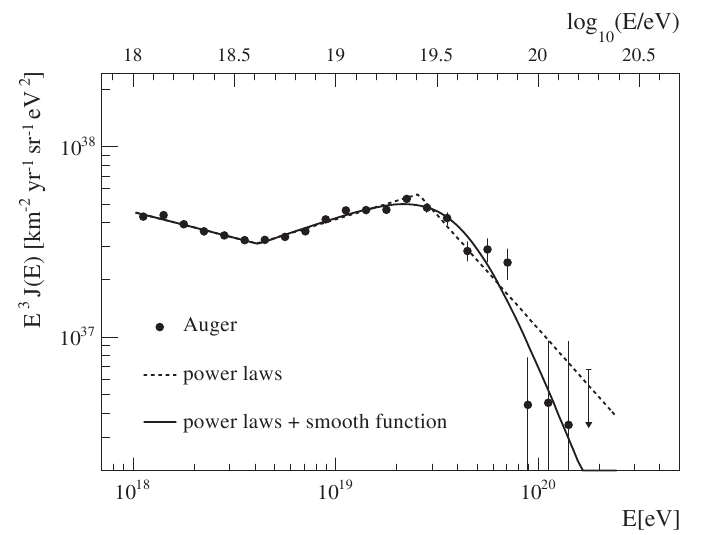
\includegraphics[width=0.75\textwidth]{fig/introduccion/spectrum_withGZK}
		\caption{\label{fig:specGZK} }
		\end{center}
	\end{figure}
	
	\section{Importancia de la detecci\'on de neutrinos c\'osmicos}

\begin{figure}[ht]
	\begin{center}
	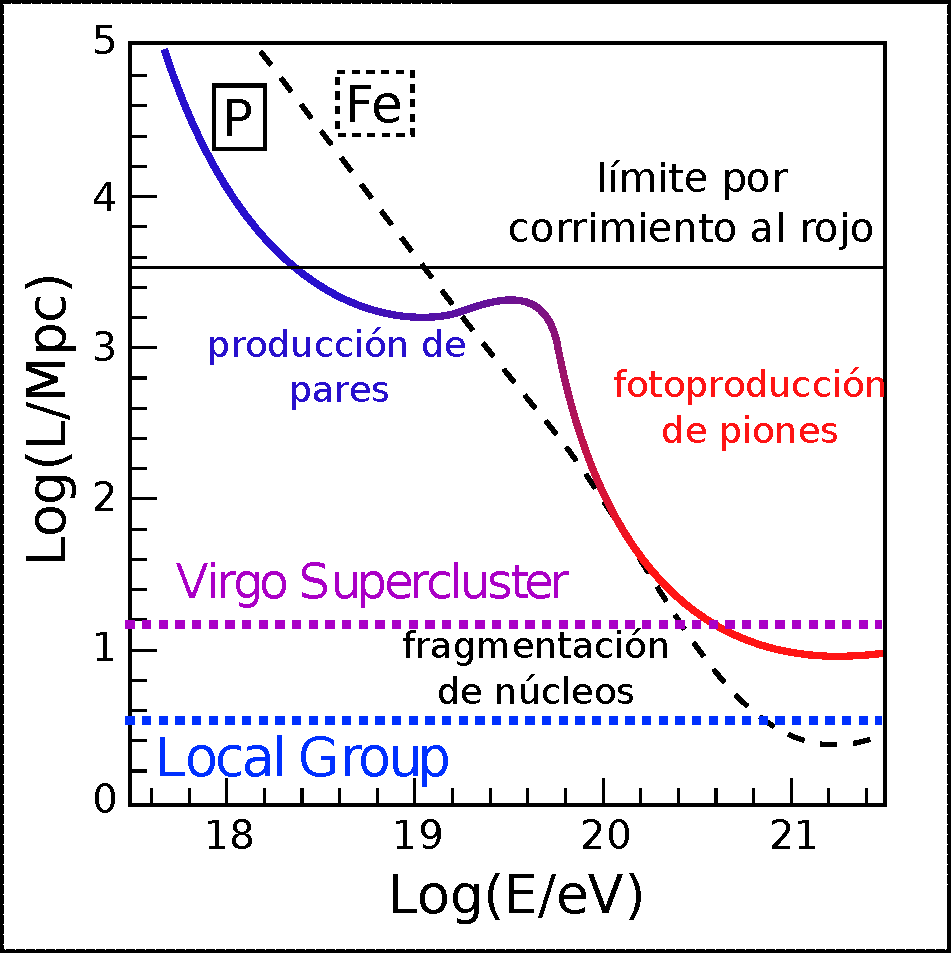
\includegraphics[width=0.75\textwidth]{fig/introduccion/proton_propaga_espanol}
	\caption{\label{fig:protProp} }
	\end{center}
\end{figure}


\begin{figure}[ht]
	\begin{center}
	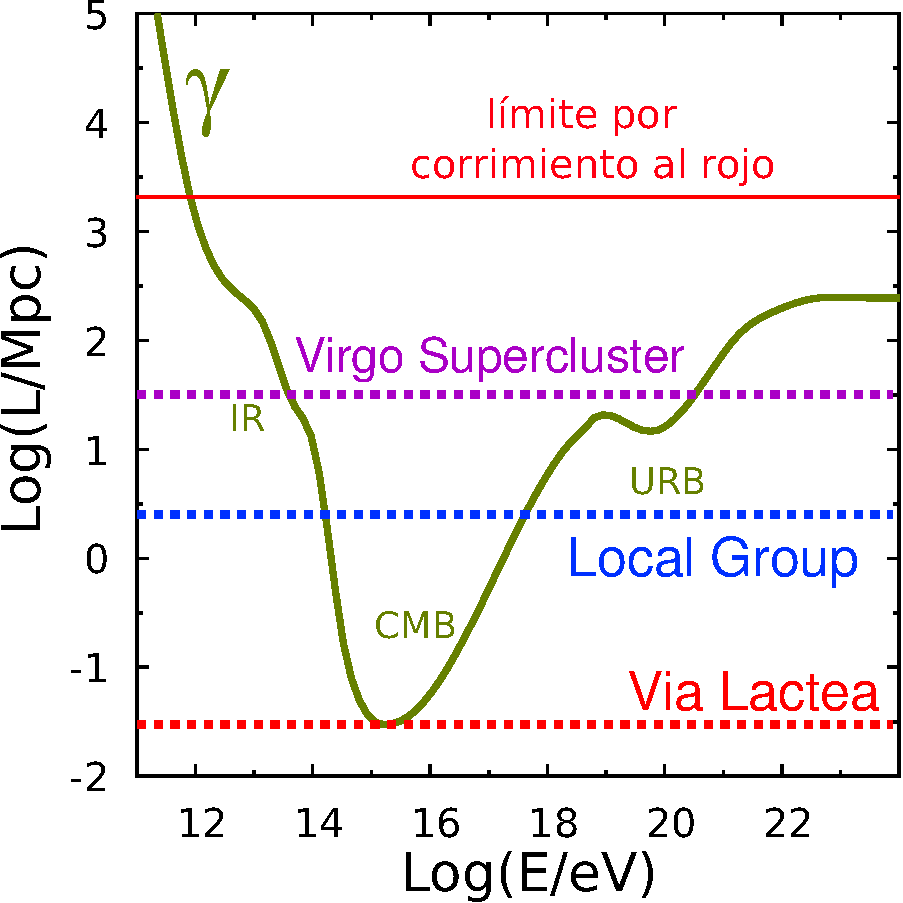
\includegraphics[width=0.75\textwidth]{fig/introduccion/photon_propaga_espanol}
	\caption{\label{fig:photProp} }
	\end{center}
\end{figure}

\section{Posibles fuentes y flujos esperados}

	\subsection{Neutrinos GZK}

	\begin{figure}[ht]
		\begin{center}
		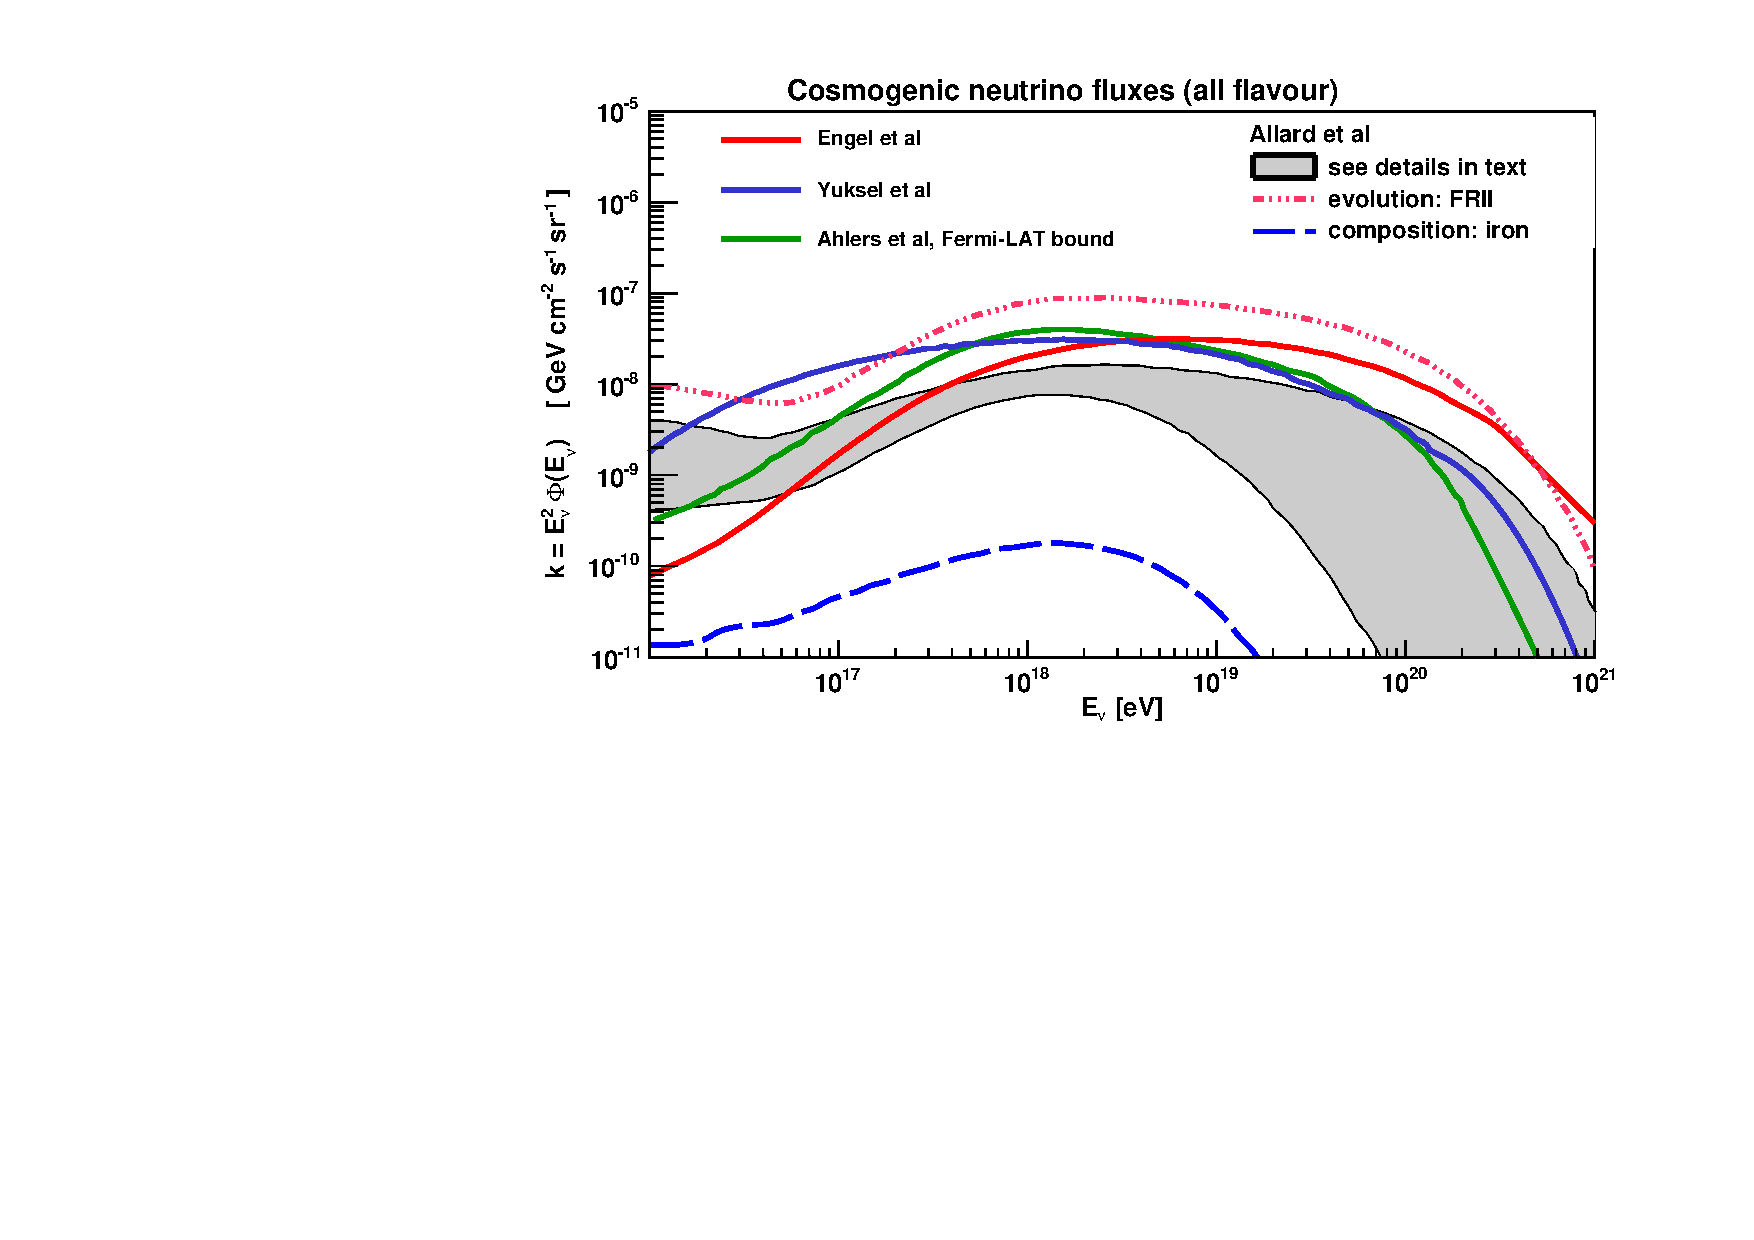
\includegraphics[width=\textwidth]{fig/introduccion/gzk_fluxes}
		\caption{\label{fig:flujosGZK} }
		\end{center}
	\end{figure}
	
	\subsection{AGNs y GRBs}
	
	\begin{figure}[ht]
		\begin{center}
		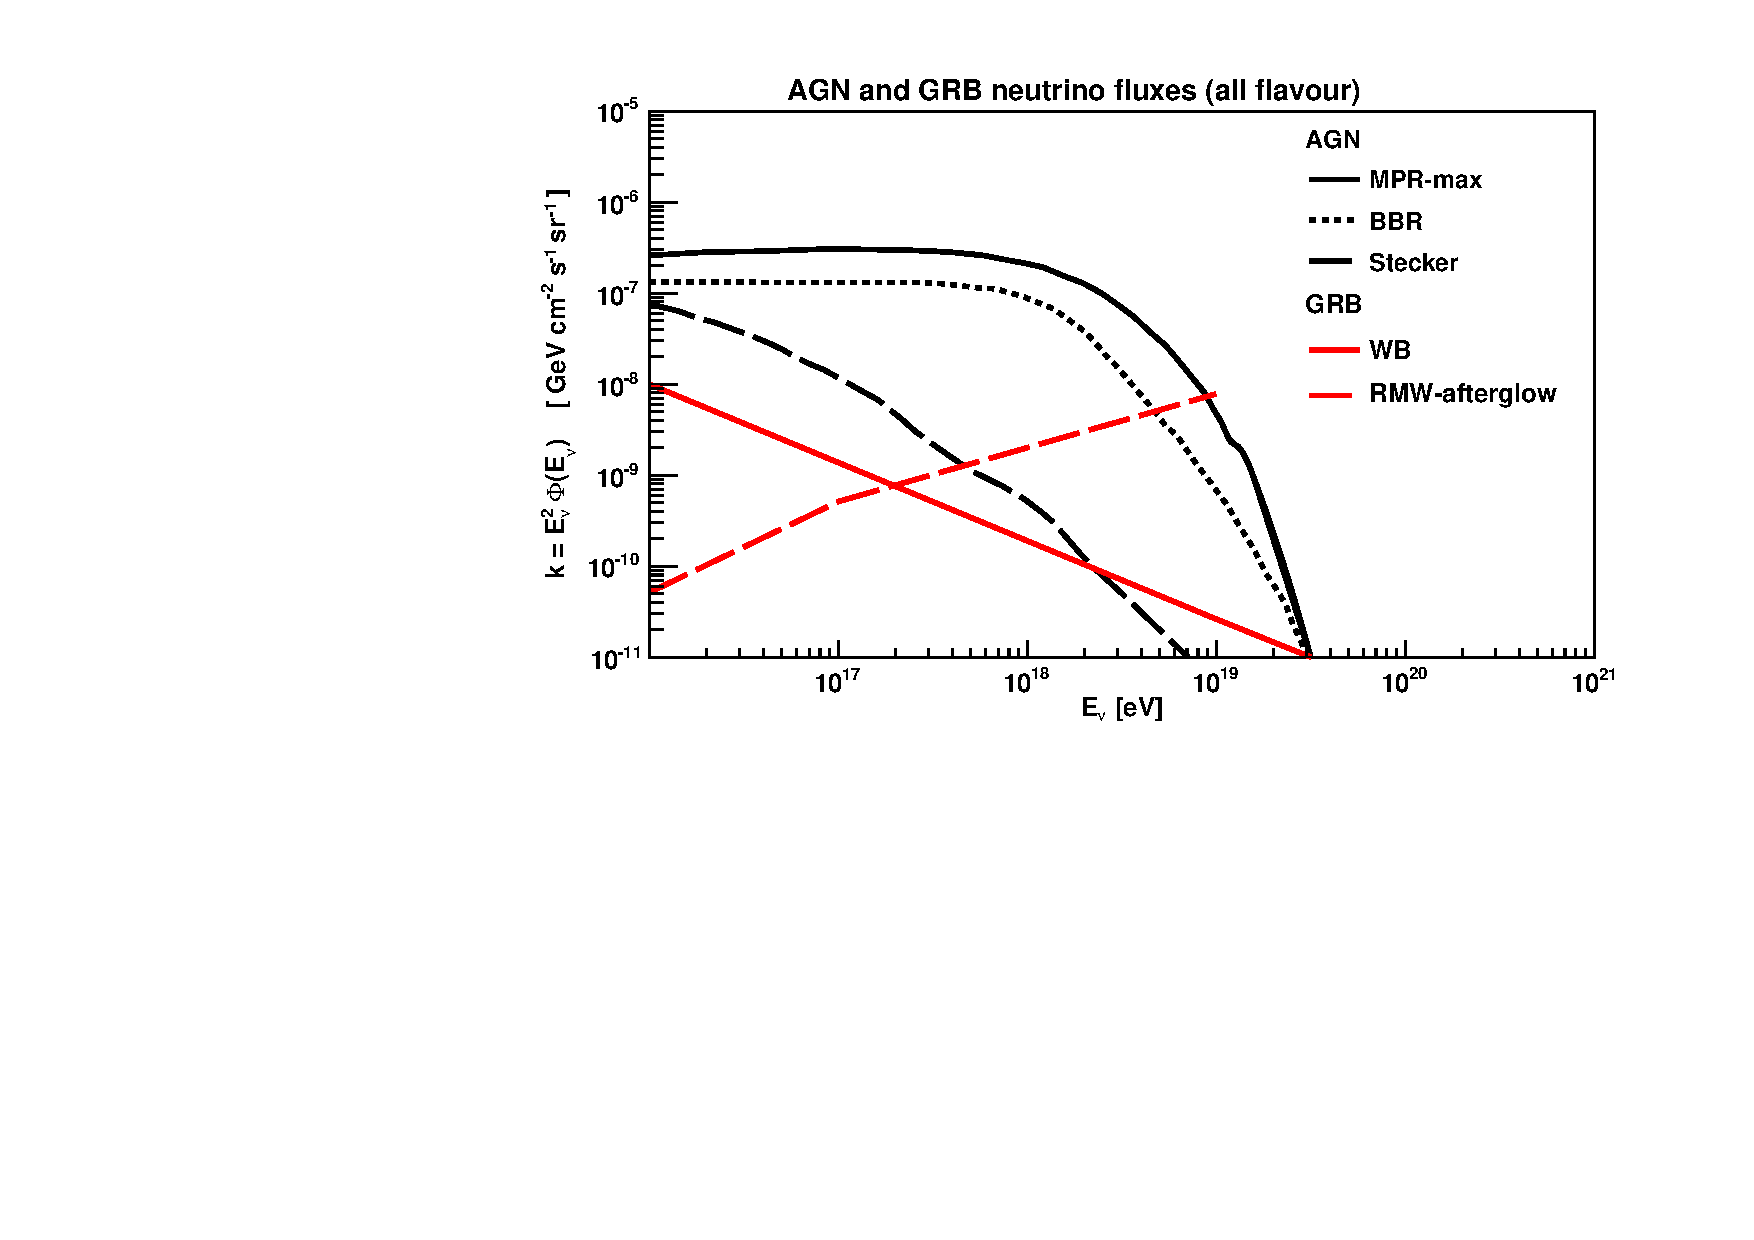
\includegraphics[width=0.75\textwidth]{fig/introduccion/AGN_GRB_nufluxes}
		\caption{\label{fig:flujosAGN} }
		\end{center}
	\end{figure}
	
	\subsection{Fuentes no convencionales}
	
	\begin{figure}[ht]
		\begin{center}
		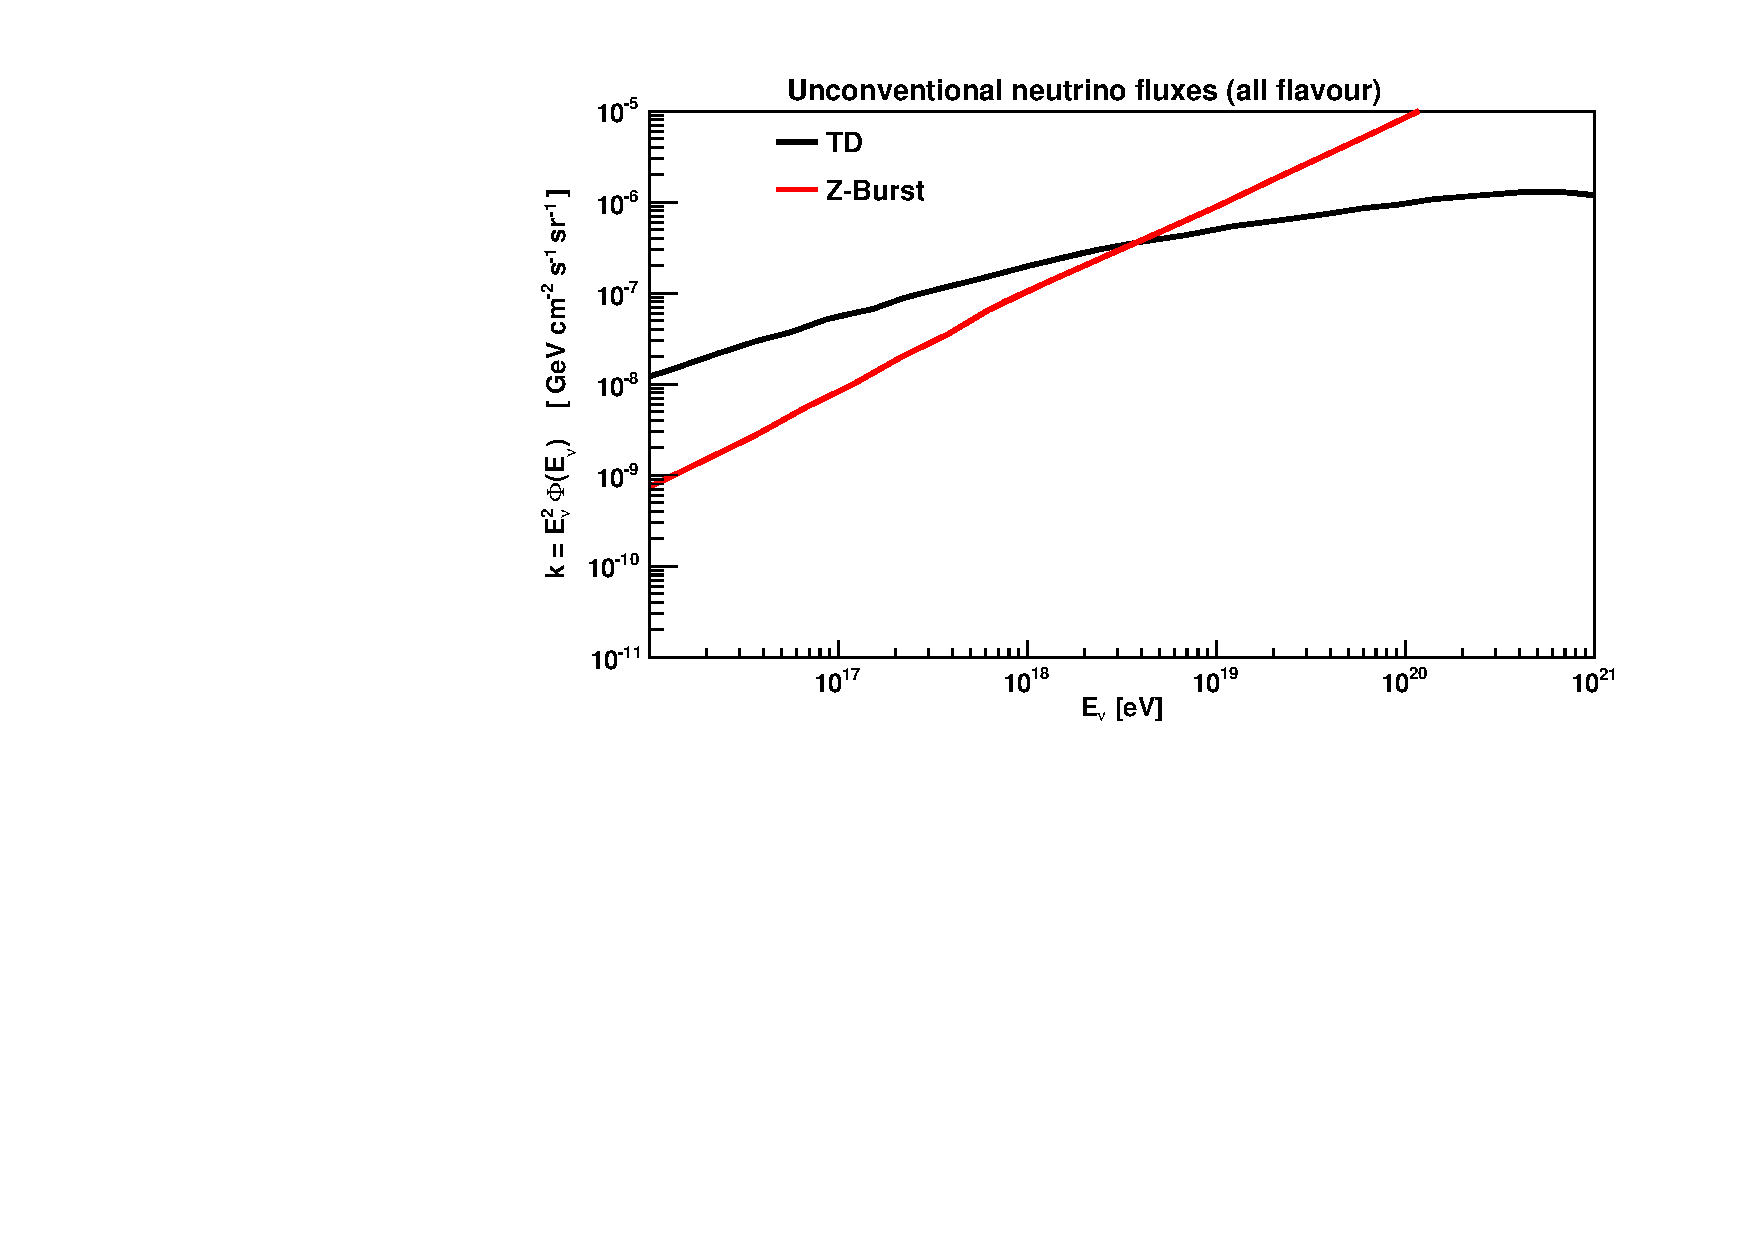
\includegraphics[width=0.75\textwidth]{fig/introduccion/unconventional_nuFluxes}
		\caption{\label{fig:flujosNoConv} }
		\end{center}
	\end{figure}

\section{Búsquedas ne neutrinos cósmicos ultra energéticos}

\section{Nacimiento de la astronom\'ia de neutrinos c\'osmicos}



\mainmatter
% %%%%%%%%%%%%%%%%%%%%%%%%%%%%
% %   Deteccion con Auger
% %%%%%%%%%%%%%%%%%%%%%%%%%%%%
\chapter{Neutrinos c\'osmicos de ultra alta energ\'ia}
\label{ch:NeutrinosUHE}

%
%
%%
%%%
% 	VER EL PROPOSAL DE GRAND!
%%%
%%
%
%
\section{Importancia de los neutrinos cósmicos}


El estudio de rayos c\'osmicos ultra energ\'eticos (UHECR, por su sigla en ingl\'es) ha estimulado en gran medida la actividad experimental y te\'orica en el campo de la astrof\'isica.
Aunque su espectro de energ\'ia ha sido caracterizado en un rango sorprendente, que comprende 14 \'ordenes de magnitud, quedan todav\'ia muchos misterios por resolver, como su origen y sus mecanismos de aceleraci\'on.
En esta direcci\'on, la medici\'on de UHECRs cargados presenta dos grandes limitaciones, su deflexi\'on en los campos magn\'eticos existentes en el cosmos y lo que se conoce como el corte GZK.
A energ\'ias por debajo de los \cant{10^{19.5}}{eV} las trayectorias desde la fuente se ven modificadas debido a la interacci\'on con los campos magn\'eticos gal\'acticos e intergal\'acticos lo que implica que la direcci\'on de arribo de los rayos a la Tierra no apunta a la fuente.
Por otro lado, el corte GZK refiere al mecanismo propuesto por Greisen, Zatsepin y Kusmin~\cite{cite:Greisen,cite:Zatsepin}, que provoca una caída abrupta en el flujo de UHECRs por encima de \cant{5\times10^{19}}{eV}.
Este efecto se debe a la p\'erdida de energ\'ia inducida por la interacci\'on con el fondo c\'osmico de microondas (CMB) via la reacci\'on
%
\begin{equation}
p + \gamma_{\rm CMB}\, \rightarrow\, \Delta^{+}(1232)  \rightarrow p +\pi^{0}\quad {\rm o}\quad n +\pi^{+}
\end{equation}
%
para el caso de protones, o fotodesintegración para núcleos.
La longitud de atenuaci\'on para este proceso es $L_{att}=\frac{L_{int}}{y}$, donde $y$ es la fracci\'on de energ\'ia perdida por longitud de interacci\'on y $L_{int}$ es la longitud de interacci\'on, dada por $L_{int}=(\sigma_{p\gamma}\times n_{\gamma})^{-1}$.
Valores t\'ipicos son $\sigma_{p\gamma}\sim 10^{-28}$~cm$^{2}$, $ n_{\gamma}=410\,{\rm cm}^{-3}$ y $y\sim0.5$\footnote{$y\sim0.2$ a la energ\'ia de corte y se incrementa hasta 0.5.}, resultando en 
% \begin{equation}
$L_{att}=(\sigma_{p\gamma}\times n_{\gamma}\times y)^{-1}\sim 15\mbox{ }{\rm Mpc}$. 
Ya que a estas energ\'ias los rayos c\'osmicos son mayormente extra gal\'acticos, el corte GZK limita la m\'axima energ\'ia que puede ser observada en la Tierra, provocando una supresi\'on del flujo por encima de \cant{50}{EeV}.
En la figura \ref{fig:protProp} se muestra la longitud $L_{att}$ como funci\'on de la energ\'ia para protones y n\'ucleos de hierro. 
Es posible observar como a partir de los \cant{50}{EeV} esta cantidad decae hasta un tama\~no inferior al del Super cluster de Virgo, al alcanzar los \cant{1000}{EeV}.
%
\begin{figure}[ht]
	\begin{center}
	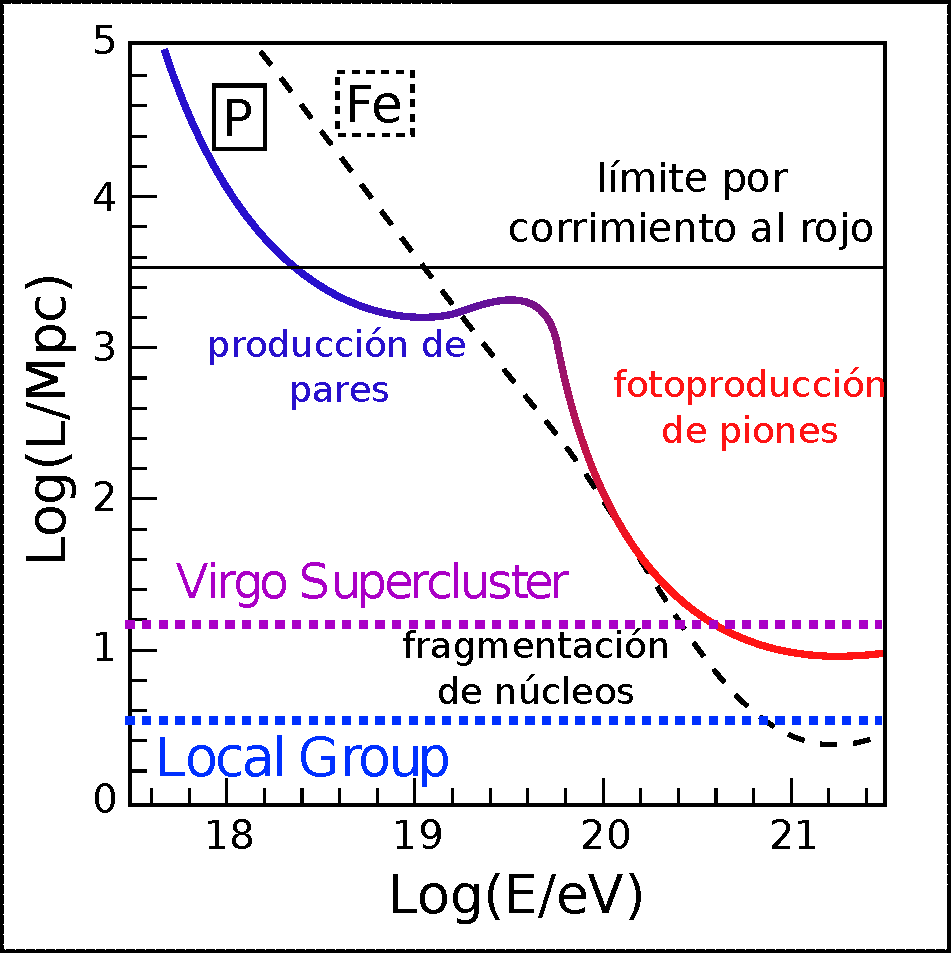
\includegraphics[width=0.55\textwidth]{fig/introduccion/proton_propaga_espanol}
	\caption{\label{fig:protProp} Longitud de atenuaci\'on como funci\'on de la energ\'ia para protones y n\'ucleos de hierro. Se observa que a partir de \cant{50}{EeV} ($\log{E/eV}=18$) esta cantidad decae hasta el tama\~no del Super cluster de Virgo a los \cant{1000}{EeV}.}
	\end{center}
\end{figure}
%

Por otro lado, el observatorio Pierre Auger ha medido el flujo de rayos c\'osmicos combinando un detector de superficie con t\'ecnicas de fluorescencia y ha acumulado suficiente estad\'istica para medir el flujo con precisi\'on hasta \cant{\sim2\times10^{20}}{eV}. 
Tambi\'en pudo corroborar que la supresi\'on del flujo sucede a energ\'ias superiores a los \cant{10^{19.6}}{eV}~\cite{cite:AugerSpectrum}, tal como se observa en la figura \ref{fig:specGZK}.
%
\begin{figure}[ht]
	\begin{center}
	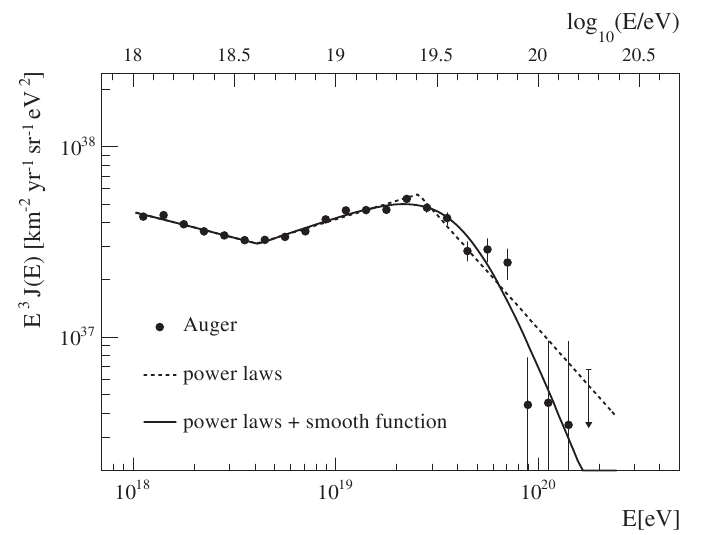
\includegraphics[width=\textwidth]{fig/introduccion/spectrum_withGZK}
	\caption{\label{fig:specGZK} Espectro de UHECRs medido con el observatorio Pierre Auger. En l\'inea punteada se muestra el ajuste por leyes de potencia partidas y en l\'inea llena la dos leyes de potencia y una funci\'on suave. Las barras corresponden al error estad\'istico de cada punto, mientras que el error sistem\'atico representa el $22\%$ de la energ\'ia.}
	\end{center}
\end{figure}

De manera similar, el flujo de fotones ultra energ\'eticos, por encima de \cant{\sim10^{14}}{eV}, no puede ser de naturaleza extra gal\'actica, debido a la producci\'on de pares en la interacci\'on con fotones del fondo de microondas, seg\'un\cite{cite:photonInt1,cite:photonInt2}:
%
\begin{equation}
\gamma_{UHE} + \gamma_{CMB} \rightarrow e^- + e^+
\end{equation}
%
En la figura \ref{fig:photProp} se grafica la longitud de atenuaci\'on\footnote{Corresponde a la distancia necesaria para que el flujo decaiga a la mitad.} de los fotones como funci\'on de la energ\'ia.
%
\begin{figure}[ht]
	\begin{center}
	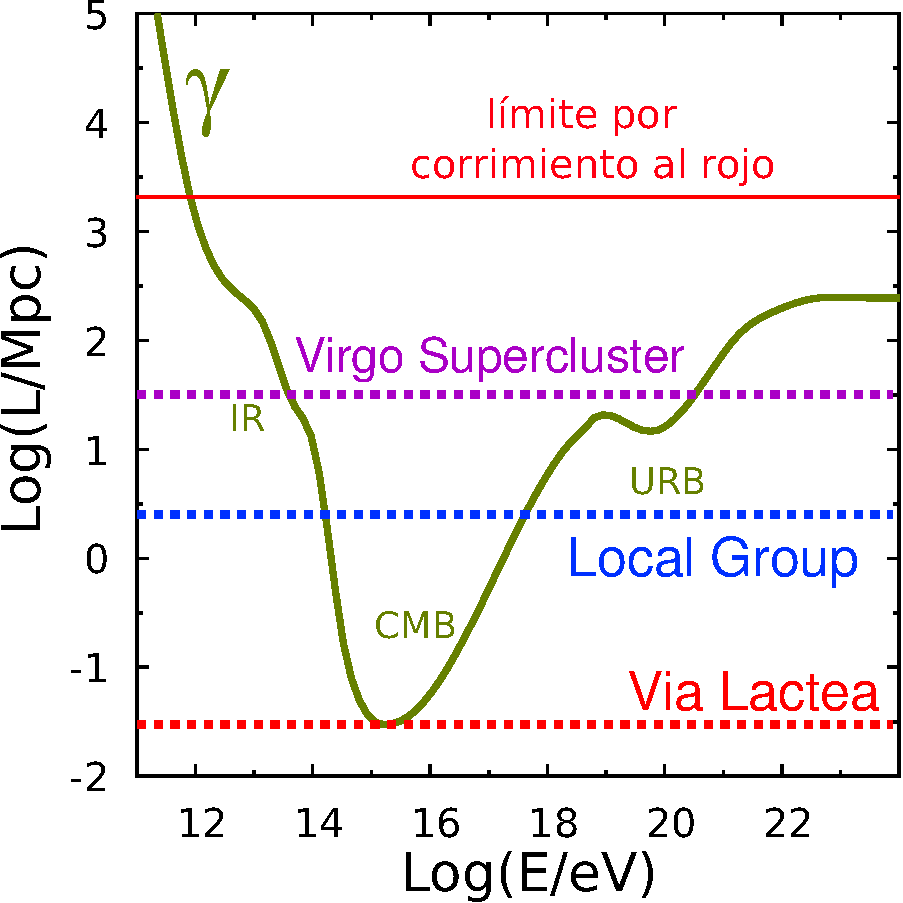
\includegraphics[width=0.55\textwidth]{fig/introduccion/photon_propaga_espanol}
	\caption{\label{fig:photProp} Longitud de atenuaci\'on para fotones. Los $\gamma$ con energ\'ias entre \cant{10^{14}}{eV} y \cant{10^{18}}{eV} pr\'acticamente no pueden alcanzar la Tierra desde distancias mayores a \cant{1}{Mpc}. Las etiquetas IR, CMB y URB (ver texto) corresponden al fondo dominante contra el que interact\'uan los $\gamma_{UHE}$.}
	\end{center}
\end{figure}
%
Dependiendo de la energ\'ia, los $\gamma_{UHE}$ pueden interactuar tambi\'en con el fondo de radiaci\'on infrarroja (IR)\cite{cite:IR} y con el fondo de radio universal (URB)\cite{cite:URB}.

Como consecuencia el tercer mensajero $-$ el neutrino $-$ cobra una importancia adicional, lo que convirti\'o su detecci\'on en uno de los mayores logros de la astrof\'isica contempor\'anea.
Esto se debe a que los neutrinos no sufren ninguna de las desventajas mencionadas hasta el momento. 
Debido a que interact\'uan mediante interacci\'on d\'ebil y a que su secci\'on eficaz resulta extremadamente peque\~na, pueden viajar distancias cosmol\'ogicas e incluso escapar de la regi\'on en la que fueron producidos casi sin p\'erdidas de energ\'ia.
Por otro lado, debido a que son el\'ectricamente neutros su trayectoria no se ver\'a deflectada debido a la interacci\'on con los campos magn\'eticos intra y extra gal\'acticos.
Por este motivo, la direcci\'on de arribo de los neutrinos c\'osmicos detectados guardar\'a completamente la informaci\'on del lugar del universo en el que fueron producidos.
Por estos motivos, representan una opci\'on \'unica que permite detectar directamente posibles fuentes de UHECRs.

En este cap\'itulo se presenta una discusi\'on sobre las posibles fuentes y flujos de neutrinos c\'osmicos ultra energ\'eticos 
%a saber, el mecanismo GZK, n\'ucleos de galaxias activos (AGN) y explosiones de rayos gamma (GRB).
%Tambi\'en se realizar\'a un recuento 
y sobre los esfuerzos experimentales en este campo.

\section{Posibles fuentes y flujos esperados}

Existen varios modelos en la literatura que predicen flujos de neutrinos c\'osmicos ultra energ\'eticos.
La supresi\'on observada en el flujo por encima de los \cant{50}{EeV} refuerza la idea de la existencia de un flujo difuso de neutrinos cosmog\'enicos.
En este caso, estos son producidos durante la propagaci\'on de un UHECR a trav\'es del universo. 
Adem\'as pueden ser producidos en la aceleraci\'on de protones y n\'ucleos en n\'ucleos de galaxias activos (AGN)\cite{cite:nuAGN} o por producci\'on de fotopiones en explosiones de rayos gamma (GRB)\cite{cite:nuGRB}.
% Detectores como AMANDA o IceCube, su sucesor, se encuentran bien posicionados para realizar b\'usquedas de fuentes con espectros de ley de potencia fuertes ($\propto E^{-2}$) en el rango que comprende desde el TeV  hasta el PeV. 
% Para fuentes cuyo flujo presenta un m\'aximo en energ\'ias por encima de los \cant{100}{PeV} el flujo predicho resulta ser peque\~no, requiriendo detectores con mayor exposici\'on.

% Otros posibles mecanismos de producci\'on de neutrinos c\'osmicos estan relacionados con el decaimiento de part\'iculas ex\'oticas extremadamente masivas tales como defectos topol\'ogicos\cite{cite:nuTopDefects}, o con la interacci\'on de neutrinos energ\'eticos con el fondo de neutrinos del Big-Bang via la resonancia Z-burst\cite{cite:nuZBurst_init}.
% Estos flujos, que pretend\'ian explicar el origen de los rayos c\'osmicos ultra energ\'eticos, han sido fuertemente constre\~nidos por los experimentos m\'as recientes\cite{cite:nuConstraintsTD}.
% En las siguientes secciones se desarrollas las ideas enumeradas hasta aqu\'i.

	\subsection{Neutrinos GZK}
	\label{sbsc:introGZK}
	Greisen, Zatsepin and Kusmin propusieron que los rayos c\'osmicos cuya energ\'ia supere los \cant{5\times10^{19}}{eV}, al propagarse por el universo interactuar\'an con el fondo de microondas produciendo neutrinos, seg\'un la ecuaci\'on \ref{eq:pionDecay}.
	\begin{equation}\label{eq:pionDecay}
	\pi^{+} \rightarrow \mu^{+}+ \nu_{\mu} \rightarrow e^{+} + \nu_{e} + \bar{\nu}_{\mu} + \nu_{\mu}
	\end{equation}
	
	La presencia del corte GZK indica que los UHECRs provienen de fuentes extra galácticas.
	Esto implica que los llamados neutrinos GZK son el flujo más verosimil entre todas las posibles teorías. 
	Sin embargo, su cálculo contiene una gran cantidad de supuestos que se traducen en incertezas en el resultado final.
	Los factores m\'as relevantes en su determinaci\'on son los siguientes~\cite{cite:nuEngel,cite:nuAve,cite:nuAhlers1,cite:nuAllard1,cite:nuYuksel}:
	
	\textbf{Composici\'on de los UHECRs}: las primeras predicciones sobre el flujo de neutrinos cosmol\'ogicos asum\'ian que los primarios son protones, mientras que recientemente ha surgido evidencia que éstos podrían ser núcleos, como $^{56}{\rm Fe}$, $^{4}{\rm He}$, $^{16}{\rm O}$, o mezclas entre ellos y protones\cite{cite:nuAve,cite:nuHooper}.
	Los n\'ucleos m\'as pesados pierden energ\'ia por foto-desintegraci\'on, produciendo una cadena de n\'ucleos secundarios y fotopiones, los que al decaer generan neutrinos.
	Adem\'as, se predicen fujos de antineutrinos electr\'onicos via decaimiento de neutrones\cite{cite:nuFeComposition}, pero su energ\'ia resulta baja para ser detectados por Auger.
	Los flujos esperados de una composici\'on primaria no pura son más peque\~nos que bajo la hipótesis de una composici\'on exlusiva de protones\cite{cite:nuHooper}.
	En particular, la energ\'ia por nucle\'on luego de una fotodesintegraci\'on resulta mucho menor que la del primario, lo que desfavorece la generaci\'on de neutrinos GZK.
	Existen tambien modelos en los que se propone una distribuci\'on de primarios en acuerdo con la composici\'on observada en los rayos c\'osmicos gal\'acticos\cite{cite:nuAllard1}.
	Como consecuencia de estas suposiciones los flujos predichos pueden fluctuar en un \'orden de magnitud.
	 
	En particular, resultados recientes de Auger indican, aunque con cierto nivel de debate, que el flujo de UHECRs se encuentra dominado por n\'ucleos pesados\cite{cite:augerComposition}, mientras que mediciones de HiRes y Telescope Array\cite{cite:taComposition} han concluído lo opuesto.
	Si se llegase a dar una observaci\'on por encima de las predicciones para primarios pesados, se podr\'ia echar luz sobre esta situación.
	 
	\textbf{Perfil de energ\'ia}: el espectro energ\'etico de los rayos c\'osmicos en el punto de inyecci\'on se supone que sigue t\'ipicamente una ley de potencia:
	%
	\begin{equation}
		\frac{dN}{dE}=P_{0} \times E^{-\alpha} \times \exp{(-\frac{E}{E_{c}})}
	\end{equation}
	%
	donde $P_0$ es una normalizaci\'on y el \'indice espectral $\alpha$ toma valores entre 1.8 y 2.7, siendo $\alpha\sim2.3$ el m\'as favorecido.
	El corte de energ\'ia en la inyecci\'on, $E_c$, se considera que vale entre \cant{10^{20}}{eV} y \cant{10^{23}}{eV}.
	Tanto $\alpha$ como $E_c$ dependen de las caracter\'isticas de la fuente y del mecanismo de aceleraci\'on de los rayos c\'osmicos.
	Una vez que estos valores son elegidos, la normalizaci\'on $P_0$ se utiliza para hacer coincidir el flujo con el observado experimentalmente en la Tierra.
	Valores grandes de $\alpha$ o peque\~nos de $E_c$ producen flujos de neutrinos m\'as peque\~nos a energ\'ias de observaci\'on de Auger debido a la disminuci\'on en la cantidad de protones de altas energ\'ias en la fuente.
	
	\textbf{Modelo cosmol\'ogico}: la cosmolog\'ia del universo es otro factor que genera incerteza en la magnitud del flujo de neutrinos GZK. 
	En la actualidad, observaciones astrof\'isicas apuntan hacia modelos con una constante cosmol\'ogica $\Lambda$\cite{cite:Lambda}, en contraste con los c\'alculos de mediados de la d\'ecada del 90, que supon\'ian un universo de Einstein-de Sitter ($\Omega_{M}=1$). 
	El modelo favorecido actualmente posee $\Omega_{\Lambda}=0.7$ y $\Omega_{M}=0.3$\cite{cite:LambdaM}, lo que significa que la energ\'ia oscura representa alrededor del 70\% de la energ\'ia del universo.
	Como consecuencia, el universo debi\'o haberse estado expandiendo más lentamente en el momento en el que los flujos cosmol\'ogicos se generaron, ocasionando un incremento en los flujos esperados para corrimientos al rojo grandes.
	Engel et al. \cite{cite:nuEngel} compararon el flujo derivado de los dos modelos cosmol\'ogicos y encontraron que valores de $\Omega_{\Lambda}=0.7$ podr\'ian ocasionar hasta un 60\% de incremento en el flujo de neutrinos esperado.
	
	\textbf{Evoluci\'on cosmol\'ogica}: la predicci\'on de los flujos de neutrinos dependen fuertemente de la evoluci\'on cosmol\'ogica de las fuentes de rayos c\'osmicos.
	Existen al menos 4 modelos de evoluci\'on utilizados comunmente en la bibliograf\'ia:
	\begin{enumerate}
	 \item Sin evoluci\'on;
	 \item Star Formation Rate;
	 \item Active Galactic Nuclei-FRII (FRII) y
	 \item Strong Gamma Ray Burst (GRB).
	\end{enumerate}
	
	Las diferencias inducidas por esta elecci\'on pueden modificar el flujo esperado en un \'orden de magnitud.
	
	\textbf{Secci\'on eficaz protón-fot\'on}: el ritmo de producci\'on de neutrinos mediante la interacci\'on:
	%
	\begin{displaymath}
	p + \gamma_{\rm CMB}\, \rightarrow\, \Delta^{+}  \rightarrow p +\pi^{0}\quad {\rm or}\quad n +\pi^{+}
	\end{displaymath}
	%
	viene dado por la secci\'on eficaz prot\'on-fot\'on, $\sigma_{p\gamma}$.
	Las mediciones de esta cantidad provienen de aceleradores, por lo que se encuentran bien caracterizadas en un rango de energ\'ias totalmente distinto al que corresponde a la producci\'on de neutrinos.
	
	\textbf{Oscilaciones de neutrinos}: en el decaimiento de un pi\'on, la relaci\'on con la que se producen neutrinos mu\'onicos y electr\'onicos es $2:1$. 
% 	En este trabajo, al menos que se especifique lo contrario, hablar de neutrinos de cierto sabor $\nu_x$, har\'a referencia al par $\nu_x + \bar\nu_x$.
	Dado que los neutrinos oscilan, al recorrer distancias cosmol\'ogicas la relaci\'on entre los flujos $\nu_e :\nu_\mu :\nu_\tau$ de $1:2:0$ en la fuente se transformar\'a en una relaci\'on $1:1:1$ en la Tierra.

	%
	Aunque la existencia de los neutrinos cosmog\'enicos tiene una base teórica sólida, los flujos predichos para este mecanismo var\'ian cuatro \'ordenes de magnitud.
	Algunas de estas predicciones se muestran en la figura \ref{fig:flujosGZK} para los tres sabores de neutrinos.
	
	\begin{figure}[ht]
		\begin{center}
		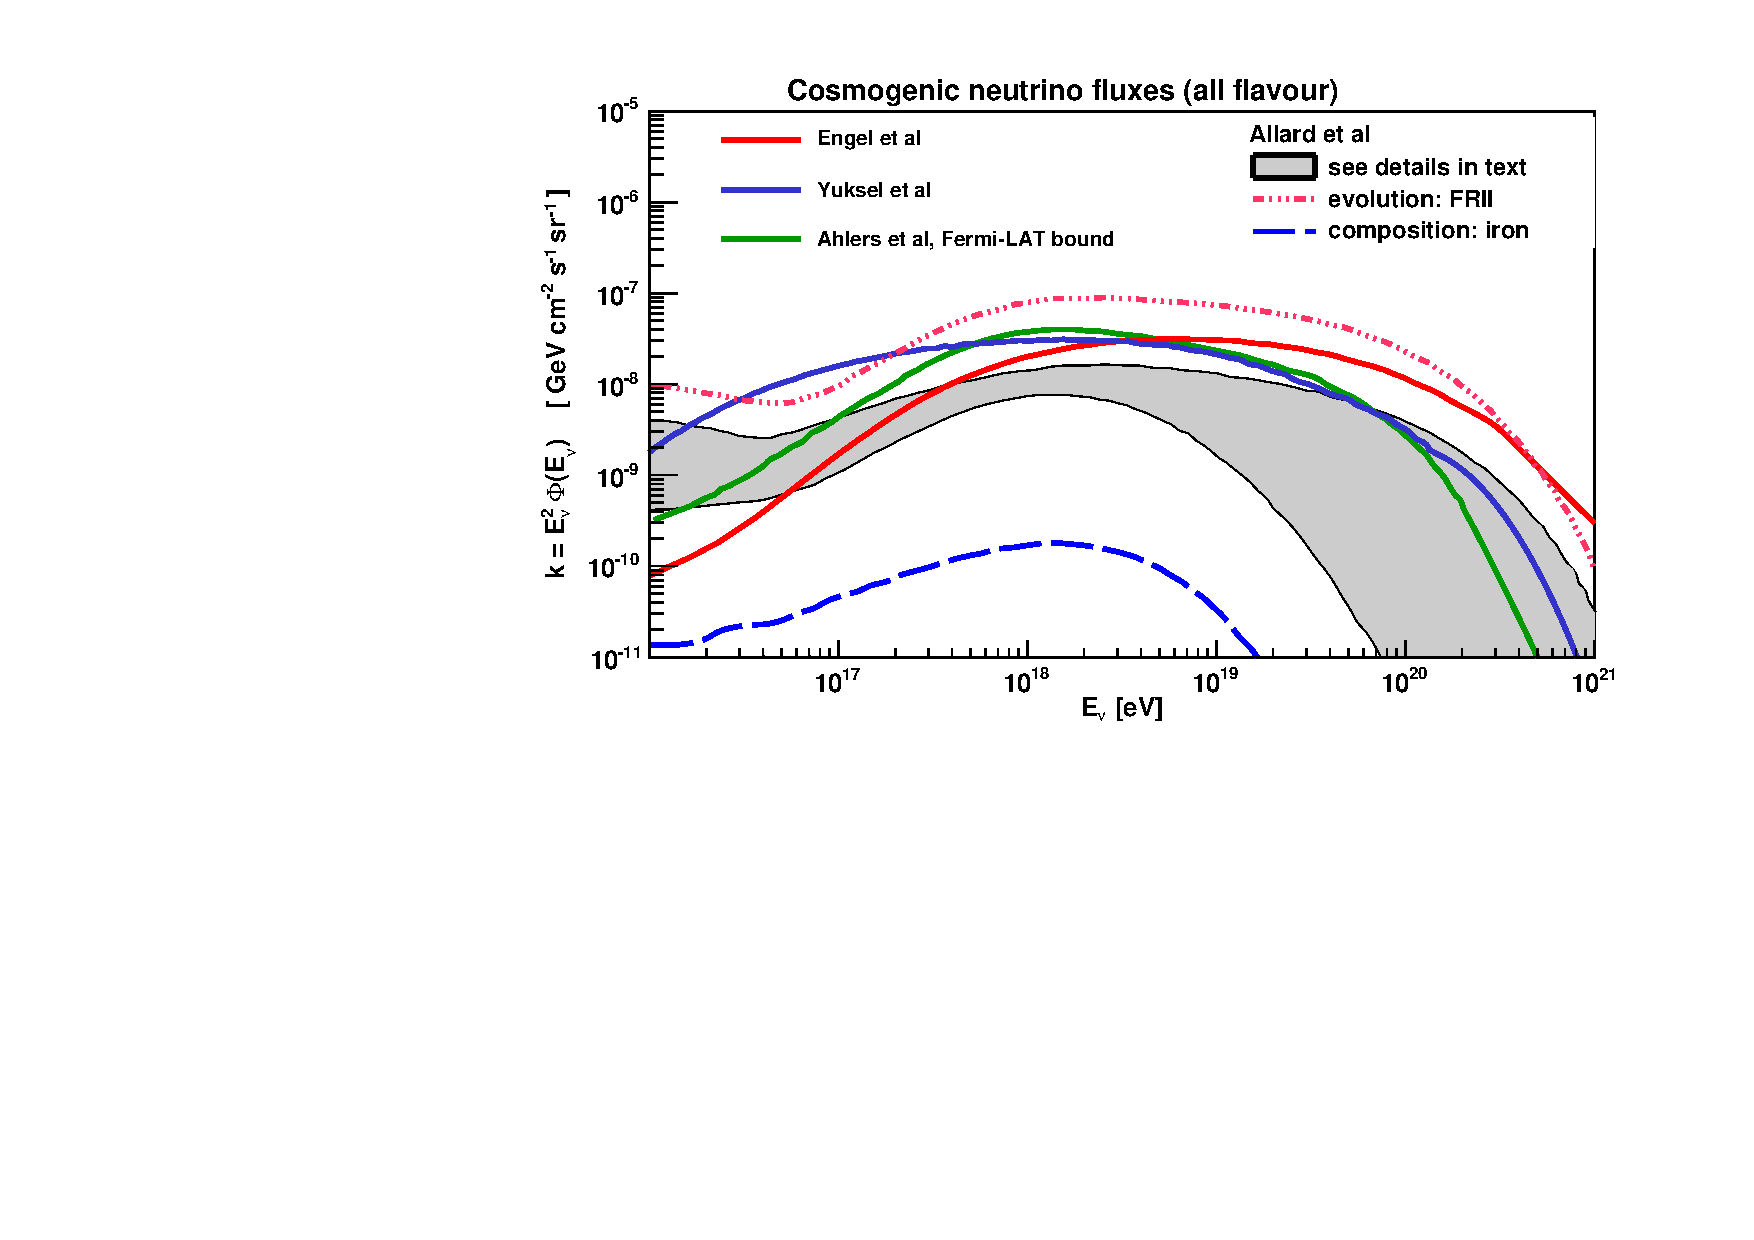
\includegraphics[width=\textwidth]{fig/introduccion/gzk_fluxes}
		\caption{\label{fig:flujosGZK} Flujos cosmog\'enicos para los tres sabores de neutrinos. En todos los casos el modelo cosmol\'ogico usado corresponde a $\Omega_{\Lambda}=0.7$ y $\Omega_{M}=0.3$. 
		En rojo se muestra un flujo GZK t\'ipico para una composici\'on pura de protones, un \'indice $\alpha$ = 2 y \cant{E_{c}=10^{21.5}}{eV}\cite{cite:nuEngel}.
% 		En linea azul s\'olida
% In solid light blue the GRB model for the cosmological evoultion is used\cite{cite:nuYuksel}.
% % In solid green Ref.\cite{cite:nuAhlers1} where they make a prediction using also the measurements of the Fermi-LAT experiment.
% In solid green a prediction using the measurements of the Fermi-LAT experiment\cite{cite:nuAhlers1}.
% The shaded area is obtained from Ref.\cite{cite:nuAllard1}, bracketing a wide range a parameters: 
% several source evolution models (not including uniform and FRII), 
% for pure protons and a mixed Galactic composition. 
% Including the uniform source evolution would lower the prediction by almost an order of magnitude.
% The pink dot-dashed line corresponds to an optimistic scenario with a FRII strong source evolution case with a pure proton composition, 
% % dip transition model 
% and $E_{c}=10^{21.5}$~eV\cite{cite:nuAllard1}. 
% The blue dashed lineis an extreme pessimistic scenario with pure
% iron composition and uniform evolution\cite{cite:nuAllard1}.
% % $E_{c}$ = 1021.5 eV. For the cosmological evolution of the cosmic ray sources, ${\cal H}$(z), they use the
% % aforementioned QSO model with the parameterization of Ref. [33], as given in Eqn.1.7. The
% % default cosmological assumption used is the model with
% 		
		}
		\end{center}
	\end{figure}
	
	\subsection{AGNs y GRBs}
	Los n\'ucleos de galaxias activos (AGN) pueblan de manera isotr\'opica el cielo y representan algunos de los objetos m\'as luminosos en el espacio, con emisiones en el \'orden de los \cant{10^{45\pm3}}{erg/s}\cite{cite:GHZ}.
	Por este motivo no s\'olo son considerados unos de los m\'as fiables candidatos a fuentes de UHECRs, sino que varios autores predicen flujos medibles de neutrinos si la regi\'on de aceleraci\'on se encuentra rodeada de suficiente cantidad de materia.
	
	Se cree que la enorme radiaci\'on emitida por los AGNs se alimenta de la energ\'ia gravitacional liberada por la materia que cae hacia su centro, en el que se ubica un agujero negro super masivo.
	Durante este proceso, el momento angular provoca que parte del material forme un disco de acreci\'on mientras que otra parte se vea despedida hacia chorros perpendiculares al mismo.
	En tal proceso, los shocks turbulentos aceleran part\'iculas hacia altas energ\'ias.
	De esta manera, una parte significativa de la energ\'ia gravitatoria es transferida a part\'iculas ultra relativistas, via el mecanismo de Fermi de primer orden\cite{cite:Fermi1}.
	Por otro lado, la fricci\'on convierte la materia en plasma, que produce un fuerte campo magn\'etico.
	Las colisiones entre los protones ultra relativistas con el intenso campo de fotones del AGN produce neutrinos de alta energ\'ia mediante $p\gamma \rightarrow \pi^{+} + n$ y el subsecuente decaimiento $\pi^{+} \rightarrow \mu^{+} + \nu_{\mu}$ seguido de $\mu^{+} \rightarrow e^{+} + \nu_{e} + \bar{\nu_{\mu}}$.
	
	Otros modelos proponen que los protones colisionan con part\'iculas de gas y polvo, provocando $pp\,\rightarrow\,\pi s + X$.
	Como en el mecanismo GZK, los neutrinos incluidos inicialmente son $\nu_\mu$ y $\nu_e$ pero las oscilaciones homogeneizan los flujos entre sabores al llegar a la Tierra.
	
	Dependiendo del lugar en que la producci\'on de neutrinos se lleve a cabo, existen dos tipos de modelos de producci\'on en AGNs: AGN core y AGN jet.
	En el primer caso, propuesto inicialmente por Stecker et. al.\cite{cite:nuAGN}, los protones acelerados interact\'uan con el campo de fotones dentro del n\'ucleo del AGN. 
	En el segundo modelo, dos jets relativistas emitidos perpendicularmente al disco de acreci\'on formando l\'obulos. 
	Los protones son acelerados mediante el mecanismo de Fermi para luego interactuar con fotones del jet y producir neutrinos.
	Su flujo puede ser estimado midiendo la luminosidad para diferentes corrimientos al rojo, como en \cite{cite:Protheroe1}. Por otra parte, Mannheim et al. \cite{cite:Mannheim1}, calcularon el m\'aximo flujo posible proveniente de AGNs a partir de funciones de evoluci\'on de fuentes para blazares, uno de los tipod de AGNs.
	
	Las explosiones de rayos gamma (GRBs) son flashes de fotones $\gamma$ emitidos por fuentes puntuales.
	Estas, representas unas de las explosiones más fuertes del universo y una posible fuente de neutrinos c\'osmicos ultra energ\'eticos.
	Su emisi\'on ha sido calculada bajo distintas condiciones.
	%
	\begin{enumerate}
	 \item En los modelos de tipo \emph{bola de fuego} o GRB fireball~\cite{cite:grb_Waxman1,cite:grb_Waxman2} la emisi\'on de fotones se produce como producto de colisiones de plasma que se mueve de manera relativista dentro de un chorro de materia (la bola de fuego).
	 Posteriormente el material expulsado colisiona con el medio material externo (por ejemplo el medio interestelar), produciendo radiaci\'on en un ancho de banda amplio, que comprende desde los rayos X y ultra violetas hasta el visible, conocido como el GRB afterglow.
	 Por otro lado, los electrones y protones acelerados en el jet producen la erupci\'on de fotones de alta energ\'ia mediante radiaci\'on de sincrotr\'on y efecto Compton inverso.
	 Estos fotones de alta energ\'ia interact\'uan con los del afterglow y protones o neutrones del jet produciendo neutrinos ultra energ\'eticos via producci\'on de fotopiones.
	 \item Otro modelo de GRB bastante difundido consiste en los llamados ``modelos de supernova''~\cite{cite:grb_Supernova}. 
	 En estos, protones de la cáscara remanente de las supernovas, expulsadas antes del GRB, interact\'uan con los fotones emitidos durante el mismo generando neutrinos ultra energ\'eticos, nuevamente via producci\'on de fotopiones.
	\end{enumerate}
	%
	En la figura \ref{fig:flujosAGN} se muestran los flujos esperados para algunos modelos de AGN y GRB.
	\begin{figure}[ht]
		\begin{center}
		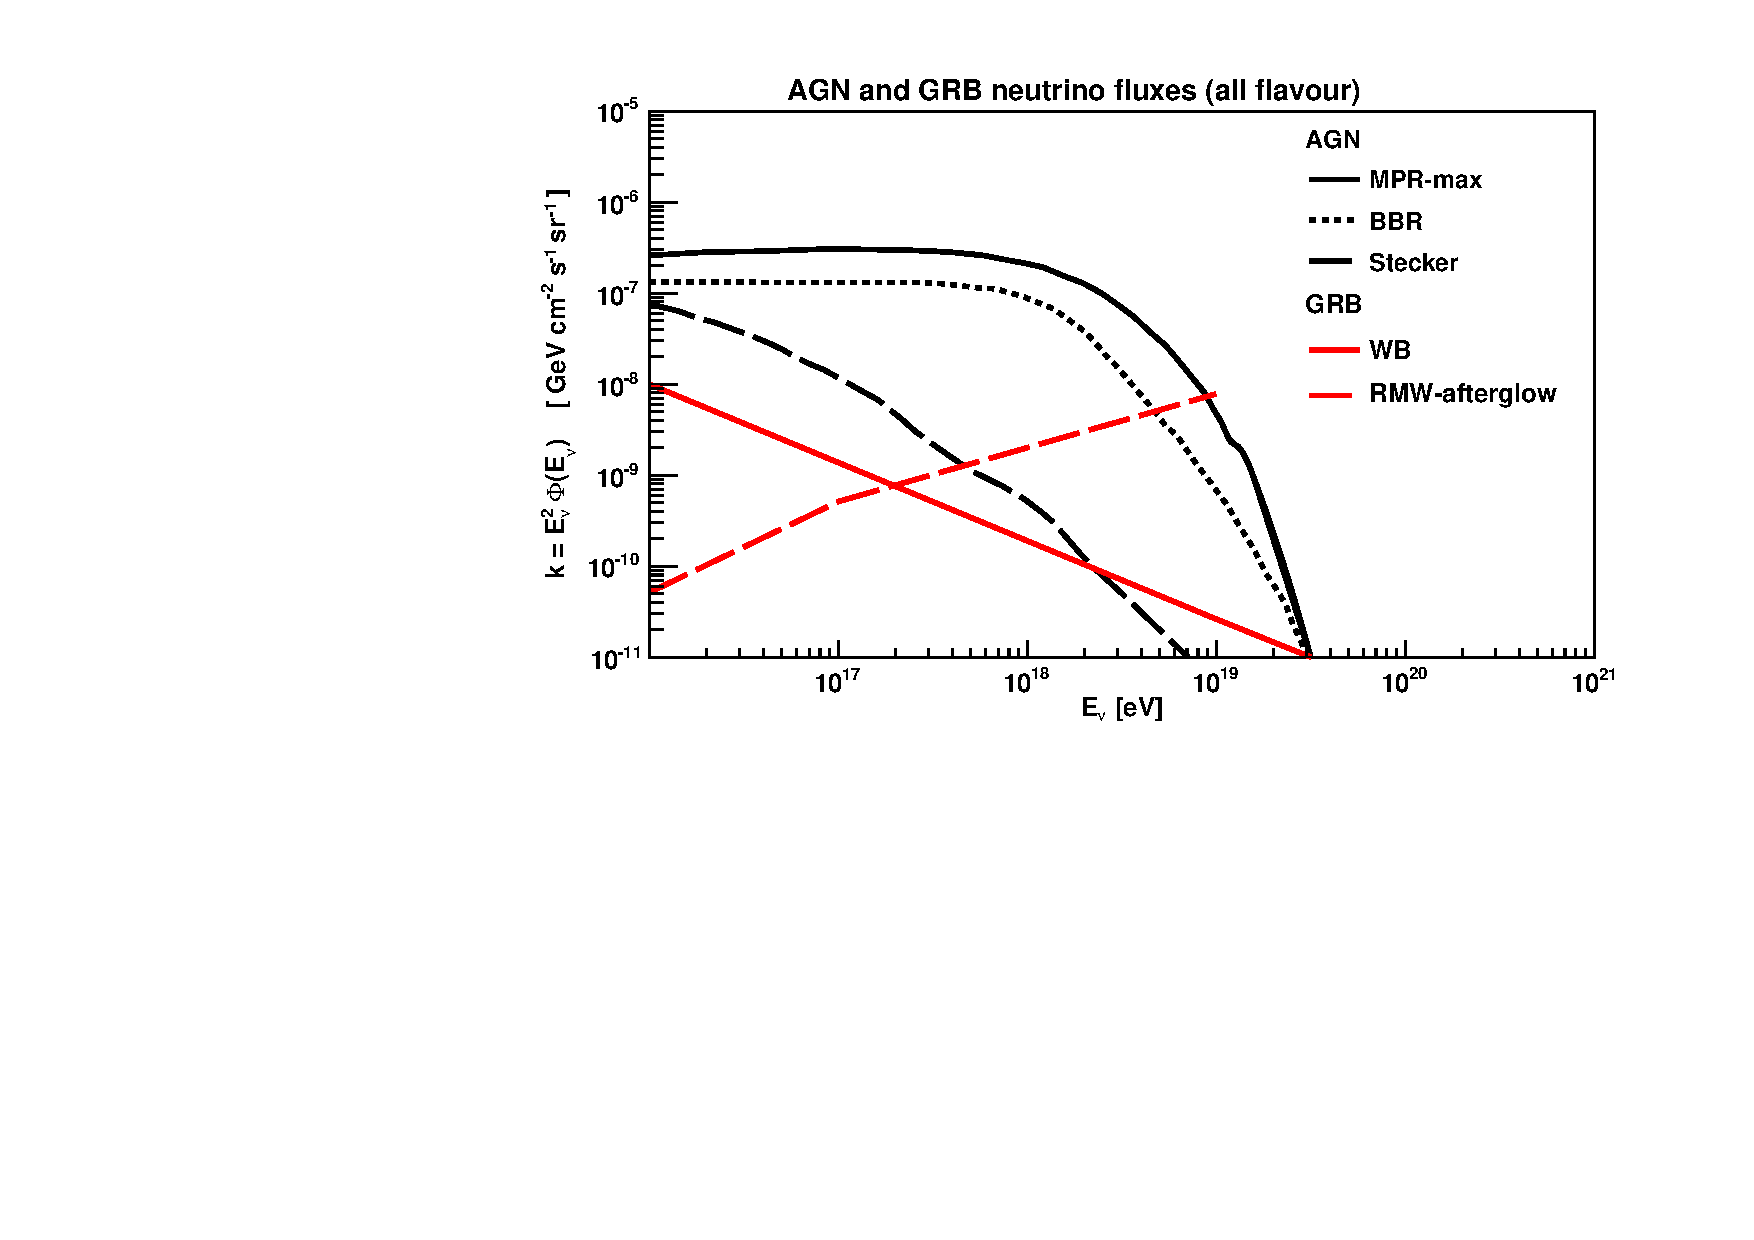
\includegraphics[width=0.75\textwidth]{fig/introduccion/AGN_GRB_nufluxes}
		\caption{\label{fig:flujosAGN} Flujos predichos para AGNs y GRBs. En negro se muestran tres modelos de AGNs\cite{cite:Mannheim1,cite:BBR,cite:SteckerAGN}, mientras que en rojo dos para GRBs\cite{cite:grb_Waxman2,cite:grb_Supernova}.}
		\end{center}
	\end{figure}
	
	\subsection{L\'imite te\'orico al flujo de neutrinos}
	
	E.\ Waxman y J.\ Bahcall~\cite{cite:WaxmanBahcall1} establecieron l\'imites te\'oricos al flujo de neutrinos generados via producci\'on de fotopiones.
	Para ello, consideraron un espectro en las fuentes de la forma $dN_{CR}/dE_{CR}\propto E_{CR}^{-2}$, consistente con el producido mediante el mecanismo de aceleraci\'on de Fermi~\cite{cite:Waxman1}.
	Bajo el supuesto de que la fracci\'on de energ\'ia que se transmite al mes\'on en la producci\'on es independiente de la energ\'ia del primario, el espectro de neutrinos resultante en el decaimiento subsiguiente tambien sigue una ley de potencia $\propto E^{-2}$.
	Asumiento que toda la energ\'ia acarreada por los protones es transmitida a piones en colisiones $pp$, el flujo de neutrinos asociado no puede exceder el de los primarios.
	De esta manera lo autores llegaron a una cota superior al flujo utilizando un modelo de no evoluci\'on con el redshift y el modelo cosmol\'ogico \emph{Quasi Stellar Objects}.
	Cabe destacar que en la bibliograf\'ia no existe una cota inferior al flujo de neutrinos ultra energ\'eticos.
	
% 	\subsection{Fuentes no convencionales}
% 	
% 	Este tipo de modelos fueron ropuestos para 
% 	
% 	
% 	\begin{figure}[ht]
% 		\begin{center}
% 		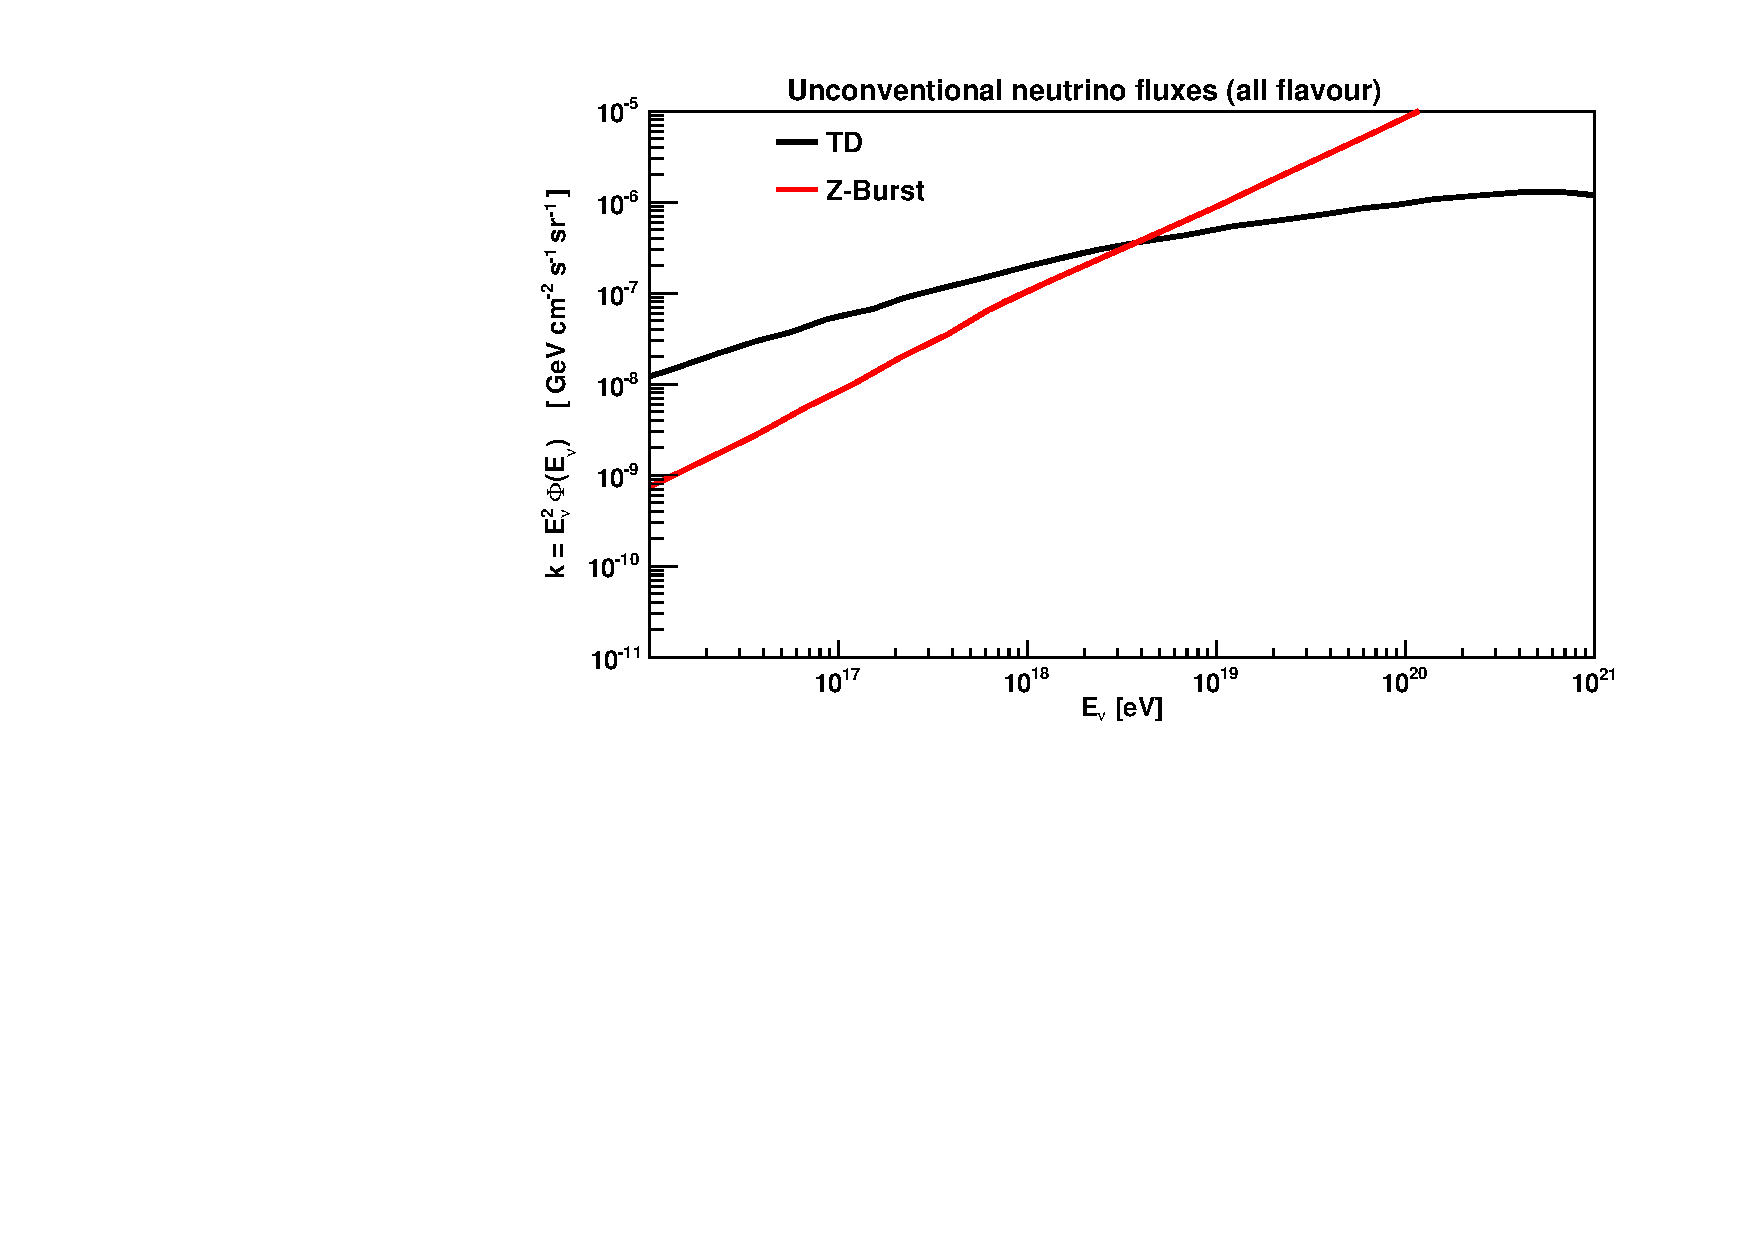
\includegraphics[width=0.75\textwidth]{fig/introduccion/unconventional_nuFluxes}
% 		\caption{\label{fig:flujosNoConv} }
% 		\end{center}
% 	\end{figure}

%\section{Búsquedas de neutrinos cósmicos UHE}
\section{Situación experimental}

En la actualidad existen diversos experimentos que desarrollan b\'usquedas de neutrinos c\'osmicos ultra energ\'eticos. 
En \cite{cite:nuSearchReview1} puede encontrarse una revisión detallada de los mismos as\'i como el estado de avance. 
En todos los casos se utiliza un blanco masivo con el que interact\'uan los neutrinos incidentes y se busca medir los efectos de tal interacci\'on.
En particular, el blanco puede consistir en agua, hielo, el aire de la atm\'osfera terrestre, la corteza terrestre o incluso grandes dep\'ositos naturales de sal.
En cuanto a la detecci\'on propiamente dicha, existen varias t\'ecnicas implementadas, como por ejemplo detectores \'opticos, de radio y de part\'iculas.

	\subsection{Detectores \'opticos}
	Las part\'iculas generadas en la interacci\'on entre neutrinos ultra energ\'eticos y medios densos viajan usualmente a velocidades superiores a la de la luz en dicho medio.
	Por ende, si el medio es transparente la luz \cher{} generada en este proceso puede ser capturada mediante fotomultiplicadores.
	
	A finales de los 90's el experimento pionero en esta t\'ecnica fue NT-200~\cite{cite:nt200}, un detector conformado por 192 m\'odulos \'opticos ubicados a \cant{\sim 1}{km} de profundidad en el lago Baikal, en Siberia.
	Sensible a neutrinos entre \cant{10^{14}\ {\text y}\ 10^{17}}{eV}, colectó datos durante casi una d\'ecada, imponiendo una cota superior al flujo de neutrinos de \cant{2\times 10^{-7}}{cm^{-2}s^{-1}sr^{-1}GeV}
	
	En la actualidad, el experimento de punta en la b\'usqueda de neutrinos c\'osmicos es IceCube~\cite{cite:IceCube1}.
	Este detector consiste en 5160 sensores \'opticos esf\'ericos, compuestos cada uno por 10 fotomultiplicadores, enterrados bajo el hielo polar ant\'artico a una profundidad entre \cant{1450}{m} y \cant{2450}{m}, cubriendo un volumen total de alrededor de \cant{1}{km^3}.
	La distribuci\'on de los detectores permite la detecci\'on de neutrinos con energ\'ias entre \cant{10^{11}}{eV} y \cant{10^{20}}{eV}.
	
	El arreglo subterráneo se encuentra tomando datos desde 2008 y es completamente operacional desde finales de 2010. 
	Una vez completo, ha observado eventos iniciados por neutrinos con energ\'ias sin precedentes (\cant{\geq 1}{PeV}), a una tasa de uno por a\~no.
	Recientemente se ha reportado el m\'as energ\'etico medido hasta el momento~\cite{cite:iceCubeEvent} con una energ\'ia de \cant{2.6\pm0.3}{PeV}.
	En conjunto, y habiendo descartado fuentes atmosf\'ericas por $6.5\,\sigma$, estos eventos representan definitivamente el descubrimiento de los neutrinos c\'osmicos.
	El mejor ajuste para un flujo de la forma $E^{-2}$, compatible con el mecanismo de aceleraci\'on de Fermi de primer orden resulta \cant{E^{-2}\phi(E) = (0.95\pm0.3)\times10^{-8}}{GeV\,cm^{-2}\,cm^{-1}\,sr^{-1}}\cite{cite:multimess}.
	Si bien su fuente es todav\'ia un misterio, estudios sobre la direcci\'on de arribo han sido compatibles con un flujo isotr\'opico, lo que sugiere la existencia de numerosas fuentes.
	Hasta la fecha IceCube no ha detectado neutrinos ultra energ\'eticos, o sea compatibles con origen cosmog\'enico.
	
	Otros experimentos que utilizan esta t\'ecnica son ANTARES~\cite{cite:Antares1}, NEMO~\cite{cite:Nemo1} y NESTOR~\cite{cite:Nestor1}, ubicados en diferentes puntos del Mar Mediterraneo.
	Aunque estos tres experimentos complementan la exposici\'on de IceCube observando el hemisferio norte, el volumen instrumentado no es lo suficientemente grande como para observar neutrinos ultra energ\'eticos.
	Para resolver esta limitaci\'on, KM3NeT~\cite{cite:km3Net1} instrumentar\'a alrededor de \cant{1}{km^3} bajo las aguas del Mediterr\'aneo.
	
	\subsection{Detectores de radio}
	A energ\'ias por encima de los \cant{10^{18}}{eV} el flujo de neutrinos c\'osmicos predicho por los diferentes modelos resulta demasiado peque\~no para  detectores del orden del $\rm km^3$. 
	Una t\'ecnica que permite sortear este obst\'aculo de manera efectiva es la detecci\'on de las ondas de radio generadas por efecto Askaryan en la cascada de part\'iculas subsiguiente a la interaci\'on. Este fenómeno, propuesto por Gurgen Askaryan a principios de los 60~\cite{cite:Askaryan} se basa que en que las part\'iculas de la lluvia producida por la interacci\'on del neutrino con el medio material dan lugar una carga efectiva en movimiento, que genera emisi\'on \cher{} en frecuencias de hasta el $\rm GHz$.
	Incluso en medios densos como hielo, sal o arena, a estas frecuencias la longitud de atenuaci\'on puede rondar los cientos de metros.
	Si adem\'as se tiene en cuenta el bajo costo relativo de los detectores de radio (frente a por ejemplo fotomultiplicadores) resulta evidente que esta t\'ecnica tiene potencial en detectores de gran tama\~no.
	A continuaci\'on se realiza un recuento de los experimentos pasados, actuales y futuros que utilizan esta t\'ecnica:
	
	\textbf{RICE} (Radio Ice Cherenkov Experiment): realiz\'o la b\'usqueda en base a la emisi\'on producida por cascadas electromagn\'eticas y hadr\'onicas inducidas por la interacci\'on de UHE$\nu$'s en el hielo ant\'artico.
	Este experimento consisti\'o en un arreglo de 16 antenas, cuyo ancho de banda abarc\'o los 200-1000~MHz, ubicadas en un cubo de \cant{200}{m} de lado a \cant{150}{m} de profundidad cerca del polo sur.
	En base a los datos colectados entre 1999 y 2005, luego de no haber detectado ning\'un evento candidato,
RICE impuso un l\'imite superior al flujo de neutrinos c\'osmicos de todos los sabores (All Flavor) dado por
	 %
	\begin{equation}
	 E^{-2}\phi_\nu \leq 10^{-6}{\rm\ GeV\,cm^{-2}s^{-1}sr^{-1}}
	\end{equation}
	 %
	en un rango energ\'etico entre \cant{10^{17}}{eV} y \cant{10^{20}}{eV}~\cite{cite:RICE}.
	 
	\textbf{ANITA} (Antartic Impulsive Transient Array): este experimento fue lanzado por NASA desde la estaci\'on McMurdo. 
	Consiste en un detector conformado por un arreglo de 32 antenas tipo bocina, sensibles en el rango de 200\-1200~MHz, y transportado en un globo atmosf\'erico hasta los \cant{37}{km} de altitud sobre el suelo ant\'artico.
	Luego del prototipo ANITA-LITE en 2004, se lanzó en 2006 el detector completo, que se mantuvo en vuelo durante 35 d\'ias~\cite{cite:Anita1}.
	 
	Un segundo vuelo, en 2008, cont\'o con 8 antenas m\'as en el detector y una mejora en la electr\'onica.
	Luego de 28.5 d\'ias m\'as en el aire y habiendo tenido un evento candidato finalmente clasificado como fondo, ANITA-II impuso una cota superior (\cant{90\%}{CL}) al flujo de neutrinos de:
	 %
	\begin{equation}
	 E^{-2}\phi_\nu \leq 1.3\times10^{-7}{\rm\ GeV\,cm^{-2}s^{-1}sr^{-1}}
	\end{equation}
	 %
	en el rango de energ\'ias de \cant{10^{18}}{eV} a \cant{10^{23.5}}{eV}~\cite{cite:Anita2}.
	
	\textbf{GLUE} (Goldstone Lunar Ultrahigh Energy) realiz\'o una b\'usqueda de pulsos de microondas en el rango de los \cant{10}{\mu s} provenientes del suelo lunar en coincidencia con pulsos de radio. 
	Tales pulsos emerger\'ian de cascadas electromagn\'eticas desarrolladas en el interior de la masa lunar, producidas por la interacci\'on de UHE$\nu$'s. 
	Luego de 30 horas efectivas de observaci\'on y ningún candidato observado, GLUE estableci\'o una cota superior al flujo de neutrinos entre \cant{10^{19}}{eV} y \cant{10^{22.5}}{eV}~\cite{cite:Glue}.
	Anteriormente, los experimentos Kalyazin \cite{cite:Kalazin} y Parkes \cite{cite:Parkes} ya hab\'ian realizado b\'usquedas de se\~nales provenientes de la luna tambi\'en sin resultados positivos.
	Por otra parte, existen otros experimentos que pretenden explotar esta t\'ecnica, como el radio telescopio NuMoon~\cite{cite:NuMoon}, el futuro Square Kilometer Array (SKA)~\cite{cite:SKA}, o LUNASKA (Lunar UHE Neutrino Astrophysics using the Square Kilometer Array)~\cite{cite:LUNASKA}.
	
	\textbf{ARA} (Askaryan Radio Array): actualmente en construcci\'on, ARA se ubica cerca del polo sur geogr\'afico, cerca de IceCube~\cite{cite:ARA}.
	Su dise\~no le permite detectar la interacci\'on de neutrinos GZK en la corteza de hielo de la Ant\'artida, contando as\'i con un blanco que abarca miles de kil\'ometros cuadrados de superficie por \cant{3}{km} de profundidad.
	Para ello, ARA desplegar\'a 37 clusters de antenas, separadas por \cant{2}{km} en una grilla hexagonal, distancia que maximiza la sensitividad a \cant{10^{18}}{eV}, e instalados a \cant{200}{m} de profundidad en el hielo.
	Actualmente se encuentran instaladas tres estaciones, de las cuales dos han tomado datos desde finales de 2013~\cite{cite:ARA2}.
	
	\textbf{ARIANNA} (Antartic Ross Ice-Shelf ANtenna Neutrino Array): este detector pretende usar el escudo de Ross en la costa ant\'artica como blanco para neutrinos GZK por encima de los \cant{10^{17.5}}{eV}~\cite{cite:ARIANNA}.
	Este detector surgi\'o de estudios recientes~\cite{cite:ARIANNA2} que determinaron que el fondo del casquete de hielo que conforma el escudo de Ross posee buenas propiedades de reflectividad de ondas de radio.
	El detector completo estar\'a constituido en un arreglo cuadrado de $36\times36$ estaciones, cada una constando de ocho antenas bajo el hielo, en un arreglo octogonal, y dos sobre la superficie.
	El objetivo de estas antenas es detectar las ondas de radio generadas por las cascadas electromagn\'eticas subsiguientes a la interacci\'on de los neutrinos en el hielo. Dado que estas ondas pueden ser reflejadas en la interface hielo agua sobre el fondo del casquete, ARIANNA tambien es sensible a neutrinos descendentes.
	Como prueba de concepto se utilizar\'a una estaci\'on de prueba de 6 antenas de las cuales 3 tomaron datos en 2013 y 2014~\cite{cite:ARIANNA3}.
	
	\textbf{GRAND} (Giant Radio Array for Neutrino Detection) es una propuesta para construir un arreglo de antenas de superficie \cant{>50000}{km^2}, que planea detectar neutrinos en el rango del\cant{}{EeV}. 
	La disposici\'on preliminar consiste en la ubicaci\'on de $\sim90000$ unidades de detecci\'on desplegadas en una grilla cuadrada de \cant{800}{m} de paso ubicado en el cordon monta\~noso de Tianshan, China.
	Cada unidad de detecci\'on se compondr\'a de un sistema de adquisici\'on y de tres antenas tipo mariposa orientadas de manera perpendicular, lo que permitir\'a una medici\'on completa de la polarizaci\'on del campo el\'ectrico. 
	Actualmente se encuentran instaladas 35 estaciones de prueba junto con un arreglo de 20 centelladores con el fin de realizar un chequeo cruzado entre detectores y estimar el desempe\~no del detector de prueba.
	Estimaciones preliminares predicen en tres a\~nos de medici\'on una mejora de casi dos \'ordenes de magnitud respecto de los l\'imites actuales.
	
	ARA, ARIANNA y GRAND prometen entregar las mediciones m\'as sensibles de la pr\'oxima generaci\'on de detectores de neutrinos ultra energ\'eticos.

% 
% 		\begin{figure}[ht]
% 		\begin{center}
% 		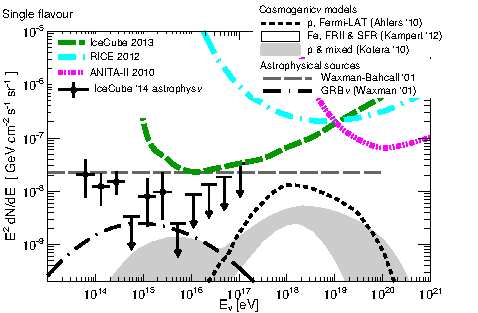
\includegraphics[width=0.75\textwidth]{fig/introduccion/1510-02050_multimessenger_noAuger}
% 		\caption{\label{fig:multimess}  Flujo de neutrinos medido por el experimento IceCube (datos), junto con los distintos límites superiores impuestos por Anita-II, IceCube y Rice. Tambi\'en se muestran los flujos esperados para varios modelos cosmog\'enicos, as\'i como la cota de Waxman-Bahcall. Figura tomada de \cite{cite:multimess}.}
% 		\end{center}
% 	\end{figure}

	\subsection{Detectores de rayos c\'osmicos}
	
	Los experimentos de rayos c\'osmicos tambien son sensibles al flujo de neutrinos c\'osmicos ultra energ\'eticos. 
	Dado que son dise\~nados para detectar las lluvias atmosf\'ericas iniciadas por UHECRs, tienen la capacidad de medir las generadas por neutrinos en la atm\'osfera as\'i como los que interact\'uan en la corteza terrestre.
	En al actualidad, la delantera entre este tipo de experimentos la lleva el Observatorio Pierre Auger, y dentro de este proyecto se enmarca el presente trabajo. 	
	%
	%El observatorio realiz\'o una b\'usqueda de neutrinos con energ\'ias cercanas al \cant{1}{EeV} entre los eventos detectados con el SD.  El estudio se encuentra dividido en tres sub an\'alisis optimizados para detectar neutrinos en distintos rangos angulares: de $60^\circ$ a $75^\circ$, de $75^\circ$ a $90^\circ$ y de $90^\circ$ a $95^\circ$, siendo estos \'ultimos eventos iniciados por \nutau{} que interact\'uan contra la corteza terrestre y producen un \tauon{} que inicia una lluvia atmosf\'erica ascendente cerca del detector. El trabajo original  





	%%%%%%%%%%%%%%%%%%%%%%%%%%%%%%%%%%%%%%%%%%%%%%%%%%%%%%%%%%%%%%%%%%%%%%%
	\if{0} % Esto no va, la descripcion del detector es el proximo capitulo
	%%%%%%%%%%%%%%%%%%%%%%%%%%%%%%%%%%%%%%%%%%%%%%%%%%%%%%%%%%%%%%%%%%%%%%%
	El detector se encuentra ubicado en la provincia de Mendoza, Argentina a una altitud de \cant{1400}{m} (profundidad atmosf\'erica de \cant{875}{g\,cm^{-2}}).
	Este consta de un sistema h\'ibrido de detecci\'on que combina un detector de superficie (SD) de tama\~no sin precedes y un conjunto de telescopios de fluorescencia (FD).
	El SD se compone de 1660 estaciones \cher{} ubicadas en una grilla triangular de \cant{1500}{m} de paso desplegada sobre una superficie de \cant{3000}{km^2}, mientras que los 27 telescopios del FD observan la atm\'osfera sobre el SD desde 4 estaciones a su alrededor.
	\fi %%%%%%%%%%%%%%%%%%%%%%%%%%%%%%%%%%%%%%%%%%%%%%%%%%%%%%%%%%%%%%%%%%%%%%%%%


	%%%%%%%%%%%%%%%%%%%%%%%%%%%%%%%%%%%%%%%%%%%%%%%%%%%%%%%%%%%%%%%%%%%%%%%%%
	\if{0} % 
	El observatorio realiz\'o una b\'usqueda de neutrinos con energ\'ias cercanas al \cant{1}{EeV} entre los eventos detectados con el SD.
	Mientras que los rayos c\'osmicos regulares (protones, n\'ucleos pesados y fotones) interact\'uan cerca del tope de la atm\'osfera, los neutrinos tienen la capacidad de iniciar lluvias atmosf\'ericas extendidas muy cerca del detector. 
	Cuando el \'angulo cenital es grande ($>60^\circ$) la componente electromagn\'etica de las lluvias de origen hadr\'onico es absorbida debido al espesor m\'asico de la atm\'osfera (alcanzando los \cant{\sim30000}{g\,cm^{-2}} a $\theta\sim90^\circ$), provocando que s\'olo la componente mu\'onica alcance la superficie de la Tierra.
	Por otra parte, las lluvias inducidas por neutrinos, iniciadas profundo en la atm\'osfera tendr\'an una fuerte presencia de componente electromagn\'etica al interactuar con el detector.
	De esta manera, la b\'usqueda se realiza discriminando eventos que presenten esta componente entre los inclinados. 
	
	Actualmente el an\'alisis del observatorio se encuentra dividido en tres sub an\'alisis optimizados para detectar neutrinos en distintos rangos angulares: de $60^\circ$ a $75^\circ$, de $75^\circ$ a $90^\circ$ y de $90^\circ$ a $95^\circ$, siendo estos \'ultimos eventos iniciados por \nutau{} que interact\'uan contra la corteza terrestre y producen un \tauon{} que inicia una lluvia atmosf\'erica ascendente cerca del detector.
	Luego de un escrutinio realizado sobre los datos tomados entre el 1 de enero de 2004 y el 20 de junio de 2013 no fue hallado ning\'un evento candidato, imponiendo una cota superior al flujo con un \cant{90\%}{CL} de~\cite{Aab:2015kma}:
	 %
	\begin{equation}
	 E^{-2}\phi_\nu \leq 6.4\times10^{-9}{\rm\ GeVcm^{-2}s^{-1}sr^{-1}}
	\end{equation}
	%
	en un rango energ\'etico que comprende \cant{1.0\times10^{17}}{eV} a \cant{2.5\times10^{19}}{eV}.
	Es importante remarcar que este es el primer experimento de rayos c\'osmicos que supera la cota de Waxman-Bahcall
	\fi 
	%%%%%%%%%%%%%%%%%%%%%%%%%%%%%%%%%%%%%%%%%%%%%%%%%%%%%%%%%%%%%%%%%%%%%%%%%


	
	%%%%%%%%%%%%%%%%%%%%%%%%%%%%%%%%%%%%
        \if{0}  % ESTO VA A LAS CONCLUSIONES
        %%%%%%%%%%%%%%%%%%%%%%%%%%%%%%%%%%%%
	\subsection{Panorama actual en la b\'usqueda de neutrinos c\'osmicos ultra energ\'eticos}
	
	Se han detectado por primera vez neutrinos c\'osmicos de alta energ\'ia, sin embargo, hasta el momento su origen sigue siendo un misterio.
	La figura \ref{fig:multimess} muestra el estado actual de la detecci\'on, combinando el flujo medido en el PeV por IceCube, los l\'imites diferenciales más estrictos impuestos hasta el momento por Auger, IceCube, RICE y ANITA-II, y algunos flujos cosmog\'enicos.
	%
	
	Tanto IceCube como Auger han alcanzado exposiciones sin precedentes, lo que ha permitido descartar los modelos de AGN y los cosmog\'enicos m\'as optimistas, mientras que el resto de los que suponen protones como primario comienzan a verse desfavorecidos.
	Por otro lado, los que utilizan una componente primaria m\'as pesada se encuentran todav\'ia lejos del alcance de la detecci\'on actual.
	Por \'ultimo, una extrapolaci\'on del mejor ajuste del flujo medido por IceCube al rango de observaci\'on de Auger predice 0.1 eventos en su \'ultimo per\'iodo de medici\'on, compatible con una observaci\'on de 0 candidatos.
	
	Queda claro entonces que la nueva generaci\'on de detectores de neutrinos tiene mucho por descubrir.
	La observaci\'on del corte GZK respalda la existencia de un flujo cosmog\'enicos pero resultados recientes de Auger indican una migraci\'on hacia una componente m\'as pesada en los eventos de alta energ\'ia, lo que implicar\'ia flujos de neutrinos m\'as peque\~nos.
	Por este motivo la llegada de ARA, ARIANNA y GRAND generan mucha espectativa dentro de la comunidad.
	\fi %%%%%%%%%%%%%%%%%%%%%%%%%%%%%%%%%%%%

% 	Esta tesis se encuentra dedicada al estudio de la detecci\'on de neutrinos c\'osmicos con detectores de superficie. 
% 	En la primer parte se presenta la b\'usqueda de neutrinos c\'osmicos realizada con el Observatorio Pierre Auger entre enero de 2004 y junio de 2013.
% 	Se describir\'a en detalle cada uno de los an\'alisis, los m\'etodos empleados en la discriminaci\'on de eventos candidatos y el c\'alculo de la exposici\'on, presentando por primera vez un resultado combinado, que dio lugar al l\'imite m\'as estricto publicado por Auger hasta la fecha.
% 	En la segunda parte se estudian las capacidades y limitaciones de un arreglo de antenas de radio al detectar neutrinos ultra energ\'eticos.
% 	Mediante simulaciones Monte Carlo se analiz\'o la factibilidad de la detecci\'on y se calcul\'o la exposici\'on que podr\'ia alcanzar un detector de las caracter\'isticas de GRAND.
% 	
	

\part{Detecci\'on de neutrinos ultra energ\'eticos con el observatorio Pierre Auger}
\chapter{El Observatorio Pierre Auger}
\label{ch:detectorAuger}

El objetivo del Observatorio Pierre Auger es colectar eventos de rayos c\'osmicos con energ\'ias mayores a $10^{18}\ eV$, con el fin de comprender su naturaleza. En particular, se busca reconstruir el espectro energ\'etico con precisi\'on sin precedentes, medir las direcciones de arribo y estudiar la composici\'on de los mismos. El Observatorio se encuentra en Pampa Amarilla a una altitud promedio de $\sim 1400\ m$, cerca de Malarg\"ue, en la provincia de Mendoza, Argentina.
\'Este lugar fue elegido debido a que el terreno es relativamente plano, variando menos de $200\ m$ en toda la extensi\'on del observatorio, y el clima \'arido con cielos despejados. 

	\section{Descripción general}
	Este detector combina las fortalezas de dos t\'ecnicas de detecci\'on: una grilla triangular de 1600 detectores Cherenkov (detector de superficie o SD) y 4 detectores de fluorescencia (detector de fluorecencia o FD).
	El detector h\'ibrido tiene importantes ventajas sobre cada una de las t\'ecnicas operando por separado, ya que observar lluvias en simult\'aneo permite identificar las fuentes de incertezas sistem\'aticas de cada t\'ecnica y medir independientemente propiedades de la lluvia.
	Las ventajas principales del detector de superficie son que puede operar el $100 \%$ del tiempo, su respuesta es poco dependiente del clima, su apertura se encuentra bien definida y es independiente de la energ\'ia por encima de $10^{19}\ eV$, su se\~nal puede autocalibrarse usando muones de rayos c\'osmicos  y tiene una alta sensitividad a lluvias que lleguen con grandes \'angulos cenitales. 
	Pero un experimento que s\'olo conste de un SD no podr\'ia realizar una reconstrucci\'on en energ\'ia sin asumir qu\'e part\'icula inici\'o la lluvia y una simulaci\'on de por medio~\cite{busca_thesis}.
	Por otro lado, el detector de fluorescencia posee la ventaja de medir directamente el perfil longitudinal de las EAS y poder realizar una medici\'on calorim\'etrica de la energ\'ia, sin necesidad de simulaciones. Pero la desventaja de este detector es que s\'olo puede realizar mediciones en noches sin luna y sin nubes, aproximadamente un $10 - 15 \%$ del tiempo de medici\'on.
	
	Al combinar ambas t\'ecnicas de medici\'on, es posible realizar una calibraci\'on cruzada entre ambos detectores, que permite calibrar en energ\'ia el SD sin ninguna suposici\'on sobre la part\'icula incidente.
	De hecho, se observa una correlaci\'on entre el tama\~no de la lluvia en el SD y la energ\'ia reconstruida con el FD.
	Al mismo tiempo, los eventos observados por ambos detectores tienen una mejora significativa en la reconstrucci\'on de la geometr\'ia de la lluvia y la energ\'ia de la misma.
	
	En la figura \ref{fig:plano_auger} se observa la disposici\'on geom\'etrica del detector.
	Los puntos negros corresponden a los detectores Cherenkov, separados por $1.5\ km$ en un arreglo triangular.
	Tambi\'en se observan los 4 detectores de fluorecencia, cada uno con 6 telescopios, cuya direcci\'on de observaci\'on se denota con lineas negras.
	
	\begin{figure}[h!]
		\begin{center}
		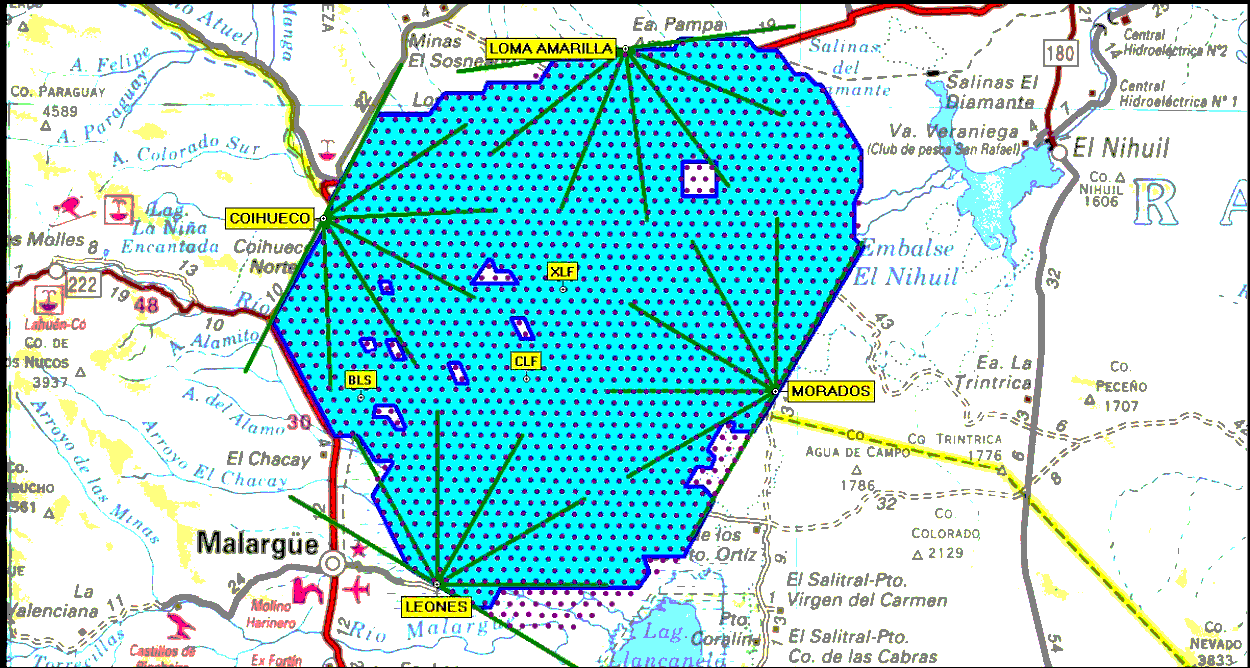
\includegraphics[width=\textwidth]{fig/detectorAuger/array}
		\caption{\label{fig:plano_auger} Ubicaci\'on geogr\'afica del Observatorio Pierre Auger. Los puntos negros dentro del \'area turquesa representan los tanques en funcionamiento a finales de 2009. 
		Las l\'ineas verdes indican el campo de visi\'on de cada uno de los 6 telescopios de cada detector de fluorecencia.}
		\end{center}
	\end{figure}
	
	Los eventos registrados se clasifican de la siguiente manera:
	\begin{itemize}
		\item Eventos SD: s\'olo detectados por la grilla de superficie.
		\item Eventos FD:
		\begin{itemize}
			\item Mono: s\'olo un detector de fluorescencia lo observa
			\item Stereo: lo observan 2 o m\'as detectores de fluorescencia 
		\end{itemize} 
		\item Eventos H\'ibridos:
		\begin{itemize}
			\item Simple: 1 detector FD + 1 tanque SD o algunos tanques SD, pero no suficientes como para hacer una reconstrucci\'on independiente SD.
			\item Dorados: 1 detector FD + $n$tanques SD, con $n$ suficientemente grande como para hacer una reconstrucci\'on SD independiente.
			\item Platino: 2 o m\'as detectores FD + cualquier informaci\'on del SD.
		\end{itemize}
	\end{itemize}
	
	\section{Detector de superficie}
	
	El detector de superficie del Observatorio Pierre Auger consta de 1600 tanques Cherenkov ubicados en un arreglo hexagonal, en el que cada tanque se encuentra a $1.5\ km$ de sus 6 vecinos, cubriendo en total una superficie de $3000\ km^2$.
	
	El objetivo de cada unidad del detector es colectar la radiaci\'on Cherenkov emitida por las part\'iculas que pasan por su interior.
	Cada una consiste de un tanque cil\'indrico de polietileno de $3.6\ m$ de di\'ametro y $1.55\ m$ de alto, cubriendo un {\em liner} repleto de 12 toneladas de agua excepcionalmente pura. 
	El {\em liner} es un bolsa pl\'astica cil\'indrica de $1.2\ m$ de altura, que es negra por fuera para sellarla de luz externa mientras que dentro est\'a protegida con Tyvek para reflejar la luz Cherenkov. 
	La luz Cherenkov es colectada por tres fototubos de 8 pulgadas cada uno, y su señal es continuamente registrada por un convertidor anal\'ogico digital (FADC) en bines de $25\ ns$.
	Esta se\~nal es muestreada con una frecuencia de $40\rm \ MHz$ y una resoluci\'on de 10 bits mediante un CPU, que tambi\'en realiza las primeras decisiones de trigger.
	Cada estaci\'on est\'a equipada, adem\'as, con un GPS que permite sincronizar los relojes de todas las estaciones con una precisi\'on de $8\rm \,ns$ \cite{auger_prop04}.
	En la figura \ref{fig:tanque} se muestra una foto de un tanque ya instalado seguido de un esquema que especifica cada una de sus partes.
	
	Puesto que muchas veces la zona donde se encuentra el tanque es de dif\'icil acceso, \'estos fueron diseñados para ser unidades aut\'onomas equipadas con un panel solar, bater\'ias y una antena de comunicaci\'on.
	Las trazas de los fototubos y los datos de tiempo son almacenados por la estaci\'on en un buffer que es posteriormente transmitido a una computadora central en el centro de adquisici\'on de datos (CDAS).
	
	\begin{figure}[h!]
		\begin{center}
		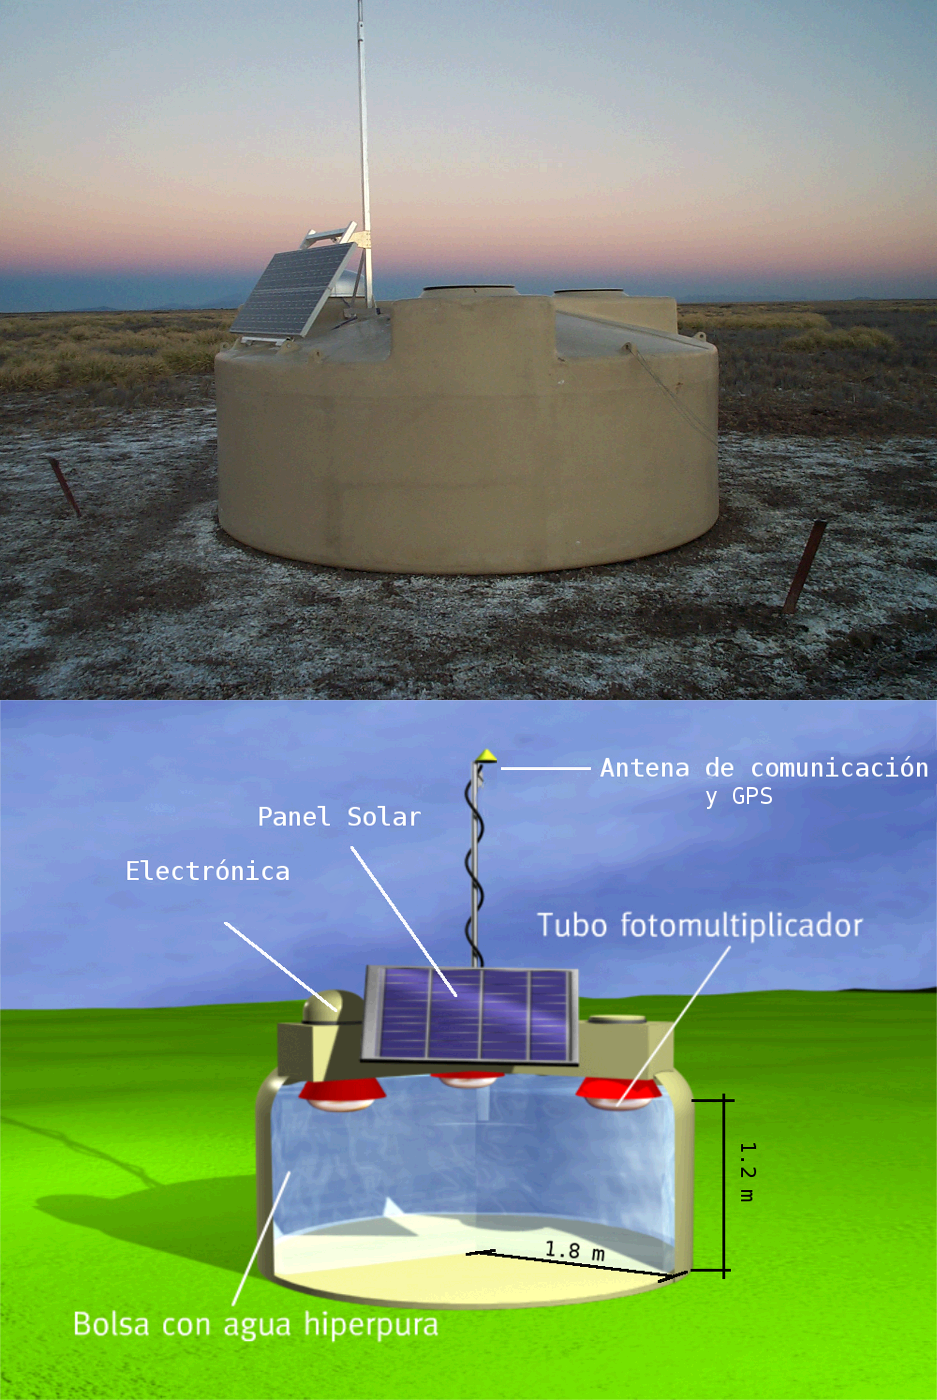
\includegraphics[width=0.7\textwidth]{fig/detectorAuger/Tanque00}
		\caption{\label{fig:tanque} En la parte superior (inferior) de la figura se muestra una foto (esquema) de uno de los tanques del arreglo de superficie del Observatorio Pierre Auger, en Malarg\"ue.}
		\end{center}
	\end{figure}

		\section{Calibraci\'on del detector de superficie}
		
		La Colaboraci\'on Auger ha adoptado al VEM (Vertical Equivalent Muon) como unidad de medida para las señales adquiridas por el SD.
		El VEM se define como la señal promedio producida en un tanque del SD al ser atravesado por su eje por un mu\'on vertical.
		
		Dada la gran cantidad de estaciones y la dificultad de acceder a ellas, el proceso de calibraci\'on implementado en el SD es realizado de manera aut\'onoma por la computadora de cada tanque. 
		Los muones atmosf\'ericos tienen una frecuencia de arribo uniforme sobre todo el detector lo que los hace ideales para lograr una buena calibraci\'on relativa entre los tanques. 
		Es por ello que el algoritmo de calibraci\'on implementado se basa en la medici\'on de su espectro. 
		La figura \ref{Calibracion_Muones} muestra un espectro t\'ipico adquirido por uno de los tanques. 
		A partir de experiencias realizadas utilizando un tanque en conjunci\'on con un telescopio de muones se ha determinado que el segundo\footnote{El primero es consecuencia del diseño de la electrónica.} pico corresponde a \cant{1.05}{VEM}. 
		Utilizando esta referencia cada tanque ajusta su ganancia de manera tal que coincida con la de los dem\'as.
		
		\begin{figure}[ht]
			\begin{center}
			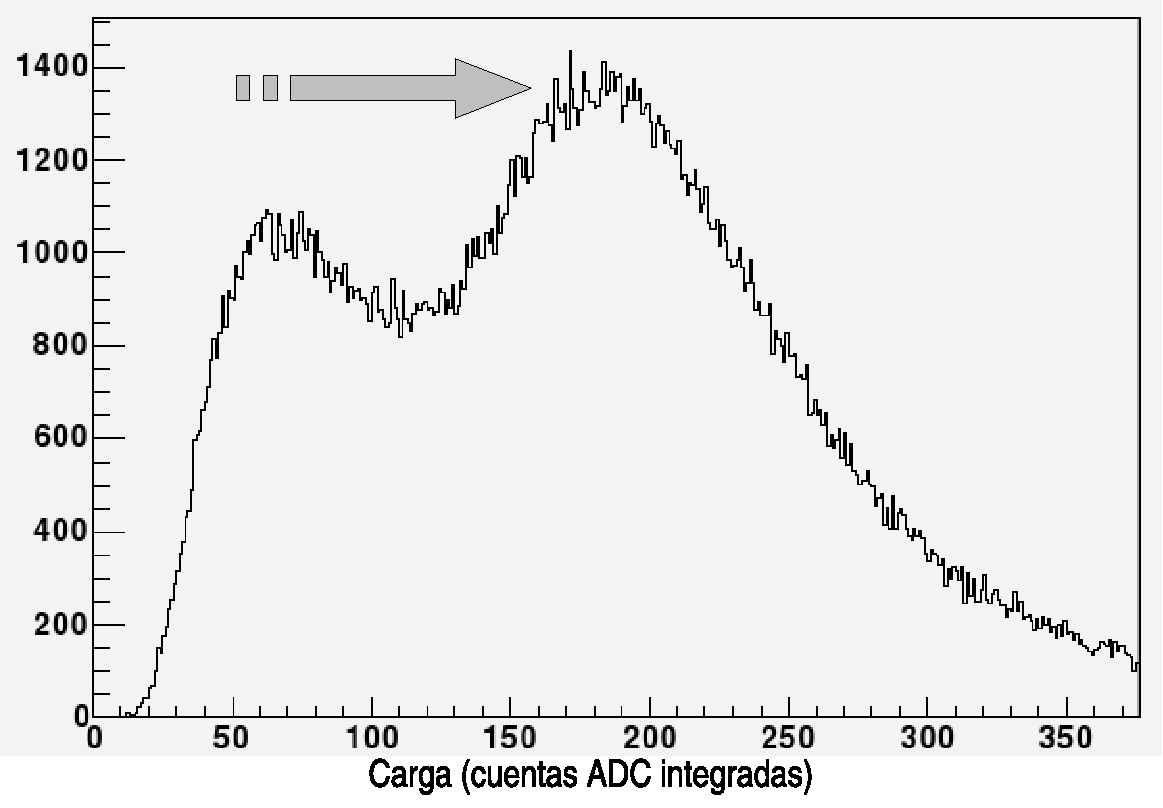
\includegraphics[width=0.8\textwidth]{fig/detectorAuger/vem}
			\caption{Espectro de muones atmosf\'ericos para una coincidencia de tres fototubos. El pico se\~nalado corresponde a \cant{1.05}{VEM}}
			\label{Calibracion_Muones}
			\end{center}
		\end{figure}
		
		
		\section{Disparo del detector de superficie}
		\label{sbsc:trig_levels}
		
		Con el fin de limitar la cantidad de eventos almacenados y minimizar la contaminaci\'on, el Proyecto Auger ha adoptado una estructura jer\'arquica de disparos para el detector de superficie, que puede clasificarse b\'asicamente en dos niveles \cite{icrctri}:
		
		\begin{shortitemize}
		\item Trigger de bajo nivel
		\item Trigger de alto nivel
		\end{shortitemize}
		
			\subsection*{Trigger de bajo nivel}
			
			Este nivel de trigger se aplica en tiempo real en cada estaci\'on con dos fines, disminuir la frecuencia de detecci\'on de muones atmosf\'ericos y distinguir entre las componentes mu\'onicas y electromagn\'eticas de la lluvia.
			Aqu\'i la nomenclatura utilizada \cite{nimtrig}:
			
			\begin{itemize}
			\item T1-Threshold (T1-TH): Corresponde a una traza que supera \cant{1.75}{VEM} en los tres PMT's del taque. El objetivo principal de este criterio es disminuir de \cant{\approx3}{kHz} a \cant{\approx 100}{Hz} la detecci\'on de muones atmosf\'ericos.
			\item T1-Time Over Threshold (T1-ToT): Corresponde a una se\~nal que supera \cant{0.2}{VEM} en m\'as de 13 bines de FADC dentro de una ventana de 120 bines (\cant{3}{\mu s}), para dos cualesquiera de los 3 PMT's. Este criterio busca detectar lluvias con gran componente electromagn\'etica al nivel del suelo y la parte mas alejada de las lluvias verticales, debido a que la dispersi\'on temporal en el arribo de las part\'iculas al detector es grande (\cant{\approx 300}{ns} para un tanque que se encuentra a \cant{1000}{m} del eje en una lluvia vertical \cite{disp1,disp2}). La frecuencia de disparo de este nivel es \cant{\approx 1.6}{Hz}.
			\item T2-Threshold (T2-TH): Para cumplir esta categor\'ia se pide una traza que supere \cant{3.2}{VEM}. Este criterio baja la frecuencia de disparo de \cant{\approx 100}{Hz} a \cant{\approx 20}{Hz}.
			\item T2-Time Over Threshols (T2-ToT): Todos los T1-ToT pasan directamente a esta categor\'ia. %La frecuencia de aparicion de este tipo de disparo es \cant{\approx 1.6}{Hz}
			\end{itemize}
			
			En las figuras \ref{fig:t2_th} y \ref{fig:t2_tot} se muestran las trazas de los tres PMT's para eventos clasificados como T2-TH y T2-ToT respectivamente.
			
			\begin{figure}[h!]
				\begin{center}
				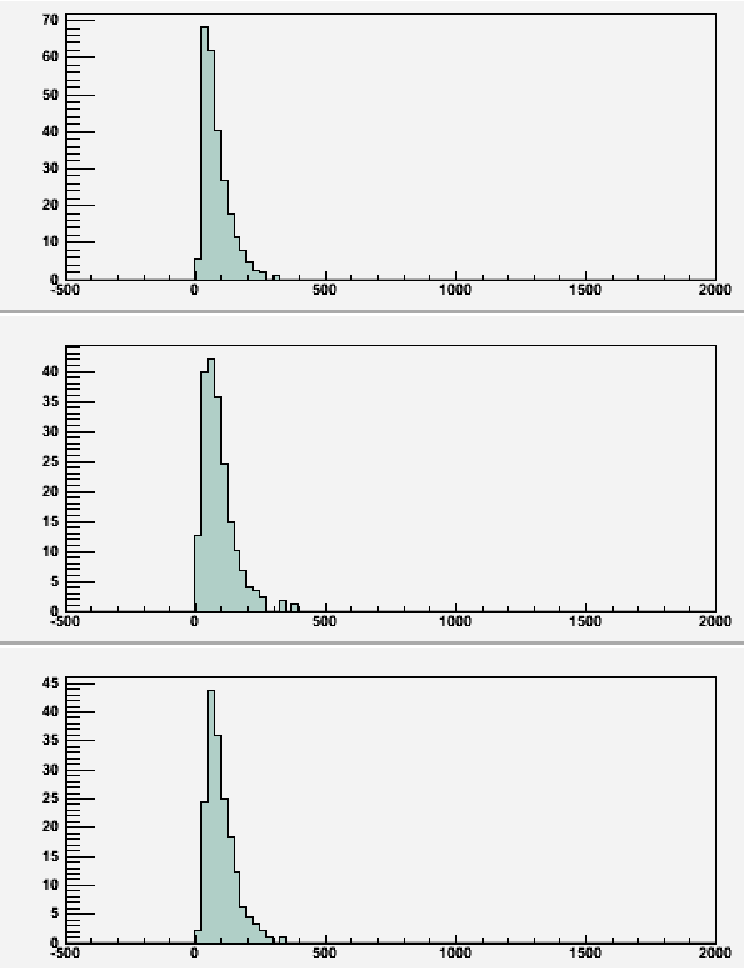
\includegraphics[width=0.45\textwidth]{fig/detectorAuger/Threshold}
				\caption{\label{fig:t2_th} Ejemplo de traza que produce un T2-Threshold.}
				\end{center}
			\end{figure}
			\begin{figure}[h!]
				\begin{center}
				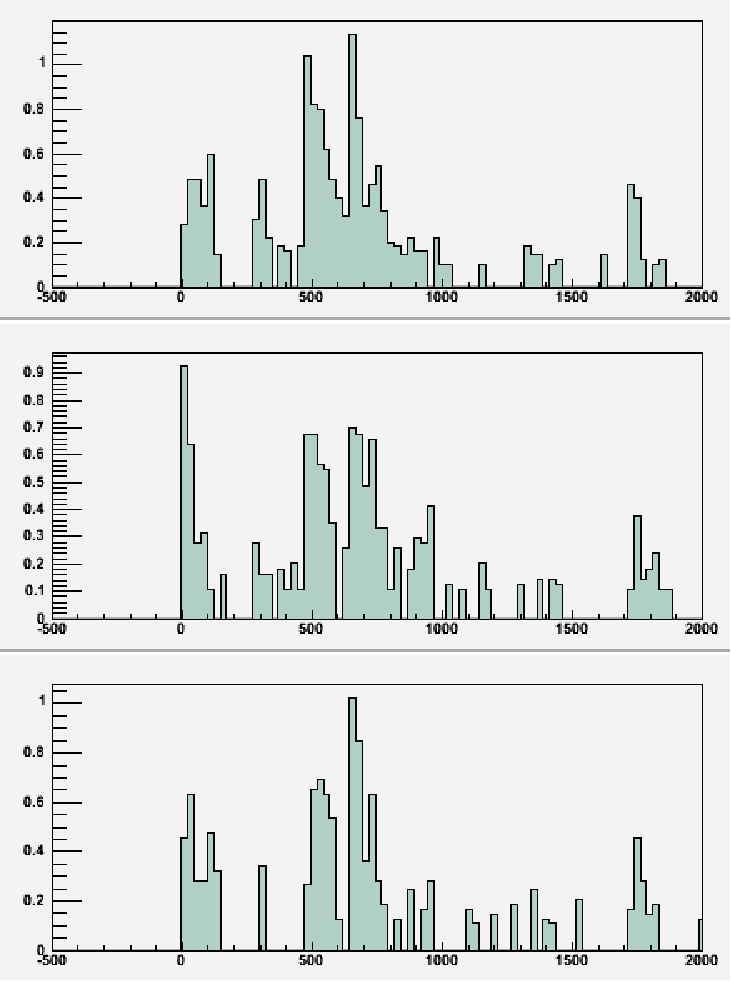
\includegraphics[width=0.45\textwidth]{fig/detectorAuger/ToT}
				\caption{\label{fig:t2_tot} Ejemplo de traza que produce un T2-ToT}
				\end{center}
			\end{figure}
			
			Todas las estaciones con T1 o T2 se guardan durante \cant{10}{s} esperando un posible trigger de m\'as alto nivel, T3.
			
			\subsection*{Trigger de alto nivel}
			
			\titulo{Trigger del detector T3} El siguiente nivel de trigger es T3, que es iniciado desde el CDAS seg\'un cierta combinaci\'on espacial y temporal de estaciones con T2.
			Una vez detectado un T3, son guardadas las trazas de todas las estaciones con T1 o T2 dentro de una ventana temporal de \cant{30}{\mu s}.
			El trigger del detector se realiza seg\'un dos categorias:
			
			\begin{itemize}
			\item 3ToT ($\rm ToT2C_1\&3C_2$): Este criterio requiere que al menos 3 detectores sean ToT. Tambi\'en requiere cierta compacticidad en la distribuci\'on espacial de la se\~nal, pidiendo que al menos dos tanques sean primeros vecinos y el tercero se encuentre en la segunda corona de alguno de los dos. La nomenclatura de esta categor\'ia es $\rm ToT2C_1\&3C_2$, donde $\rm C_n$ se refiere a la corona n-\'esima desde alguno de los tanques, siempre el mismo. En el panel izquierdo de la figura \ref{fig:coronas} se muestra una configuraci\'on de tanques que cumple con esta categor\'ia. Una vez satisfecho el criterio espacial, se somete la configuraci\'on a un criterio temporal, pidiendo que cada tanque se encuentre separado a menos de \cant{(6+5{\rm C_n})}{ns} del primero, donde $C_n$ indica en n\'umero de corona en el que se encuentra. Se registran del orden de 1600 de estos eventos por d\'ia, siendo el \cant{90}{\%} de estos eventos f\'isicos, debido al bajo nivel de contaminaci\'on que presentan los tanques con T2-ToT. El \cant{10}{\%} restante se debe al permisivo criterio temporal.
			\item 4 fold T2 ($\rm2C_1\&3C_2\&4C_4$): Este criterio es mucho menos exigente, pidiendo cuatro T2 con una compacticidad espacial moderada. Para satisfacer esta categor\'ia se pide que dos tanques sean primeros vecinos, que el tercero se encuentre dentro de la segunda corona de alguno de los dos y que exista al menos un tanque m\'as en la cuarta corona del anterior. Un ejemplo de esta distribuci\'on espacial se muestra en el panel derecho de la figura \ref{fig:coronas}. Tambi\'en se pide el mismo criterio temporal que para la categor\'ia $\rm ToT2C_1\&3C_2$. Este nivel de trigger tiene buena eficiencia para eventos inclinados, pero es muy sensible a disparos casuales de los tanques, por lo que de los 1200 eventos registrados diariamente, \cant{\approx 10}{\%} de ellos corresponden a lluvias reales.
			\end{itemize}
			
			\begin{figure}[h!]
				\begin{center}
				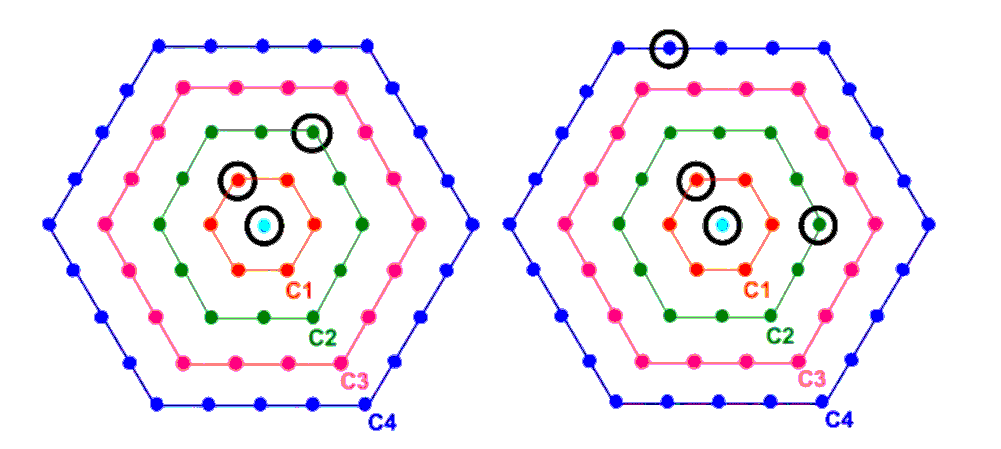
\includegraphics[width=\textwidth]{fig/detectorAuger/coronas}
				\caption{\label{fig:coronas} Ejemplos de configuraciones T3: en el panel izquierdo (derecho) se muestra un ejemplo una configuraci\'on que satisface el criterio $\rm ToT2C_1\&3C_2$ ($\rm 2C_1\&3C_4\&4C_4$). $\rm C_1$, $\rm C_2$, $\rm C_3$ y $\rm C_4$ indican la primera, segunda, tercera y cuarta corona de vecinos respectivamente, a 1.5, 3, 4.5 y 6 km para un dado detector.}
				\end{center}
			\end{figure}
			
			En la figura \ref{fig:diagtrig} se muestra la jerarqu\'ia de triggers hasta T3.
			\vspace{0.5cm}
			
			\begin{figure}[h!]
				\begin{center}
				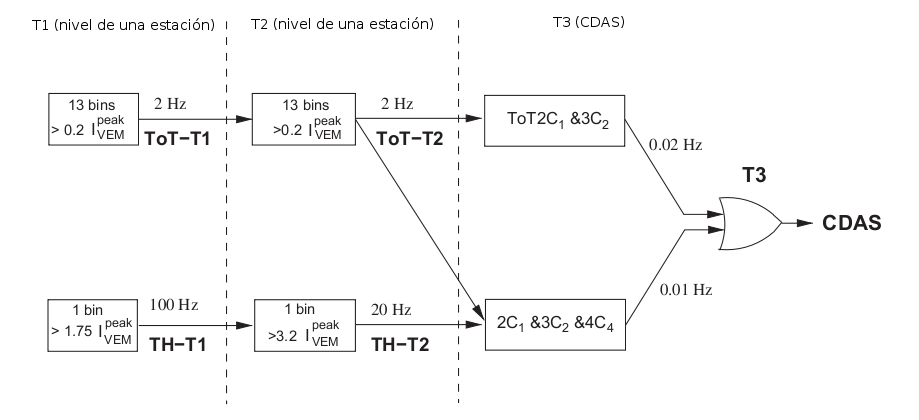
\includegraphics[width=0.9\textwidth]{fig/detectorAuger/Trigger_2}
				\caption{\label{fig:diagtrig} Jerarqu\'ia de trigger hasta T3.}
				\end{center}
			\end{figure}
			
			\titulo{Trigger f\'isico T4} Este nivel de trigger se aplica para remover lso eventos que dieron T3 debido a disparos casuales de los tanques.
			Con este fin, se clasifican los eventos en dos nuevas categor\'ias:
			
			\begin{itemize}
			\item 3-ToT: Para cumplir con esta categor\'ia se deben encontrar tres tanques T2-ToT en la primer corona de alguno de los tres y formando un tri\'angulo. Los tanques deben estar alejados como m\'aximo \cant{2700}{m}. Tambi\'en se pide que el tiempo de disparos de las estaciones entre si sea compatible con un frente que se mueve a la velocidad de la luz. Esta categor\'ia es muy eficiente filtrando eventos casuales, m\'as aun si la direcci\'on de arribo de la lluvia es $<60º$ (\cant{98}{\%} de eficiencia en estas condiciones). Los eventos accidentales que pasan esta categor\'ia son menos que uno por d\'ia.
			\item $\rm 4C_1$: Este criterio requiere cuatro estaciones dentro de la primer corona de alguno de los tanques, todas con cualquier T2. Tambi\'en se pide que los tiempos de arribo sean compatibles con un frente que se mueve a la velocidad de la luz. La frecuencia con la que se da este trigger es \cant{\approx 0.001}{Hz} y la eficiencia para lluvias de $<60º$ es \cant{\approx 100}{\%}.
			\end{itemize}
			\vspace{0.5cm}
			
			\titulo{Trigger de calidad T5} Esta categor\'ia se define para filtrar lluvias incompletas debido a que fueron detectadas en el borde del detector o en alg\'un agujero debido a estaciones fuera de servicio al momento de arribo.
			De esta manera se busca evitar errores al momento de la reconstrucci\'on debido a que tal vez la parte m\'as importante de la lluvia no fue detectada.
			Se definen las dos siguientes categor\'ias:
			
			\begin{itemize}
			\item 6T5: Esta categor\'ia requiere que la estaci\'on con mayor se\~nal integrada se encuentre rodeada de seis estaciones activas.
			\item ICRC T5 o 5T5: Igual que 6T5, pero este requiere s\'olo 5 de las 6 estaciones y que el n\'ucleo reconstruido de la lluvia se encuentre dentro de un tri\'angulo formado por tres estaciones activas.
			\end{itemize}
			
			En la figura \ref{fig:diagtrig2} se muestra la jerarqu\'ia de triggers desde T3.
			
			\begin{figure}[h!]
				\begin{center}
				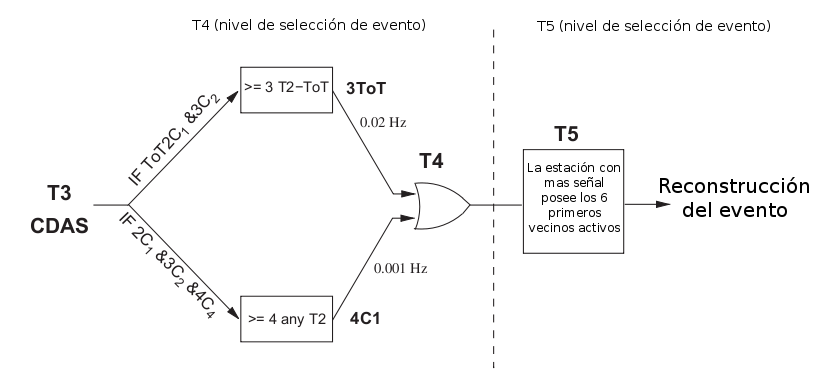
\includegraphics[width=0.9\textwidth]{fig/detectorAuger/Trigger_3}
				\caption{\label{fig:diagtrig2} Jerarqu\'ia de trigger desde T3.}
				\end{center}
			\end{figure}

\chapter{Lluvias atmosf\'ericas extendidas}
\label{ch:easAuger}

\section{Generalidades}

A fines de la década del treinta Pierre Auger observó que la coincidencia de disparo entre detectores de CR separados varios kilómetros era mayor a la esperada para eventos independientes. Explicó éste hecho postulando la existencia de partículas muy energéticas que, al interactuar  en la alta atmósfera, pudieran generar nuevas partículas de alta energía capaces, a su vez, de repetir el proceso. De esta manera se inicia una reacción de multiplicación en cadena que lleva hoy el nombre de lluvia atmosférica extendida (EAS, por su sigla en inglés). 

Tras 70 años de investigación, la estructura y evolución de las cascadas atmosféricas se considera bien comprendida.
Tras la primera interacción, su desarrollo puede describirse como un núcleo de partículas de alta energía (usualmente hadrones), que avanza a lo largo del eje de la lluvia produciendo electrones, muones y fotones menos energéticos, pero con mayor momento transverso relativo, que difunden en la dirección radial (ver figura ~\ref{fig:lluvia1}). Así, las cascadas están formadas por tres componentes: hadrónica, muónica y electromagnética (ver figura \ref{fig:showerSchema}).

La estructura detallada es complicada y depende de gran cantidad de factores como partícula primaria, su energ\'ia o profundidad de la interacción entre otras.

%
\begin{figure}[ht]
\begin{center}
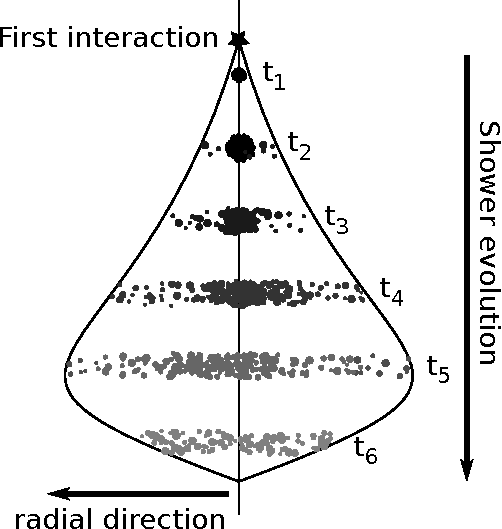
\includegraphics[width=0.75\textwidth]{fig/EASAuger/lluvia1_english.pdf}
\caption{Esquema de la evolución de una cascada atmosférica. Tras la primera interacción se forma un núcleo de partículas de alta energía (usualmente hadrones), que avanza a lo largo del eje de la lluvia produciendo nuevas partículas menos energéticas, pero con mayor momento transverso relativo, que difunden en la dirección radial}
\label{fig:lluvia1}
\end{center}
\end{figure}
%
%
\begin{figure}[ht]
\begin{center}
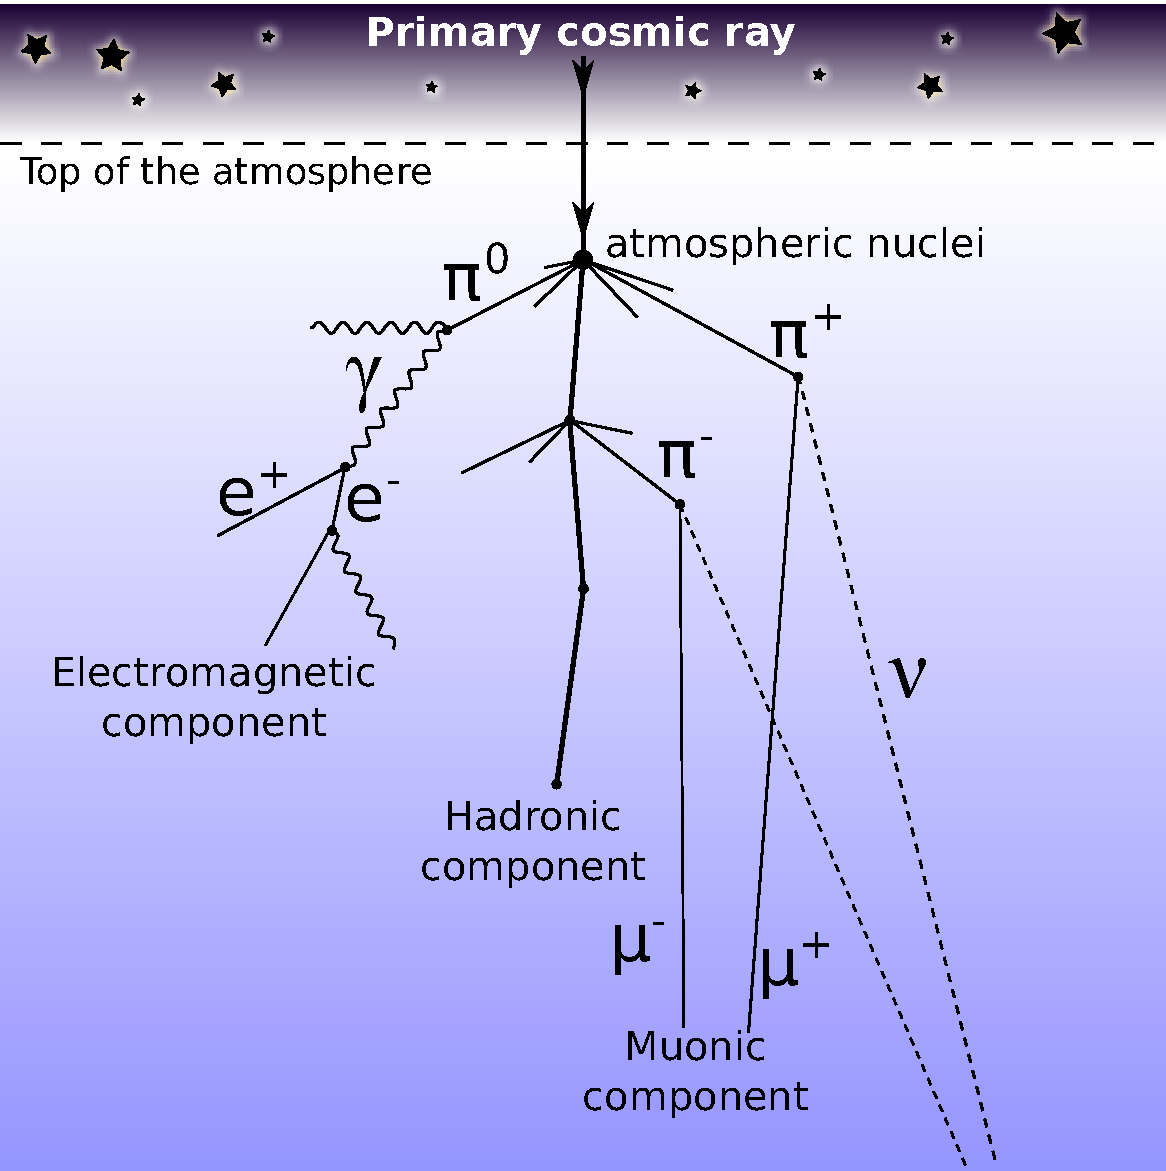
\includegraphics[width=0.75\textwidth]{fig/EASAuger/showerSchema_english.pdf}
\caption{Diagrama esquemático de la estructura de una cascada atmosférica.}
\label{fig:showerSchema}
\end{center}
\end{figure}
%

En la actualidad se considera que la gran mayoría de las cascadas con energía superior a $10^{16}$~eV son iniciadas por UHECR hadrónicos \cite{CONSEGUIR}. 
En estas lluvias, el número de hadrones aumenta rápidamente durante las primeras etapas de la cascada, predominando la generaci\'on equiprobable de $\pi^{0}$, $\pi^{+}$ y $\pi^{-}$.
Dado de que el decaimiento de los $\pi^{0}$ es el $(98.823\pm0.034)\%$ \cite{Agashe:2014kda} de las veces a $\gamma\gamma$ y el $(1.174\pm0.035)\%$ a $e^+e^-\gamma$, en cada generación alrededor del 30\% de la energía de la componente hadr\'onica es transferida a la componente electromagnética mediante este proceso.

Por otro lado, la energ\'ia es entregada a la componente muónica de la lluvia crece más lentamente. 
Si bien los muones son producidos principalmete a partir del decaimiento de piones cargados, que decaen el $(99.98770\pm0.00004)\%$ a $\mu^{\pm}\nu_\mu$~\cite{Agashe:2014kda}, debido a la dilatación temporal, los $\pi^{\pm}$ más energéticos tienen menor probabilidad de decaer antes de interactuar y asi tranferir parte de su energía a la componente electromagnética.

Por todo esto, en las etapas finales de la cascada alrededor del 90\% de la energía de la partícula primaria es disipada por la componente electromagnética mediante ionización.
La restante es transportada por muones y neutrinos provenientes de $\pi^{\pm}$ que hayan decaído antes de interactuar.

\section{Lluvias iniciadas por hadrones}
En esta sección se comentará un modelo simplificado de lluvia desarrollado originalmente por Heitler \cite{hei54} a mediados de los años 50. Si bien el modelo es demasiado simple para obtener resultados cuantitativos precisos, ayuda a comprender cualitativamente la dinámica de las lluvias.

\subsection{Componente electromagnética - Modelo de Heitler}
En el cálculo de la evolución de la porción electromagnética de la lluvia se considera que cada electrón radía (bremsstrahlung) un único fotón después de viajar una distancia $d=\lambda \ln 2$, donde $\lambda\simeq38$~g~cm$^{-2}$ es la longitud de radiación propia del medio\footnote{$d$ es la distancia promedio para la cual un electrón habrá irradiado la mitad de su energía}. Simultáneamente se propone que cada fotón producirá un par $e^{-}$ $e^{+}$ después de recorrer esta misma distancia.
Este proceso se esquematiza en la figura \ref{fig:heilter}.
%
\begin{figure}[ht]
\begin{center}
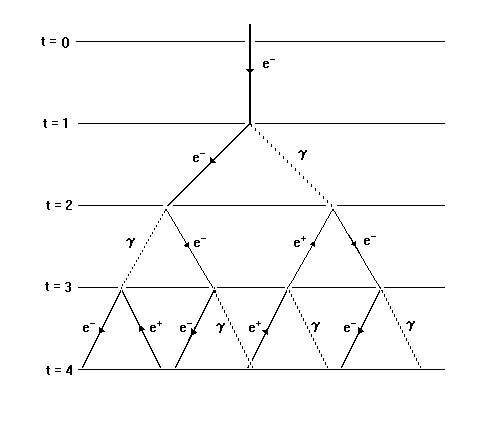
\includegraphics[width=0.75\textwidth]{fig/EASAuger/heilterSchema}
\caption{Esquema del modelo de Heilter. Luego de cada longitud de radiación ($t=nd/\lambda$) los $e^\pm$ emiten un fotón, mientras que los fotones producen un par $e^+e^-$.}
\label{fig:heilter}
\end{center}
\end{figure}
%
En ambos casos se toma que la energía se reparte equitativamente entre las partículas hijas. Después de $n$ pasos la lluvia contará con $2^{n}$ partículas entre electrones, positrones y fotones. El modelo considera que la generación de nuevas partículas se detiene cuando la energía perdida por colisiones\footnote{ionizacion y excitaci\'on de las mol\'eculas del aire, esencialmente $N_2$ y $O_2$} es mayor que la necesaria para los procesos de bremsstrahlung y producción de pares. En el aire esta energía de corte es de aproximadamente \cant{85}{MeV}. En este punto la cantidad de partículas es máxima y valen las siguientes ecuaciones:
%
\begin{equation}
\label{hi1}
E_p = E_{corte} N_{max} = E_{corte} 2^{n_{max}}
\end{equation}
%
\begin{equation}
\label{hi2}
X_{max}=n_{max} d
\end{equation}
%
con $X_{max}$ la coordenada donde la lluvia alcanza la máxima cantidad de partículas $N_{max}$ luego de $n_{max}$ pasos y $E_p$ la energía del primario.
Despejando $n_{max}$ de (\ref{hi1}) y reemplazando en (\ref{hi2}) se obtiene para Xmax
%
\begin{equation}
\label{hi3}
X_{max} = n_{max} \lambda \ln2=\lambda \ln\left(\frac{E_{0}}{E_{corte}}\right)
\end{equation}
%
Las relaciones \ref{hi1} y \ref{hi3}, que pueden resumirse en \ref{hi4}, se recuperan mediante simulaciones a partir de primeros principios.
%
\begin{equation}
\label{hi4}
X_{max} \sim \ln E_{p}
\hspace*{15mm}
N_{max} \sim E_p
\end{equation}
%

\subsection{Componente hadrónica y muónica}
Para modelar la componente hadrónica de la lluvia se utiliza un esquema muy similar al utilizado para la electromagnética.
Se considera que la totalidad de los hadrones son piones ($\pi^{\pm}$ y $\pi^{0}$). Los $\pi^{\pm}$ al interactuar con n\'ucleos de la atm\'osfera generan $N \pi^{\pm}$ y $\frac{1}{2}N \pi^{0}$ después de atravesar una feta de atmósfera de ancho $d=\lambda \ln2$ siendo $\lambda$ la longitud de interacción para partículas que interactúan fuertemente.
Los $\pi^{0}$ decaen inmediatamente en dos fotones que pasan a formar parte de la componente electromagnética y los $\pi^{\pm}$ continúan la cascada hadrónica hasta que su energía no les permite generar nuevos piones.
En este punto los $\pi^{\pm}$ s\'olo pueden decaer a muones.
Estos muones, provenientes de $\pi^{\pm}$ de baja energía, forman la totalidad de la componente muónica de la lluvia.
El alto poder de penetración de los muones les permite atravesar la atmósfera sin interactuar en el camino, por lo que generalmente alcanzan la superficie de la Tierra antes que la componente electromagnética.

\subsection{Lluvias inclinadas}
\label{sbsc:inclinadas}
%
El término ``lluvias inclinadas'' se refiere a lluvias cuyo ángulo zenital $\theta$ es mayor a $60^{\circ}$.
Con el fin de motivar esta definición es interesante estudiar la cantidad de materia que la lluvia tiene que atravezar hasta alcanzar la Tierra como función de $\theta$.
En la figura \ref{fig:slant_depth} se muestra como entre $0^{\circ}$ y $60^{\circ}$ el cambio en la profundidad es un factor $\sim 2$ respecto de su contraparte vertical, \cant{\sim1000}{g/cm^{2}}.
A partir de este punto la profundidad crece rápidamente, alcanzando un factor $\sim 36$ a $\theta=90^{\circ}$.
%
\begin{figure}[h!]
\begin{center}
$
\begin{array}{cc}
 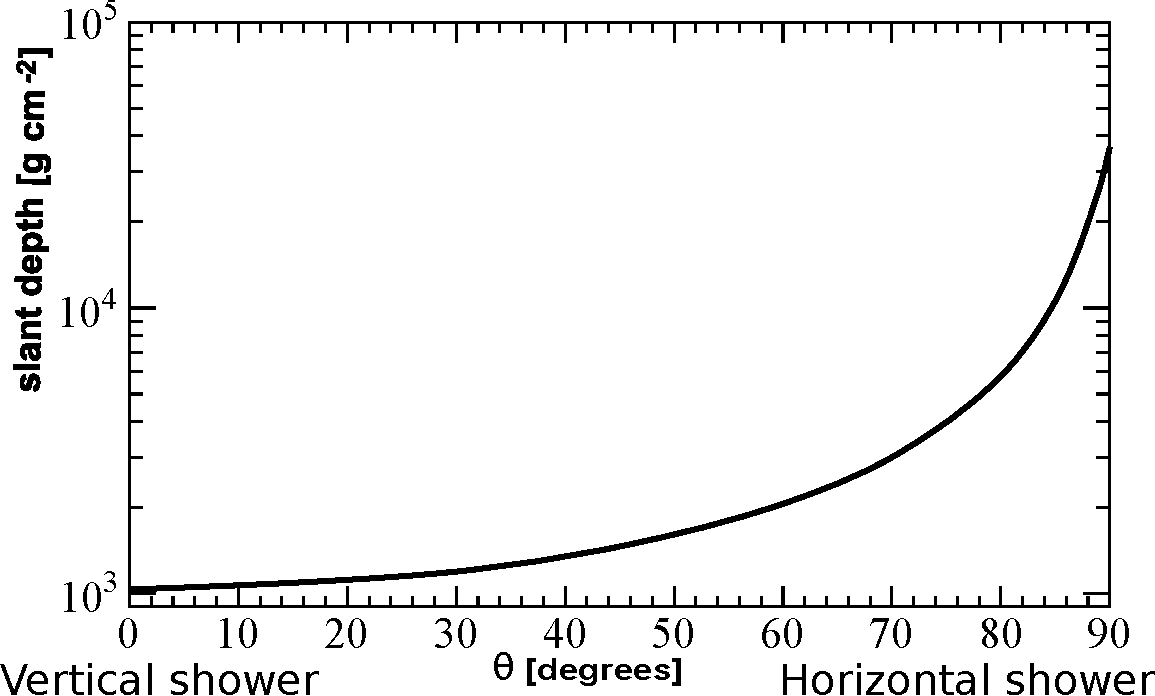
\includegraphics[width=0.47\textwidth]{fig/EASAuger/slant_depth_english.pdf} & 
 \raisebox{0.8\height}{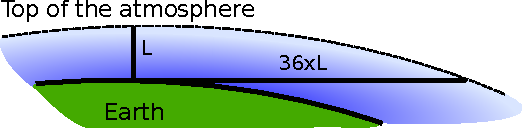
\includegraphics[width=0.47\textwidth]{fig/EASAuger/slantCartoon_english.pdf}}
\end{array}
$
\caption{\textit{Izquierda:} Profundidad atmosférica como función del ángulo zenital $\theta$.
La cantidad de materia crece rápidamente si $\theta>60^{\circ}$.
\textit{Derecha:} Una lluvia completamente horizontal atravieza 36 veces más materia que una vertical.
}
\label{fig:slant_depth}
\end{center}
\end{figure}
%

La mayor parte los rayos cósmicos con energías superiores a \cant{10^{16}}{eV} son protones o n\'ucleos.
Dado que su longitud de interacción en la atmósfera es \cant{\sim50}{g/cm^{2}}, es correcto considerar que estas interact\'uan en el tope de la atmósfera.
En consecuencia, para lluvias con $\theta>70^\circ$, tanto la componente hadrónica como la electromagnética son completamente absorbidas por la atmósfera\footnote{como puede deducirse de la figura \ref{fig:effDG_tr_id} del cap\'itulo \ref{ch:resAuger} de esta tesis, luego de \cant{2000}{g/cm^2} la componente electromagn\'etica es absorbida por la atm\'osfera.}, por lo que sólo la componente muónica alcanza el suelo, como se esquematiza en la figura \ref{fig:horizontalHad}.
Como resultado, a nivel del suelo las lluvias horizontales son fundamentalmente diferentes de las verticales.
%
\begin{figure}[h!]
\begin{center}
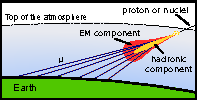
\includegraphics[width=0.7\textwidth]{fig/EASAuger/horizontal2_english.pdf}
\caption{Las lluvias inclinadas producidas por protones o n\'ucleos se inician cerca del tope de la atmósfera.
Las componentes hadrónica y electromagnética se absorben rápidamente, por lo que sólo los muones alcanzan el suelo.
}
\label{fig:horizontalHad}
\end{center}
\end{figure}

\section{Lluvias atmosf\'ericas iniciadas por neutrinos}
\label{sc:easNu}

Existen dos mecanismos principales mediante los cuales los neutrinos pueden iniciar lluvias atmosféricas que puedan producir señales en detectores de superficie:
\begin{itemize}
 \item Lluvias descendentes (DG, down going)
 %Un neutrino deposita algo de su energía en la atmósfera generando una lluvia descendente cuyas partículas alcanzan el suelo.
 \item Lluvias rasantes iniciadas por neutrinos tau (ES, earth-skimming)
 %Un neutrino ascendente interactúa con la corteza de la tierra y alguno de sus productos de decaimiento genera una cascada en la atmósfera muy cerca del suelo.
\end{itemize}

\subsection{Lluvias descendentes}
\label{sbsc:easDG}

De acuerdo con el modelo estandar (SM por sus siglas en inglés), los neutrinos interactúan mediante la gravedad y la fuerza débil, pero sólo esta última puede ser utilizada para detectar neutrinos individuales.
Su principal mecanismo de interacción en la atmósfera es la dispersión inelástica profunda (DIS por sus siglas en inglés, \emph{Deep Inelastic Scattering}) con un n\'ucleo de la misma. Los posibles canales se esquematizan en la figura \ref{fig:SM_nu_int} para los diferentes sabores de neutrinos.
En todos los casos, cerca del \cant{20}{\%} de la energía del neutrino primario se transfiere al jet hadrónico mediante los fragmentos del núcleo resultantes de la interacción.
El resultado de este proceso es una cascada de características similares a las iniciadas por protones o núcleos.

El \cant{80}{\%} restante de la energía se transfiere a un leptón ultra energético que según el caso puede contribuir o no a la EAS generada.
%
\begin{figure}[ht]
\begin{center}
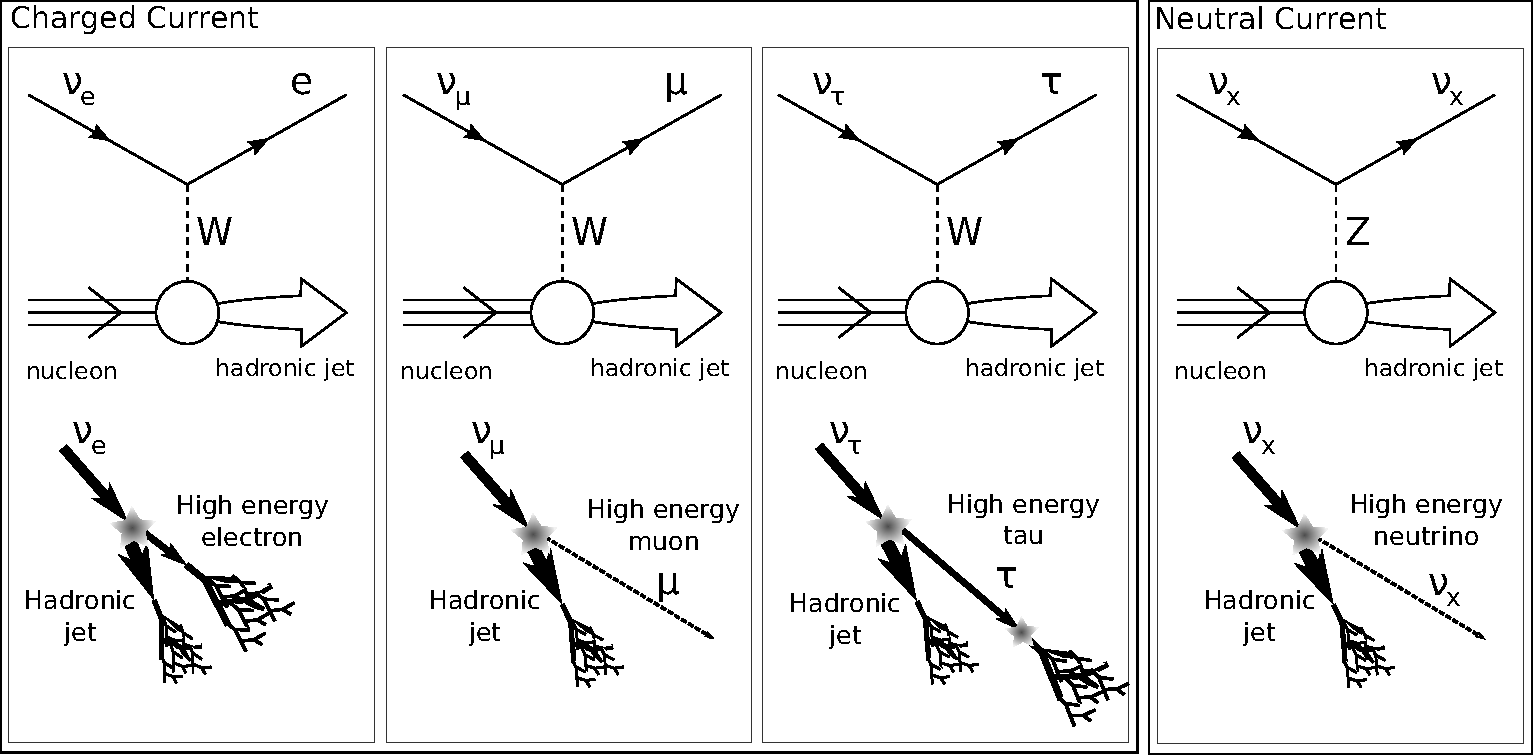
\includegraphics[width=1.0\textwidth]{fig/EASAuger/nu_channels_english.pdf}
\caption{Canales de interacción para neutrinos de acuerdo con el Modelo Estandar.
En todos los casos se muestra el diagrama de Feynman al orden más bajo.
Para todos los canales, el jet resultante de la fragmentación del núcleo inicia una lluvia hadrónica que posee alrededor del \cant{20}{\%} de la energía del neutrino incidente.
El electrón producido en la interacción via corriente cargada (CC) genera una cascada electromagnética que se suma al jet hadrónico.
Cuando el neutrino primario es un $\nu_{\tau}$ que interact\'ua via CC el $\tau$ generado puede viajar una distancia considerable antes de decaer y generar una cascada, a veces muy cercana al suelo.
Estas se denominan \emph{cascadas double bang}.
Finalmente, en el caso de tener un $\nu_{\mu}$ primario, el $\mu$ resultante en la mayor parte de los casos no genera lluvia alguna.
}
\label{fig:SM_nu_int}
\end{center}
\end{figure}

En el caso de interacción via corriente neutra (NC), luego de perder energía el neutrino escapa sin generar cascada alguna, quedando la cascada con sólo el \cant{20}{\%} de la energía del primario.

Si la lluvia es iniciada por un $\nu_e$ via corriente cargada (CC), el electrón resultante inicia una cascada electromagnética que se superpone con la hadrónica producida por los fragmentos del núcleo.
En este caso, toda la energía del neutrino primario es transferida a la lluvia.

Aunque el mecanismo fundamental mediante el que se inician, las lluvias generadas por $\nu_{\mu}$ via CC son muy similares a las generadas via NC ya que las probabilidades de que el $\mu$ resultante de la interacción decaiga o interactúe antes de llegar al suelo son pequeñas\footnote{La probabilidad de que un $\mu$ de \cant{10^{18}}{eV} decaiga antes de llegar al suelo es de $\sim10^{-6}$ mientras que la probabilidad de que sufra DIS o bremsstrahlung es del orden de $10^{-3}$ \cite{cite:tesisJavier}} 

En el caso de un $\nu_{\tau}$ que interactúa via CC al proceso se le agrega una particularidad.
Al igual que el $\mu$, el $\tau$ resultante es una partícula muy penetrante pero en este caso su vida media es siete \'ordenes de magnitud menor.
Debido a \'esto, luego de viajar una distancia apreciable\footnote{\cant{5}{km} para un $\tau$ de \cant{10^{17}}{eV}} y, como se discutir\'a en el cap\'itulo \ref{ch:simulacionAuger}, decaerá generando en el \cant{\sim80}{\%} de los casos una cascada detectable, que a su vez será el \cant{\sim25}{\%} de caracter electromagnético y el \cant{\sim75}{\%} restante hadrónico.
Este tipo de cascadas, muy características, se conocen como ``Double--Bang'' (DB).
%
\begin{figure}[h!]
\begin{center}
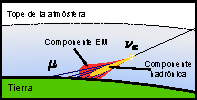
\includegraphics[width=0.7\textwidth]{fig/EASAuger/horizontal_deep_english.pdf}
\caption{Los neutrinos pueden iniciar lluvias inclinadas profundas en la atmósfera.
En este tipo de lluvias tanto la componente electromagnética como la muónica pueden llegar al suelo.
Comparar con la figura \ref{fig:horizontalHad}.
}
\label{fig:horizontalNu}
\end{center}
\end{figure}

El camino libre medio para neutrinos de \cant{10^{18}}{eV} es de \cant{\sim10^8}{g/cm^{2}}\cite{cite:Gandhi}. 
Dado que este valor es mucho mayor que el espesor m\'asico de la atmósfera, incluso para $\theta\sim90^\circ$, los neutrinos pueden interactuar básicamente en cualquier punto de la atmósfera con la misma probabilidad.
En particular, tinen la capacidad de iniciar lluvias lo suficientemente profundas como para que tanto la componente electromagnética como la muónica alcancen el suelo (ver figura \ref{fig:horizontalNu}).
Por otro lado, esto es pr\'acticamente imposible para lluvias iniciadas por hadrones o núcleos, ya que interactúan usualmente en el primer centenar de gramos.
Por esto mismo, la estrategia utilizada para observar neutrinos con detectores de superficie se basa en la detección lluvias inclinadas en las que la componente electromagnética no haya sido absorbida por la atmósfera. Este canal de detección es llamado Down-going (DG).

%
\subsection{Lluvias rasantes iniciadas por neutrinos tau}
\label{sc:EStauInducedShowers}
%
Otro tipo de lluvias muy interesante son las que pueden ser iniciadas por neutrinos que interactúan en la corteza terrestre.
En este caso, tanto el jet hadrónico producido en la interacción con el núcleo como el electrón producido en el caso de un $\nu_e$ incidente son rápidamente absorbidos por la materia, sin embargo, los leptones $\mu$ y $\tau$ producidos al incidir un $\nu_{\mu}$ o un $\nu_{\tau}$ pueden escapar de la Tierra debido a que son muy penetrantes.
Una vez más, debido a su vida media larga, los $\mu$ que escapen de la Tierra iniciarán usualmente una luvia muy alto en la atmósfera, por lo que las partículas secundarias rara vez alcanzarán el suelo.
Por otro lado, los leptones $\tau$ tienen baja sección eficaz, lo que les permite escapar de la Tierra hacia la atmósfera, pero a su vez poseen un tiempo de vida media que les permite decaer lo suficientemente cerca de la superficie\footnote{La longitud de decaimiento es $\lambda_{d}=c\tau_{\tau}\gamma_{\tau}=49\text{km}\frac{E_{\tau}}{\text{EeV}}$}, iniciando una cascada cuyas partículas secundarias pueden alcanzar el suelo. Este canal de detección es llamado Earth-Skimming (ES) y se esquematiza en la figura \ref{fig:esNu}.

\begin{figure}[ht]
\begin{center}
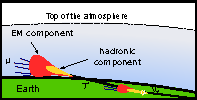
\includegraphics[width=0.7\textwidth]{fig/EASAuger/horizontal_es_english.pdf}
\caption{Un $\nu_{\tau}$ puede interactuar en la Tierra via CC dando como resultado un $\tau$ que puede emerger a la atmósfera e iniciar una EAS muy cerca de la superficie.
Aunque \'esta es ascendente, si el $\tau$ emergente posee un ángulo zenital entre $90^\circ$ y $95^\circ$ las partículas que llegan al suelo suelen ser suficientes para detectar la lluvia.}
\label{fig:esNu}
\end{center}
\end{figure}

Dado que la densidad de la corteza terrestre es $\sim1000$ veces mayor a la del aire, funciona como un blanco muchísimo mas masivo que la atmósfera para los neutrinos.
Como ejemplo, el camino libre medio para un neutrino de \cant{10^{18}}{eV} en la Tierra\footnote{la densidad de la Tierra es \cant{\rho\sim2.65}{\frac{g}{cm^3}}} es de \cant{\sim620}{km}.
Por otro lado, bajo la aproximación de Tierra esférica, la distancia que debe recorrer un neutrino para atravezarla es $d\sim2R\cos{\theta}$, donde $R$ es el radio de la Tierra. 
En consecuencia, como para $91^{\circ}$ se obtiene \cant{d\sim220}{km}, se concluye que \cant{\sim30}{\%} de los neutrinos interactuarán en esas condiciones.
Luego, es necesario considerar la probabilidad de que el $\tau$ escape de la Tierra sin perder demasiada energía y a su vez decaiga lo suficientemente cerca del suelo, pero esto se analizará en detalle en la sección \ref{sc:earthInteraction}.

%\chapter{Estrategia de la búsqueda}
\label{ch:estrategiaAuger}

En este capítulo se presenta la estrategia utilizada en la búsqueda de neutrinos ultra-energéticos con el Observatorio Pierre Auger.

Como se mostró en la sección \ref{sbsc:inclinadas}, el desafío a la hora de detectar UHE$\nu$'s utilizando un detector de superficie es lograr identificar los eventos que estos diparan del inmensamente más poblado fondo de lluvias hadrónicas.
Esto puede lograrse separando las lluvias jóvenes dentro de los eventos inclinados.

En la figura \ref{fig:augerNu} se resumen los posibles canales de detección de neutrinos con el observatorio Pierre Auger, que ya fueron detallados en la sección \ref{sc:easNu}.
	\begin{figure}[ht!]
		\centering
		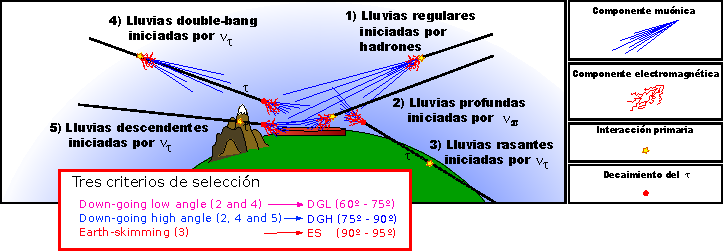
\includegraphics[width=\textwidth]{./fig/estrategiaAuger/auger_nu}
		% curveEarthSketch.png: 2404x1199 pixel, 150dpi, 40.70x20.30 cm, bb=0 0 1154 575
		\caption{\label{fig:augerNu}
		Posibles canales de detección de neutrinos en auger. Se detallan los tres análisis que fueron optimizados para identificar neutrinos provenientes de los diferentes canales.
		}
	\end{figure}
Debido a la diferencias esenciales que presentan estos canales de detección, en Auger existen actualmente tres búsquedas optimizadas para distintos rangos de ángulo zenital:
\begin{itemize}
 \item DGL: optimizado para buscar neutrinos down-going con ángulo entre $60^\circ$ y $75^\circ$.
 \item DGH: idem DGL pero para ángulos entre $75^\circ$ y $90^\circ$. 
 \item ES: optimizado para detectar neutrinos earth-skimming para ángulos entre $90^\circ$ y $95^\circ$.
\end{itemize}

En los tres casos, la estrategia utilizada para la búsqueda fue del tipo \emph{análisis ciego}, cuyo proceder se esquematizan en la figura \ref{fig:strAuger}.
	\begin{figure}[ht!]
		\centering
		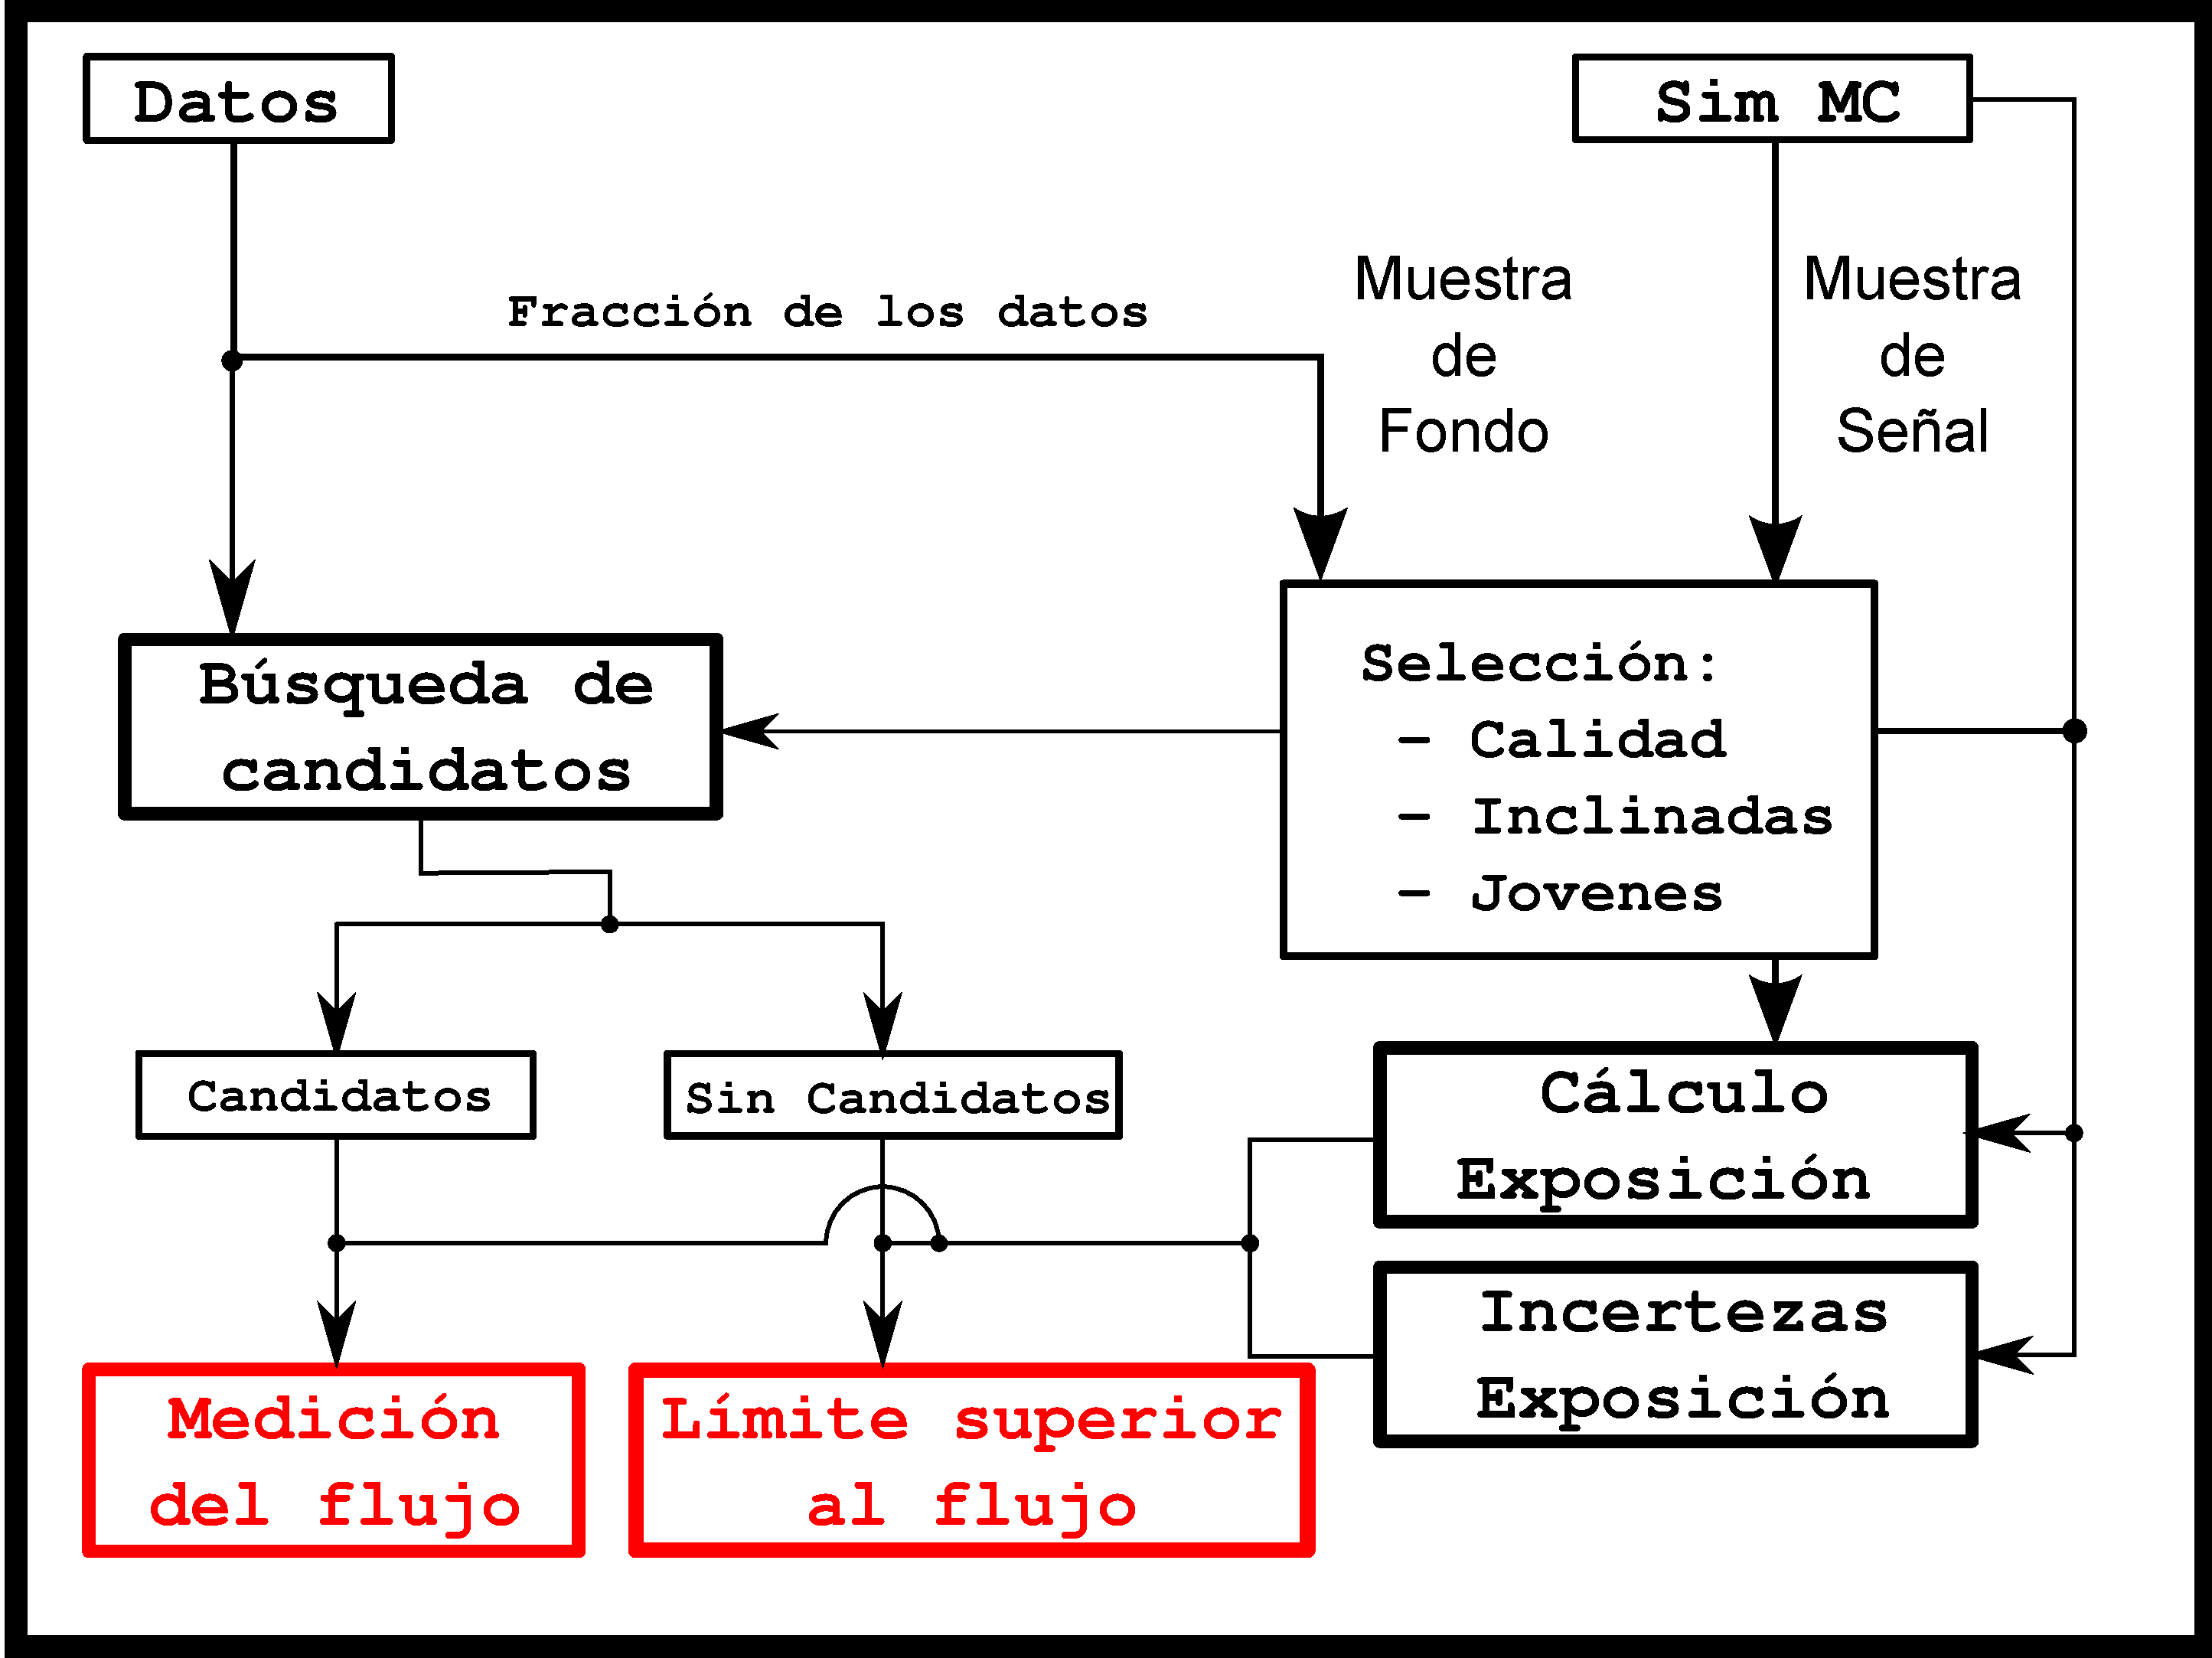
\includegraphics[width=\textwidth]{./fig/estrategiaAuger/analysisSchema}
		\caption{\label{fig:strAuger}
		Esquema de la estrategia utilizada en las búsquedas de neutrinos con el Observatorio Pierre Auger.
		}
	\end{figure}
Este consiste en definir un criterio de selección mediante el cual se decidirá si un evento es candidato a neutrino o no, sin utilizar datos o utilizando una pequeña fracción de los mismos que luego no podrá ser utilizada para la búsqueda.

Para definir este criterio es necesario contar con una muestra de señal y otra de fondo.
En los tres análisis se utilizaron simulaciones de Monte Carlo para generar una muestra de señal y una pequeña fracción de los datos ($\sim15\%$) como muestra de fondo, debido a que se encuentran completamente dominados por eventos que no son neutrinos.
Una vez definidas las muestras de señal y fondo, se eligieron criterios de calidad con el fin de eliminar eventos espureos y se optimizaron cortes en diferentes variables del detector que permiten elegir las lluvias jóvenes entre las inclinadas.
Así, con el criterio de selección listo es posible, por un lado calcular la exposición del detector a los distintos tipos de neutrinos y estimar las incertezas sistemáticas cometidas, y por el otro realizar la búsqueda de candidatos sobre los datos que no fueron utilizados hasta el momento.
Luego, si hubiese candidatos sería posible informar la magnitud de el flujo con su error, o en caso contrario ponerle una cota superior.

En los próximos capítulos se abordarán las distintas etapas de este análisis para las tres búsquedas.

% \textbf{DEBERIA MENCIONAR LAS TRES TESIS EN ESTA SECCION ME PARECE}

\chapter{Obtención de la muestra de señal: Cadena de simulaciones}
\label{ch:simulacionAuger}

Dada la complejidad del problema, la \'unica manera viable de obtener una muestra de señal en el detector es mediante simulaciones.
Para ello, son necesarios una serie de programas que se encargan de simular las distintas etapas del proceso de detecci\'on:
\begin{description}
 \item[Interacción primaria:] esta incluye el procesamiento de la interacción neutrino nucleón y cuando corresponda el del decaimiento del \tauon{}. Para esto se utilizan respectivamente dos programas específicos llamados \herwig{} y \tauola{}.
 \item[Desarrollo de la EAS:] una vez obtenido los productos de la primera interacción se utiliza un programa llamado \aires{}, que simula la evolución de la cascada a través de la atmósfera.
 \item[Señal en el detector:] con la lista de partículas que llegan al suelo es posible simular la señal que estas generarían en el detector, utilizando el software oficial de la colaboración llamado \Offline{}.
\end{description}

	\section{Interacción primaria: \herwig{} - \tauola{}}
	
	\aires{} no incluye herramientas para para procesar la interacción neutrino-nucleón ni el decaimiento \tauon{}'s.
	Para salvar este inconveniente, fue necesario utilizar programas complementarios que devuelvan una lista de partículas y sus cuadrimomentos que luego puedan ser utilizadas para iniciar la EAS.
	
	\subsection{Interacción neutrino-nucleón: \herwig{}}
	
	La interacción neutrino-nucleón fue procesada utilizando el paquete \herwig{}~\cite{cite:herwig}.
	\herwig{} es un generador de eventos de alta energía capaz de realizar una simulación detallada de los procesos QCD, incluidas las lluvias partónicas generadas y su hadronización posterior.
	Para ello se tomaron en cuenta las interacciones via CN  y la de todos los sabores via CC.

	La fracción de energía transferida por el neutrino primario a la lluvia depende en gran medida del canal de interacción débil involucrado.
	Si la lluvia es iniciada por un $\nu_e$ vía el canal de CC, el 100\% de la energía del neutrino primario es transferida.
	En contraposición, en las interacciones CN, se produce un neutrino secundario en lugar de un electrón. Este neutrino lleva, en promedio, el 80\% de la energía del primario.
	Como la probabilidad de que este neutrino secundario escape sin interactuar es muy alta, solo una fracción de la energía del primario es transferida a la cascada. 

	A las energías involucradas, las lluvias iniciadas por $\nu_e$, $\nu_{\mu}$ y $\nu_{\tau}$ vía CN son indistinguibles desde el punto de vista del jet hadrónico producido.
	Es por ello que simular uno solo de los tres sabores es suficiente para describir los tres canales de CN.

	Las lluvias iniciadas por $\nu_{\mu}$ vía CC son muy similares a las de NC pese a que la interacción fundamental involucrada es diferente.
	Tal como se discute en la sección \ref{sc:easNu}, es muy poco probable que el muón de alta energía producido decaiga o interactúe antes de alcanzar la tierra.
	De esta manera, es indistinguible de un neutrino secundario que emerge de una interacción de CN. 
	Además, debido a que la distribución de la fracción de enegía que se transmite al jet (inelasticidad) es muy similar en interacciones vía CN y CC  (ver Fig.~\ref{fig:inelast}), el conjunto de simulaciones producido para los canales de CN puede se utilizado para describir, con excelente aproximación, el canal $\nu_{\mu}$ vía CC.
	%
	\begin{figure}[ht]
	\begin{center}
	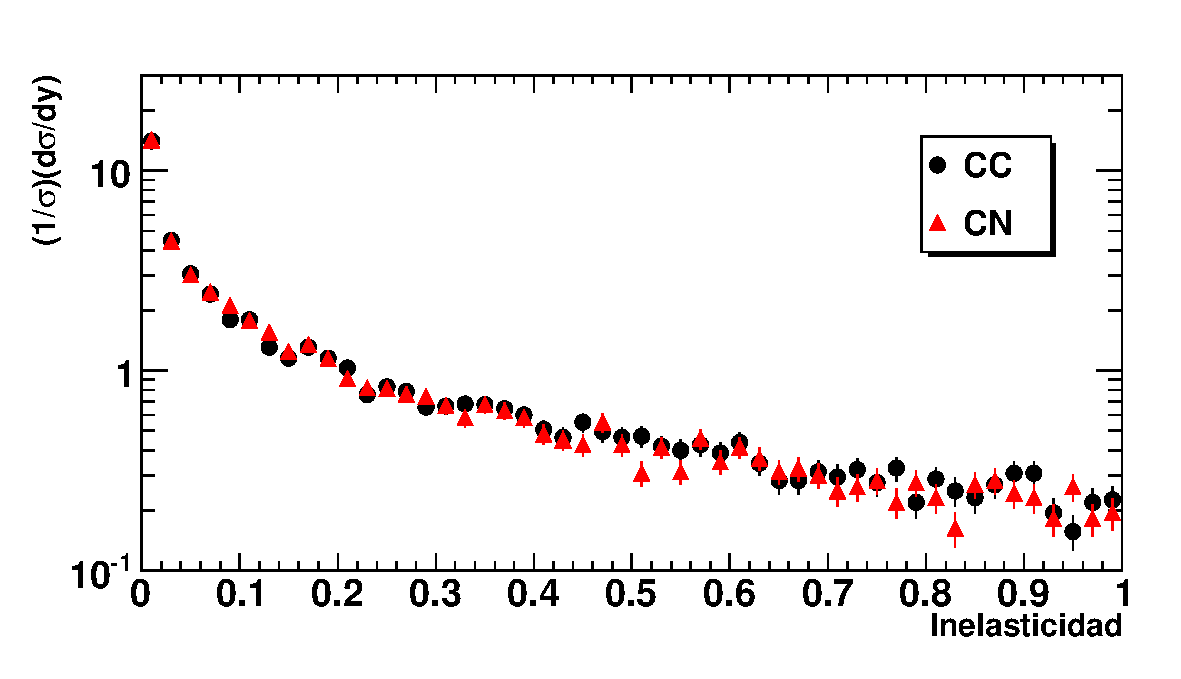
\includegraphics[width=0.80\textwidth]{fig/simulacionAuger/Inelasticity}
	\caption{Comparación de la distribución de inelasticidad para interacciones $\nu$--nucleón de alta energía para CN y CC.}
	\label{fig:inelast}
	\end{center}
	\end{figure}
	%

	
	\subsection{Decaimiento del \tauon{}: \tauola{}}
	
	El canal $\nu_{\tau}$ vía CC es un caso que requiere un tratamiento más sofisticado tanto para eventos DG o ES.
	En ambos casos, luego de propagarse a trav\'es de la atm\'osfera, el \tauon{} decae generando una gran variedad de part\'iculas secundarias que luego inician la EAS.
	Para generar eventos utilizando la probabilidad de decaimiento a cada canal pueden utilizarse un conjunto de librer\'ias llamadas \tauola{}.
	Estas consisten en varios programas Monte Carlo que implementan decaimientos lept\'onicos y semilept\'onicos.
	Como salida se entrega la topolog\'ia completa del evento, incluyendo neutrinos, resonancias intermedias y la estructura completa de spin durante el desarrollo del decaimiento.
	
	La tabla \ref{tab:tauDecay} muestra los primeros ocho canales de decaimiento del \tauon{} utilizados por \tauola{}, que representa el $\sim96\%$ de los eventos esperados.
	\begin{table}[h]
		\begin{center}
		\begin{tabular}{|c|l|l|}
		% \hline
		\hline
		\# &Canal   & Probabilidad (\%) \\
		\hline
		1&$\tau^{-}\rightarrow \pi^{-}\pi^{0}\nu_{\tau}$   & $\sim$25.5 \\
		2&$\tau^{-}\rightarrow e^{-}\bar{\nu_{e}}\nu_{\tau}$   & $\sim$17.9 \\
		3&$\tau^{-}\rightarrow \mu^{-}\bar{\nu_{\mu}}\nu_{\tau}$   & $\sim$17.4 {\bf No genera EAS}\\
		4&$\tau^{-}\rightarrow \pi^{-}\nu_{\tau}$   & $\sim$10.9 \\
		5&$\tau^{-}\rightarrow 2\pi^{-}\pi^{+}\nu_{\tau}$   & $\sim$9.3 \\
		6&$\tau^{-}\rightarrow \pi^{-}2\pi^{0}\nu_{\tau}$   & $\sim$9.3 \\
		7&$\tau^{-}\rightarrow 2\pi^{-}\pi^{+}\pi^{0}\nu_{\tau}$   & $\sim$4.6 \\
		8&$\tau^{-}\rightarrow \pi^{-}3\pi^{0}\nu_{\tau}$   & $\sim$1.0 \\
		\hline
		\end{tabular}
		\end{center}
		% }
		\caption{\label{tab:tauDecay}
		Canales mediante el \tauon{} decae el $\sim96\%$ de los casos. El canal numero 3 no se observa debido a que el $\mu$ generado en el decaimiento escapa sin generar una lluvia atmosférica.
		}
	\end{table}
	Dado que el canal número 3 no genera EAS\footnote{ya que el muón escapa sin interactuar}, esos eventos no deben simularse, aunque si deben ser considerados como eventos que no disparan el detector.
	Por este motivo las eficiencias de trigger e identificación de eventos ES tienen un valor máximo de $\sim0.826$.
	
	\section{Desarrollo de las EAS: {\sc aires}}

	En la actualidad existen varios programas para simular la formación de una EAS a partir de una partícula primaria a lo largo de la atmósfera terrestre.
	Entre ellos están {\sc corsika} y {\sc aires}.
	En este trabajo se utilizaron EAS simuladas mediante {\sc aires}.

	{\sc Aires} es un conjunto de programas y subrutinas que simulan la lluvia de partículas luego de la incidencia de una rayo cósmico y permite administrar la información relacionada. 

	Este simulador provee un ambiente realista donde la propagación de las partículas se da teniendo en cuanta las características de la atmósfera, el campo geomagnético y la curvatura de la tierra. 
	
	Debido a que la cantidad de part\'iculas generada en una EAS se vuelve rapidamente inmanejable\footnote{Por ejemplo, una EAS cuya part\'icula primaria posee \cant{10^{17}}{eV} puede llegar a tener del orden de $10^8$ part\'iculas de energ\'ia mayor a \cant{100}{MeV}. Esto requerir\'ia de orden de \cant{100}{GB} para almacenarlas y 15 d\'ias de tiempo de m\'aquina para seguirlas a todas. Recordar que por lo general es necesario simular del orden de $10^3\textit{-}10^4$ EAS para hacer cualquier comparaci\'on con datos experimentales.}, es com\'un en estos programas utilizar un procedimiento estadístico de muestreo llamado {\em thinning}.
	Este consiste en tomar un conjunto representativo de part\'iculas que luego es propagado.
	La elecci\'on de dicho set es tal que no se alteran los valores medios de los observables de la lluvia.
	Una explicaci\'on del algoritmo puede encontrarse en \cite{thining}.

	Las partículas que se tienen en cuenta en las simulaciones son: fotones, electrones, positrones, muones, piones, kaones, mesones eta, bariones lambda, nucleones, antinucleones y núcleos de hasta Z=36.
	Los neutrinos electr\'onicos y mu\'onicos que son generados en ciertos decaimientos se tienen en cuenta en cuanto a la energía, pero no son propagados.
	
	La part\'icula que inicia la lluvia puede ser cualquiera de las mencionadas con energías que pueden variar en el rango de \cant{10^9{\it-}10^{21}}{eV}. 
	Tambi\'en es posible simular lluvias iniciadas por partículas primarias ``especiales'' utilizando un módulo que debe escribir cada usuario, capaz de procesar la primer interacción del primario y devolver una lista de part\'iculas tradicional que {\sc aires} pueda aceptar. 

	Los procesos físicos m\'as importantes (desde el punto de vista probabilístico) que las lluvias de part\'iculas pueden sufrir son tenidos en cuenta en las simulaciones. 
	Estos son:

	\begin{itemize}
	\item Procesos electrodin\'amicos: producci\'on de pares y aniquilaciones electr\'on-positr\'on, bremsstrahlung (electrones, positrones y muones), producci\'on de pares mu\'onicos, electrones sacados de \'orbitas at\'omicas (rayos $\delta$), efectos Compton y fotoel\'ectrico, efecto Landau-Pomeranchuk-Migdal (LPM) y supresi\'on diel\'ectrica.
	\item Decaimientos de part\'iculas inestables.
	\item Procesos Hadr\'onicos: colisiones inel\'asticas hadr\'on-n\'ucleo y fot\'on-n\'ucleo, muchas veces simulados utilizando paquetes externos que implementan un modelo de interacci\'on hadr\'onico, como SIBYLL, QGSJET o QGSJET2, reacciones fotonucleares, fragmentaciones nucleares, elásticas e inelásticas.
	\item Propagaci\'on de part\'iculas cargadas: pérdidas de energ\'ia en el medio (ionizaci\'on), dispersiones múltiples de Coulomb y deflexiones geomagn\'eticas.
	\end{itemize}    

	Tambi\'en, el sistema de simulación de {\sc aires} provee una plataforma que permite hacer uso del poder de c\'alculo de las computadoras actuales:
	
	\begin{itemize}
	\item Implementa un lenguaje de comandos iniciales (IDL por {\em Input Directive Language}), que consiste en un conjunto simple de comandos que permiten un control eficiente de los par\'ametros de entrada para cada simulación. 
	\item El sistema que lleva a cabo las simulaciones es una herramienta poderosa en plataformas UNIX, ya que permite al usuario coordinar muchas simulaciones en simultáneo, controlar la evolución de un dado trabajo mientras que se está llevando a cabo, etc.
	\item El programa que administra la información de salida procesa archivos generados por el programa principal y permite obtener información relacionada con los observables físicos durante y al final de cada simulación.
	\item Finalmente, hay una librería que provee una serie de rutinas auxiliares para procesar la información generada. En particular, la información m\'as relevante es contenida en archivos comprimidos. \'Esta consiste en informaci\'on detallada de cada part\'icula que llega al piso y de la lluvia en diferentes alturas, que se registra durante la evolución de la misma.
	\end{itemize}
	
	\section{Señal en el detector: \Offline{}}
	\label{sc:offline}
	
	Una vez que la lluvia alcanza el nivel del suelo, es necesario simular la respuesta del detector.
	Para ello se utiliza el programa \Offline{}, que fue desarrollado en C++, dise\~nado especialmente para cubrir los requerimentos del proyecto Auger. Por ejemplo:
	\begin{itemize}
	\item Contiene una intefaz intuitiva y f\'acil de comprender, que sigue la misma l\'ogica que el detector real.
	\item Dicha interfaz permite acceder a informaci\'on del detector u otros (archivada en diversos formatos) mediante comandos simples y estandarizados.
	\item Es posible cambiar completamente la implementaci\'on de cualquier algoritmo sin cambiar en absoluto la interfaz.
	\item Es posible simular un detector completamente heterog\'eneo en el que cada tanque o telescopio tiene identidad propia.
	\item El grado de detalle con el que se realizan las simulaciones puede variar f\'acilmente, seg\'un se necesite.
	\end{itemize}
	
	\subsection{Algoritmos dentro de \Offline{}}
	
	Si bien \Offline{} posee una gran cantidad de algoritmos que se utilizan en diferentes \'areas dentro de la colaboraci\'on, aqu\'i s\'olo se introducen unos pocos que son importantes en este an\'alisis.
	
		\subsubsection{Unthinning}
		
		Una vez que la EAS alcanza el nivel del suelo, las part\'iculas presentes se guardan, por lo general, en archivos binarios en diversos formatos, que dependen del simulador empleado.
		Si se ha utilizado un algoritmo de thinning, cada part\'icula se guarda con un peso respectivo que hace referencia a la cantidad de part\'iculas que esta representa.
		\Offline{} no s\'olo permite leer archivos provenientes de varios simuladores (entre los que se encuentra {\sc Aires}), sino que tambi\'en aplica un algoritmo de \textit{unthinning} de manera de regenerar las part\'iculas no simuladas y tenerlas en cuenta en la se\~nal sobre el detector.
		
		Dado que el \'area instrumentada a nivel del suelo es muy chica y s\'olo unas pocas de las part\'iculas que llegan a este nivel interactúan con el detector,
% 		Por este motivo, para realizar el \textit{unthinning}, 
		\Offline{} realiza el unthinning utilizando un \textit{m\'etodo de muestreo local}.
		Todas las part\'iculas dentro de cierta zona de muestreo (correspondiente a cada detector) son seleccionadas.
		Luego, se las dispersa espacial y temporalmente utilizando un m\'etodo estad\'istico, que se describe en \cite{unthinning1}.
		
		Una vez que las part\'iculas, clones de la primaria, son dispersadas se las inyecta en posiciones aleatorias de la pared del detector, teniendo en cuenta la direcci\'on de incidencia. 
		Un ejemplo de esto \'ultimo se muestra en la figura \ref{fig:unthinning_tank}.
		%
		\begin{figure}[h!]
			\begin{center}
			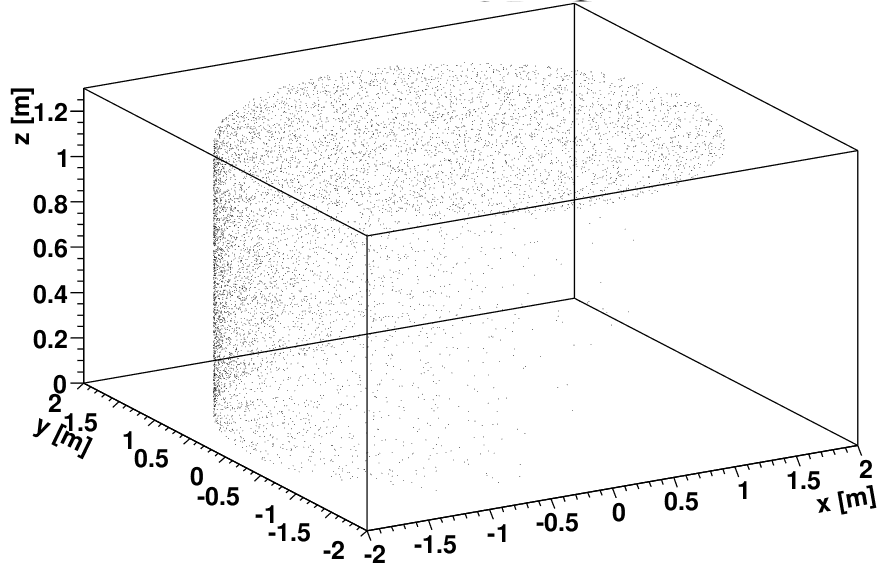
\includegraphics[width=0.7\textwidth]{fig/simulacionAuger/unthinning_tank}
			\caption{Distribuci\'on de part\'iculas sobre la superficie de un tanque luego de aplicar el algoritmo de unthinning.}
			\label{fig:unthinning_tank}
			\end{center}
		\end{figure}
		%
		
% 		En particular, el algoritmo de unthinning no es directamente aplicable a lluvias ES, por lo que una modificaci\'on del mismo se incluye en \Offline{} con el fin de resolver sus problemas.
		
% 		\textbf{RECTANGULOS ??}
		
		\subsubsection{Simulaci\'on del tanque}
		
		Para simular la respuesta del detector de superficie se ha incorporado en \Offline{} un m\'odulo especializado en la simulaci\'on del tanque basado en el paquete {\sc geant 4}~\cite{geant4}.
		
		{\sc geant 4} consiste en una librer\'ia de C++ que provee las herramientas necesarias para simular tanto la f\'isica como la geometr\'ia del detector.
		Algunas caracter\'isticas de dise\~no se exponen a continuaci\'on:
		\begin{itemize}
		\item Se procur\'o que todos los aspectos f\'isicos en esta etapa de la simulaci\'on sean lo m\'as precisos posible, mientras se trat\'o de tener buen entendimiento de su influencia en el resultado final.
		\item Por ser {\sc geant 4} una versi\'on m\'as sofisticada de programas anteriores, algunas de las variables del tanque fueron ajustadas de tal forma que los resultados experimentales se reproduzcan\footnote{Una de las m\'as importantes es la cantidad de fotoelectrones detectados por mu\'on vertical incidente.}.
% 		\item La velocidad de simulaci\'on es un factor importante.
% 		La simulaci\'on de estaciones cercanas al centro de la lluvia puede ser muy costosa debido a la gran cantidad de part\'iculas que se generan en esa regi\'on. Para evitar este inconveniente, se aplican cortes espec\'ificos en la producci\'on de fotones en el seguimiento de muones.
		\end{itemize}
		
		Por otro lado, a continuaci\'on se especifican algunos de los procesos f\'isicos tenidos en cuenta en la simulaci\'on del tanque:
		%
		\begin{itemize}
		\item La simulaci\'on de la propagaci\'on de una part\'icula cargada puede incluir efectos de ionizaci\'on, producci\'on de rayos delta, scattering de Coulomb múltiple, bremsstrahlung y radiaci\'on Cherenkov.
		\item Lor fotones producidos en la radiaci\'on Cherenkov (incluyendo los producidos por los rayos delta) son sometidos a scattering de Rayleigh, absorci\'on e interacci\'on \'optica con las paredes del tanque. La polarizaci\'on del fot\'on es tenida en cuenta siempre que es relevante.
		\end{itemize}
		%
		En particular, se encuentran especialmente modeladas y optimizadas las propiedades \'opticas de Tyvek, la longitud de absorci\'on del agua y la geometr\'ia de los PMTs.
		En la figura \ref{fig:cher_tank_sim} se muestra la simulaci\'on de los fotones Cherenkov generados en el pasaje de un electr\'on de baja energ\'ia a trav\'es del tanque.
		%
		\begin{figure}[h!]
			\begin{center}
			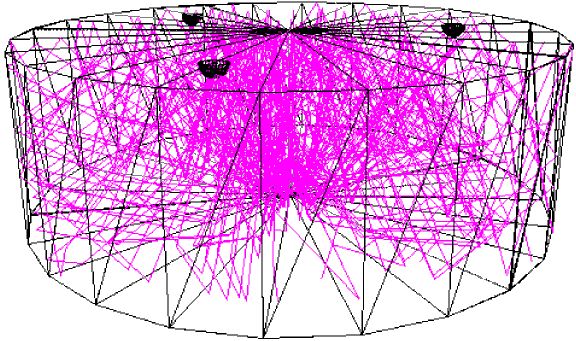
\includegraphics[width=0.7\textwidth]{fig/simulacionAuger/cher_tank_sim}
			\caption{Simulaci\'on de fotones Cherenkov generados en el pasaje de un electron de baja energ\'ia a trav\'es del tanque.}
			\label{fig:cher_tank_sim}
			\end{center}
		\end{figure}
		%
		
		Adem\'as de toda la f\'isica involucrada, la electr\'onica de la estaci\'on tambien es simulada.
		Luego de esta etapa, cada tanque involucrado en un evento tiene sus trazas FADC calculadas listas para ser analizadas por los algoritmos de trigger.
		
		\subsubsection{Trigger}
		
		Una vez que las trazas FADC fueron calculadas, \Offline{} posee algoritmos que calculan cada nivel de trigger del detector, desde disparos locales T2 hasta CDAS T4 y T5, especificados en la secci\'on \ref{sbsc:trig_levels}.
		
	\section{Librería de eventos generada}
	\label{sc:libGen}
	
	Para cada búsqueda se generó una librería de eventos que cubra todo el espacio de parámetros en el cual se esperan neutrinos que puedan generar lluvias que disparen el detector.
	
		\subsection{Eventos DGL}
		
		Para el canal CC se utilizaron energías fijas entre \cant{10^{17}}{eV} y \cant{10^{20.5}}{eV} con un paso logarítmico de $0.5$. 
		Dado que el canal NC sólo lleva el $20\%$ de la energía del neutrino, el rango energético fue acortado a \cant{10^{18}\ -\ 10^{20.5}}{eV}, evitando así simular eventos que no dispararían el detector.
		En canal double bang no fue tenido en cuenta, por lo que las lluvias iniciadas por \nutau{} se simularon como NC, subestimando así su eficiencia.
		En ambos canales, se simularon ángulos cenitales desde $60^\circ$ a $75^\circ$ con un paso de $3^\circ$, utilizando ángulos azimutales aleatorios entre $0^\circ$ y $360^\circ$.
		Con el fin de maximizar la eficiancia a la hora de simular se forzó a los neutrinos a interactuar en puntos de inyección de profundidad $D$, uniformemente distribuidos entre un valor máximo y un mínimo (que dependen del ángulo cenital) con un paso fijo de \cant{100}{g cm^{-2}}.
		Algunos puntos de inyección muy cercanos al suelo fueron omitidos debido a que la lluvia no llega a desarrollarse lo suficiente como para dar trigger.
		Para cada punto ($E_{\nu}$, $\theta$, $D$) se generaron 50 cascadas atmosféricas independientes.
		Cada una de estas se utilizó para producir cinco eventos con diferente punto de impacto en \Offline{}, dando un total de 250 eventos cuasi-independientes para cada punto de inyección.
		Todo lo anterior se resume en la tabla \ref{tab:sim_table_dgl}, mientras que la figura \ref{fig:sim_fig_dgl} muestra las profundidades simuladas como función del ángulo cenital.
		
		\begin{table}[ht]
			\begin{center}
			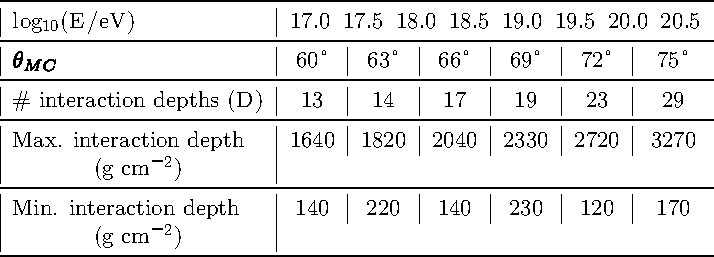
\includegraphics[width=0.85\textwidth]{fig/simulacionAuger/simShNavarro_1}
			\end{center}
			\caption{Resumen de las energías, ángulos cenitales y puntos de inyección. Para cada angulo, se simuló un número determinado de profundidades de interacción entre el máximo y un mínimo especificado en la tabla, con un paso de \cant{100}{g cm^{-2}}. Los dos primeros bines de energía no fueron simulados para el canal NC.
			}
			\label{tab:sim_table_dgl}
		\end{table}
		%
		\begin{figure}[h!]
			\begin{center}
			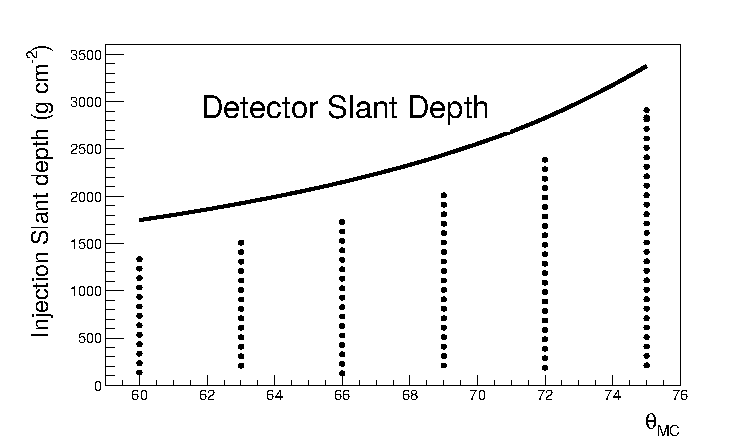
\includegraphics[width=0.85\textwidth]{fig/simulacionAuger/simShNavarro_2}\\
			\caption{En linea llena se grafica la prufundidad atmoférica inclinada del Observatorio Pierre Auger, que se encuentra a \cant{1400}{m} sobre el nivel del mar.
			Los circulos indican los puntos de inyección de los neutrinos (puntos de interacción) para diferentes ángulos cenitales.
			}
			\label{fig:sim_fig_dgl}
			\end{center}
		\end{figure}
		
		
		\subsection{Eventos DGH}
		
		La librería de eventos DGH fue obtenida con criterios muy similares a los utilizados en DGL, con la salvedad de que en este canal si se tuvieron en cuenta los eventos double bang.
		
		Con el fin de modelar las lluvias DB de manera fidedigna, se realizó la siguiente cadena de simulación:
	%
		\begin{enumerate}
		\item A partir de la simulación HERWIG de la primer interacción se obtuvo la energía transferida al leptón $\tau$ y las demás partículas producidas (jet hadrónico).
		\item Las partículas del jet hadrónico se inyectaron en \aires{} de manera análoga al procedimiento utilizado en la simulación de las lluvias producidas por $\nu_{e}$ vía CC o por $\nu_{X}$ vía CN. El leptón $\tau$ no se incluye en este grupo.
		\item Utilizando la energía transferida al leptón $\tau$ (dada por {\sc herwig}) se calculó la longitud de decaimiento y, mediante un MC simple, la distancia recorrida antes de decaer. La pérdida de energía en la atmósfera es despreciable y no se consideró en este cálculo.
		\item Si el resultado del punto anterior indicaba que el decaimiento se produjo antes de que el $\tau$ alcance la tierra, se utilizó el paquete {\sc tauola}~\cite{cite:TAUOLA} para calcular las partículas producidas en el decaimiento\footnote{{\sc tauola} es un MC desarrollado en el ambiente de altas energías que contiene toda la información experimental sobre los canales dominantes de dacaimiento del $\tau$. }.
		\item Los productos del decaimiento fueron inyectados en \aires{} a la profundidad y tiempo adecuados determinados por la distancia recorrida por el $\tau$.
		\item Se calculó la evolución conjunta de todas las partículas utilizando \aires{}.
		\end{enumerate}
		
		La tabla ~\ref{tab:sim_table_dgh} resume el conjunto de simulaciones producidas para este rango angular.
		\begin{table}[ht]
		\begin{center}
		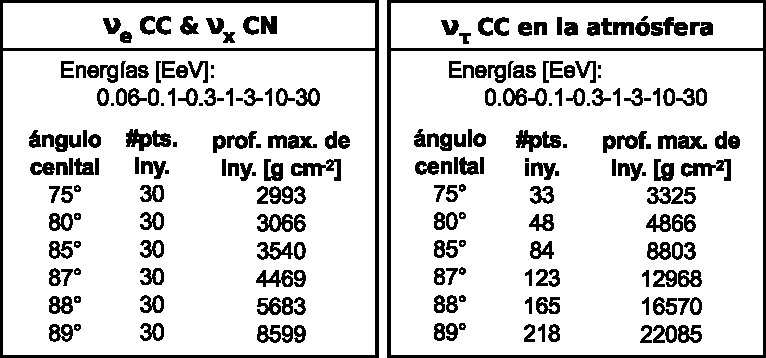
\includegraphics[width=0.75\textwidth]{fig/simulacionAuger/sim_table.pdf}
		\end{center}
		\caption{
		Resumen, discriminado por canal de interacción, de las simulaciones de neutrinos profundos realizadas.
		Para cada ángulo cenital se indica la profundidad de inyección máxima considerada (medida inclinada desde el detector) y la cantidad de puntos de inyección simulados en este rango. Las energías indicadas corresponden a la del neutrino primario.
		}
		\label{tab:sim_table_dgh}
		\end{table}
		Para cada ángulo cenital se indica la profundidad de inyección máxima considerada (medida inclinada desde el detector) y la cantidad de puntos de inyección simulados en este rango. Las energías indicadas corresponden a la del neutrino primario.
		
		\subsection{Eventos ES}
		
		En el caso de los eventos ES los parámetros que identifican una lluvia atmosférica son el ángulo cenital $\theta$, el ángulo azimutal $\Phi$, la energía del \tauon{} que escapa de la tierra \etau{} y la altura sobre el detector a la que el \tauon{} decae \xd{}.
		La energía del \tauon{} cubrió valores entre \cant{10^{16.5}}{eV} hasta \cant{10^{19.5}}{eV}, con paso de 0.5 logarítmico salvo en la zona de baja energía cuyo paso fue de 0.25.
		El ángulo cenital barrió valores desde $90.111^\circ$ hasta $95.884^\circ$ con paso de $0.573^\circ=0.1 \rm rad$ y en la zona de baja energía el ángulo máximo fue en algunos casos $93.549^\circ$.
		El ángulo azimutal $\Phi$ se eligió al azar entre $0^\circ$ y $360^\circ$.
		Con respecto a la altura de decaimiento \xd{} se utilizó un valor máximo que dependió de la energía del \tauon, y pasos de \cant{100}{m} o \cant{50}{m} para la zona de baja energía.
		Al igual que para los eventos DGH, para generar la libreria de eventos ES se simularon 50 eventos para cada punto ($\theta$,\etau{},\xd{}) y se utilizó cada lluvia 3 veces sobre el detector, logrando 150 eventos cuasi-independientes en cada caso. 
		La tabla \ref{tab:sim_table_es} condensa toda la información sobre las simulaciones ES, mientras que la figura \ref{fig:sim_fig_es} muestra los conjuntos de ($\theta$,\etau{},\xd{}) simulados.
		%
		\begin{table}
			\begin{center}
			\scriptsize
				\begin{tabular}{|c|c|cc|cc|}
				\hline
				\makebox[0.1\textwidth][c]{Group} & \makebox[0.13\textwidth][c]{\etau{} [eV]}&
				\makebox[0.15\textwidth][c]{\tita{} Min - Max} & \makebox[0.07\textwidth][c]{step [º]} & \makebox[0.13\textwidth][c]{\xd{} Min - Max} & \makebox[0.07\textwidth][c]{step [m]}\\
				\hline
				\hline
				\multirow{2}{*}{E003EeV} & \multirow{2}{*}{$3.16\times10^{16}$} & $95.884\text{ - }90.111$ & $0.573$ & $0\text{ - }600$ & $100$\\
				& & $93.549\text{ - }90.111$ & $0.573$ & $0\text{ - }300$ & $50$\\
				
				\multirow{2}{*}{E006EeV} & \multirow{2}{*}{$5.62\times10^{16}$} & \multirow{2}{*}{$93.549\text{ - }90.111$}  & \multirow{2}{*}{$0.573$} & \multirow{2}{*}{$0\text{ - }300$} & \multirow{2}{*}{$50$}\\
				& & & & &\\
				
				\multirow{2}{*}{E01EeV} & \multirow{2}{*}{$10^{17}$} & $95.884\text{ - }90.111$ & $0.573$ & $0\text{ - }700$ & $100$\\
				& & $93.549\text{ - }90.111$ & $0.573$ & $0\text{ - }300$ & $50$\\
				
				\multirow{2}{*}{E02EeV} & \multirow{2}{*}{$1.78\times10^{17}$} & \multirow{2}{*}{$93.549\text{ - }90.111$}  & \multirow{2}{*}{$0.573$} & \multirow{2}{*}{$0\text{ - }300$} & \multirow{2}{*}{$50$} \\
				& & & & &\\
				
				\multirow{2}{*}{E03EeV} & \multirow{2}{*}{$3.16\times10^{17}$} & $95.884\text{ - }90.111$ & $0.573$ & $0\text{ - }1000$ & $100$\\
				& & $93.549\text{ - }90.111$ & $0.573$ & $0\text{ - }300$ & $50$\\
				
				\multirow{2}{*}{E06EeV} & \multirow{2}{*}{$5.62\times10^{17}$} & \multirow{2}{*}{$93.549\text{ - }90.111$}  & \multirow{2}{*}{$0.573$} & \multirow{2}{*}{$0\text{ - }300$} & \multirow{2}{*}{$50$}\\
				& & & & & \\
				
				\multirow{2}{*}{E1EeV} & \multirow{2}{*}{$10^{18}$} & $95.884\text{ - }90.111$ & $0.573$ & $0\text{ - }1400$ & $100$ \\
				& & $93.549\text{ - }90.111$ & $0.573$ & $0\text{ - }300$ & $50$ \\
				
				\multirow{2}{*}{E3EeV} & \multirow{2}{*}{$3.16\times10^{18}$} & \multirow{2}{*}{$95.884\text{ - }90.111$}  & \multirow{2}{*}{$0.573$} & \multirow{2}{*}{$0\text{ - }1300$} & \multirow{2}{*}{$100$}\\
				& & & & & \\
				
				\multirow{2}{*}{E10EeV} & \multirow{2}{*}{$10^{19}$} & \multirow{2}{*}{$95.884\text{ - }90.111$}  & \multirow{2}{*}{$0.573$} & \multirow{2}{*}{$0\text{ - }1300$} & \multirow{2}{*}{$100$} \\
				& & & & & \\
				
				\multirow{2}{*}{E30EeV} & \multirow{2}{*}{$10^{19.5}$} & \multirow{2}{*}{$95.884\text{ - }90.111$}  & \multirow{2}{*}{$0.573$} & \multirow{2}{*}{$0\text{ - }2500$} & \multirow{2}{*}{$100$} \\
				& & & & &\\
				\hline
				\end{tabular}
			\end{center}
			\caption{\label{tab:sim_table_es}
			Detalle de los parámetros utilizados para generar la librería de eventos ES.
			}
		\end{table}
		%
		\begin{figure}[h!]
			\begin{center}
			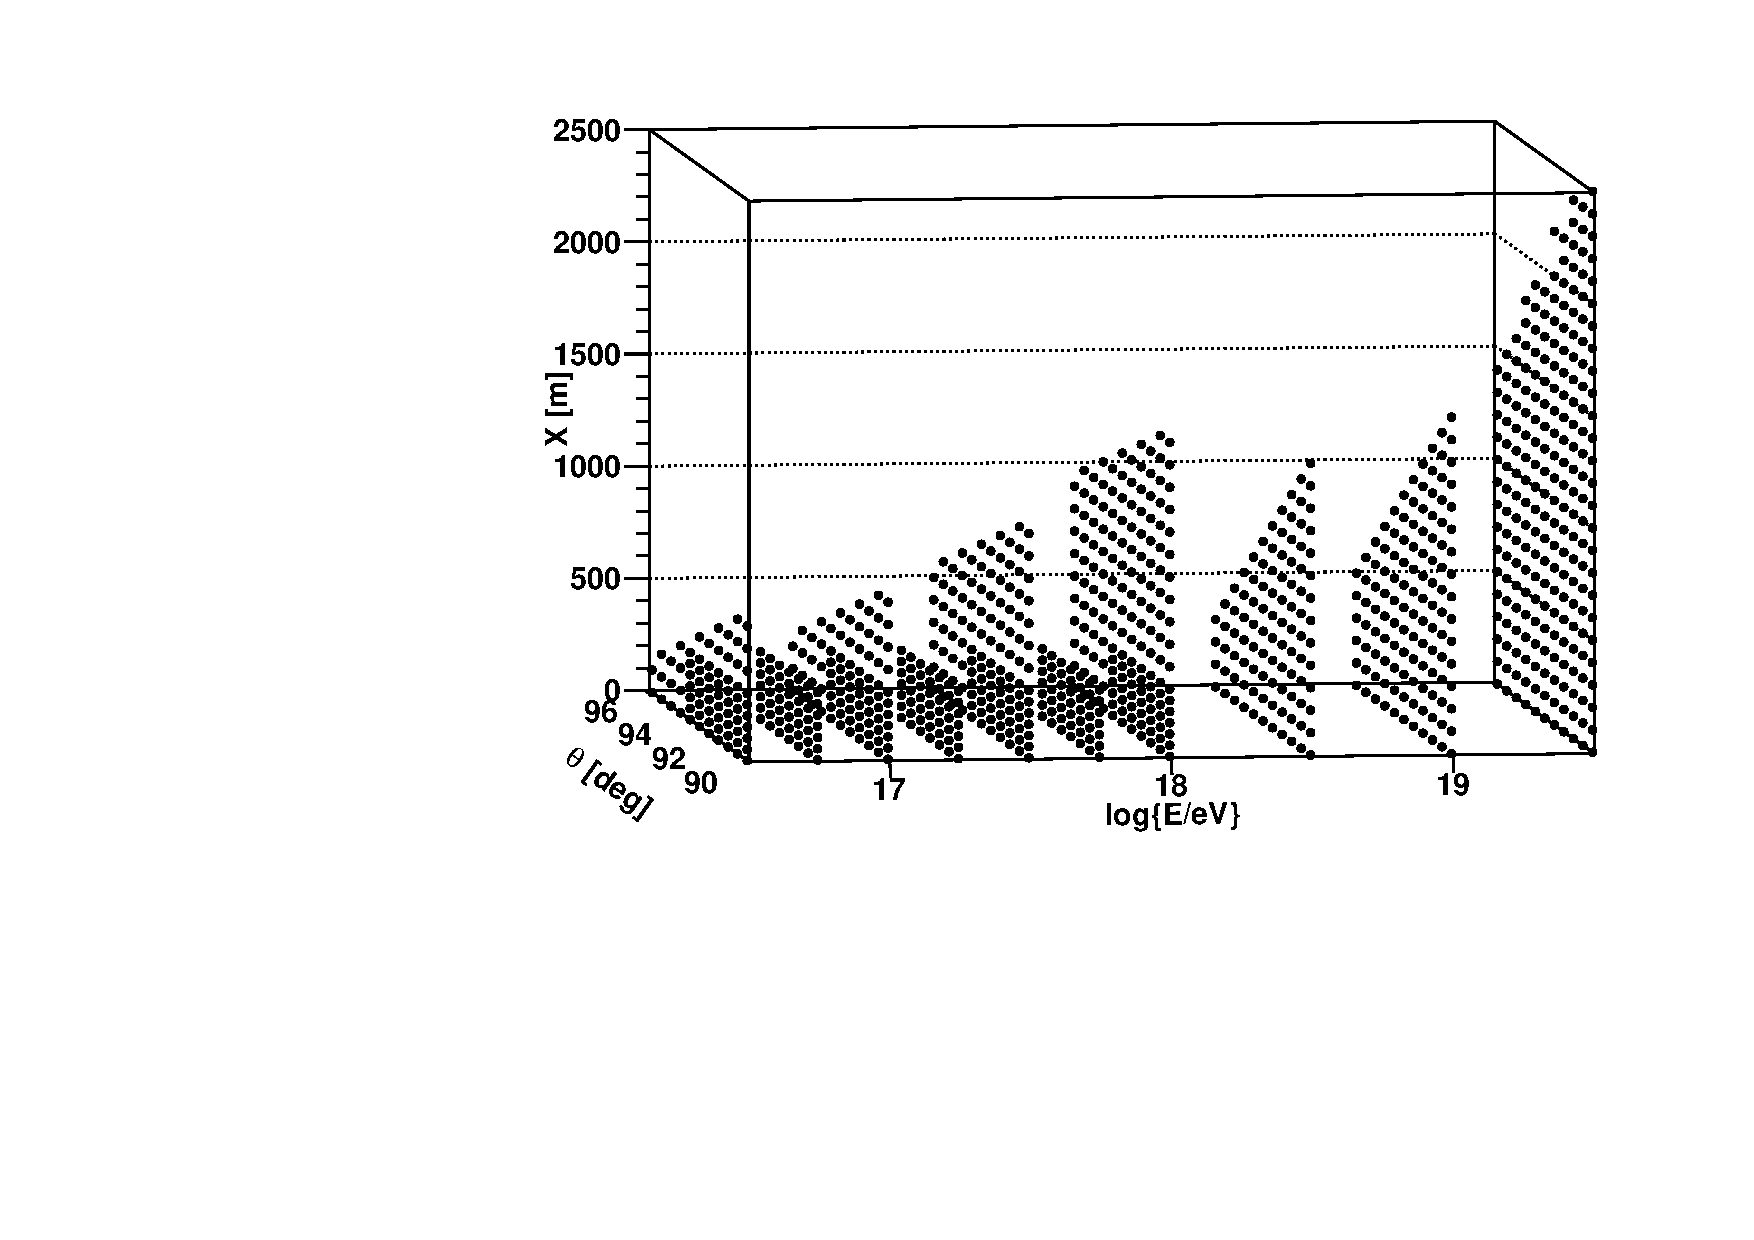
\includegraphics[width=0.85\textwidth]{fig/simulacionAuger/3D_completeParameterSpace5}
			\caption{
			Conjunto de ($\theta$,\etau{},\xd{}) utilizados para generar la librería de eventos ES.
			}
			\label{fig:sim_fig_es}
			\end{center}
		\end{figure}
		
	\section{Pesos de los eventos simulados}
	\label{sc:pesos}
	
	Si bien hasta el momento cada punto del espacio de parámetros, $(E_\nu,\theta,\phi,D)$ en DG y $(E_\tau,\theta,\phi,x_d)$ en ES, se encuentra bien representado, las frecuencia relativa con las que uno espera observarlos no suele ser la elegida a la hora de simular.
	Por este motivo, a la hora de poner a punto el método de selección será necesario corregir el peso de nuestra muestra simulada de tal manera que represente lo que realmente uno espera observar.
		
		\subsection{Correción en DG}
		
		Tal como se resume en la sección \ref{sub:neutrinoFlux}, se espera que el flujo difuso de neutrinos siga la forma $\Phi=k\cdot E^{-2}$. Por otro lado la, la sección eficaz $\nu$-nucleón crece, de manera aproximada, como $E^{1/3}$~\cite{cite:cooper_sarkar}.
		La dependencia del peso con el ángulo cenital surge de la proyección del área del detector en la dirección del flujo incidente (ver sección \ref{sc:expoNu} más adelante para una explicación detallada) y de que el paso en los ángulos simulados no es constante.
		Por último es necesario tener en cuenta que dado que la sección eficaz de los neutrinos es muy pequeña, su rango en la atmósfera es muy grande.
		Por esto es una buena aproximación considerar que todos las profundidades $D$ son igual de probables.
		Uniendo los ingredientes anteriores se obtiene:
		%
		\begin{equation}
		w(E_\nu,\theta) \propto \cos\theta \sin\theta \, E^{-2/3} \Delta\theta
		\end{equation}
		%
		que se utiliza para definir la importancia relativa entre los eventos simulados.
		
		\subsection{Corrección en ES}
		
		El caso de las lluvias ES es bastante más complicado dado que los parámetros que nos interesa corregir son $(E_\tau,\theta,\phi,x_d)$.
		Por esto, además de la dependencia con el ángulo sólido, es necesario incluir la probabilidad de que el \tauon{} escape de la tierra con cierta energía y decaiga a cierta altura.
		Entonces, para construir los pesos de los eventos ES puede escribirse:
		%
		\begin{equation}
		 w(E_\tau,\theta,x_d) \propto \int_{E_\tau}^\infty \Phi(E_\nu)dE_\nu f(E_\tau|E_\nu,\theta) h(x_d,(E_\tau,\theta)) E_\tau \Delta\log E_\tau \Delta x_d
		 \label{eq:wi}
		\end{equation}
		%
		donde la integral aparece porque deben tenerse en cuenta todos los \nutau{}'s que pueden generar un \tauon{} de energía \etau{}.
		La aparición de los términos $E_\tau \Delta\log E_\tau \Delta x_d$ se debe nuevamente a que lis bines simulados no se encuentran uniformemente distribuidos en las variables $(E_\tau,x_d)$.
		Al igual que para las lluvias DG, el flujo difuso de neutrinos se supone $\Phi=k\cdot E^{-2}$.
		La función $h(x_d,(E_\tau,\theta))$ corresponde a la probabilidad de que un \tauon{} de parámetros $(E_\tau,\theta)$ decaiga a una altura $x_d$ del detector, y tiene la forma:
		%
		\begin{equation}
		 h(x_d,(E_\tau,\theta))=
		 \exp{\left(
		 -\frac{l(x_d,\theta)}{\lambda(E_\tau)}
		 \right)}
		 \frac{dl}{dx_d}\frac{1}{\lambda(E_\tau)}
		\end{equation}
		%
		donde $\lambda(E_\tau)=c\uptau\frac{E_\tau}{m_\tau}\sim49\left(\frac{E_\tau}{\rm EeV}\right){\rm km}$ y $l(x_d,\theta)=\frac{x_d}{|\cos\theta|}$, quedando:
		\begin{equation}
		 h(x_d,(E_\tau,\theta))=
		 \exp{\left(
		 -\frac{x_d}{|\cos\theta|\lambda(E_\tau)}
		 \right)}
		 \frac{1}{|\cos\theta|\lambda(E_\tau)}
		 \label{eq:ptaudecay}
		\end{equation}
		%
		
		En la ecuación \ref{eq:wi} la parte complicada reside en $f(E_\tau|E_\nu,\theta)$, que corresponde a la probabilidad de que dado un neutrino de energía $E_\nu$ y ángulo $\theta$ emerja de la tierra un \tauon{} de energía \etau{}.
		Para obtener estas probabilidades es necesario recurrir a simulaciones, lo que se detalla a continuación.
		
		\subsubsection{\label{sbsbsc:sim_prop_tierra}Propagaci\'on dentro de la tierra}
	
		Para simular la interacción del \nutau{} y propagaci\'on del \tauon{} en la tierra se utiliz\'o un programa que realiza el c\'alculo mediante m\'etodos de Monte Carlo. Este fue desarrollado por J. A. Mu\~niz y E. Zas, del grupo de altas energ\'ias de la Universidad de Santiago de Compostela.
		Una explicaci\'on detallada del programa puede encontrarse en \cite{gap_tau_tierra}.
		
		Este c\'odigo permite propagar los \nutau{}s y \tauon{}s en la tierra y, dado el \'angulo cenital \tita{} y la energ\'ia del neutrino incidente \enu{}, calcular la probabilidad de que un \tauon{} alcance la superficie de la tierra con energ\'ia \etau{}.
		Estos c\'alculos se realizan teniendo en cuenta la interacci\'on del \nutau{} via CC y CN, la p\'erdida de energ\'ia del \tauon{} (con $\beta$\footnote{ver ecuaci\'on \ref{eq:tau_losses}} dependiente o independiente de la energ\'ia) y la regeneraci\'on del flujo de \nutau{} debido a interacciones via CN y a decaimientos de leptones \tauon{}.
		
		La simulaci\'on consta de dos etapas principales que se alternan hasta que se alcanza la superficie:
		%
		\begin{description}
		\item[\textbf{Interacci\'on del \nutau{}:}] Se hace interactuar al neutrino siguiendo una distribuci\'on exponencial en $x$, donde $x$ es la variable que mide la cantidad de materia atravesada por el \nutau{}. Para ello, se tienen en cuenta interacciones via CC y CN. Si se diera una interacci\'on via CC, se produce un \tauon{} cuya energ\'ia proviene de muestrear la sección efic\'az diferencial de CC, $\frac{d\sigma^{cc}}{dy}$. En cambio, si la interacci\'on se produce via CN, es generado un nuevo \nutau{} de energ\'ia menor que se hace interactuar nuevamente.
		\item[\textbf{Propagaci\'on del \tauon{}:}] En caso de que un \tauon{} sea producido, se lo propaga de a peque\~nos pasos, calculando en cada uno de ellos la energ\'ia perdida debido a la interacci\'on con el medio y la probabilidad de decaimiento (como funci\'on de su energ\'ia). Si decayese produciendo un nuevo \nutau{}, se comienza el procedimiento nuevamente desde el punto del \'ultimo decaimiento.
		\end{description}
		%
		Este proceso se esquematiza en la figura \ref{fig:tau_sim_sch}.
		\begin{figure}[ht!]
			\begin{center}
			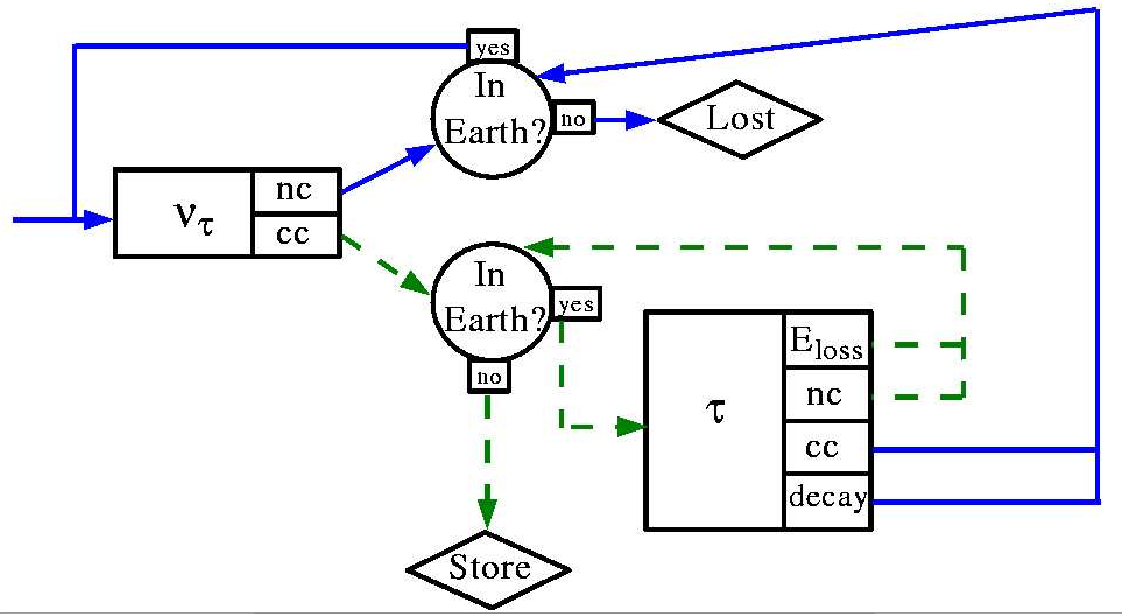
\includegraphics[width=0.75\textwidth]{fig/simulacionAuger/schemeEarthProp}
			\caption{\label{fig:tau_sim_sch} Esquema del algoritmo de simulación de las interacción en la tierra. El \nutau{} (línea sólida) y el \tauon{} (línea punteada) son simulados hasta que abandonan la tierra. La salida del algoritmo es un histograma de energía de los \tauon{} salientes.}
			\end{center}
		\end{figure}
		
		El programa fue validado utilizando programas mucho m\'as complejos, como ANIS \cite{anis}.
		Tambi\'en se realiz\'o una comparaci\'on del flujo de \tauon{} saliente obtenido mediante el calculo te\'orico que puede encontrarse en \cite{prop_tau} y el obtenido por este programa, para diferentes \'angulos cenitales.
		Esta \'ultima comparaci\'on se muestra en la figura \ref{fig:comp_tau_mc_teo}, en la que se observa un muy buen acuerdo entre ambos resultados.
		%
		\begin{figure}[ht!]
			\begin{center}
			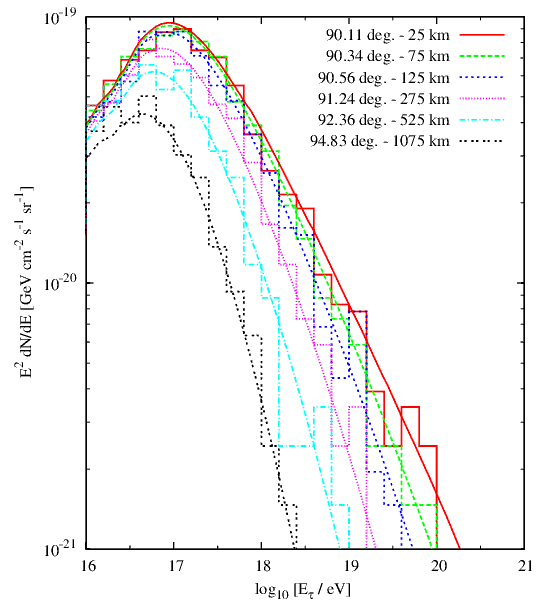
\includegraphics[width=0.55\textwidth]{fig/simulacionAuger/comp_tau_mc_teo}
			\caption{\label{fig:comp_tau_mc_teo} Comparaci\'on de los flujos salientes obtenido anal\'iticamente y mediante simulaci\'on. Los histogramas corresponden a los resultados del Monte Carlo, mientras que la l\'inea llena al c\'alculo te\'orico.}
			\end{center}
		\end{figure}
		
		
		Una vez obtenidos todos los términos de la ecuación \ref{eq:wi}, la integral se realiza numericamente.
\chapter{Reconstrucci\'on de los eventos  y selecci\'on de eventos candidatos}
\label{ch:selAuger}

En este capítulo se describe la metodología aplicada para elegir el criterio de selección en las tres búsquedas.
En primer lugar se definen cortes de calidad que eliminan estaciones o incluso eventos espúreos, con el fin de lograr una reconstrucción confiable.
Una vez hecho esto se utilizan variables topológicas y temporales para elegir eventos inclinados, y luego  se agrega información de las trazas para seleccionar las lluvias jóvenes.

\section{Criterios de calidad}

	Al inicio de la cadena de procesamiento se cuenta con un conjunto de eventos que cumplen el criterio de trigger T3.
	De este grupo, se eliminan en primer lugar los datos que se hayan tomado en períodos en los que el detector se haya comportado de manera inestable.
	Luego, se aplica a cada evento una serie de procedimientos que se mencionan a continuación:
	\begin{itemize}
	 \item Selección de tubos fotomultiplicadores (PMT's)
	 \item Selección de estaciones
	 \item Reconstrucción preeliminar
	 \item Cortes adicionales
	\end{itemize}
	
	\subsection{Selección de tubos fotomultiplicadores}
	
	La búsqueda de neutrinos consiste en encontrar eventos extremadamente raros en el detector, por lo que en caso de aparecer algun candidato, es de extrema importancia que todas sus estaciones posean PMT's que funcionen correctamente.
	En particular es vital descartar los PMT's que posean patologías que alarguen la señal en el tiempo, ya que, como se verá en la sección \ref{sc:selNu}, la selección de lluvias jóvenes depende fuertemente de este factor.
	
	Hay varios cortes que se utilizan para descartar PMT's. 
	Estos pueden ser separados en dos grupos, que se describen a continuación.
	
		\subsubsection{Criterios basados en la integral de la señal}
		
		Este conjunto de cortes es el resultado de estudios \cite{pmtsAuger} llevados a cabo por el grupo de monitoreo del observatorio. 
		A partir de estos estudios se provee una lista de PMT's inestables día a día.
		Los parámetros que son estudiados para definir esta clasificación son las líneas de base del ánodo y del dínodo, y el llamado relación entre el dínodo y el ánodo (dínodo/ánodo).
		
		En el caso de las líneas de base se requiere que sus fluctuaciones sean pequeñas, mediante un corte en su RMS. Para la relación dínodo/ánodo además se utilizan dos cortes que limitan su valor máximo y mínimo.
		
		La figura \ref{fig:event1634332} se muestra un ejemplo en el que el PMT número 3 es descartado debido a que posee una relación dínodo/ánodo más pequeña que la permitida, mientras que las otras dos estaciones muestran valores normales.
		
		 \begin{figure}[h!]
			\begin{center}
			$
			\begin{array}{cc}
			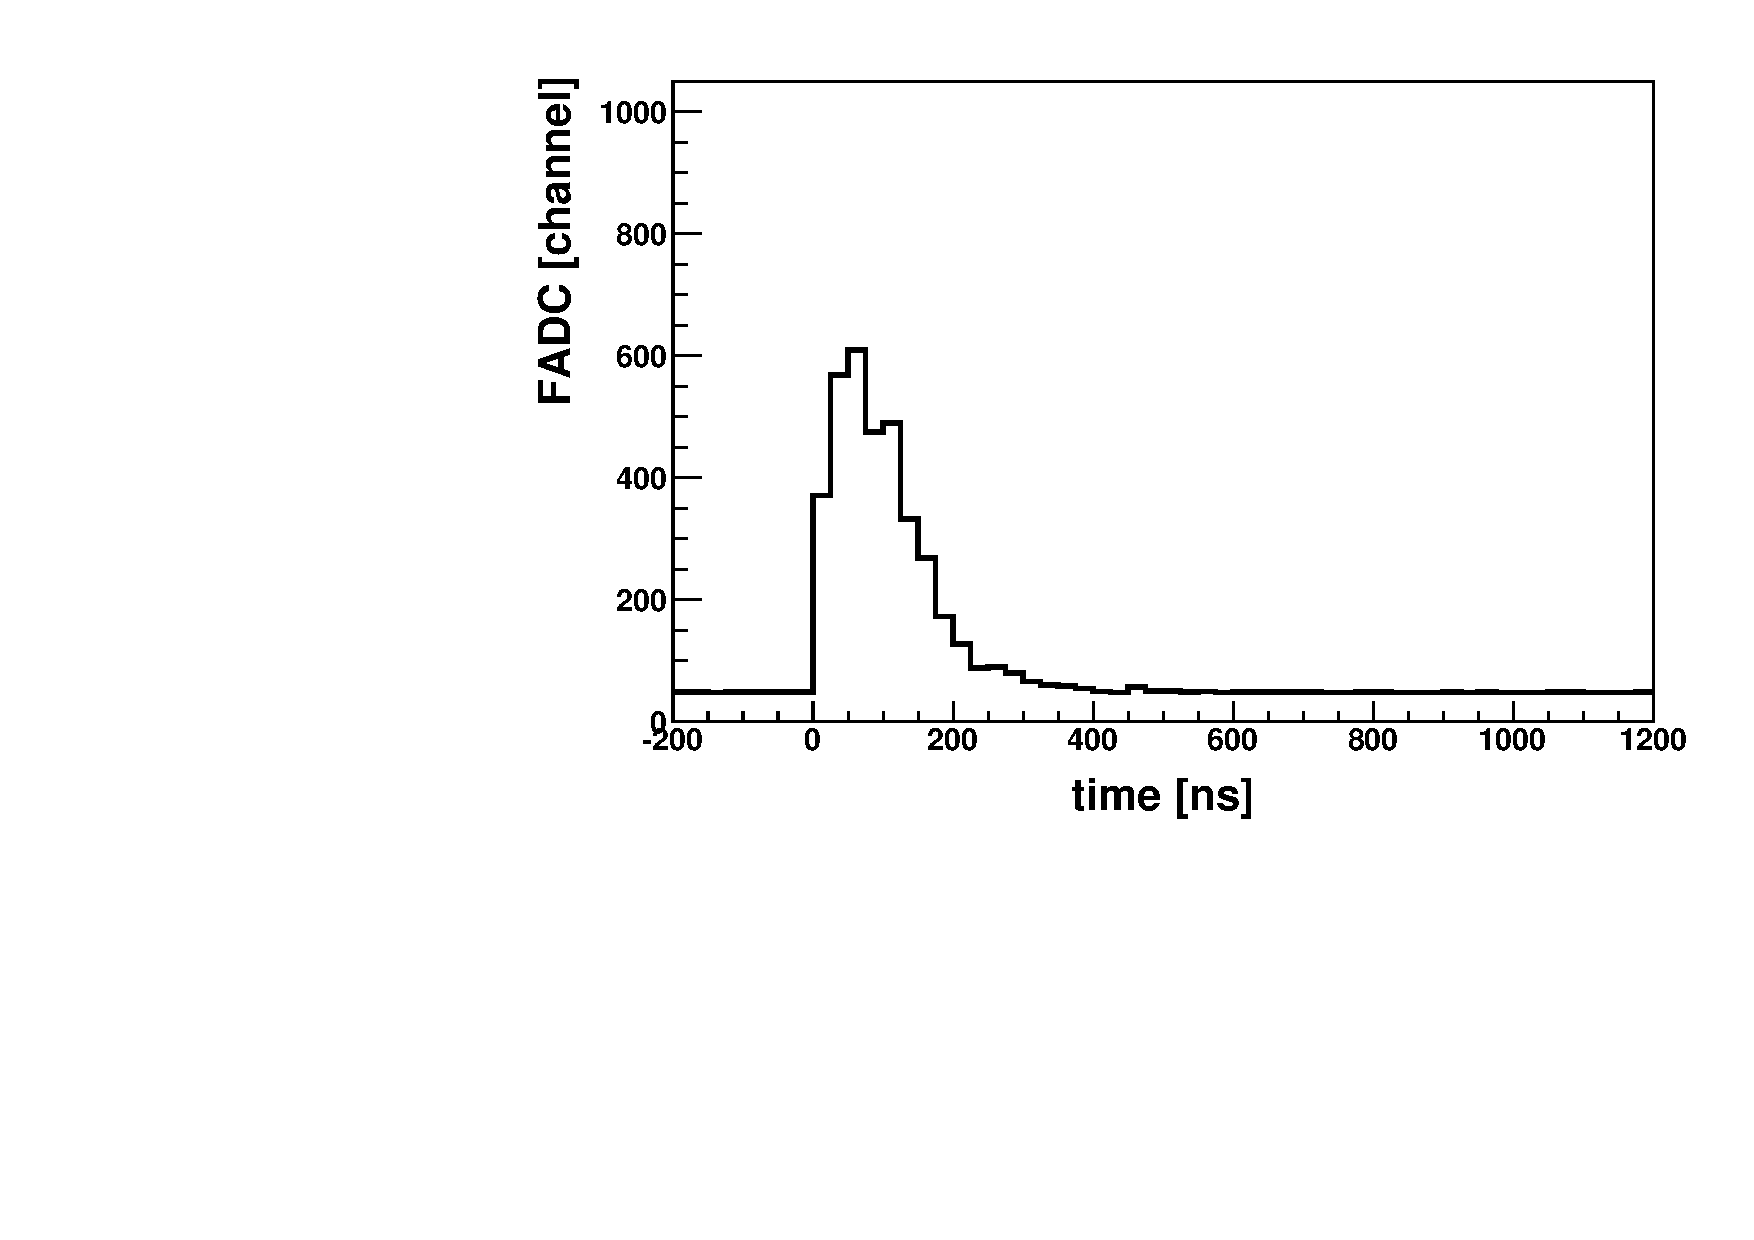
\includegraphics[width=0.47\textwidth]{fig/seleccionAuger/ev1634332_pmt1_anode.pdf} & 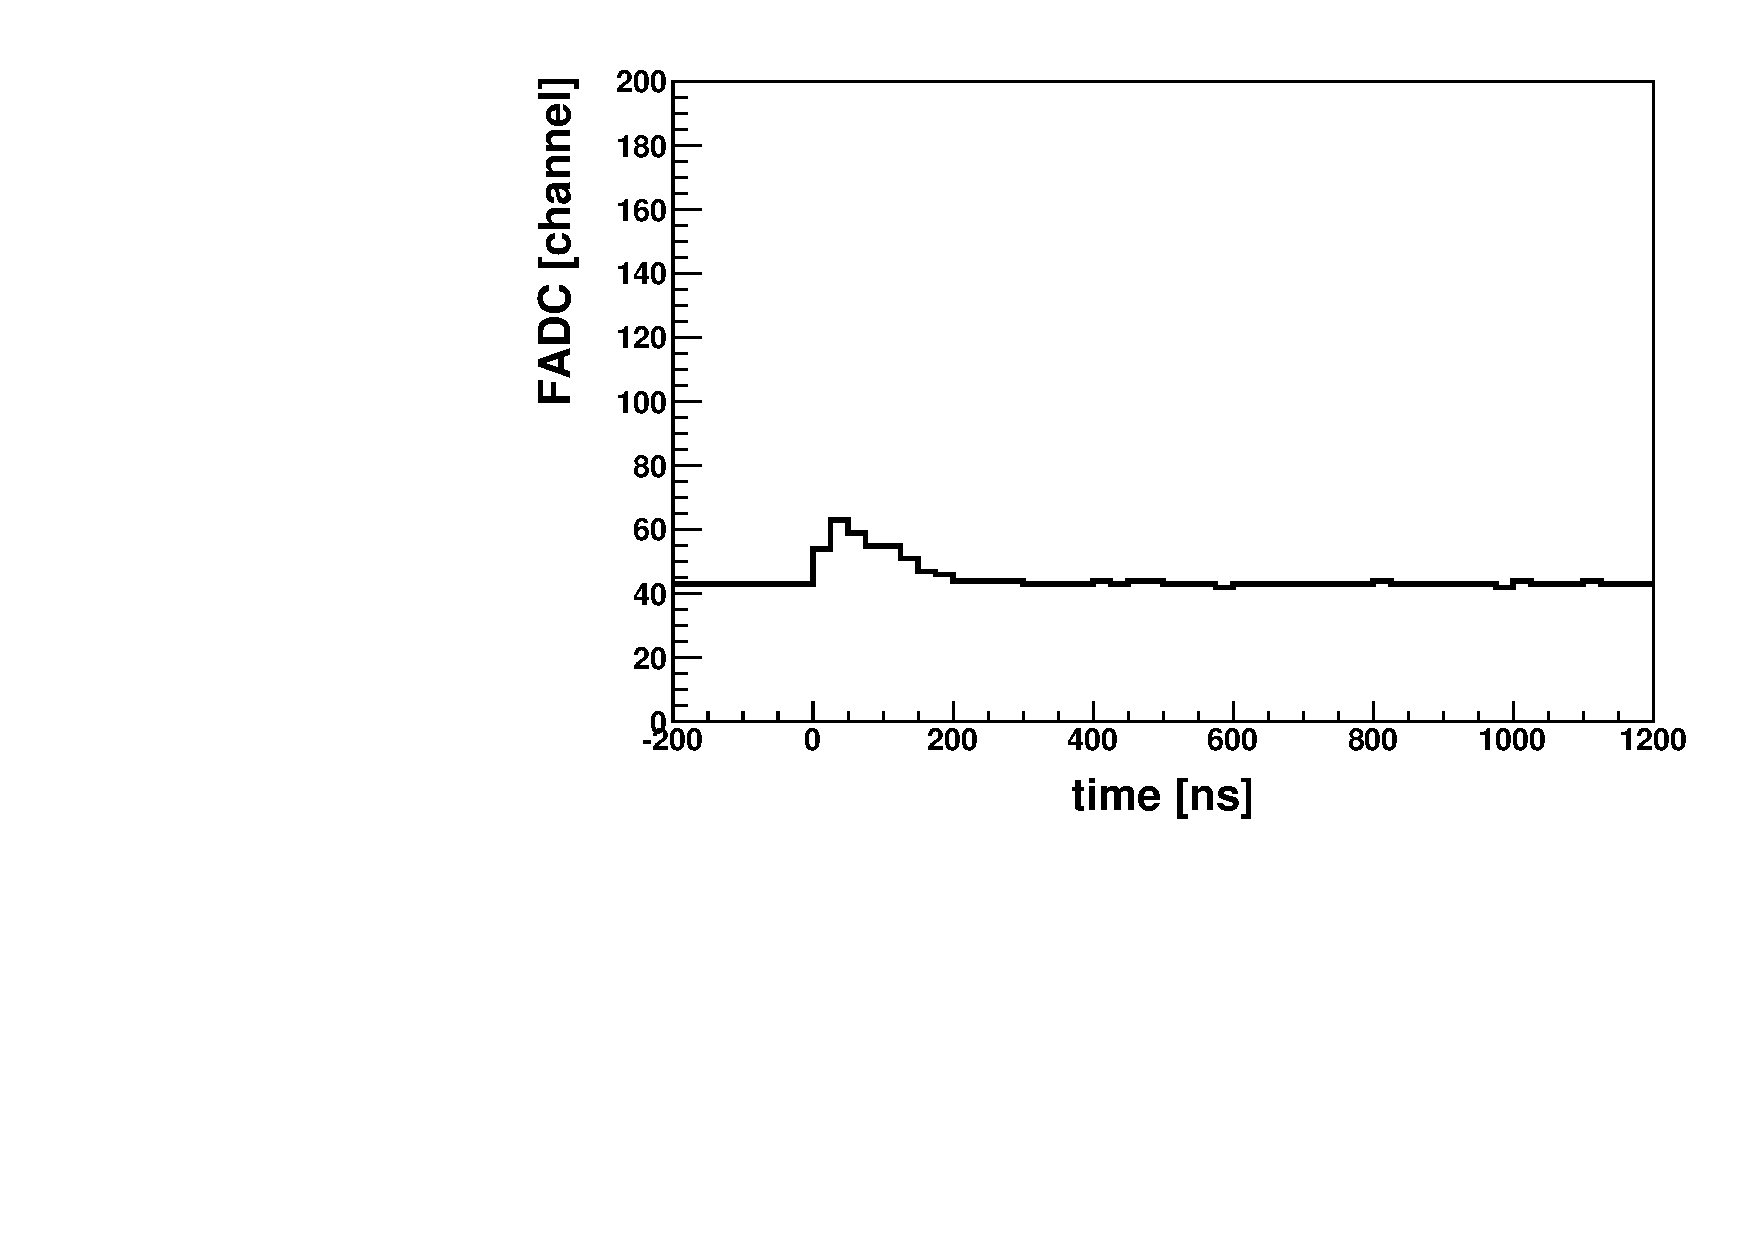
\includegraphics[width=0.47\textwidth]{fig/seleccionAuger/ev1634332_pmt1_dynode.pdf}\\
			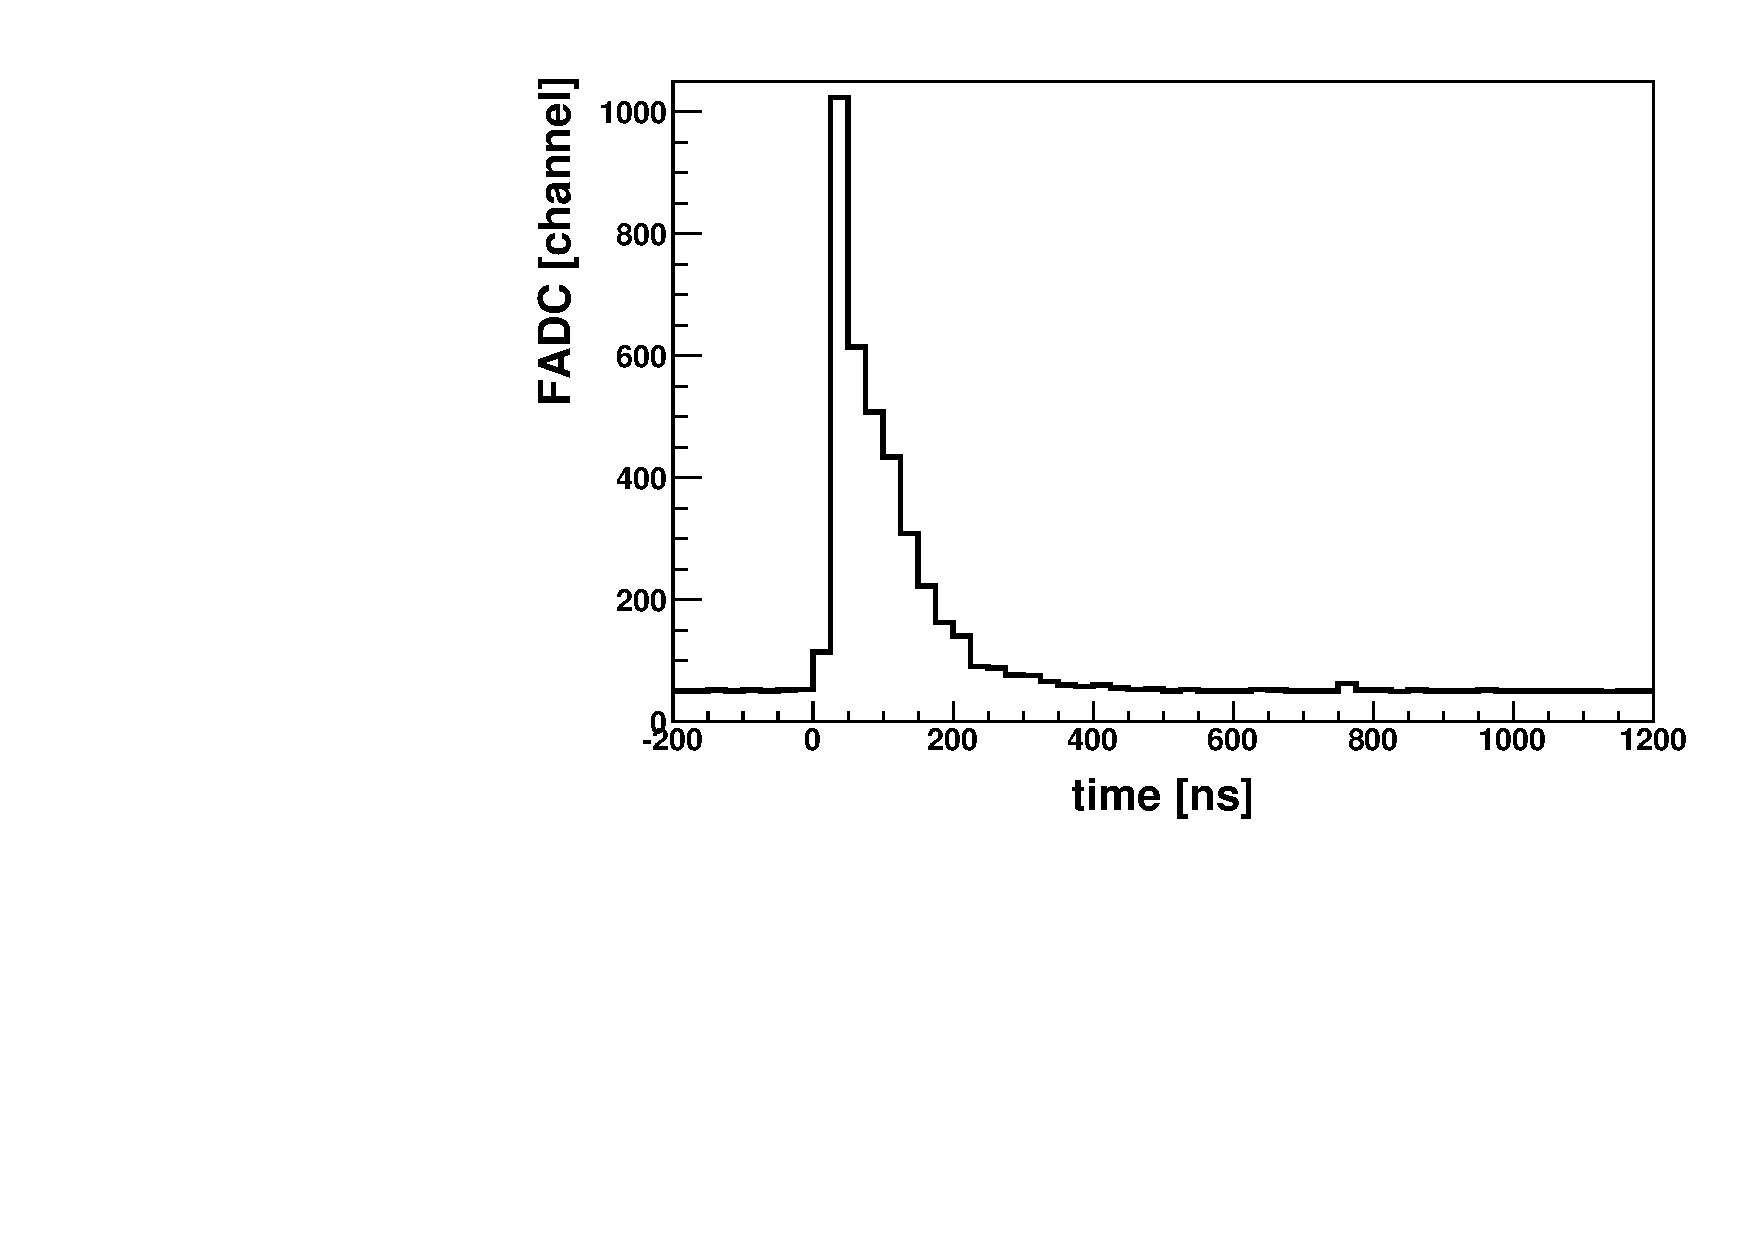
\includegraphics[width=0.47\textwidth]{fig/seleccionAuger/ev1634332_pmt2_anode.pdf} & 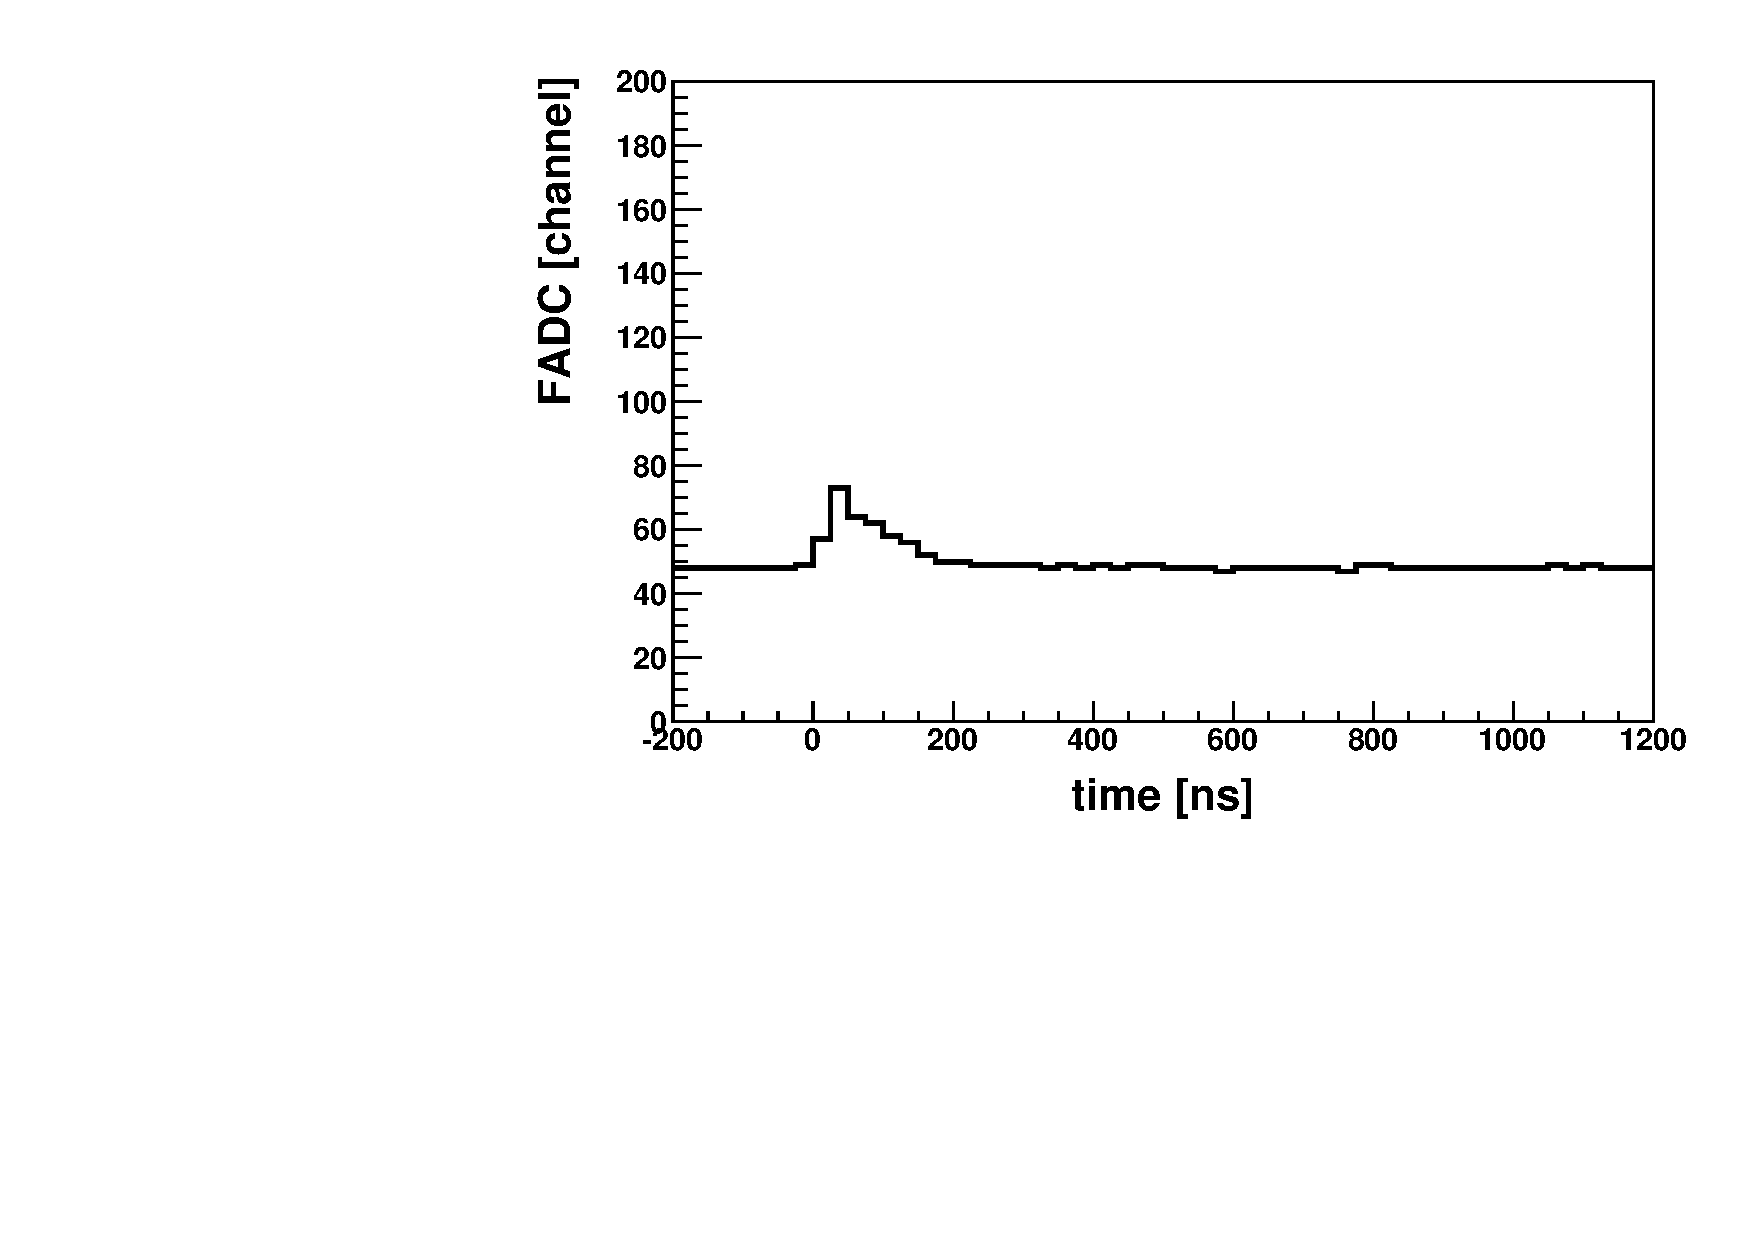
\includegraphics[width=0.47\textwidth]{fig/seleccionAuger/ev1634332_pmt2_dynode.pdf}\\
			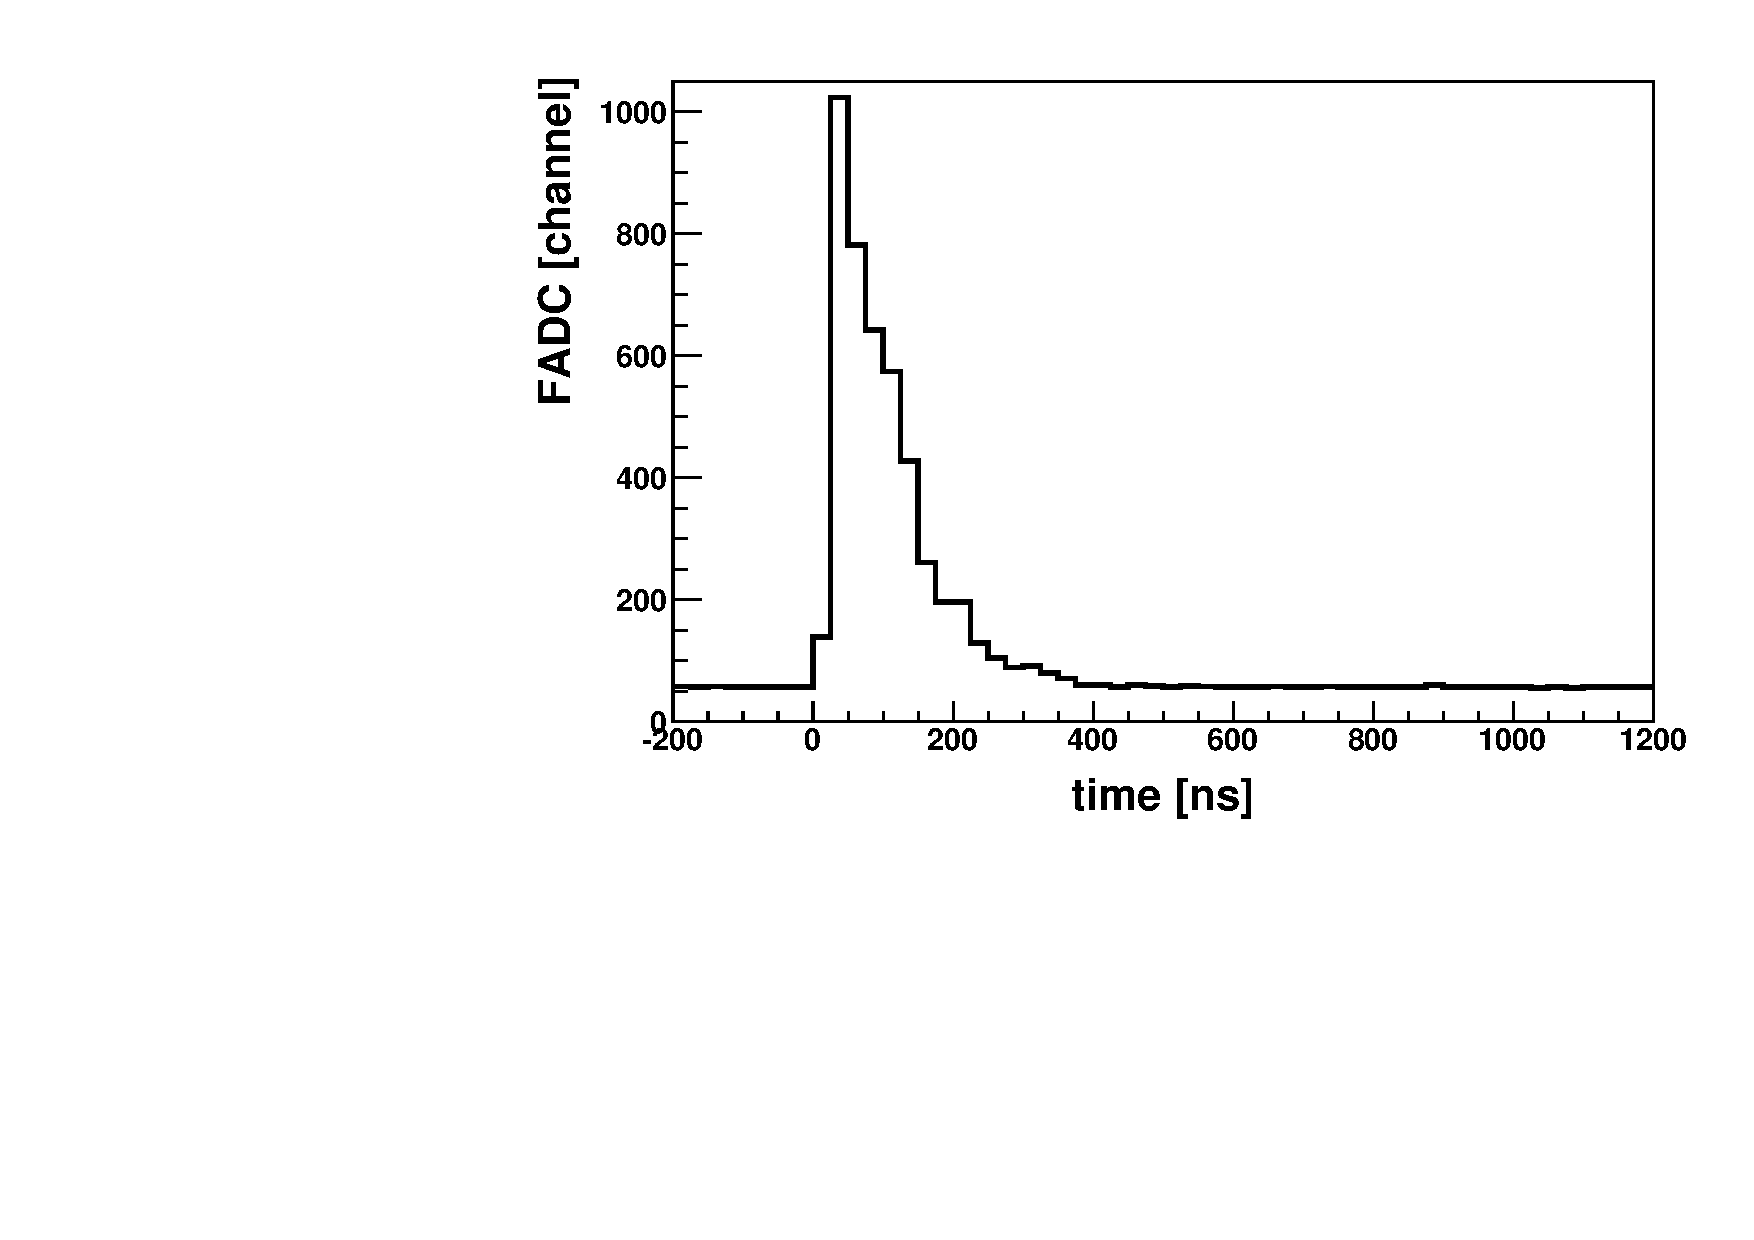
\includegraphics[width=0.47\textwidth]{fig/seleccionAuger/ev1634332_pmt3_anode.pdf} & 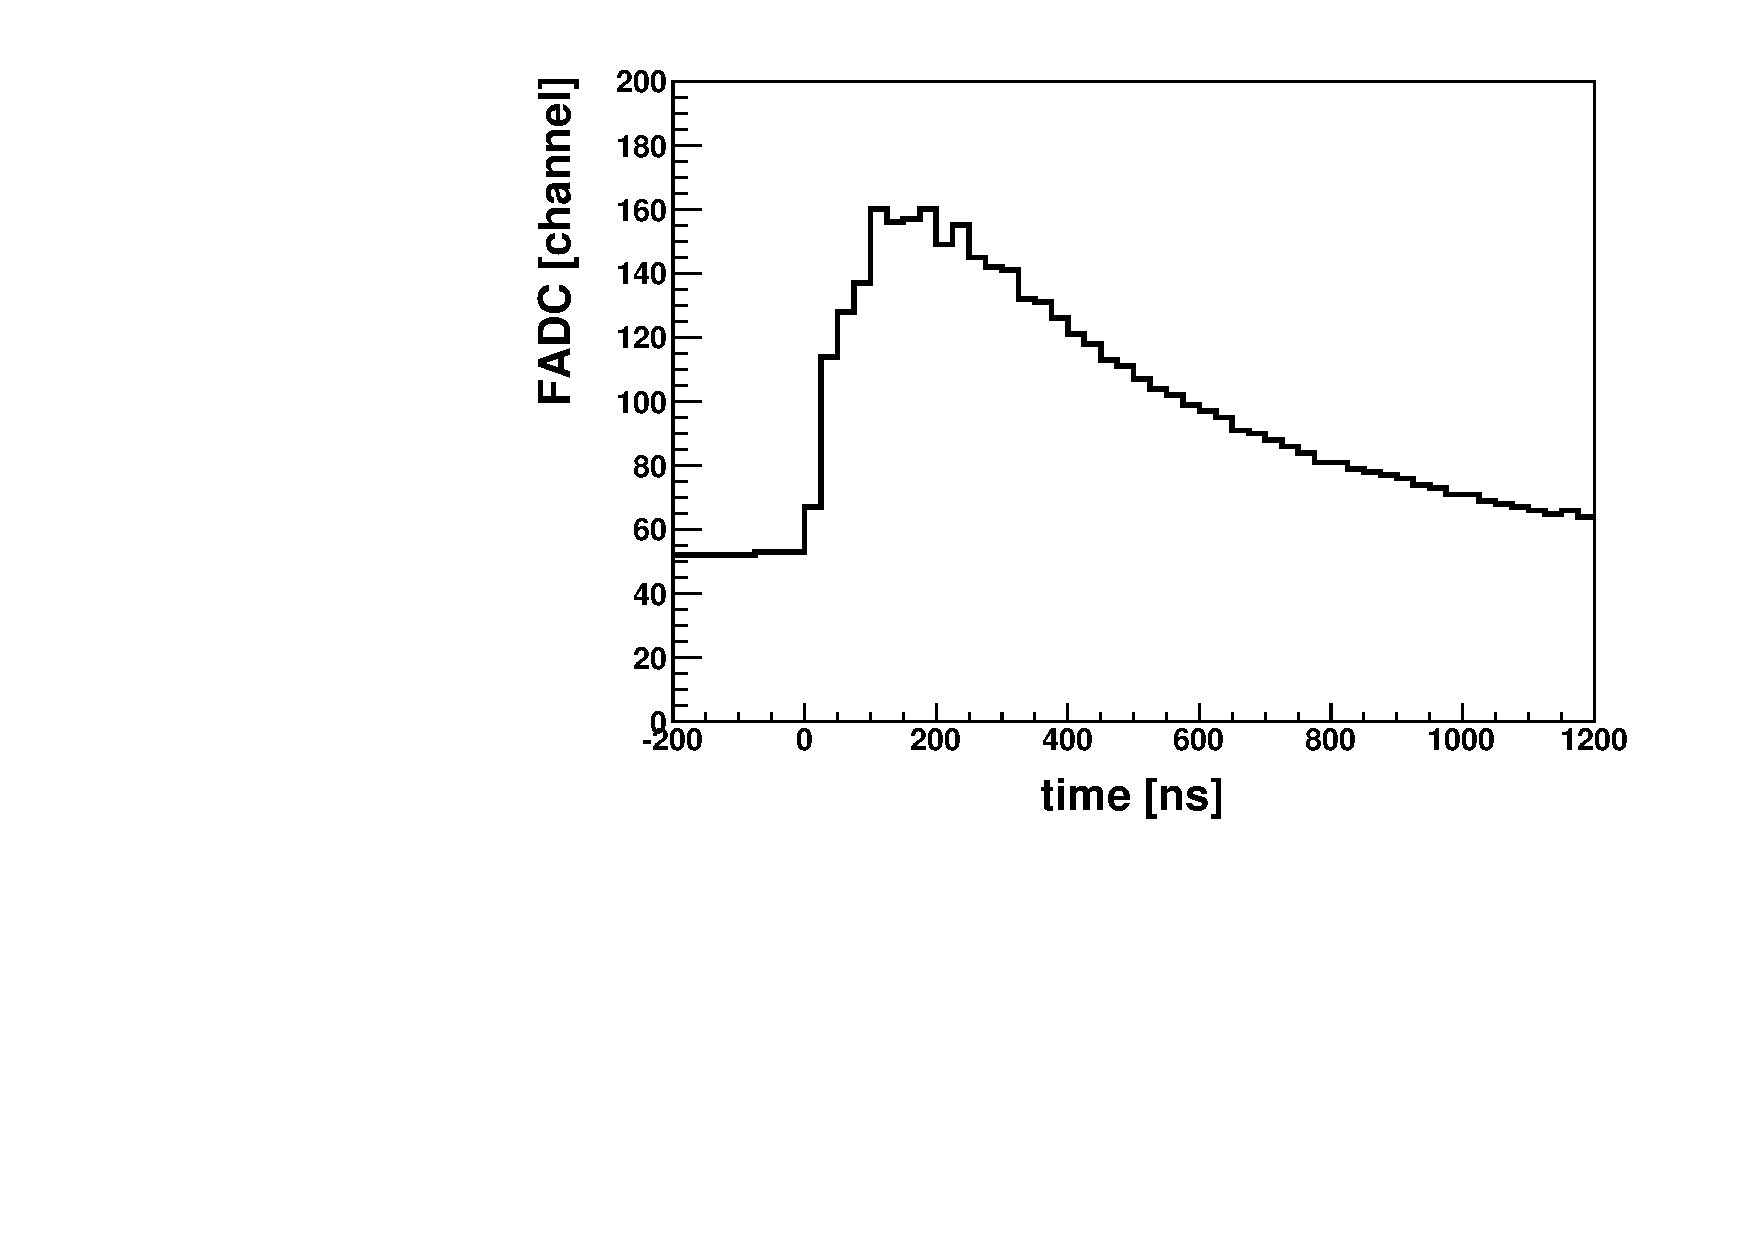
\includegraphics[width=0.47\textwidth]{fig/seleccionAuger/ev1634332_pmt3_dynode.pdf}\\
			\end{array}
			$
			\caption{Ejemplo de un PMT descartado. 
			Estación número 717 (Bobik) en el evento 1634332 detectado el 19 de Septiembre de 2005.
			De arriba hacia abajo PMT's de 1 a 3.
			En la columba izquierda (derecha) se muestra la FADC del ánodo (dínodo).
			El PMT's 3 es rechazado por tener la relación dínodo/ánodo pequeña.
			}
			\label{fig:event1634332}
			\end{center}
		\end{figure}
		
		
		\subsubsection{Criterios basados en la forma de la señal}
		
		Cuando además de la integral de la señal se presta atención a la forma de la misma, otro tipo de patologías salen a la luz, la mayoría de las veces dando lugar a un exceso de señal en la traza.
		
		Para detectar este tipo de PMT's prblemáticos se diseñó un procedimiento especial, que se detalla a continuación:
		\begin{enumerate}
		 \item Se calculan las integrales de las señales en el dínodo correspondientes a la última mitad de la traza ($\Sigma_i$, con $i$ corriendo sobre los PMT's).
		 \item Se descuenta a cada $\Sigma_i$ el bin de mayor señal y su entorno, para eliminar pulsos generados por muones accidentales.
		 \item Se etiqueta un PMT como dudoso si se cumple:
		 \begin{itemize}
		  \item La estación posee al menos dos PMT's activos.
		  \item El máximo $\Sigma_i$ es mayor a \cant{4}{VEM} y al menos 7 veces mayor que el resto.
		 \end{itemize}
		\end{enumerate}
		
		Si determinado PMT es estiquetado como dudoso durante un período de tiempo largo se lo considera un indicador de que presenta mal funcionamiento y se lo descarta.
		
		La figura \ref{fig:event3995196} muestra un ejemplo de este comportamiento. 
		
		\begin{figure}[h!]
			\begin{center}
			$
			\begin{array}{cc}
			%  \raisebox{0.8\height}{\includegraphics[width=0.4\textwidth]{fig/mapEvent1634332.png}} & 
			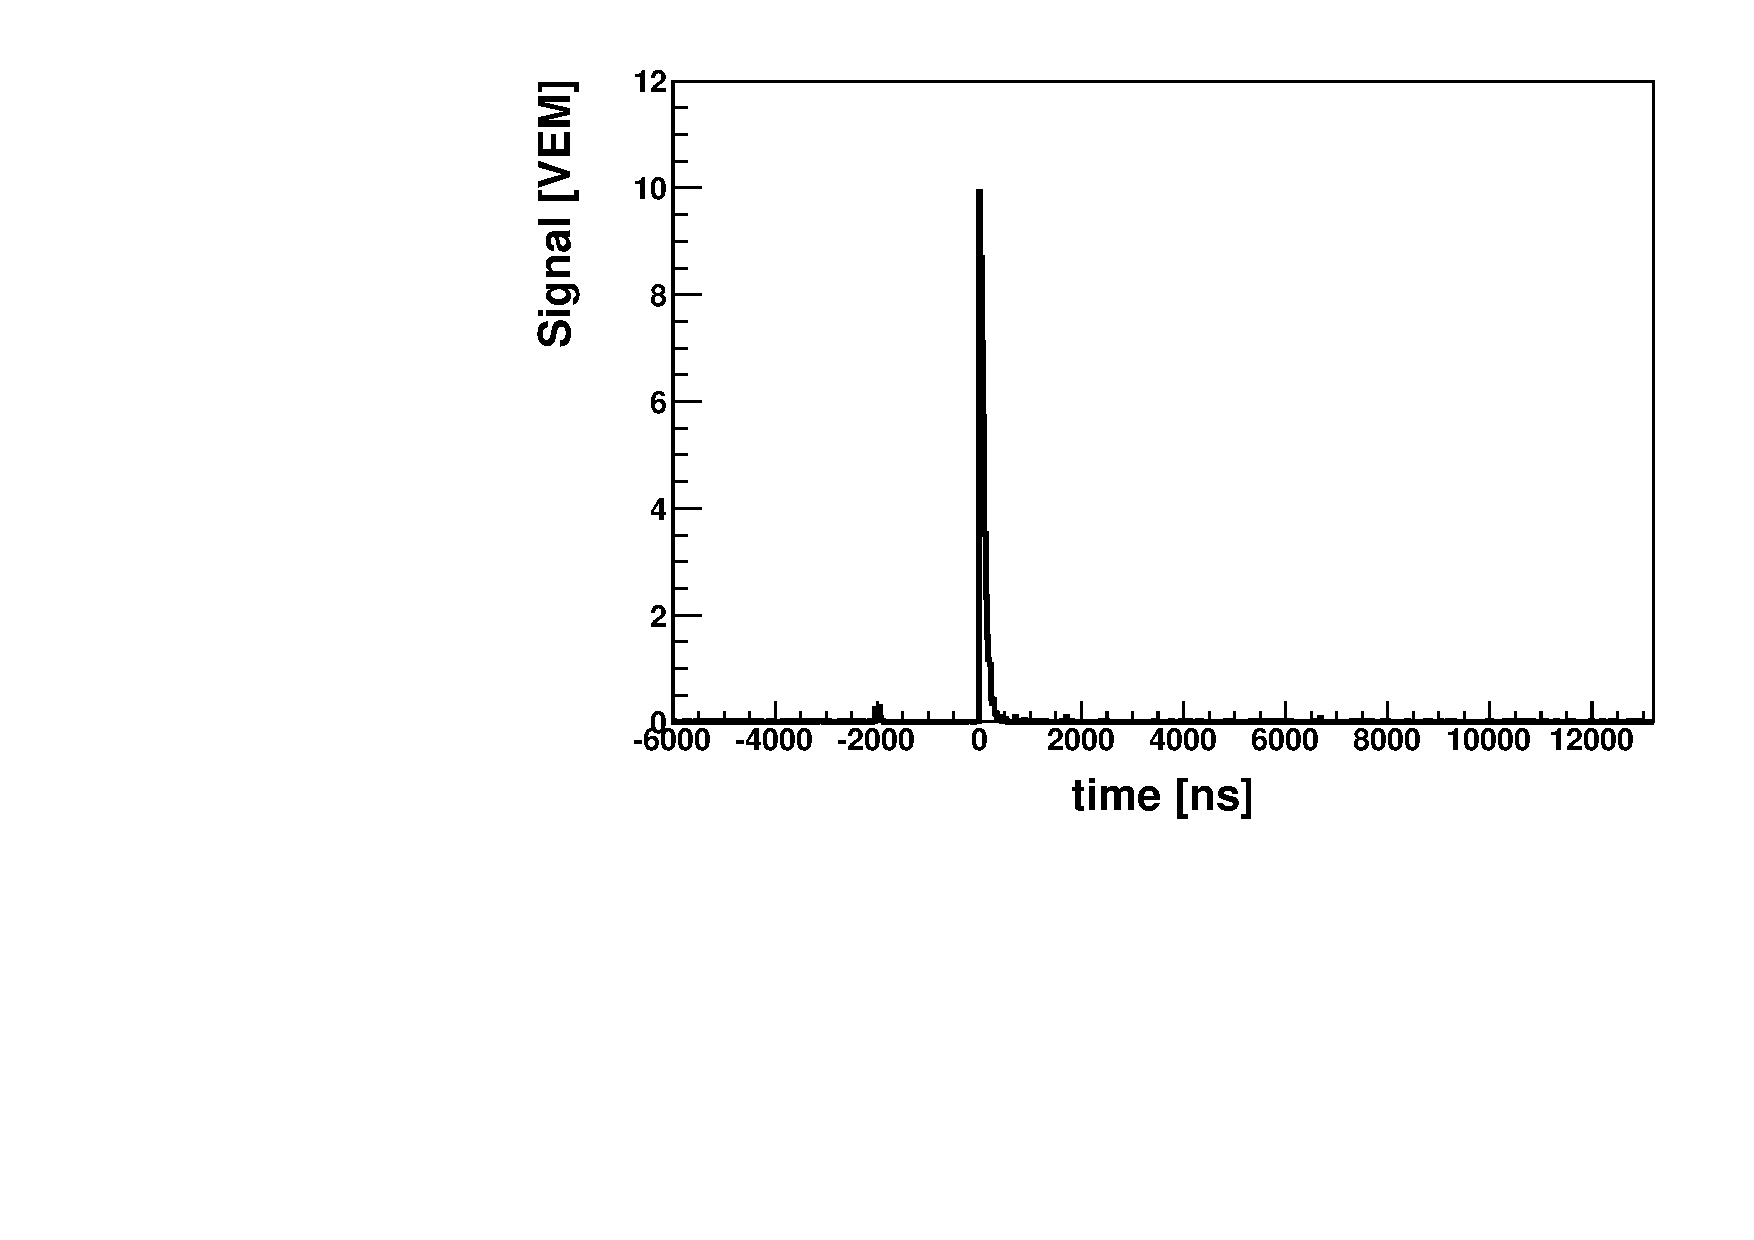
\includegraphics[width=0.6\textwidth]{fig/seleccionAuger/ev3995196_pmt1_anode.pdf}\\
			\includegraphics[width=0.6\textwidth]{fig/seleccionAuger/ev3995196_pmt2_anode_withEllipse.pdf}\\
			\includegraphics[width=0.6\textwidth]{fig/seleccionAuger/ev3995196_pmt3_anode.pdf}
			\end{array}
			$
			\vspace{-0.5cm}
			\caption{
			Ejemplo de un PMT descartado por permanecer como dudoso por un período largo de tiempo.
			Estación 1440 (Nirvana) para el evento 3995196 con fecha 28 de Septiembre de 2007.
			De arriba a abajo, PMT 1 a 3. El PMT número 2 se estiqueta como dudoso. La etiqueta se debe a la señal espúrea que se señala con una elípse sobre el final de la traza.
			}
			\label{fig:event3995196}
			\end{center}
		\end{figure}

	\subsection{Seleccion de estaciones}
	
	Hay varias rasones para descartar estaciones. Por ejemplo algunas de ellas poseen un solo PMT activo durante algún período de tiempo, o si cierto evento fue registrado durante una tormenta eléctrica, puede ser que la señal de radio emitida por un relámpago haya interferido con la electrónica, o simplemente algúm muon accidental disparó la estación que realmente no forma parte del evento.
	A continuación se detallan los procedimientos para descartar este tipo de anomalias.
	
		\subsubsection{Estaciones con un solo PMT activo}
		
		Aunque cada estación cuenta con 3 PMT's algunos pueden tener fallas temporales o permanentes, lo que hace necesario eliminarlos del análisis.
		Dado que la superficie instrumentada es inmensa e incluso a veces de dificil acceso, reemplazar o arreglar un PMT que presenta fallas puede llevar meses.
		Si un candidato a neutrinos apareciera, es necesario poder confirmar la señal en la estación por con al menos dos PTM's. 
		Si bien es raro, es posible que suceda que una estación siga funcionando con un PMT activo.
		En este caso, no sería posible realizar la confirmación de la traza, por lo que esa estación se descartaría del evento.
		
		\subsubsection{Estación con señales debidas a relámpagos}
		
		Una posible fuente de señales espúreas son los relámpagos.
		Cuando la señal electromagnética que generan alcanza la electrónica de adquisición de las estaciones, se registra una señal oscilante en el orden de los $\rm MHz$, como se observa en la figura \ref{fig:event1186354_st506_pmt}.
		%
		\begin{figure}[th!]
		\begin{center}
		\includegraphics[width=0.7\textwidth]{fig/seleccionAuger/event3995197_station506_pmt3.pdf}
		\caption{Ejemplo de una señal generada por un relámpago.
		La señal corresponde al PMT número 3 del evento 3995197 con fecha 26 de enero de 2005.}
		\label{fig:event1186354_st506_pmt3}
		\end{center}
		\end{figure}
		% 
		La oscilación en la señal se usa para detectar este tipo de sucesos.
		Si un evento contiene una estación de este tipo, se descarta.
		
		\subsubsection{Estaciones accidentales: efecto de los muones atmosféricos}
		
		El detector se encuentra expuesto a un flujo constante de muones atmosféricos mucho mas abundante que el de UHECR\footnote{Estos incluso se utilizan para el calibrado automático de las estaciones.}. 
		Al nivel del detector, \cant{1400}{m} sobre el nivel del mar, este se compone principalmente de muones en el rango de \cant{1-10}{GeV}. 
		Estas partículas, que no forman parte de los eventos que nos interesan, pueden afectar la reconstrucción de dos maneras:
		%
		\begin{enumerate}
		\item \textbf{Producir un trigger T2 en una estación de superficie que no pertenece al evento:} como las partículas que disparan la estación no pertenecen a la lluvia, el tiempo del T2 adicional tendrá una distribución uniforme en la ventana de 60~$\mu$seg del T3. Como la selección de lluvias inclinadas depende fuertemente de las posiciones y tiempos de disparo de las estaciones, una estación extra puede dar como resultado una incorrecta estimación de la geometría de la lluvia, especialmente en los eventos más pequeños.

		\item \textbf{Agregar señal espuria en alguna de las estaciones que sí pertenecen al evento:} si la señal accidental ocurre unos pocos $\mu$seg antes de que las partículas de la cascada atmosférica alcancen la estación, el resultado es que ambas señales se fusionan en una misma traza, siendo la señal espuria la que fija el tiempo de disparo del T2 producido (ver figura \ref{fig:trazaMalTiempo}). Esta modificación en el tiempo de disparo tiene efectos sobre la reconstrucción del evento. 
		Además del posible efecto sobre el tiempo de disparo, la señal espuria modifica los valores de los observables de la traza incluso si arriba unos $\mu$seg despúes que las partículas de la cascada. Como se discutirá más adelante, este efecto puede ser importante y será tenido en cuenta en la elaboración del criterio de identificación de neutrinos. 
		\end{enumerate}
		%
		\begin{figure}[ht]
		\begin{center}
		\includegraphics[width=0.75\textwidth]{fig/seleccionAuger/badStartTime.pdf}
		\caption{Efecto de un muón accidental en la determinación errónea del tiempo de disparo.}
		\label{fig:trazaMalTiempo}
		\end{center}
		\end{figure}
		
		Con el fin de minimizar el impacto de estas señales espúreas que producen los muones accidentales se aplica el siguiente procedimiento.
		
		\titulo{Algoritmo de limpieza de traza} la idea del método es simple, la cantidad de energía que los muones depositan en el tanque es, a primer orden, proporcional a la longitud del camino que recorren dentro del tanque.
		Dado que las estaciones son bastante más anchas que altas (\cant{1.2}{m} de alto por \cant{3.6}{m} de diametro), los muones inclinados producen una señal que, en promedio, es mayor que la producida por los verticales.
		
		Los muones accidentales son mayormente verticales como se puede ver figura \ref{fig:atmo_mu_flux}.
		Este hecho puede ser explotado para identificar qué fracción de la traza debe ser eliminada.
		%
		\begin{figure}[ht]
		\begin{center}
		\includegraphics[width=0.85\textwidth]{fig/seleccionAuger/atmo_mu_flux.pdf}
		\caption{Flujo de muones atmosféricos de acuerdo con la parametrización dada en~\cite{cite:atmo_mu}. Puede observarse que la mayoría presenta un ángulo cenital inferior a 50$^{\circ}$ ($\cos\theta \geqslant 0.6$)}.
		\label{fig:atmo_mu_flux}
		\end{center}
		\end{figure}
		
		El algoritmo de limpieza utilizado se describe en \cite{trace_cleaning}.
		Este comienza al nivel de cada PMT dentro del tanque:
		%
		\begin{enumerate}
		 \item Se extraen los segmentos de señal de cada PMT, definidos por al menos 2 bines consecutivos que presenten al menos 3 unidades de FADC por sobre la linea de base.
		 Se guardan los índices de inicio y fin, y se calcula la carga de cada segmento $Q$ y su pico $P$.
		 \item Se unen los segmentos si el gap entre ellos es de menos de 20 bines mas la longitud del primer segmento, y si al menso una de las siguientes condiciones se cumplen:
		 \begin{enumerate}
		  \item El primer segmento posee una señal $Q_1>0.3Q_2$
		  \item El segundo segmento posee de menos de 5 unidades FADC sobre la linea de base
		 \end{enumerate}
		El objetivo de estas condiciones es unir segmentos que hayan sido provocados por partículas de la lluvia.
		\item Se combinan las señales de los diferentes PMT's, combinando los segmentos que se superpongan mediante el promedio.
		\item El start time de los segmentos combinandos se toma de la contribución que posea la mayor señal.
		\end{enumerate}
		
		Como ejemplo, en la figure \ref{fig:atmo_mu_flux}, el algoritmo encuentra dos segmentos.
		En principio, el segmento con la señal integrada mas grande se conserva y el resto se descarta.
		Sin embargo, tambien podría ocurrir que uno o mas segmentos posean una señal similar, por lo que no sería claro cuál es el segmento que realmente interesa.
		Para salvar estas situaciones, se aplica un algoritmo especial, comenzando por segmentar la señal promedio con un criterio similar al que se aplica para segmentar la de los PMT's:
		%
		\begin{enumerate}
		 \item El segmento comienza con el primer bin que presente una señal por encima de los \cant{0.2}{VEM}.
		 \item En los siguientes 10 bines (\cant{250}{ns}) la carga integrada $Q$ debe superar los \cant{3}{VEM}. Si no, el inicio de la traza se muebe un bin hacia adelante hasta que las ambas condiciones se cumplan.
		 \item El final de la señal se define cuando a partir de él se encuentren 15 bines consecutivos por debajo de \cant{0.2}{VEM}.
		 \item Se calculan dos cantidades:
		 \begin{enumerate}
		  \item $nBoT$: el numero de bines por encima de \cant{0.2}{VEM}.
		  \item $Q_T$: la suma de la señal sobre los bines sobre \cant{0.2}{VEM}.
		 \end{enumerate}
		\end{enumerate}
		%
		A cada segmento se le asigna una puntuación $s=nBoT\times Q_T$. 
		Las trazas inducidas por muones atmosféricos tienden a tener valores de $s$ pequeños cuando se los compara con las inducidas por lluvias inclinadas.
		Si hubiera más de un segmento que cumpla $s>0.5s_{max}$, con $s_{max}$ la máxima puntuación, la estación es rechazada debido a que el tiempo de inicio de la señal es ambiguo.
		En caso contrario, el segmento con mayor puntuación se conserva y el resto se rechaza.
		La figura \ref{fig:multipicos} muestra un ejemplo de una estación que muestra tres segmentos similares. 
		%
		\begin{figure}[ht]
			\begin{center}
			\includegraphics[width=0.75\textwidth]{fig/seleccionAuger/multipicos.pdf}
			\caption{Traza que presenta múltiples segmentos de señal con características similares en la que no es posible determinar el tiempo de disparo T2. Los valores resaltados indican el puntaje asignado a cada segmento.}
			\label{fig:multipicos}
			\end{center}
		\end{figure}
		%
		Esta estación es removida del evento antes de aplicarle la reconstrucción.
		
	\subsection{Reconstrucción preeliminar}
	
	Una vez aplicados los precedimientos descriptos hasta el momento, los eventos cuentan con una lista de escaciones cuyos tiempos de disparo T2 se encuentran bien definidos.
	Sin embargo, los evetos todavia pueden contener estaciones disparadas por muones atmosféricos o incluso por una lluvias de baja energía.
	Con el fin de identificar las estaciones que realmente pertenecen al evento que nos interesa, se pide que las estaciones pertenecientes a los eventos satisfagan una serie de requerimentos de compacticidad espacial y temporal.
	
	\subsubsection{Eliminación de estaciones aisladas} 
	
	El primer paso es remover las estaciones aisladas pidiendo las siguientes dos condiciones:
	\begin{enumerate}
	 \item Criterio estandar: Se elimina una estación como aislada si no cuple que:
	 \begin{enumerate}
	  \item Existe una estación con T2 a menos de tres coronas, \cant{d_1=4700}{m}, y dentro de un rango temporal de compatible con un frente que se desplaza a la velocidad de la luz, \cant{t_1=\frac{d_1}{c}\sim15700}{ns}.
	  \item Eciste una segunda estación con T2 en la cuarta corona, \cant{d_1=6200}{m}, y con el mismo criterio temporal, \cant{t_2=\frac{d_2}{c}\sim20700}{ns}.
	 \end{enumerate}
	 \item Eliminación de señales muónicas: Si la magnitud de la traza es compatible con la señal de un muon vertical, ${\rm AoP} \equiv \frac{S}{S_{peak}}<1.4$, el criterio es mas estricto, pidiendo al menos una señal con T2 en la primer corona o en las estaciones cercanas de la segunda, \cant{d=2700}{m}.
	\end{enumerate}
	
	\subsubsection{Selección Top-Down} 
	
	El segundo paso consiste en la selección de estaciones compatibles con haber sido disparadas por el frente de partículas de una EAS.
	El algoritmo utilizado para este propósito se conoce como \emph{selección Top-Down} \cite{topDownSel}.
	
	La idea general del método consiste en ir descartando estaciones hasta encontrar una configuración que cumpla las condiciones requeridas.
	A continuación se expone el paso a paso del algorítmo:
	%
	\begin{enumerate}
	 \item Se realiza una reconstrucción del ángulo cenital del evento $\theta_{rec}$ asumiendo un frente plano y un tiempo de arrivo $t_0$, definido como el tiempo promedio de inicio de señales y pesado por las mimas. Este procedimiento se realiza analiticamente como se detalla en el apéndice \ref{ap:topDown}
	 \item Se evalua la compatibilidad temporal para cada estación y para el evento completo evaluando:
	 \begin{itemize}
	  \item $\Delta t_i < (N-2)\cdot 250{\rm ns} \cdot {\rm max}(\cos\theta_{rec},0.2)$
	  \item $\sum_i\Delta t_i^2 < \left[(N-2)\cdot 200{\rm ns} \cdot {\rm max}(\cos\theta_{rec},0.2)\right]^2$
	 \end{itemize}
	 donde $\Delta t_i$ es la diferencia entre el tiempo de T2 de la estacion $i$ y el obtenido mediante el ajuste del frente plano.
	 
	 Los cortes dependen de la multiplicidad del evento $N$ y de el ángulo reconstruido $\theta_{rec}$.
	 Debido a la curvatura del frente de la lluvia, las estaciones perisféricas presentan una mayor diferencia temporal respecto del frente plano que las centrales (ver figura \ref{fig:planeFrontAprox}). 
	 
	 La dependencia con el ángulo cenital aparece por una razón similar: las lluvias inclinadas llegan al detector tras atravesar mayor cantidad de materia que las verticales. Por este motivo, la dependencia del radio del frente de la lluvia se considera típicamente $R\propto\sec\theta$ \cite{cite:ShowerFront}, $R$ el radio de curvatura.
	 Consecuentemente, par ángulos cenitales grandes el frente de la lluvia presenta una curvatura pequeña ($R$ grande).
	 Para $\cos\theta < 0.2$, lo que corresponde a $\theta>80^\circ$, se asume que el mismo ha alcanzado su curvatura mínima.
	 Por esta razon, el mínimo tiempo de tolerancia para las estaciones respecto del frente plano será \cant{(N-2)50}{ns}.
	 \item Tambien se pide compacticidad espacial.
	 Todas las estaciones, proyectadas sobre el plano del frente de la lluvia, deben estar contenidas dentro de un círculo de radio $r_{max}$, con:
	 \begin{equation}
	  r_{max} = \sqrt{1300^2(N-2)}{\rm m}
	 \end{equation}
	 \item Se verifica la condición de T3.
	\end{enumerate}
	%
	\begin{figure}[ht]
	\begin{center}
	\includegraphics[width=0.85\textwidth]{fig/seleccionAuger/plano_vs_curvo.pdf}
	\caption{Esquema de la diferencia de tiempo entre un frente de lluvia curvo y su aproximación plana. 
	Las lluvias que generan alta multiplicidad de estaciones tienden a presentar diferencias de tiempo mayores al compararlas con la aproximación de frente plano.}
	\label{fig:planeFrontAprox}
	\end{center}
	\end{figure}
	%
	Si alguna de las condiciones no se satisface se intenta con las configuraciones de $N-1$ estaciones, quitando primero las de menor señal. 
	En cuanto todos los criterios se satisface, se acepta la configuración. Si no sucede, se quitan de a 2, 3 o hasta 4 estaciones.
	Si luego de probar todas las configuraciones quitando hasta 4 estaciones no se encontró ninguna configuración que satisfaga los criterios, el evento se descarta debido a la alta probabilidad de tener una mala reconstrucción.
	
	En el caso de que todas las estaciones de un evento sean alineadas, no es posible realizar la reconstrucción antes mencionada.
	En su lugar, se calcula la velocidad aparente de la señal $v_{ij}$ para cada par de estaciones $(i,j)$ con trigger T2:
	%
	\begin{equation}
	 V_{ij}=\frac{d_{ij}}{\Delta t_{ij}}
	\end{equation}
	%
	donde $d_{ij}$ es la distancia entre estaciones y $\Delta t_{ij}$ es la diferencia entre los tiempos de disparo.
	A partir de los valores de $V_{ij}$ se calcula la velocidad promedio $\langle V\rangle$ y la compatibilidad temporal se evalua para cada estación con la siguiente condición:
	%
	\begin{equation}
	 \frac{V_{ij}-\langle V\rangle}{\langle V\rangle}
	\end{equation}
	
	
	\subsection{Criterios adicionales}
	
	Una vez todas las estaciones con señales espúreas han sido descartadas, se evaluan algunos criterios de compacticidad adicionales que aseguran una mejor reconstrucción del core de la lluvia.
	
	\begin{enumerate}
	 \item \texttt{6T5}: es el criterio estandar del observatorio, que pide que la estación con mayor señal se encuentre rodeada por 6 estaciones activas. Sólo se aplica en la búsqueda de DGL.
	 \item \texttt{isConteined}: una vez reconstruido el core de la lluvia se identifica la estación con mayor señal y se requiere que se encuentre rodeada por 5 estaciones activas. Este criterio se utiliza en las búsquedas de DGH y ES. Esta condición es algo más laxa que el 6T5 en el sentido que permite que el core de la lluvia caiga algo más afuera del detector. Esto es posible para las búsquedas de DGH y ES dado que la contaminación debido al fondo es menos probable que para el rango angular que observa DGL.
	 \item \texttt{6T5 posterior}: igual que \texttt{isConteined} pero pidiendo que la estación se encuentre rodeada por 6 estaciones activas. Solo se aplica a DGL.
	 \item \texttt{hottestHasNeighbour}: este pide que la estación de mayor señal tenga en su primer corona otra estación con T2. El objetivo de este corte es evitar eventos de baja multiplicidad con ``agujeros''. Esta condición solo se requiere en el análisis de ES, donde los eventos reales que presentan este problema son raros pero aparecen.
	\end{enumerate}
	
\section{Selecci\'on de lluvias inclinadas}

Una vez generada la muestra de eventos de calidad, se encuentran dadas las condiciones para aplicar la selección de eventos inclinados.
Existen dos tipos de variables que permiten seleccionarlos:
\begin{enumerate}
 \item Directas: consisten en los distintos valores del parámetro $\theta$ obtenidos a partir de ajustar los tiempos de disparo de las estaciones con diferentes modelos de frente de onda (plano, cónico, esférico, parabólico, etc.)
 \item Indirectas: se refieren a otras variables sensibles a la inclinación, como por ejemplo la velocidad aparente de la señal o la elongación de la ``huella'' dejada por la lluvia sobre el detector.
\end{enumerate}
	
	\subsection{Reconstrucción angular}
	\label{sbsc:thetaRec}
	
	Para obtener un estimador del ángulo cenital se aplica un procedimiento iterativo.
	Como primer paso, sobre el conjunto de estaciones seleccionadas se realiza un ajuste asumiendo un frente plano.
	Este ajuste, más sofisticado que el que se realiza en la selección de estaciones, utiliza un modelo para la incerteza en el tiempo de disparo \cite{cite:ines}.
	Este modelo fue optimizado para describir lluvias horizontales hadrónicas iniciadas alto en la atmósfera en las que, por lo tanto, domina la componente muónica al nivel del detector (eventos inclinados típicos):
	%
	\begin{equation}
	\sigma_t = 20 \left[ 1 + \left( \frac{15}{S} \right)^{2/4.5} \right]
	\label{ec:varT} 
	\end{equation}
	%

% 	Es importante resaltar que, al utilizar este modelo, se elige priorizar la correcta reconstrucción de las lluvia hadrónicas (inmensa mayoría, si no la totalidad, de los datos) por sobre las posibles lluvias profundas iniciadas por neutrinos
% 	\footnote{Las lluvias profundas cuentan con una componente EM apreciable al alcanzar la tierra, lo que produce que la incerteza en su tiempo de disparo no sea correctamente descripta por el modelo anterior que asume que la cantidad de electrones y fotones es despreciable.}. 
	
% 	\textbf{CHARLAR SOBRE ESTO}
% 	Como se discutirá más adelante en la Sec.~\ref{sub:thetaRec}, esta elección produce una disminución en la eficiencia de detección de neutrinos pero se ve justificada ya que implica una disminución del fondo hadrónico debido a lluvias ``verticales'' ($\theta<75^\circ$) incorrectamente reconstruidas como ``horizontales'' ($\theta>75^\circ$).

	Una vez realizada la reconstrucción se evalúan las diferencias de tiempo $\Delta t_i$ entre las estaciones y el frente plano obtenido.
	Si alguno de los $\Delta t_i$ no está contenido en el intervalo [-300,700]~$\mbox{ns}$\footnote{
	Una vez producidos, los muones viajan sin desviarse y, en general, alcanzan la tierra antes que la componente EM. Las fluctuaciones en su tiempo de arribo son entonces menores a las esperadas para electrones y fotones que sufren multiples disperciones en su camino. Esta es la razón de que se tome un intervalo asimétrico.
	},
	la estación con mayor $\Delta t_i$ es removida y se repite la reconstrucción. Este procedimiento continua hasta que se encuentra una configuración aceptable.
	Si tras alguna de las iteraciones quedan menos de 4 estaciones el evento es rechazado.
	
	Si el evento está constituido por estaciones alineadas, el ángulo azimutal es fijado en la dirección de avance de la señal y se aplica el mismo procedimiento de reconstrucción antes mencionado.
	En el caso de eventos en linea el ángulo cenital obtenido es, en realidad, una cota mínima (ver Fig.~\ref{fig:conoLineEvent}).
	%
	\begin{figure}[ht]
	\begin{center}
	\includegraphics[width=0.75\textwidth]{fig/seleccionAuger/conoLineEvent.pdf}
	\caption{Esquema de reconstrucción geométrica de un evento en linea. Una cota mínima para el ángulo cenital se obtiene al considerar que el ángulo azimutal de la lluvia coincide con la linea que une las estaciones.}
	\label{fig:conoLineEvent}
	\end{center}
	\end{figure} 
	
	En la figura \ref{fig:resDGL} se muestra la resolución angular obtenida para lluvias DGL iniciadas por $\nu_e$ via CC, que se define como la desviación estandar de la diferencia entre el ángulo reconstruido y el simulado, $(\theta_{Rec}-\theta_{MC})$.
	%
	\begin{figure}[ht]
	\begin{center}
	\includegraphics[width=0.75\textwidth]{fig/seleccionAuger/resDGL.pdf}
	\caption{Resolución angular para lluvias DGL. En verde se resaltan los eventos iniciados alto en la atmósfera. Estos presentan una resolución debido a que el método de ajuste se encuentra optimizado para eventos hadrónicos.}
	\label{fig:resDGL}
	\end{center}
	\end{figure}
	%
	En verde se resaltan los eventos iniciados alto en la atmósfera (\cant{D<300}{g cm^{-2}}), que presentan una mejor resolución. 
	Esto se debe a que el método utilizado se encuentra optimizado para eventos hadrónicos, que se inician a una profundidad media de \cant{\sim100}{g cm^{-2}}.
	
	Dado que el problema esta mal condicionado para lluvias muy horizontales ($\sim90\deg$), no es posible utilizar este tipo de variables en el analisis de eventos ES.
	Para salvar este problema es necesario utilizar variables que no dependan de este tipo de ajuste, lo que se desarrolla en la sección \ref{sc:otrasVarIncl}.
	
	\subsubsection{Eventos espacialmente mal condicionados}
	\label{sub:illEvents}
	Definimos a un evento como ``espacialmente mal condicionado'' cuando está formado por un evento en linea más una estación no alineada. En otras palabras, es un evento no alineado que se vuelve en linea al remover una sola estación.
	Este configuración espacial es particularmente susceptible a producir una mala reconstrucción espacial. Para entender porqué, es útil considerar un caso límite: un evento totalmente vertical que dispara tres estaciones alineadas. En este caso, las tres estaciones tienen el mismo tiempo de T2 por lo que si se lo reconstruye como evento en linea se obtendría un ángulo cenital consistente con un evento vertical. Sin embargo, en el caso de que junto con el evento ocurriera el disparo de una estación accidental no alineada, el evento se reconstruiría como no alineado y el ángulo cenital sería determinado sólo por el tiempo de la estación extra. En resumen, una sola estación sería la que determinaría la geometría reconstruida del evento.

	Para evitar este problema, los eventos que presentan una configuración espacial mal condicionada se someten a una selección adicional. 
	Se ignora la estación no alineada, se reconstruye el evento en línea resultante y se exige que éste también sea inclinado.
	
	
	\subsection{Otras variables sensibles a la inclinación}
	\label{sc:otrasVarIncl}
	
	
	Además de obtener una estimación directa del ángulo cenital $\theta$ a partir de un ajuste, es posible utilizar otro tipo de variables sensibles a la inclinación, como la velocidad aparente de la señal o la elongación de la huella sobre el detector.
	Mediante este tipo de variables es posible salvar las situaciones en las que la reconstrucción angular no puede ser llevada a cabo.
	Esta situación sucede muy frecuentemente para los neutrinos DGH casi horizontales y casi para la totalidad de los neutrinos ES.
	
		\subsubsection{Huella del evento}
		Los eventos inclinados tienden a producir una huella de señal elongada sobre el SD.
		Con el fin de cuantificar esta característica se construye un ``tensor de señal'':
		%
		\begin{eqnarray}
		S = \sum_i s_i, \quad \langle X \rangle = \sum_i s_i x_i/S, \quad \langle Y \rangle = \sum_i s_i y_i/S \nonumber \\
		I_{xx} = \sum_i s_i (x_i - \langle X \rangle)^2 / S, \quad I_{yy} = \sum_i s_i (y_i - \langle Y \rangle)^2 / S \nonumber \\
		I_{xy} = I_{yx} = \sum_i s_i (x_i - \langle X \rangle)(y_i - \langle Y \rangle) / S 
		\end{eqnarray}
		%
		Este objeto describe la distribución espacial de señal de misma forma en que el tensor de inercia, aplicado a un objeto extenso, lo hace con la masa.
		Continuando con esta analogía (ver figura \ref{fig:elipse}) se pueden obtener los ejes de la elipse de señal como:
		%
		\begin{eqnarray}
		L^2 =\frac{I_{xx}+I_{yy}+\sqrt{(I_{xx}-I_{yy})^2 + I_{xy}^2 }}{2S} \nonumber\\
		W^2 =\frac{I_{xx}+I_{yy}-\sqrt{(I_{xx}-I_{yy})^2 + I_{xy}^2 }}{2S} 
		\end{eqnarray}
		%
		Siendo $L$ la longitud del semieje mayor y $W$ la del menor (ver figura \ref{fig:elipse}).

		Como se discute en la sección \ref{sbsc:thetaRec}, es posible que una lluvia vertical junto con una estación accidental den como resultado un ángulo cenital reconstruido compatible con una cascada inclinada.
		Sin embargo, estos eventos no suelen presentar una huella elongada.
		De esta manera, el cociente $L/W$ puede usarse como criterio de calidad para eventos inclinados.
		
		\subsubsection{Velocidad aparente de la señal}
		En un evento inclinado genuino, el eje de la lluvia coincide con la dirección del semieje mayor de la elipse.
		Así, la velocidad aparente de la señal $V$ en ésta dirección permite obtener una buena aproximación del ángulo cenital.
		%
		\begin{equation}
		\sin\theta \simeq \frac{V}{c}
		\end{equation}
		%
		Para estimar $V$ a partir de un evento, se promedian las velocidades $V_{ij}\equiv L_{ij}/\Delta T_{ij}$ entre pares de estaciones cuya distancia, proyectada en la dirección del semieje mayor, sea superior a los \cant{1000}{mts} (ver panel derecho en la figura \ref{fig:elipse}).
		No se consideran los pares de estaciones con distancia $L_{ij}$ pequeñas ya que, producto de la propagación de la incerteza en el tiempo de disparo, presentan un error inaceptable en la velocidad de la señal estimada.
		%
		\begin{figure}[ht]
		\begin{center}
		\includegraphics[width=1.0\textwidth]{fig/seleccionAuger/elipse.pdf}
		\caption{Diagrama de la elipse de señal que describe la configuración espacial de un evento inclinado (izquierda). Representación del cálculo de la velocidad de la señal en la dirección del semieje mayor (derecha).}
		\label{fig:elipse}
		\end{center}
		\end{figure}
		%
		
		\subsection{Eventos de 3 estaciones en ES}
		\label{sbsc:3StIncl}
		
		Los eventos de 3 estaciones son problemáticos debido a que es usual que presenten gran incerteza en su reconstrucción. 
		Por ende, tienen alta probabilidad de ser clasificados como inclinados cuando no lo son, tanto es así, que en las búsquedas de DG no son utilizados.
		En cambio, en la búsqueda de ES no pueden descartarse ya que representan al rededor del 30$\%$ de la muestra de señal. 
		Por este motivo para incluirlos se debe tener especial cuidado en su selección, cuando se los clasifica como inclinados y como jóvenes.
		
		Hay sólo 7 configuraciones de tres estaciones que  satisfacen los requisitos de trigger T3, que se muestran en la figura \ref{fig:3stConf}.
		Gracias a que este número es manejable, además de aplicarles cortes en las variables presentadas hasta el momento, se pedirá un requisito adicional sobre la configuración.
		La idea es conservar las configuraciones propensas a aparecer en la muestra de señal mientras se eliminan las que proclives a inducir candidatos falsos.
		%
		\begin{figure}[ht!]
		\begin{center}
		\includegraphics[width=1.0\textwidth]{fig/seleccionAuger/3stConf}
		\caption{Bosquejo de las 7 posibles configuraciones de 3 estaciones que pueden lograr disparo T3. Cabe destacar que cada estación debe haber disparado con nivel ToT.}
		\label{fig:3stConf}
		\end{center}
		\end{figure}
		%
		En la tabla \ref{tab:3stConf} muestra la frecuencia de aparición en el MC de neutrinos ES luego de aplicar los criterios de calidad.
		%
		\begin{table}[!h]
		\centering
		\begin{tabular}{|c|c|c|c|c|}
		\hline
		Config. & MC Events & Porent. & Porcent Pesado & Datos                  \\
		\hline
		Total & 3562 & 100\% & 100\%& 10329\\
		\hline
		1 & 1993 & 56.0\% & 70.8\% & 1378\\
		2 & 132 & 3.7\% & 0.5\% & 1895\\
		3 & 3 & $<$0.1\% & $<$0.1\% & 6358\\
		4 & 142 & 4.0\% & 1.8\% & 82\\
		5 & 1278 & 35.9\% & 26.9\% & 378\\
		6 & 8 & 0.2\% & $<$0.1\% & 38\\
		7 & 9 & 0.2\% & $<$0.1\% & 200\\
		\hline
		\end{tabular}
		\caption{
		\label{tab:3stConf}
		Frecuencia de aparición de las distintas configuraciones mostradas en la figura \ref{fig:3stConf} luego de aplicar los criterios de calidad.
		Se muestran, de la columna 2 a 4 la cantidad de eventos MC en cada donfiguración, porcentage de aparición y su porcentaje pesado.
		La última columna muestra el número de eventos en la muestra de fondo que presentan cada configuración.
		}
		\end{table}
		%
		En la muestra de señal, compuesta por eventos muy inclinados, las dos configuraciones dominntes son la 1 y la 5. Las razones por las que el resto de configuraciones no son frecuentes son las siguientes:
		\begin{itemize}
		 \item Las configuraciones 2 y 3 son demasiado compactas y anchas. Los neutrinos ES típicamente dejan huellas muy alargadas. Si un evento ES tuviera el ancho suficiente para disparar esas tres estaciones, usualmente dispararía algunas más, generando un evento de mayor multiplicidad.
		 \item Las configuraciones 6 y 7 son improbables dado que en el caso de haber una estacion dentro del triángulo formado por las tres estaciones disparadas, tambien sería disparada.
		 \item La configuración 4 es la tercera en abundancia. Esto es rasonable debido a que es una configuración bastante alineada, típica de neutrinos ES. Sin embargo, se encuentra desfavorecida debido a que requiere una estación intermedia no disparada.
		\end{itemize}
		
		Claramente, desde el punto de vista de mantener alta eficiencia a neutrinos ES, no se gana mucho conservando las configuraciones 2, 3, 4, 6 y 7, por lo que, siendo conservador, son descartadas.
		En cambio, la configuración 1 además de ser frecuente, es compacta, por lo que sin dudas deberá ser conservada.
		Por otro lado, dado que hasta el momento Auger no ha detectado ningun neutrino, se consideró que un candidato a neutrino que presente la configuración 5 daría lugar a escepticismo departe de la comunidad. Por todo esto, en la búsqueda de neutrinos ES, sólo se aceptan eventos de 3 estaciones de configuración 1.
		
		\subsection{Desempeño de la selección de eventos inclinados}
		
		La selección de eventos inclinados se realiza en cada análisis utilizando los cortes que aparecen en la tabla \ref{tab:inclSel}.
		Estos cortes fueron definidos en base a un compromiso entre conseguir alta eficiencia de selección de eventos iniciados por neutrinos y evitar la aceptación de datos poco inclinados que posean alta componente electromagnética.
		%
		\begin{table}[ht!]
		\begin{center}
			\renewcommand{\arraystretch}{1.4}
			\scriptsize
			\begin{tabular}{|l|c|c|c|}
			\hline
			Búsqueda & Earth-skimming (ES)           & Downward-going                        & Downward-going                       \\
					&                               & {\it high} angle (DGH)                & {\it low} angle (DGL)                \\
			\hline
						& $-$                             & $\theta_{\rm rec}>$ 75$^{\circ}$   &   $\theta_{\rm rec}\in (58.5^\circ,~76.5^{\circ})$\\
			Lluvias    & $L/W > 5$                                         & $L/W > 3$ & $-$ \\
			Inclinadas & $\langle V\rangle\in (0.29,~0.31)~{\rm m~ns^{-1}}$ & $\langle V \rangle~<~0.313~{\rm m~ns^{-1}}$ & $-$ \\
					& RMS($V$)$~<~0.08~{\rm m~ns^{-1}}$                 & RMS($V$)/$\langle V\rangle<0.08$ & $-$ \\
					& Conf 1 si $N_{ST}=3$ & & \\
			\hline
			Efficiencia & \multicolumn{3}{c|}{$\sim90\%$}\\
			\hline
			\end{tabular}
			\vskip -3mm
			\caption{Resumen de los observables y valores numéricos de los cortes aplicados para seleccionar lluvias inclinadas en las tres búsquedas de neutrinos.} 
		\end{center}

		\label{tab:inclSel}
		\end{table}
		%
		Dado que la muestra de fondo consiste en una fracción de los datos del detector, también se tuvo en cuenta que esta selección admita una cantidad suficiente de eventos que luego serán necesarios para definir el criterio de selección de lluvias jóvenes.
		
		En los tres análisis la eficiencia de selección para la muestra de señal representó al rededor del $\sim90\%$ de los eventos, pesados según lo que se expuso en la sección \ref{sc:pesos}.
		
\section{Selecci\'on de lluvias j\'ovenes}
	
	Una vez aplicadas a las muestras de fondo y señal las selecciones de eventos de calidad y de lluvias inclinadas, se definió la selección de lluvias jóvenes mediante el método iterativo que se esquematiza en la figura \ref{fig:entrenamiento}.
	%
	\begin{figure}[ht!]
		\begin{center}
		\includegraphics[width=1.0\textwidth]{fig/seleccionAuger/entrenamiento}
		\caption{Diagrama de flujo del método utilizado para definir la selección de lluvias jóvens en los tres análisis.}
		\label{fig:entrenamiento}
		\end{center}
	\end{figure}
	%
	Este método tiene tres pasos claramente definidos:
	\begin{enumerate}
	 \item \textbf{Definición de variables discriminantes}: consiste en definir mediante argumentos físicos variables que contengan información\footnote{en el sentido estadístico de la palabra} sobre si un evento pertenece a la muestra de señal o a la muestra de fondo.
	 \item \textbf{Entrenamiento del método}: en esta etapa se extrae la información de las variables para definir un posible criterio de selección. 
	 \item \textbf{Estimación de la eficiencia y la contaminación}: se evalua el criterio preeliminar definido en el punto anterior. Si la separación entre muestras es lo suficientemente buena, y la probabilidad de obtener eventos espúreos debidos al fondo es aceptable se aprueba el método. Caso contrario se vuelve al paso 1 y se modifica el conjunto de variables discriminantes.
	\end{enumerate}
	%
	\subsection{Variables discriminantes}
	\label{sbsc:discVars}
	
	En el capitulo \ref{sc:easNu} se argumentó que las lluvias hadrónicas inclinadas se inician muy alto en la atmósfera y sólo su componente muónica alcanza el detector.
	En cambio, las iniciadas por neutrinos tienen la posibilidad de interactuar de manera profund, presentando una cantidad significativa de componente electromagnética (EM) a la hora de interactuar.
	En el caso de los eventos DG, la componente EM se consentra en la región del detector sobre la que la lluvia interactúa primero, llamada zona temprana del evento.
	Por otro lado, los eventos iniciados por neutrinos ES, al desplazarse hacia arriba en la atmósfera, tienen la posibilidad de producir señal del tipo EM en todas las estaciones del evento.
	Esto se ilustra en la figura \ref{fig:compNus} en la que se representan las componentes muónica y electromagnética de una lluvia hadrónica típica, de un neutrino DG y de uno ES.
	%
	\begin{figure}[ht!]
		\begin{center}
		\includegraphics[width=0.7\textwidth]{fig/seleccionAuger/inclined_regular_dg_and_up}
		\caption{Arriba: Esquema de una lluvia inclinada iniciada por un hadrón que interactúa alto en la atmósfera. Medio: Lluvia profunda iniciada por un neutrino DG. La parte temprana del evento presenta una señal electromagnética significativa. Abajo: evento iniciado por un \tauon{} que emerge de la tierra producto de un neutrino ES. La componente electromagnética puede alcanzar todas sus estaciones.}
		\label{fig:compNus}
		\end{center}
	\end{figure}
	%
	
	En consecuencia, el objetivo es conseguir variables del detector que sean sensibles a la precencia de componente electromagnética.
	Esta, usualmente provoca señales en el SD cuya duración puede alcanzar algunos cientos de nano segundos, mientras que las señales generadas por la componente muónica no suele superar la centena.
	Entonces, a partir de las trazas FADC es posible construir observables correlacionados con la estructura temporal de la señal y analizar su desempeño.
	A continuación se definen algunos de los posibles observables:
	\begin{itemize}
	 \item \textbf{Numero de estaciones con trigger ToT:} como se discutió en la sección \ref{sbsc:trig_levels}, el triger ToT fue ideado para detectar señales extendidas en el tiempo.
	 Por ello, un observable sensible a la señal electromagnética en un dado evento podría ser la cantidad de estaciones con este nivel de trigger.
	 El problema con esta variable es que, al ser discreta dificulta cualquér estimación de fondo.
	 \item \textbf{RT/FT:} Se llama Rise Time (RT) y Fall Time (FT) al tiempo que le toma a la señal alcanzar desde el $10\%$ de su integral hasta el $50\%$ y desde el $50\%$ hasta el $90\%$ respectivamente.
	 Estas poseen al ventaja de que son una medida directa del observable que nos interesa, la duración de la señal, por lo que ambas variables muestran poder de discriminación entre la muestra de señal y de fondo (ver figura \ref{fig:diretObs}).
	 Por otro lado, la precencia de \emph{outliers} en la muestra de fondo dificulta el control de la contaminación.
	 Este tipo de señales, aunque poco frecuentes, son inaceptables en una busqueda de señal esperada tan pequeña como es la de neutrinos.
	 %
	 \begin{figure}[ht!]
		\begin{center}
		\includegraphics[width=0.48\textwidth]{fig/seleccionAuger/rt1}
		\hfill
		\includegraphics[width=0.48\textwidth]{fig/seleccionAuger/ft1}
		\\
		\includegraphics[width=0.48\textwidth]{fig/seleccionAuger/rt_forThesis}
		\hfill
		\includegraphics[width=0.48\textwidth]{fig/seleccionAuger/ft_forThesis}
		\caption{Distribuciones de $\log RT$ y $\log FT$, arriba para eventos DGH y abajo para eventos ES. Si bien en ambos casos se evidencia separación entre las muestras, la aparición de \emph{outliers} dificulta el control de la contaminación debido al fondo.}
		\label{fig:compNus}
		\end{center}
	\end{figure}
	 %
	 \item \textbf{AoP:} se llama AoP, o Area Over Peak, a la la integral de la FADC (su área) dividida por el máximo valor que haya alcanzado, como se muestra en la figura \ref{fig:aopDef}.
	 %
	 \begin{figure}[ht!]
		\begin{center}
		\includegraphics[width=0.6\textwidth]{fig/seleccionAuger/AoP_def}
		\caption{Definición de la variable AoP. Esta consiste en la integral de la FADC dividida por el máximo valor que esta haya alcanzado. Esta variable toma valores cercanos a uno para señales muónicas y mayores para electromagnéticas.}
		\label{fig:aopDef}
		\end{center}
	 \end{figure}
	 %
	 Esta variable se calibra para que los muones verticales tengan un valor medio de AoP$=1$.
	 En cambio, las señales cuyo origen es la componente EM de la lluvia presentan valores mucho mayores, como se observa en la figura \ref{fig:aopDist}.
	 %
	 \begin{figure}[ht!]
		\begin{center}
		\includegraphics[width=0.6\textwidth]{fig/seleccionAuger/aopDGL} \\
		\includegraphics[width=0.6\textwidth]{fig/seleccionAuger/aop_forThesis}
		\caption{Distribuciones de la variable AoP para señál y fondo. Arriba para neutrinos DGL y abajo para eventos ES. En ambos casos los eventos inclinados de la muestra de fondo presentan valores cercanos a 1 mientras que el valor medio para las muetras de señal es mayor.}
		\label{fig:aopDist}
		\end{center}
	 \end{figure}
	 %
	 Además de buena separación, esta variable no presenta colas largas en la muestra de fondo, por lo que el control de la contaminación se ve favorecido.
	\end{itemize}
	
	Las variables definidas hasta el momento se calculan de manera local, es decir, para cada estación.
	Para extraer la mayor cantidad de información posible, es necesario utilizar variables globales, que además de la información local, incluyan correlaciones entre las variables en distintas estaciones.
	A continuación se detallan las variables estudiadas en los distintos análisis.
	
	\subsubsection{ToTF}
	La variable \emph{ToT fraction} ToTF se define como la fracción de estaciones del evento que dispararon con trigger ToT y además poseen un valor de AoP$\geq1.4$.
	La distribución de esta variable se muestra en la figura \ref{fig:totfDist}.
	%
	\begin{figure}[ht!]
		\begin{center}
		\includegraphics[width=0.6\textwidth]{fig/seleccionAuger/ToTF_forThesis}
		\caption{Distribuciones de la variable ToTF para señal y fondo. Si bien la separación exhibida entre las muestras es notable, la posibilidad de estimación de la contaminación se ve desfavorecida.}
		\label{fig:totfDist}
		\end{center}
	\end{figure}
	%
	Si bien la separación exhibida entre las muestras es notable, la posibilidad de estimación de la contaminación se vuelve extremadamente dificil.
	
	\subsubsection{Variables derivadas de AoP}
	
	Para analizar la evolución de la variable AoP a lo largo del evento, resulta útil observar su promedio según el órden de disparo de las estaciones dentro del evento, lo que se grafica en la figura \ref{fig:aop_vs_NStation} para eventos de seis estaciones.
	%
	\begin{figure}[ht!]
		\begin{center}
		\includegraphics[width=0.8\textwidth]{fig/seleccionAuger/aop_vs_NStation}
		\caption{Promedio de AoP en función del número de la estación. Este se asigna según el órden de disparo dentro de cada evento. Se observa que los eventos DG presentan mayor diferencia en las estaciones tempranas, mientras que en los eventos ES esta se mantiene a lo largo de todo el evento.}
		\label{fig:aop_vs_NStation}
		\end{center}
	\end{figure}
	%
	De esta se deduce claramente que los eventos DG presentan mayor separación en las estaciones más tempranas de los eventos, mientras que en las lluvias ES esta se mantiene a lo largo de todos los tanques.
	Este comportamiento se mantiene para eventos de todas las multiplicidades.
	
	Teniendo esto en cuenta, se consideraron tres tipos de variables:
	\begin{enumerate}
	 \item \textbf{Producto de AoPs:} por las razones ya expuestas, se espera que las lluvias inclinadas presenten valores de AoP elevados. Así, su producto es una medida de esta característica global del evento. Una de las ventajas de esta variable discriminante es que es muy estable frente a fluctuaciones que puedan sufrir las estaciones individuales (ver panel superior izquierdo en la figura \ref{fig:observablesGlobales}). 
	 \item \textbf{Promedio de AoPs:} del mismo modo, el AoP promediado sobre todas las estaciones es otra variable prometedora que posee las mismas bondades que la anterior (ver panel superior derecho en la figura \ref{fig:observablesGlobales}).
	 \item \textbf{Asimetría:} en el caso de las lluvias DG, la diferencia entre las AoPs promediadas sobre las primeras  y las últimas estaciones de un evento puede ser otra variable con poder discriminante (ver panel inferior en la figura \ref{fig:observablesGlobales}). 
	\end{enumerate}
	%
	\begin{figure}
	\begin{center}
	\includegraphics[width=0.47\textwidth]{fig/seleccionAuger/aop_prod.pdf} \hfill
	\includegraphics[width=0.47\textwidth]{fig/seleccionAuger/trainning_withMCSimple_log_forThesis}\\
	\includegraphics[width=0.47\textwidth]{fig/seleccionAuger/asim.pdf}
	
	\caption{Distribución de la asimetría del AoP promedio entre estaciones tempranas y tardias (izquierda arriba) y producto del AoP en las cuatro estaciones más tempranas (derecha).}
	\label{fig:observablesGlobales}
	\end{center}
	\end{figure}
	%
% 	\clearpage
	\subsection{Entrenamiento del método}
	
	Una vez definidas las posibles variables discriminantes, es necesario optimizar su conjunto, ejecutando lo que se denomina entrenamiento del método.
	
	La opción más sencilla es aplicar lo que se denominan \emph{cortes cuadrados duros}.
	Este, es un método que consiste en definir una sucesión de variables y fijar sobre ellas cortes que permitan selecciónar a cada paso una fracción (en principio alta) de la muestra de señal.
	La ventaja principal de este método es que es relativamente simple, ya que el conjunto de variables elejidas y cada corte puede comprenderse usualmente mediante argumentos físicos.
	Por otro lado, su principal desventaja es que desperdicia cualquier información guardada en la correlación de las variables.
	
	Para subsanar este inconveniente, es común recurrir a lo que se denominan métodos multivariados o MVA por sus siglas en inglés.
	Estos poseen la ventaja de combinar la mayor parte de la información disponible y obtener así el mayor grado de separación posible, usualmente a costa de esconder la interpretación física del problema.
	Existen en la actualidad una gran variedad de herramientas de este tipo. Entre las más comunmente utilizadas se encuentran: redes neuronales, arboles de decisión y el análisis de componentes principales. 
	Con el objetivo de mantener una interpretación física simple, se en las b´usquedas de neutrinos de Auger se decidió adoptar el método de Fisher~\cite{cite:Fisher} para la construcción del algoritmo de identificación.

	La técnica de Fisher forma parte de los métodos de discriminación lineales.
	Partiendo de un conjunto de variables discriminantes construye un nuevo observable ${\cal F}$ como una combinación lineal de ellas.
	Este discriminante es óptimo para el caso de variables gaussianas y, en el caso general, provee la función lineal que brida la mayor separación posible.
	Además, al ser ${\cal F}$ suma de variables aleatoreas, su distribución tiende a ser más gaussiana que la de las variables originales.
	En la Fig.~\ref{fig:ideaFisher} se muestra la idea de funcionamiento del método en un caso particular idealizado.
	%
	\begin{figure}[ht]
	\begin{center}
	\includegraphics[width=0.75\textwidth]{fig/seleccionAuger/ideaFisher}
	\caption{Esquema de la idea de funcionamiento del método de Fisher. Ninguna de las dos variables originales es capaz de separar las muestras (cuadrados azules y circulos rojos) por si solas. Sin embargo una combinación lineal de ellas logra en este caso una separación completa. El método de Fisher permite obtener las constantes de la combinación lineal óptima (ver texto) a partir de las variables discriminantes provistas.}
	\label{fig:ideaFisher}
	\end{center}
	\end{figure}
	%

	Se define el discriminante de Fisher ${\cal F}$ como:
	%
	\begin{equation}
	{\cal F} = a_1 x_1 + .. + a_n x_n = \vec{a}\cdot \vec{x}
	\end{equation}
	%
	en donde $\vec{a}$ es el vector de los coeficientes de Fisher y $\vec{x}$ un vector que contiene las variables originales.
	Así, puede calcularse la media y la varianza del discriminante usando:
	%
	\begin{eqnarray}
	\langle{\cal F}_X\rangle &=& \vec{a}\cdot\vec{\mu}_X \\
	\text{Var}({\cal F}_X)   &=& \vec{a}^{\,T} \cdot \text{Cov}(X) \cdot\vec{a}
	\end{eqnarray}
	%
	siendo $\vec{\mu}_X$ el vector de valores medios de las variables de la muestra $X$ y Cov$(X)$ su matriz de covarianza.

	A partir de estos ingredientes se construye la función $Q(\vec{a})$ que cuantifica la separación provista por el discriminante $\cal{F}$
	entre las muestras señal y background a la vez que pondera su dispersión:
	%
	\begin{equation}
	Q(\vec{a}) = \frac{( \langle{\cal F}_S\rangle - \langle{\cal F}_B \rangle)^2}{\text{Var}({\cal F}_S)+\text{Var}({\cal F}_B)}
	= \frac{(\vec{a}\cdot\vec{\mu}_S  - \vec{a}\cdot\vec{\mu}_B)^2}
					{\vec{a}^{\,T} \cdot (\text{Cov}(S) + \text{Cov}(B) )\cdot\vec{a}} 
	\end{equation}
	%
	en donde ${\cal F}_S$ y ${\cal F}_B$ representan los valores del discriminante de Fisher para las muestras de señal y fondo respectivamente.
	Al maximizar esta función respecto de los coeficientes $\vec{a}$, se obtiene la combinación lineal de variables que optimiza la separación entre los grupos señal y background a la vez que minimiza sus varianzas manteniendo las distribuciones compactas para evitar la superposición. 
	Estos coeficientes $\vec{a}_{\text{Max}}$ están dados por:
	%
	\begin{equation}
	\vec{a}_{\text{Max}} = (\text{Cov}(S) + \text{Cov}(B) )^{-1} \cdot (\vec{\mu}_S - \vec{\mu}_B)   
	\end{equation}
	
	
	\subsection{Criterio de identificación - Estimación de fondo}
	\label{sbsc:fondo}
	
	Una vez construido el discriminante ${\cal F}$ o definido el conjunto de variables sobre las que se aplican los cortes cuadrados, es posible definir el valor de corte entre eventos hadrónicos y aquellos iniciados por neutrinos.
	Debido a que la señal de neutrinos que se intenta medir es muy pequeña, la sensibilidad del análisis está básicamente limitada por la magnitud de la contaminación esperada.
	Por esto, es fundamental lograr una estimación de la misma y a partir de ella fijar los cortes de selección de manera tal que sea lo suficientemente pequeña.
	
	Una forma de posicionar el corte es de manera tal que se esperen menos de un evento de fondo cada una cierta cantidad de años $N_{yr}$.
	Para ello, es necesario diseñar un modelo que permita obtener una extrapolación de la cantidad de eventos esperados para el período deseado.
	La estrategia adoptada en los tres análisis fue modelar la cola de la distribución de la muestra de fondo, que corresponde a una cantidad de años de datos del detector y renormalizarla a los $N_{yr}$ años (ver  figura\ref{fig:estimaBackground}) para poder calcular la posición del corte.
	%
	\begin{figure}[ht]
	\begin{center}
	\includegraphics[width=0.8\textwidth]{fig/seleccionAuger/estimaBackground.pdf}
	\caption{Estimación de background debido a eventos hadrónicos que puedan ser erróneamente clasificados como candidatos a neutrinos.}
	\label{fig:estimaBackground}
	\end{center}
	\end{figure}
	%
	
	En este marco, es interesante discutir que el teorema central del límite indica que el discriminante de Fisher, por ser la suma de variables aleatorias, tiende a una distribución gausiana al aumentar el número de términos.
	Sin embargo, debido a que como se verá en las siguientes secciones, la cantidad de variables utilizadas es bajo y además cada una de estas presenta distribuciones asimétricas, no es posible alcanzar un comportamiento gausiano.
	Por ende, para modelar la cola de las distribuciones fue necesario generar proponer un comportamiento motivado por las características físicas propias del sistema que se analiza.
	
	Debido a que la profundidad de interacción de las lluvias iniciadas por hadrones sigue una distribución exponencial, es esperable que esta característica se vea reflejada de alguna manera en la distribución de las variables discriminantes asociadas a las lluvias más profundas.
	Bajo esta hipótesis en los tres análisis es posible realizar un ajuste exponencial sobre la cola de las distribuciones de fondo en la región $[1\sigma, 3\sigma]$ (con esta notación denominamos al intervalo $[\mu+1\sigma, \mu+3\sigma]$, donde $\mu$ y $\sigma$ son la media y el RMS de la distribución de fondo) y extrapolar el comportamiento.
	Luego, con el fin de evaluar la bondad del ajuste, es posible utilizar las regiones de $[3\sigma, 4\sigma]$, $[4\sigma, 5\sigma]$ y $[5\sigma, 6\sigma]$, calculando en cada una la cantidad de eventos predichos por el ajuste con lo observado.
	Si los resultados son compatibles se renormaliza la distribución a $N_{yr}$ y se coloca el corte tal que se espere un evento por encima del mismo. Con el corte definido se evalua la eficiencia de selección de neutrinos. Si se obtiene un buen nivel de predicción en las zonas de $[3\sigma, 6\sigma]$ y el nivel de eficiencia es aceptable, se acepta el criterio de selección. En caso contrario, se debe realizar el procedimiento con otro conjunto de variables.
	
	\subsection{Identificación de neutrinos DGL}
	
	Para definir el criterio de identificación de neutrinos DGL, se tomó el 20$\%$ de la muestra de datos del 01 Ene 2004 al 31 Dic 2011 como muestra de entrenamiento, o de fondo.
	Esa fracción se eligió de manera aleatoria, seleccionando eventos cuyo número de identificación termine en 0 y 5.
	El resto de los datos de ese período y la totalidad medida entre el 1 Ene 2012 y el 20 Jun de 2013 (fecha del cambio de trigger \textbf{XXX HAY QUE INCLUIR LA FECHA LÏMITE EN ESTRATEGIA}) se utilizaron para búsqueda.
	Todo esto se esquematiza en la figura \ref{fig:periodosDGL}.
	%
	\begin{figure}[ht]
	\begin{center}
	\includegraphics[width=\textwidth]{fig/seleccionAuger/periodosDGL}
	\caption{División de los datos en muestra de entrenamiento y búsqueda. Se utilizó el 20$\%$ de los datos entre el 01 Ene 2004 y el 31 Dic 2011 como muestra de entrenamiento. El resto y la totalidad entre el 1 Ene 2012 y el 20 Jun de 2013 se dejaron para búsqueda. El período equivalente de busqueda corresponde a aproximadamente a 3.2 años a detector completo.}
	\label{fig:periodosDGL}
	\end{center}
	\end{figure}
	%
	
	La elección de estas fechas, si bien parece rebuscada, se debe simplemente a que el 31 Dic 2011 fue e momento en el que se realizó el primer unblinding para este análisis.
	Como finalizado ese periodo el análisis se mantuvo invariable, todos los datos se utilizaron en la búsqueda.
	
	Con el fin de entrenar el método de Fisher para que separe neutrinos de los eventos más profundos que puedan aparecer en el detector, se aplicó un requisito adicional a los eventos clasificados como inclinados entre $60^\circ$ y $75^\circ$.
	Dado que el trigger local ToT es un buen indicador de señales extendidas en el tiempo, se entrenó el método con solo con los eventos que presentaron más del $75\%$ de estaciones ToT.
	Una vez hecho esto, para definir el criterio de selección se dividió la muestra de eventos inclinados en 5 regiones según el ángulo reconstruido y en cada una de ellas se entrenó un observable de Fisher diferente.
	El conjunto de variables utilizadas en cada región se describe en la tabla \ref{tab:fisherDGL}. 
	%
	\begin{table}[h!]
		\begin{center}
		\renewcommand{\arraystretch}{1.4}
		\footnotesize
			\begin{tabular}{|l|c|c|c|c|c|}
			\hline
			& Región 1 & Región 2 & Región 3 & Región 4 & Región 5 \\
			\hline
			$\theta_{Rec}$ & $(58.5^\circ,61.5^\circ]$ & $(61.5^\circ,64.5^\circ]$ &$(64.5^\circ,67.5^\circ]$ &$(67.5^\circ,70.5^\circ]$ & $(70.5^\circ,76.5^\circ]$ \\
			\hline
			\multirow{4}{*}{$\cal{F}$}  & \multicolumn{5}{c|}{AoP$_n$} \\
			                 & \multicolumn{5}{c|}{$\prod_n$AoP$_n$} \\
			                 & \multicolumn{5}{c|}{$n$ estaciones más tempranas} \\
			                 & \multicolumn{3}{c|}{$n\leq5$} & \multicolumn{2}{c|}{$n\leq4$} \\
			\hline
			\end{tabular}
			\caption{Variables utilizadas para entrenar el método de Fisher en cada una de las regiones definidas por el ángulo reconstruido. En las regiones 1 a 3 se utiliza el AoP de las 5 estaciones más tempranas de los eventos y su producto. En las regiones 4 y 5 el análogo de las primeras 4 estaciones.}
		\end{center}	 
	\end{table}
	%
	
	Las Regiones 1 a 3, las menos inclinadas, requieren al menos 5 estaciones disparadas mientras que en las regiones 4 y 5 se consideró suficiente contar con 4.
	Las distribución de la variable de Fisher para cada una de estas regiones puede observarse en la figura \ref{fig:fisherDGL}.
	%
	\begin{figure}[ht]
	\begin{center}
	\includegraphics[width=\textwidth]{fig/seleccionAuger/fisherDGL}
	\caption{Variable de Fisher para cada una de las regiones. Cabe destacar que la separación entre muestras crece con el ángulo reconstruido.}
	\label{fig:fisherDGL}
	\end{center}
	\end{figure}
	%
	Una vez obtenidas las variables de Fisher se ajustó la cola de las muestras de fondo, en la region de  $[1\sigma, 3\sigma]$ con el modelo exponencial, según se describió en la sección \ref{sbsc:fondo}.
	Luego se utilizaron las regiones de $[3\sigma, 6\sigma]$ para validar el modelo.
	La tabla \ref{tab:predDGL} muestra la cantidad de eventos observados y predichos por el modelo en cada una de las reciones.
	%
	\begin{table}[h!]
	\begin{center}
		\renewcommand{\arraystretch}{1.4}
		\footnotesize
	 \begin{tabular}{|c|c|c|c|c|c|}
	 \hline
	 & \multicolumn{5}{c|}{Observado - Predicho} \\
	 & Región 1 & Región 2 & Región 3 & Región 4 & Región 5 \\
	 \hline
	 $[3\sigma, 4\sigma]$ & 4 - 5.7 &2 - 3.5 & 1 - 3.7 & 0 3.5 & 0 - 3.7 \\
	 $[4\sigma, 5\sigma]$ & 1 - 1.9 & 0 - 1.3 & 0 - 1.4 & 0 - 1.1 & 0 - 1.5 \\
	 $[5\sigma, 6\sigma]$ & 0 - 0.6 & 0 - 0.3 & 0 - 0.5 & 0 - 0.5 & 0 - 0.6 \\
	 \hline
	 \end{tabular}
	 \caption{Cantidad de eventos observados y predichos por el modelo exponencial para las distincias regiones definidas por el ángulo reconstruido. Se observa buen acuerdo o sobreestimación de parte del modelo. Esto quiere decir que el corte obtenido será seguro.}
	 \label{tab:predDGL}
	\end{center}
	\end{table}
	Dado que la predicción del modelo se encuentra en acuerdo o sobreestima lo observado, se considera que el corte obtenido mediante este método sobreestimará la contaminación, dejando el análisis del lado ``seguro''.
	
	En el panel superior de la figura \ref{fig:fisher2dDGL} se muestran las distribuciones bidimensionales de la variable de Fisher y el ángulo reconstruido para las muestras de entrenamiento y señal. En linea llena se grafican los cortes obtenidos en cada una de las variables de Fisher dividias segun la región definida por el ángulo reconstruido.
	Para fijar estos cortes, se consideró que un evento de contaminación en todas las regiones (0.2 por región) cada 20 años constituía un nivel aceptable.
	Finalmente, en lugar de un corte en la variable de Fisher par acada región, se utilizó la interpolación lineal obtenida entre distintas regiones, lo que se muestra en el panel inferior de la figura \ref{fig:fisher2dDGL}.
	%
	\begin{figure}[ht]
	\begin{center}
	\includegraphics[width=0.7\textwidth]{fig/seleccionAuger/fisher2dDGL}\\
	\includegraphics[width=0.7\textwidth]{fig/seleccionAuger/fisher2dInterpolDGL}
	\caption{Distribución de la variable de Fisher como función del ángulo reconstruido. La muestra de neutrinos MC se muestra en colores mientras que la de fondo (datos) es representada con puntos. Arriba: En linea llena se señalan los cortes en la variable de Fisher obtenidos para cada región. Abajo: En linea llena se muestra el corte efectivo obtenido mediante interpolación lineal.}
	\label{fig:fisherDGL}
	\end{center}
	\end{figure}
	%
	
	\subsection{Identificación de neutrinos DGH}
	
	En el caso de la busqueda de neutrinos DGH se utilizó como muestra de entrenamiento datos que ya habian sido utilizados en la primer búsqueda de neutrinos ES, que incluyó hasta el 31 Oct 2007.
	%
	\begin{figure}[ht]
	\begin{center}
	\includegraphics[width=\textwidth]{fig/seleccionAuger/periodosDGH}
	\caption{División de los datos en muestra de entrenamiento y búsqueda. Para el análisis de DGH se utilizaron los datos desde el 01 Ene 2004 hasta el 31 Oct 2007 como muestra de entrenamiento, mientras que desde el 1 Nov 2007 hasta el 20 Jun 2013 fueron utilizados para búsqueda.}
	\label{fig:periodosDGH}
	\end{center}
	\end{figure}
	%
	Dado que la selección de eventos inclinados de los análisis DGH y ES comparte una grán fracción de los datos, no habría sido lício utilizar una muestra ya analizada para una nueva búsqueda.
	Por ende, el escrutinio de candidatos se realizó sobre los eventos registrados desde el 1 Nov 2007 hasta el 20 Jun 2013.
	Este período corresponde aproximadamente a 4 años de detector completo.
	
	A diferencia del análisis de DGL, en DGH se dividió las muestras de entrenamiento no por el ángulo reconstruido sino según el tamaño de los eventos.
	La tabla \ref{tab:fisherDGH} muestra la división y las variables utilizadas para entrenar el método.
	%
	\begin{table}[h!]
		\begin{center}
		\renewcommand{\arraystretch}{1.4}
		\footnotesize
			\begin{tabular}{|l|c|c|c|}
			\hline
			Multiplicidad\hfill$\rightarrow$& Baja & Media & Alta \\
			\hline
			$N_{St}$\hfill$\rightarrow$ & $[4,6]$ & $[7,11]$ & $[12,\infty)$ \\
			\hline
			\multirow{4}{*}{$\cal{F}$\hspace*{25mm}$\rightarrow$}  & \multicolumn{3}{c|}{AoP$_n$} \\
			                 & \multicolumn{3}{c|}{AoP$^2_n$} \\
			                 & \multicolumn{3}{c|}{$\prod_n$AoP$_n$} \\
			                 & \multicolumn{3}{c|}{Parámetro de asimetría} \\
			\hline
			\end{tabular}
			\caption{Variables utilizadas para entrenar el método de Fisher en cada una de las multiplicidades, definidas por el número de estaciones del evento.}
		\end{center}	 
	\end{table}
	%
	Según el tamaño del evento se definieron tres \emph{multiplicidades}, de 4 a 6 estaciones, de 7 a 11 y de más de 12.
	Al igual que en el análisis de DGL, se consideró que estas submuestras presentan diferencias físicas lo suficientemente importantes como para poder ser separadas por el mismo clasificador.
	El resultado del entrenamiento se muestra en la figura \ref{fig:fisherDGH}, donde se grafica la variable de Fisher para cada una de las multiplicidades.
	%
	\begin{figure*}
	\begin{center}
	\includegraphics [width=0.47\textwidth]{fig/seleccionAuger/fishDist_altos_1.pdf}\hfill
	\includegraphics [width=0.47\textwidth]{fig/seleccionAuger/fishDist_altos_2.pdf}\\
	\includegraphics [width=0.47\textwidth]{fig/seleccionAuger/fishDist_altos_3.pdf}
	\end{center}
	\caption{
	Distribuciones del discriminante de Fisher~($\cal{F}$) de las muestras background (datos del 1 Ene 2004 al 31 Oct 2007) y señal (MC de neutrinos) para los tres grupos de multiplicidad: eventos pequeños (\textit{arriba}), medianos (\textit{medio}) y grandes (\textit{abajo}). Se muestra sombreado la distribución de los eventos MC cuyo punto de primera interacción ocurre alto en la atmósfera (aunque, en general, a mayor profundidad que la que se espera para lluvias hadrónicas).
	}
	\label{fig:fisherDGH}
	\end{figure*}
	%
	En particular, el histograma sombreado resalta los eventos provenientes de neutrinos que interactuaron alto en la atmósfera.
	Estos en general generaron valores en la variable de Fisher bajos, similar al exhibido por los eventos de la muestra de fondo (iniciados alto en la atmósfera), aunque un poco mayor.
	Este hecho sirve de alguna manera como confirmación de que el clasificador se comporta de manera adecuada. 
	Analogamente, si hubiera algun evento con características de neutrino profundo en la muestra de entrenamiento, habría obtenido un valor alto en la variable de Fisher.
	
	Al igual que en DGL, una vez obtenidas la variables de Fisher se procedió a obtener el valor del corte que definirá el criterio de selección.
	Para ello se utilizó el procedimiento expuesto en la sección \ref{sbsc:fondo} pidiendo un evento de contaminación en las tres multiplicidades cada 20 años.
	En el panel izquierdo de la figura \ref{fig:fisherZoom} pueden observarse los ajustes exponenciales sobre las colas de las muestras de fondo junto con las predicciones realizadas sobre las zonas de  $[3\sigma, 6\sigma]$. 
	La cantidad de eventos de la muestra de entrenamiento en cada una de las zonas esta de acuerdo con la predicción dada por el modelo exponencial.
	%
	\begin{figure*}
	\begin{center}$
	\begin{array}{cc}
	\includegraphics [width=0.47\textwidth]{fig/seleccionAuger/fisherZoom1.pdf} &
	\includegraphics [width=0.47\textwidth]{fig/seleccionAuger/fishDist_cuts_1.pdf} \\
	\includegraphics [width=0.47\textwidth]{fig/seleccionAuger/fisherZoom2.pdf} &
	\includegraphics [width=0.47\textwidth]{fig/seleccionAuger/fishDist_cuts_2.pdf} \\
	\includegraphics [width=0.47\textwidth]{fig/seleccionAuger/fisherZoom3.pdf} &
	\includegraphics [width=0.47\textwidth]{fig/seleccionAuger/fishDist_cuts_3.pdf} 
	\end{array}$
	\end{center}
	%\vskip -0.7cm
	\caption{
	\textit{\textit{columna izquierda}}: ajuste exponencial sobre el intervalo $[1\sigma,3\sigma]$ de la cola de la distribución de Fisher~${\cal F}$ para la muestra de entrenamiento. Se indica también el número de eventos predicho (Pred.) y medido (Real) para cada una de las zonas de prueba ($[3\sigma,4\sigma]$, $[4\sigma,5\sigma]$, $[5\sigma,6\sigma]$ y $[6\sigma,7\sigma]$). \textit{derecha}: distribuciones del discriminante de Fisher~($\cal{F}$) de las muestras background (datos del 1-ene-04 al 31-oct-07) y señal (MC de neutrinos) para los tres grupos de multiplicidad: eventos pequeños (\textit{arriba}), medianos (\textit{mitad}) y grandes (\textit{abajo}). Las líneas verticales indican el corte en el valor del discriminante de Fisher correspondientes a un evento de background cada 1, 20 y 100 años.
	}
	\label{fig:fisherZoom}
	\end{figure*}
	
	\subsection{Identificación de neutrinos ES}
	
	Hasta la fecha, en Auger hubo dos criterios de identificación de neutrinos ES que estuvieron vigentes en períodos de tiempo diferentes. 
	La fecha de inflexión entre los dos análisis fue el 31 May 2010.
	A partir de aquí se identificará al primer análisis como el \emph{original}, mientras que el segundo será el análisis \emph{nuevo}.
	El análisis original utilizó como muestra de entrenamiento los primeros dos meses de datos de 2004 y el resto del período de vigencia como muestra de búsqueda, hasta el 31 May 2010.
	Por las mismas razones que en DGH, los datos que ya habian sido utilizados en esta búsqueda se utilizaron como muestra de entrenamiento del nuevo análisis, que busco candidatos hasta el 20 Jun 2013.
	Esta situación se esquematiza en la figura \ref{fig:periodosES}.
	%
	\begin{figure}[ht]
	\begin{center}
	\includegraphics[width=\textwidth]{fig/seleccionAuger/periodosES}
	\caption{División de los datos en muestra de entrenamiento y búsqueda para el análisis de ES.
	El panel superior muestra la división para el análisis original, mientras que el inferior para el nuevo.
	En el primer análisis solo se utilizaron dos meses de datos de 2004 como muestra de entrenamiento, y se buscaron neutrinos en los datos hasta el 31 May 2010.
	El nuevo análisis empleó todos los datos utilizados hasta el momento como muestra de entrenamiento, y llevó a cabo la busqueda en el período 1 Jun 2010 a 20 Jun 2013.}
	\label{fig:periodosES}
	\end{center}
	\end{figure}
	%
	
	\subsubsection{Análisis original}
	
	La selección de luvias jóvenes del análisis original fue llevada a cabo utilizando cortes cuadrados duros.
	Las variables utilizadas y los cortes aplicados se detallan a continuación.
	\begin{itemize}
	 \item Se aplicó un corte sobre la fracción de estaciones ToT: ToTF$>0.6$
	 \item Se utilizó un corte sobre la cantidad de estaciones de estaciones con trigger ToT y AoP$>1.4$: ${\tt nOfflineToT}\geq3$
	 \item Se requirió además que el evento sea clasificado como \texttt{IsT4Nu}. Esta etiqueta señala eventos inclinados e iniciados de manera profunda al pedir al menos 3 estaciones con AoP$>1.4$ y velocidades entre cada una de ellas cumpla $0.285{\rm \frac{m}{ns}}<V_{ij}<0.31{\rm \frac{m}{ns}}$
	\end{itemize}

	La figura \ref{fig:totFES} muestra la distribución de ToTF antes y despues de aplicar los cortes sobre \texttt{nOfflineToT} e \texttt{IsT4Nu}.
	La muestra de datos corresponde a 1 Ene 2004 - 31 Oct 2007. Por otro aldo, en ambos casos la muestra de señal se normalizó al histograma de datos.
	%
	\begin{figure}[ht]
	\begin{center}
	\includegraphics[width=0.47\textwidth]{fig/seleccionAuger/ToTF_forThesis}\hfill
	\includegraphics[width=0.47\textwidth]{fig/seleccionAuger/ToTF_with_noToT_and_hasTriangle_forThesis}
	\caption{Distribución de la variable ToTF para datos entre 1 Ene 2004 y 31 Oct 2007 y para la muestra de neutrinos ES. El panel izquierdo corresponde a haber aplicado los criterios de calidad y de clasificación de lluvias inclinadas, mientras que el panel derecho se grafican las distribuciones luego de aplicar los cortes en \texttt{nOfflineToT} e \texttt{IsT4Nu}. En ambos casos la muestra de neutrinos se normalizó a la de datos.}
	\label{fig:totFES}
	\end{center}
	\end{figure}
	%
	
	Si bien es posible deducir que la eficiencia de detección es bastante alta (ronda el $85\%$ respecto del nivel de trigger), ninguna de las distribuciones de datos permitiría realizar alguna estimación de la contaminación.
	Por este motivo surgió la necesidad de pensar en un nuevo criterio de identificación de lluvias jóvenes para la búsqueda de neutrinos ES.
	
	\subsubsection{Análisis nuevo}
	
	La razón principal para implementar un nuevo análisis para detectar neutrinos ES lograr una estimación de la contaminación en la selección.
	El objetivo es entonces buscar variables que permitan realizar el procedimiento descripto en la sección \ref{sbsc:fondo}, manteniendo un valor en la eficiencia de identificación similar al alcanzado en el análisis original.
	
	Como se mostró en la figura \ref{fig:aop_vs_NStation} el valor de AoP es en promedio mayor para la muestra de MC ES que para datos en todas sus estaciones.
	A diferencia de los eventos DG no estos no presentan ninguna asimetría considerable entre la parte temprana y tardía de la lluvia.
	Las razones de este comportamiento ya fueron discutidas en la sección \ref{sbsc:discVars}.
	
	Luego de varias iteraciones del método esquematizado en la figura \ref{fig:entrenamiento}, aplicando el método de Fisher a un gran conjunto de variables, ninguna resultó en una gran mejora al desempeño alcanzado por la variable AoP promedio (\aop{}).
	
	Para evitar falsos candidatos se decidió excluir del promedio ciertas estaciones propensas a presentar valores de \aop{} artificialmente elevado\footnote{Estas estaciones sí fueron utilizadas en el cálculo de las variables sensibles a la inclinación debido a que los tiempos de inicio de la señal usualmente son correctos.}, a saber:
	\begin{itemize}
	 \item Estaciones con PMT's cuyo dínodo se encuentra saturado: estas estaciones presentan el valor del pico de la señal disminuido, por lo que poseen un valor de AoP por encima del valor real.
	 \item Estaciones con trigger local T1: al ser pequeña, la señal es propensa a introducir ruido en el promedio \aop{}.
	 \item Estaciones con dobles picos no descartadas en por el algoritmo de limpieza de traza.
	\end{itemize}
	
	El algoritmo de limpieza de traza tiene como objetivo eliminar trazas en las que el tiempo de disparo de la señal no sea claro. 
	Cuando existe una sección de la traza espúrea pero que no se encuentra lo suficientemente separada de la traza real como para inducir un valor de tiempo de disparo artifical, no se descarta.
	La precencia de estos picos múltiples provocan un aumento espúreo del valor de \aop{}, por lo que se debe descartar estas estaciones, especialmente si el evento tiene pocas estaciones.
	
	Un ejemplo de este tipo de eventos se muestra en la figura \ref{fig:doublePeakEvent}.
	De las 4 estaciones con trigger T2, la 882 presenta un valor de AoP=1.92, por encima del promedio para este tipo de eventos ($\sim1.4$). 
	El panel derecho de la figura muestra la traza de la estación, en la que claramente se distinguen dos picos generados por muones muy cercanos en tiempo.
	%
	\begin{figure}[ht]
	\begin{center}
	\includegraphics[width=0.47\textwidth]{fig/seleccionAuger/2629688_nice}
	\hfill
	\includegraphics[width=0.47\textwidth]{fig/seleccionAuger/ev2629688_pmtAvg_anode}
	\caption{Evento 2629688. Izquierda: huella del evento. Los circulos negros señalan las 4 estaciones con T2, mientras que los grises las que poseen T1. Derecha: señal calibrada y promediada sobre los tres PMT's de la estación 882. Esta presenta una clara estructura de doble pico. }
	\label{fig:doublePeakEvent}
	\end{center}
	\end{figure}
	%
	
	Para salvar este inconveniente se aplicó el algoritmo que se detalla a continuación (\textbf{XXX LO PASO A UN APENDICE ESTO?}):
	\begin{enumerate}
	 \item \textbf{Encontrar picos sobre \cant{0.6}{VEM_{peak}}:} para cada PMT activo se divide la traza en ventanas de 8 bines. Dentro de cada ventana se busca el bin cuya señal máxima y se define como un pico si su señal se encuentra por encima de los \cant{0.6}{VEM_{peak}}.
	 \item \textbf{Encontrar bloques de señal:} si en el paso 1 se etiqueta más de más de un bin como pico se busca en sus bines intermedios.
	 Se cuenta el número de bines que tienen señales por debajo del $30\%$ del mínimo pico encontrado. 
	 Si existen entre picos más de 6 bines consecutivos o más que cumplan la condición anterior, se divide la señal en el primer bin de ese grupo.
	 La figura \ref{fig:doublePeakEvent2} esquematiza esta etapa del algoritmo para el PMT número 1 de la estación 882 del evento 2629688.
	 %
	 \begin{figure}[ht]
	 \begin{center}
	 \includegraphics[width=0.47\textwidth]{fig/seleccionAuger/ev2629688_pmt1_anode}
	\caption{PMT 1 de la estación 882 del evento 2629688. La traza presenta dos picos con 6 bines contiguos por debajod el umbral establecido.}
	\label{fig:doublePeakEvent}
	\end{center}
	\end{figure}
	 %
	 \item \textbf{Cálculo del AoP de los bloques:} si existe más de un bloque, se calcula la variable AoP integrando la señal hasta 8 bines despues del pico o hasta que la señal caiga por debajo de los \cant{0.2}{VEM_{peak}}.
	 \item \textbf{Etiquetar trazas dominadas por picos:} si la suma de la señal integrada de los bloques se encuentra por debajo del $90\%$ de la señal interada total del PMT, no se lo etiqueta.
	 \item \textbf{Contar bloques con AoP$<1.5$:} Sin importar el numero de partículas que atraviecen el tanque, si el desfasaje es pequeño (típico de los frentes muónicos en eventos pequeños) se cumple que ${\rm AoP}\sim 1$. Si se encuentran varios picos que cumplan AoP$<1.5$ se etiqueta el PMT.
	 \item \textbf{Etiquetar la estación:} si una estación cuenta con más de un PMT etiquetado se rechaza y no se utiliza para calcular \aop{}.
	\end{enumerate}

	Es importante destacar que las trazas de las simulaciones de neutrinos ES no presentan este tipo de estructura de doble pico, sino señales con picos pequeños y de corta duración (típica señal electromagnética como la de la figura \ref{fig:t2_tot}).
	Tal es así que este algoritmo sólo rechaza al rededor del $1\%$ de las estaciones de los eventos ES, aunque el AoP promedio por estación es aproximadamente 3.3.
	La pérdida pesada de eventos MC debida a este requerimento es de al rededor de $1.2\%$ ($\sim 0.7\%$ sin peso).
	
	Una vez removidas las estaciones que podrían aumentar artificialmente el valor de \aop{}, se realizó el ajuste exponencial y se analizaron las predicciones en las zonas de prueba, como se muestra en la figura \ref{fig:fitExpoES}.
	%
	\begin{figure}[ht]
	\begin{center}
	\includegraphics[width=0.7\textwidth]{fig/seleccionAuger/fitExponential_test_with3st_forThesis}
	\caption{Arriba: Ajuste exponencial de la cola de la distribución de entrenamiento y predicciones en las zonas de prueba ($[3\sigma,4\sigma]$, $[4\sigma,5\sigma]$, $[5\sigma,6\sigma]$ y $[6\sigma,7\sigma]$). El corte obtenido es \aop{}$>1.83$.}
	\label{fig:fitExpoES}
	\end{center}
	\end{figure}
	%
	Al igual que en los análisis de DG, lo predicho por el modelo se encuentra por encima de lo observado, siendo el corte seguro.
	
	Como se expuso en la sección \ref{sbsc:3StIncl}, se debe tener especial cuidado con los eventos de 3 estaciones, por ende requieren un trato diferencial.
	Estos, son mas propensos a ser clasificados como candidatos a neutrinos debido a que una fluctuación en el AoP en solo una de sus estaciones puede inducir un cambio en \aop{} lo suficientemente grande como para pasar el corte de selección.
	Para asegurarse de que un valor elevado en \aop{} no proviene de una fluctuación en una de sus estaciones, se exige que el mínimo AoP de los eventos de 3 estaciones (\aopmin{}) sea al menos 1.4.
	Este valor esta basado en el elegido en el análisis original para seleccionar estaciones con trazas extendidas en el tiempo.
	La figura \ref{fig:minAoP} muestra la distribución de esta variable para los eventos de 3 estaciones de las muestras de señal y fondo, antes de aplicar el corte en \aop{}.
	%
	\begin{figure}[ht]
	\begin{center}
	\includegraphics[width=0.7\textwidth]{fig/seleccionAuger/minAoP_forThesis}
	\caption{Distribución de \aopmin{} para eventos de 3 estaciones antes de aplicar el corte en \aop{}. El corte ${\rm AoP_{min}}>1.4$ se muestra en línea punteada.}
	\label{fig:minAoP}
	\end{center}
	\end{figure}
	%
	Este corte reduce la eficiencia total en $1.3\%$ ($8\%$ para eventos de 3 estaciones).
	
% 	\begin{sidewaystable}[ht!]
% 	\begin{center}
% 		\renewcommand{\arraystretch}{1.4}
% 		\footnotesize
% 		\begin{tabular}{l|c|c|c}
% 		\hline
% 		Búsqueda & Earth-skimming (ES)           & Downward-going                        & Downward-going                       \\
% 				&                               & {\it high} angle (DGH)                & {\it low} angle (DGL)                \\
% 		\hline 
% 		Sabores e interacciones & $\nu_\tau$ CC & $\nu_e,~\nu_\mu~,\nu_\tau$ CC $\&$ NC &  $\nu_e,~\nu_\mu~,\nu_\tau$ CC $\&$ NC \\
% 
% 		Rango angular & $\theta>90^\circ$             & $\theta \in (75^\circ, 90^\circ)$ & $\theta \in (60^\circ, 75^\circ)$ \\
% 
% 		N$^\circ$ de estaciones(Nst) & Nst $\geq$ 3   & Nst $\geq$ 4 & Nst $\geq$ 4 \\
% 		\hline 
% 					& $-$                             & $\theta_{\rm rec}>$ 75$^{\circ}$   &   $\theta_{\rm rec}\in (58.5^\circ,~76.5^{\circ})$\\
% 		Lluvias    & $L/W > 5$                                         & $L/W > 3$ & $-$ \\
% 		Inclinadas & $\langle V\rangle\in (0.29,~0.31)~{\rm m~ns^{-1}}$ & $\langle V \rangle~<~0.313~{\rm m~ns^{-1}}$ & $-$ \\
% 				& RMS($V$)$~<~0.08~{\rm m~ns^{-1}}$                 & RMS($V$)/$\langle V\rangle<0.08$ & $-$ \\
% 		\hline 
% 				& Datos: 1 January 04 - 31 May 10 &                                     & $\geq 75\%$ de estaciones cercanas al   \\
% 				& $\geq 60\%$ of stations with  &                                      & core con ToT trigger       \\
% 		Lluvias     & ToT trigger \& AoP $>$ 1.4    & Discriminante de Fisher basado &                          \&        \\
% 		%\cline{2-2}
% 		Jóvenes   & Datos: 1 Junio 10 - 20 Junio 13   & en AoP estaciones {\it early}   & Discriminante de Fisher basado  \\
% 				& $\langle {\rm AoP} \rangle> 1.83$  &                                 & en AoP de las estaciones {\it early} \\
% 				& AoP$_{\rm min}$ $>$ 1.4 if Nst=3   &                                 & cercanas al core \\
% 		\hline
% 		\end{tabular}
% 		\vskip -3mm
% 		\caption{Resumen de los observables y valores numéricos de los cortes aplicados para seleccionar lluvias inclinadas y jóvenes en las tres búsquedas de neutrinos.} 
% 	\end{center}
% 
% 	\label{tab:cuts}
% 	\end{sidewaystable}
\chapter{Exposici\'on del detector}
\label{ch:expAuger}

Para obtener la exposici\'on a neutrinos del detector es necesario integrar las eficiencias de identificaci\'on convolucionadas con la probabilidad de ocurrencia de los eventos considerados. Las eficiencias se derivan de los criterios de selecci\'on delineados en el cap\'itulo antecedente, donde se aplican en paralelo  a todos los procesos simulacidos para obtener, v\'ia integraci\'on, la exposici\'on combinada de los tres an\'alisis de neutrinos de Auger.
Por otro lado, las probabilidades de ocurrencia surgen de un an\'alisis del mecanismo de detecci\'on y, para el caso ES, del uso de simulaciones de Monte Carlo.
Para llevar a cabo la integraci\'on temporal y en \'area se utiliza una t\'ecnica que permite tener en cuenta las fluctuaciones del arreglo a trav\'es del tiempo donde, en particular, se desarroll\'o un m\'etodo para incluir el cambio en las eficiencias causado por el envejecimiento del detector.
Finalmente, se estudian en detalle las distintas fuentes de incertezas sistem\'aticas y se eval\'ua su contribuci\'on al resultado final.

% Finalmente, combinando la exposici\'on de los tres an\'alisis y sus errores sistem\'aticos se obtuvo la cota superior a la magnitud del flujo de neutrinos ultra energéticos m\'as estricta presentada por Auger hasta la fecha.

\section{C\'alculo de la exposici\'on}
\label{sc:expoNu}
	
	La exposición es una cantidad comunmente utilizada en física de astropartículas para caracterizar una medición.
	Se la define como la magnitud que, convolucionada con un flujo de partículas $\frac{dN_{\nu}}{d\gamma}$, resulta en la cantidad de eventos que se espera haber detectado durante la misma, y ser\'a simbolizada con la letra $\mathscr{E}$:
	%
	\begin{equation}
	 N_{esp}=\int\limits_{\Gamma}~\frac{dN_{\nu}}{d\gamma}~\mathscr{E}(\gamma) ~d\gamma
	 \label{eq:exp0}
	\end{equation}
	%
	aqu\'i, $\gamma$ simboliza el conjunto de variables del que dependa la detección, que en este trabajo corresponde a $(E_{\nu},\vec{r},\omega,t)$\footnote{Se desprecia cualquier tipo de inhomogeneidad en el flujo.}, es decir, la energía de los neutrinos incidentes, el punto en el que se realiza la medici\'on, el ángulo sólido que se observa y el tiempo durante el que se mide, respectivamente.
	
	De la ecuación \ref{eq:exp0} se desprende entonces que, como $\frac{dN_{\nu}}{d\gamma}$ es la cantidad de neutrinos de energía $E_{\nu}$ que alcanzan el detector por unidad de área, ángulo sólido y tiempo, la exposicion $\mathscr{E}(\gamma)=\mathscr{E}(E_{\nu},\vec{r},\omega,t)$ es la \emph{probabilidad} de detectar un neutrino con energia $E_\nu$ que incide en el punto $\vec{r}$ desde la direcci\'on $\omega$ en el instante $t$.
	La exposición entonces, contiene toda la información correspondiente a la medición y al detector, mientras que el flujo incluye la física de la fuente de lo que se espera detectar.
	
	Si se considera a $\frac{dN_{\nu}}{d\gamma}$ como un flujo difuso $\Phi(E_{\nu})$, es decir isótropo, homogeneo y constante en el tiempo, la ecuación \ref{eq:exp0} se escribe:
	%
	\begin{equation}
	 N_{esp}=\int\limits_{\mathbf{E_{\nu}}}~\Phi(E_{\nu})\left[~\iiint\limits_{T~\Omega~A}\mathscr{E}(E_{\nu},\vec{r},\omega,t) ~d\vec{r}~d\omega~dt~\right]~dE_\nu
	 \label{eq:exp1}
	\end{equation}
	%
	La función de $E_\nu$ entre corchetes, que corresponde a la exposición integrada en el caso de un flujo difuso, será llamada de aquí en más \emph{exposición del detector} y será simbolizada por la letra $\cal E$:
	%
	\begin{equation}
	 {\cal E}(E_\nu)\equiv\iiint\limits_{T~\Omega~A}\mathscr{E}(E_{\nu},\vec{r},\omega,t) ~d\vec{r}~d\omega~dt
	 \label{eq:exp2}
	\end{equation}
	%
	El objetivo a partir de aquí es la construcción de esta cantidad, que requiere de los siguientes ingredientes:
	\begin{enumerate}
	 \item La probabilidad de que un neutrino de energía $E_\nu$ proveniente de la direcci\'on  $\omega$~\footnote{Es decir, cuya dirección se caracteriza por los ángulos $(\theta,\phi)$.} de inicio a una lluvia atmosférica extendida de parámetros $\mathcal{X}$~\footnote{$\mathcal{X}$ es $(E_\tau,\omega,{\rm x_d})$ en ES y $(E_\nu,\omega,D)$ en DG.}.
	 \item La probabilidad de que una lluvia de parámetros $\mathcal{X}$ dispare el detector y que el evento registrado sea identificado como un neutrino, es decir, las eficiencias de identificación. Esta ser\'a adem\'as funci\'on de la posici\'on $\vec{r}$ y el instante $t$ en que sea detectada.
	 \item La integración de estas probabilidades sobre el área del detector, el tiempo de medición, las diferentes direcciones de arribo y las distintas lluvias atmosféricas que se puedan generar.
	\end{enumerate}
	
	Teniendo esto en cuenta, la ecuación \ref{eq:exp2} puede escribirse para DG y ES:
% 	%
% 	\begin{equation}
% 	 {\cal E}(E_\nu)\equiv\iiiint\limits_{T~\Omega~A~X}P(\mathcal{X}|E_{\nu},\vec{r},\omega,t)~\epsilon(\mathcal{X},\vec{r},t) ~d\mathcal{X}~d\vec{r}~d\omega~dt
% 	 \label{eq:exp3}
% 	\end{equation}
% 	% 
% 	Según lo discutido en la sección \ref{sc:libGen}, para eventos ES el parámetro $\mathcal{X}$ debe corresponder al conjunto $(E_\tau,{\rm x_d})$, mientras que en el caso de DG corresponde a la profundidad inclinada de interacción $D$.
% 	Por otro lado, la probabilidad de ocurrencia de un evento de parámetros $\mathcal{X}$ simplemente incluye la información del blanco con el que los neutrinos interactúan: la tierra en ES y la atmósfera en DG. 
% 	En ambos casos en este trabajo se desprecian las fluctuaciones que estos puedan tener durante el tiempo que dura la medición o al variar la fracción del detector que se esté estudiando (el punto $\vec{r}$), por lo que $P(\mathcal{X}|E_{\nu},\vec{r},\omega,t)~\rightarrow~P(\mathcal{X}|E_{\nu},\omega)$.
% 	Incuyendo toda esta información, para calcular la exposición del detector es necesario resolver las siguientes integrales:
% 	%
	\begin{equation}
	 {\cal E}_{DG}(E_\nu)\equiv\iint\limits_{\mathbf{D}~\Omega}P(D|E_{\nu},\omega)~
	 \left[~
	 \iint\limits_{T~A}\epsilon(E_{\nu},\omega,D,\vec{r},t)~d\vec{r}~dt
	 \right]
	 ~d\omega~dD
	 \label{eq:exp4DG}
	\end{equation}
	%
	y
	%
	\begin{equation}
	 {\cal E}_{ES}(E_\nu)\equiv\iiint\limits_{\mathbf{E_\tau}~\mathbf{x_d}~\Omega}P({\rm x_d},E_\tau|E_{\nu},\omega)~
	 \left[~
	 \iint\limits_{T~A}\epsilon(E_\tau,\omega,{\rm x_d},\vec{r},t)~d\vec{r}~dt
	 \right]
	 ~d\omega~d{\rm x_d}~dE_\tau
	 \label{eq:exp4ES}
	\end{equation}
	%
	
	Las siguientes secciones se dedican a la obtención de cada uno de los términos de estas integrales.
	
	\subsection{Término de probabilidad}
	
	El t\'ermino de probabilidad contiene la informaci\'on del blanco con el que interact\'uan los neutrinos. 
% 	
% 	El término de probabilidad conecta el flujo con las eficiencias en el cálculo de la exposición.
% 	En este caso, el flujo representa la cantidad de eventos que se esperan por unidad de área, tiempo y ángulo sólido, mientras que por construcción las eficiencias corresponden a la cantidad de eventos detectados segun variables relacionadas con el proceso de medición.
% 	Entonces, c
	Coloquialmente este responde a la prgunta: ¿qu\'e fracci\'on de los neutrinos que alcanzan el blanco iniciar\'an una EAS de par\'ametros $\mathcal{X}$?
	Cabe destacar que en este trabajo se desprecia cualquier fluctuaci\'on que suceda durante el tiempo $T$ en que se mide o al variar la fracción del detector que se esté estudiando, caracterizada por $\vec{r}$.
	
	
	\subsubsection{Eventos DG}
	
	Como se discuti\'o en la sección \ref{sbsc:easDG}, el camino libre medio de los neutrinos es varios órdenes de magnitud mayor que el espesor de la atmósfera, por lo que es una muy buena aproximacion considerar la probabilidad de interacción una constante para cualquier profundidad de interacción, o lo que es lo mismo, que la magnitud del flujo no depende de la misma.
	Con esto en mente, para obtener la expresión de $P(D|E_{\nu},\Omega)$ es útil primero considerar un caso simplificado: un haz de partículas caracterizado por un flujo de $F$ partículas por unidad de área y tiempo que incide sobre un blanco de $N$ part\'iculas. La cantidad de colisiones $n$ por unidad de tiempo viene dada por:
	%
	\begin{equation}
	% \frac{\Delta n}{\Delta t} 
	n = F\,\sigma\,N
	\label{eq:n1}
	\end{equation}
	% 
	donde $\sigma$ es la sección eficaz de interacción entre las part\'iculas del haz y del blanco.
	Si \'este \'ultimo, de masa $M$ se encuentra formado por elementos dispersores de masa $m$, \ref{eq:n1} queda:
	%
	\begin{equation}
	% \frac{\Delta n}{\Delta t} 
	n = F\,\sigma\,\frac{M}{m}
	\end{equation}
	% 

	Este resultado se puede extender para analizar el caso de un flujo diferencial difuso~$\Phi(E_{\nu})$ y un detector plano que registra todas las lluvias producidas por neutrinos que satisfacen las siguientes condiciones  (ver figura \ref{fig:diferencialMasa}):
	%
	\begin{itemize}
	\item su dirección de arribo apunta a una región $\Delta A$ del detector ubicada en $\vec{r}$
	\item su dirección de arribo $(\theta,\phi)$ está en un rango 
	$\Delta \Omega=\sen\theta\,\Delta\theta\,\Delta\phi$
	\item su energía~$E_{\nu}$ está en un rango $\Delta E_{\nu}$
	\item interactúa a una profundidad másica~$D$ en el rango $[D, D+\Delta D]$. 
	\end{itemize}
	%
	En este caso el número de lluvias observadas por unidad de tiempo está dado por:
	%
	\begin{equation}
	% \frac{\Delta \mathfrak{N}}{\Delta t}
	n = \Phi(E_{\nu})\, \Delta E_{\nu}\,\Delta\Omega\;\sigma(E_{\nu})\;\frac{\Delta M}{m}
	\label{eq:dn_domega}
	\end{equation}
	%
	donde la cantidad de masa $\Delta M$ contenida en un espesor $\Delta D $ depende del ángulo cenital, $\Delta M= \Delta D \, \Delta A \, \cos\theta$ (ver figura \ref{fig:diferencialMasa})\footnote{La profundidad másica $D$ tiene unidades de masa sobre área. Para el caso del Observatorio Auger, en Malarg\"ue, el espesor másico de la atmósfera vertical es de 860 g/cm$^2$.}.
	%  
	\begin{figure}[ht]
	\begin{center}$
	\begin{array}{cc}
	\includegraphics [width=0.52\textwidth]{fig/resultadosAuger/detectorPlano.pdf} & \includegraphics [width=0.42\textwidth]{fig/resultadosAuger/diferencialMasa.pdf}
	\end{array}$
	\end{center}
	\caption{
	\textit{Izquierdo}: esquema de un detector plano ideal (eficiencia 1), es decir, que mide todos los eventos producidos por partículas cuya dirección de arribo cruza su superficie. \textit{Derecha}: diferencial de masa $\Delta M$ para dos \'angulos cenitales. Se observa para $\Delta D$ fijo, $\Delta M$ disminuye al aumentar el ángulo cenital $\theta$.
	}
	\label{fig:diferencialMasa}
	\end{figure}
	%
	
	Si el detector en cambio tiene una eficiencia $\epsilon$ menor que uno, sólo una fracción de las lluvias serán detectadas. Agregando esta informaci\'on a la ecuaci\'on \ref{eq:dn_domega} y considerando el caso más general, en el que $\epsilon$ es función de $E_{\nu}$, $\theta$, $D$, $\vec{r}$, $t$ y $\phi$, se tiene:
	%
	\begin{equation}
	n = \frac{1}{m}\,\Phi(E_{\nu})\,\sigma(E_{\nu})\,\Delta E_{\nu}\,\Delta D\,\Delta A\,\cos\theta\sen\theta\,\Delta\theta\,\Delta\phi\;\epsilon(E_{\nu},\theta,D,\vec{r},\phi,t)
	\label{eq:dN_domega}
	\end{equation}
	%
	e integrando en $\phi$:
	%
	\begin{equation}
	n = \frac{1}{m}\,\Phi(E_{\nu})\,\sigma(E_{\nu})\,\Delta E_{\nu}\,\Delta D\,\Delta A\,\cos\theta\sen\theta\,\Delta\theta\,2\pi\;\epsilon(E_{\nu},\theta,D,\vec{r},t)
	\label{eq:dN_domega2}
	\end{equation}
	%
	donde $\epsilon(E_{\nu},\theta,D,\vec{r}) = \frac{1}{2\pi}\int \epsilon(E_{\nu},\theta,D,\vec{r},\phi)\,\d\phi$ es el promedio de la eficiencia respecto del ángulo azimutal. 

	Si se supone ahora que la medici\'on se extiende durante un tiempo $T$, pasando a forma integral y reacomodando la ecuación \ref{eq:dN_domega2} se obtiene:
	%
	\begin{equation}
	N = \int\limits_{\mathbf{E_\nu}}\Phi(E_{\nu})~
	\tilde{\cal E}_{DG}(E_{\nu})
	~dE_\nu
	\label{eq:dN_domega3}
	\end{equation}
	%
	donde $N=\int_{T} n dt$ y:
	%
	\begin{equation}
	\tilde{\cal E}_{DG}(E_{\nu})
	\equiv 2\pi\iint\limits_{\mathbf{D}~\Theta}\frac{1}{m}~\sigma(E_{\nu})\cos\theta
		\left[
			~\iint\limits_{T~A} \epsilon(E_{\nu},\theta,D,\vec{r},t)~d\vec{r}~dt
		\right]
		\sen\theta~d\theta~dD
	\label{eq:dN_domega4}
	\end{equation}
	
	Por otro lado, si se desarrolla el término $d\Omega$ y se integra en $\phi$ en la ecuación \ref{eq:exp4DG} se obtiene:
	\begin{equation}
	{\cal E}_{DG}(E_\nu)\equiv2\pi\iint\limits_{\mathbf{D}~\Theta}P(D|E_{\nu},\theta)~
	 \left[~
	 \iint\limits_{T~A}\epsilon(E_{\nu},\theta,D,\vec{r},t)~d\vec{r}~dt
	 \right]
	 \sen\theta~d\theta~dD
	\label{eq:exp5DG}
	\end{equation}
	
	Entonces, por comparación entre \ref{eq:dN_domega4} y \ref{eq:exp5DG} se tiene como se esperaba, que $P(D|E_{\nu},\theta)$ es una constante y vale:
	\begin{equation}
	 P(D|E_{\nu},\theta) = \frac{1}{m}~\sigma(E_{\nu})\cos\theta
	\end{equation}
	
	En este trabajo se utilizó la sección eficaz neutrino nucleón dada en \cite{cite:cooper_sarkar}.
	
	\subsubsection{Eventos ES}
	
	La expresión de este término en el caso de los eventos ES es algo mas complicada debido a que el proceso de detección consta de dos pasos:
	\begin{enumerate}
	 \item La primer interacción del \nutau{} dentro de la tierra y la propagación hasta el escape.
	 \item El decaimiento del \tauon{} en la atmósfera.
	\end{enumerate}
	
	En la sección \ref{sc:pesos} se analizó cada uno de estas etapas para corregir los pesos de las simulaciones de neutrinos ES.
	All\'i, la inclusión de la propagación dentro de la tierra se realizó mediante simulaciones de Monte Carlo (ver sección \ref{sbsbsc:sim_prop_tierra}).
	A partir de ellas se obtuvo el término $f(E_\tau|E_\nu,\theta)$, que representa la densidad de probabilidad de la energía de los \tauon{}'s que escapan de la tierra, si los neutrinos incidentes tienen energía \enu{} y ángulo cenital $\theta$.
	Por otro lado, la incorporación de la probabilidad de decaimiento del \tauon{} en la atmósfera también se analizó en la sección \ref{sc:pesos} y viene dada por la ecuación:
	%
	\begin{equation}
		h(x_d,(E_\tau,\theta))=
		\exp{\left(
		-\frac{x_d}{|\cos\theta|\lambda(E_\tau)}
		\right)}
		\frac{1}{|\cos\theta|\lambda(E_\tau)}
		\label{eq:h_xd}
	\end{equation}
	%
	Finalmente, es necesario incluir el término que tiene en cuenta la variación del diferencial de volumen en el que se produce la interacción con el ángulo cenital, $|\cos\theta|$.
	
	Con todo esto, desarrollando la integral en $\omega$ e integrando en $\phi$ la ecuación \ref{eq:exp4ES} queda:
	%
	\begin{equation}
	\begin{aligned}
	 {\cal E}_{ES}(E_\nu)\equiv2\pi\iiint\limits_{\mathbf{E_\tau}~\mathbf{x_d}~\Theta}P({\rm x_d},E_\tau|E_{\nu},\theta)~
	 \left[~
	 \iint\limits_{T~A}\epsilon(E_\tau,\theta,{\rm x_d},\vec{r},t)~d\vec{r}~dt
	 \right]\\
	 ~\sen\theta d\theta~d{\rm x_d}~dE_\tau
	 \end{aligned}
	 \label{eq:exp5ES}
	\end{equation}
	%
	donde:
	\begin{equation}
	 P({\rm x_d},E_\tau|E_{\nu},\theta)=
	 f(E_\tau|E_\nu,\theta)
	 h({\rm x_d},(E_\tau,\theta))
	 |\cos\theta|
	 \label{eq:exp5.2ES}
	\end{equation}
	
	\subsection{Eficiencias de identificación en un detector infinito}
	\label{sbsc:idealEff}
	
	Para construir las eficiencias en un detector real es útil estidiarlas antes sobre un detector ideal.
	Mientras que el detector real no s\'olo es finito sino que su forma cambia en el tiempo, por ejemplo debido a estaciones que entran y salen de servicio, un detector ideal consiste en una representación infinita, regular y constante del verdadero.
	Entonces, para obtener las eficiencias de identificación de cada uno de los análisis se simuló una copia del SD de Auger de \cant{50\times50}{km}, infinita a los fines prácticos\footnote{La huella de part\'iculas de los eventos simulados no suelen los \cant{25}{km} de extensión. Adem\'as, ser\'ia extremadamente raro que considerar el excedente de part\'iculas en un evento de tal tama\~no modifique la condici\'on de trigger e identificaci\'on.}, se lanzó sobre su centro las lluvias simuladas y se obtuvo la señal en el detector tal como se explicó en la sección \ref{sc:offline}.
	Luego, se aplicaron los criterios de identificación de neutrinos desarrollados en el capítulo \ref{ch:selAuger} y se calculó la eficiencia en cada bin con la siguiente ecuación:
	%
	\begin{equation}
	 \epsilon_\eta(\mathcal{X})=\frac{N_{\eta}(\mathcal{X})}{N_{sim}(\mathcal{X})}
	 \label{eq:effDef}
	\end{equation}
	%
	donde $\mathcal{X}$ es la etiqueta del bin, mientras que $N_{\eta}$ y $N_{sim}$ son la cantidad de lluvias que se identificaron con el criterio $\eta$ y simularon en el mismo. En nuestro análisis $\eta$ puede representar el nivel de disparo T3 del detector, la clasificación de  evento inclinado y la identificación como neutrino.
	
	\subsubsection{Eficiencias a neutrinos DG}
	
	La eficiencia a neutrinos DG depende de los siguientes parámetros:
	%
	\begin{itemize}
	 \item la profundidad de interacción $D$
	 \item el ángulo cenital $\theta$
	 \item la energía del neutrino $E_\nu$
	 \item sabor del neutrino $(e,\mu,\tau)$
	 \item tipo de interacción (CC o CN)
	\end{itemize}
	%
	Si bien esta también podría depender del ángulo azimutal $\phi$, al haber sido simulado de manera aleatoria, la eficiencia obtenida en cada bin de $(E_\nu,\theta,D)$ y para cada sabor y canal de interacción, representa el promedio en el ángulo azimutal.
	A partir de aqu\'i se detalla como var\'ian las eficiencias de disparo e identificaci\'on con los diferentes par\'ametros de los que depende.
	
	Para mostrar el comportamiento como funci\'on de la profundidad de interacci\'on $D$, la figura \ref{fig:effDG_tr_id} muestra la eficiencia de disparo T3 e identificación como función de esta variable para lluvias iniciadas por $\nu_e$ via CC, con \cant{E_\nu=10^{19}}{eV} y $\theta=85^\circ$.
	%
	\begin{figure}[ht!]
		\begin{center}
			\includegraphics[width=0.7\textwidth]{fig/resultadosAuger/eff_10EeV_85}
			\caption{Eficiencia de disparo T3 e identificación en función de la profundidad de interacción para lluvias iniciadas por $\nu_e$ via CC con \cant{E_\nu=10^{19}}{eV} y $\theta=85^\circ$}
			\label{fig:effDG_tr_id}
		\end{center}
	\end{figure} 
	%
	En estas condiciones existe un conjunto de profundidades a las que la eficiencia de disparo e identificaci\'on pr\'acticamente saturan. 
	Sin embargo, cuando la lluvia se inicia cerca de los \cant{3000}{g\,cm^{-2}}~\footnote{La profundidad a este \'angulo es cercana a los \cant{10000}{g\,cm^{-2}}}, aunque logra disparar el detector en alrededor del $70\%$ de los casos, la eficiencia de identificaci\'on se anula.
	Esto se debe a que la componente electromagn\'etica se agota luego de \cant{\sim2500}{g\,cm^{-2}} y los eventos generados no pueden ser distinguidos de los iniciados por hadrones.
	Por otra parte, cuando la lluvia se inicia muy cerca del detector no alcanza a evolucionar lateralmente lo suficiente como para disparar tres o mas estaciones, provocando menos eventos detectados. 
	
	La figura \ref{fig:effDG_en} se muestran las eficiencias para lluvias iniciadas por $\nu_e$ via CC con \cant{\theta=85}{^\circ} y \cant{E_\nu=10^{17},~10^{18},~10^{19}}{eV}.
	Naturalmente, dado que la cantidad de partículas que se generan en la lluvia es proporcional a la energía del primario, la eficiencia de detección aumenta con la misma.
	No obstante, las bajas energías son relativamente importantes en el cálculo de la exposición dado que los modelos cosmog\'enicos actuales predicen un flujo del tipo $E_\nu^{-2}$.
	%
	\begin{figure}[ht!]
		\begin{center}
			\includegraphics[width=0.7\textwidth]{fig/resultadosAuger/eff_varios_85}
			\caption{Eficiencia de identificación en función de la profundidad de interacción para lluvias iniciadas por $\nu_e$ via CC y por $\nu_x$ via CN para varias energías y \cant{\theta=85}{^\circ}}
			\label{fig:effDG_en}
		\end{center}
	\end{figure}
	%
	
	En la figura \ref{fig:effDG_th} se muestra como ejemplo las eficiencias de disparo e identificación para $\nu_e$ via CC y \cant{E_\nu=10^{18}}{eV} para \cant{\theta=80}{^\circ} en el panel izquierdo y para \cant{\theta=85}{^\circ} en el derecho.
	%
	\begin{figure}[ht!]
		\begin{center}
			\includegraphics[width=0.47\textwidth]{fig/resultadosAuger/eff_1EeV_80}
			\hfill
			\includegraphics[width=0.47\textwidth]{fig/resultadosAuger/eff_1EeV_85}
			\caption{El panel izquierdo (derecho) muestra las eficiencias de disparo T3, de selección de eventos inclinados y de indentificación como función de la profundidad medida desde el detector para neutrinos con \cant{\theta=80}{^\circ} (\cant{\theta=85}{^\circ}). Es posible observar que la eficiencia alcanzada por el discriminante de fisher es alta para ambos ángulos.}
			\label{fig:effDG_th}
		\end{center}
	\end{figure}
	%
	En el panel izquierdo (\cant{\theta=80}{^\circ}) la eficiencia de disparo T3 alcanza el 100$\%$ a profundidades intermedias mientras que la eficiencia de identificación máxima es cercana a 60$\%$.
	Esta diferencia es producida por los cortes de selección de calidad, en los que para el canal DGH (al que corresponden estos ángulos) se requieren al menos 4 estaciones con disparo local T2, cuando el disparo global T3 requiere sólo 3.
	El panel derecho de la misma figura muestra las mismas eficiencias para \cant{\theta=85}{^\circ}, y se observa que la identificación alcanza valores cercanos a 95$\%$.
	Esta ganancia se debe a un efecto puramente geométrico, ya que la longitud de la huella sobre el detector crece con un factor aproximadamente $1/\cos\theta$, tal como se esquematiza en la figura \ref{fig:effDG_th_sktch}.
	%
	\begin{figure}[ht!]
		\begin{center}
			\includegraphics[width=0.7\textwidth]{fig/resultadosAuger/huellas}
			\caption{La cantidad promedio de estaciones disparadas por evento aumenta con el ángulo cenital $theta$ debido a que la huella de las llubias sobre el detector crece aproximadamente con un factor $1/\cos\theta$.}
			\label{fig:effDG_th_sktch}
		\end{center}
	\end{figure}
	%
	
	Otra particularidad de los neutrinos DG es que hay que hacer distinción entre los distintos sabores de neutrino y los canales de CC y CN.
	Dado que tanto en CN como en CC $\nu_\mu$ la energía transmitida a la lluvia es en promedio del 20$\%$ de la energía del neutrino, la eficiencia de estos canales será menor que el caso CC $\nu_e$, tal como se observa en el panel izquierdo de la figura \ref{fig:effDG_cc_nc}.
	%
	\begin{figure}[ht!]
		\begin{center}
			\includegraphics[width=0.47\textwidth]{fig/resultadosAuger/eff_CCvsNC_85}
			\hfill
			\includegraphics[width=0.47\textwidth]{fig/resultadosAuger/eff_tau_1EeV_85}
			\caption{Eficiencia de identificación en función de la profundidad de interacción para lluvias iniciadas por $\nu_e$ via CC y por $\nu_x$ via CN con \cant{10^{18}}{eV} y \cant{85}{^\circ}}
			\label{fig:effDG_cc_nc}
		\end{center}
	\end{figure}
	%
	El panel derecho de la misma se observa para los mismos parámetros la comparación entre el canal de CN y CC via $\nu_\tau$.
	En la sección \ref{sbsc:easDG} se explicó el mecanismo DB, en el que un $\nu_\tau$ interactua via CC produciendo un lepton $\tau$ que puede decaer generando una segunda lluvia a algunos km de la primer interacción.
	Teniendo en cuenta que la transferencia de energía $\nu$-nucleón no depende de si la interacción es via CC o CN, se deduce de la figura que incluso cuando la cascada generada en la primer interacción no es suficiente para disparar el detector (para profundidades mayores a \cant{\sim2000}{g cm^{-2}}) la segunda cascada a veces lo hace, recuperando del orden del 10$\%$ de los eventos.
	
	\subsubsection{Eficiencias a neutrinos ES}
	
	La eficiencia a neutrinos ES depende de los siguientes parámetros:
	%
	\begin{itemize}
	 \item la energía del tauón $E_\tau$
	 \item la altura a la que decae $x_d$
	 \item el ángulo cenital $\theta$
	\end{itemize}
	%
	En este caso, dado que tanto el canal de decaimiento del tauón y la energía acarreada por sus productos, como el ángulo azimutal $\phi$ se simularon de manera aleatorea, la eficiencia obtenida en cada bin de $(E_\tau,x_d,\theta)$ será un promedio sobre el ángulo azimutal y las maneras de decaer del tauón.
	
	En la figura \ref{fig:effES_tr_id} se muestra a modo de ejemplo la eficiencia de disparo T3 y de identificación como función de la altura de decaimiento $\rm x_d$ para una energía de \cant{E_\tau=1}{EeV} y un ángulo cenital $\theta=90.68^\circ$.
	%
	\begin{figure}[ht!]
		\begin{center}
			\includegraphics[width=0.7\textwidth]{fig/resultadosAuger/eff_18_8931_forThesis}
			\caption{Eficiencia de disparo T3 e identificación en función de la altura de decaimiento del tauón para \cant{E_\tau=1}{EeV} y $\theta=90.68^\circ$. La línea horizontal marca la máxima eficiencia posible debido al canal a $\mu\nu_\mu\nu_\tau$ mientras que la línea vertical señala la altura de decaimiento típica a esta energía y ángulo (ver texto).}
			\label{fig:effES_tr_id}
		\end{center}
	\end{figure}
	%
	Se observa que el criterio de identificación de neutrinos ES selecciona la mayoría de los eventos que logran disparar el detector.
	También, por debajo de \cant{{\rm x_d}=300}{m} tanto la eficiencia de disparo como la de identificación alcanzan el máximo valor posile, que no puede exceder 0.822 debido a que el canal a $\mu\nu_\mu\nu_\tau$ no da lluvias detectables.
	Este valor se señala con una línea horizontal punteada.
	
	Por encima de \cant{{\rm x_d}=300}{m} la eficiencia decrece con ${\rm x_d}$ debido a que cada vez menos partículas alcanzan el detector.
	Sin embargo, la altura característica de decaimiento para \cant{E_\tau=1}{EeV} y $\theta=90.68^\circ$ es $\lambda_h = \lambda_D\times\cos(\pi - \theta) = 4.9{\rm km} \times 0.0119 = 580{\rm m}$, como se indica con una líena punteada vertical.
	Esto quiere decir que, como se detectan eventos hasta \cant{x_d\sim800}{m}, el $75\%$ de los $\tau$'s decaerán a alturas con eficiencia de decaimiento mayor a cero.
	
	En la figura \ref{fig:effES_en} se grafica la eficiencia de identificación para \cant{E_\tau=10^{17.5},~E_\tau=10^{18},~E_\tau=10^{18.5}}{eV}.
	Como era de esperarse, existe un incremento en la eficiencia con la energía, producto de la mayor cantidad de partículas generada durante la evolución de la lluvia, que aumenta las chances de disparar más estaciones.
	%
	\begin{figure}[ht!]
		\begin{center}
			\includegraphics[width=0.7\textwidth]{fig/resultadosAuger/eff_multEnergy_forThesis}
			\caption{Eficiencia de disparo T3 e identificación en función de la altura de decaimiento del tauón para $\theta=90.68^\circ$ y diferentes energías. Las líneas verticales señalan la altura de decaimiento típica del tauón:\cant{185}{m} (\cant{E_\tau=10^{17.5}}{eV}), \cant{580}{m} (\cant{E_\tau=10^{18}}{eV}) y \cant{1850}{m} (\cant{E_\tau=10^{18.5}}{eV}).}
			\label{fig:effES_en}
		\end{center}
	\end{figure}
	%
	Por un lado, cuando el decaimiento se produce cerca del suelo (valores ${\rm x_d}$ bajos) la eficiencia crece hasta alcanzar su valor máximo, 0.822.
	Por otro, a energías más altas se extiende el rango de ${\rm x_d}$ con eficiencia no nula.
	Cabe destacar aunque la eficiencia crezca con la energía, la altura de decaimiento típica lo hace de manera mucho más pronunciada (directamente proporcional a la energía), por ende, en resumen, el porcentaje de eventos detectados como función de la energía decrece.
	Esto puede observarse en la figura \ref{fig:effES_en}, en la que se marca con l\'ineas verticales la altura de decaimiento típica de cada energía. 
	
	Otro aspecto interesante de las eficiencias a neutrinos ES reside en su dependencia con el ángulo cenital.
	Como puede observarse en la figura \ref{fig:effES_th} la eficiencia decrece a medida que el tauón emerge de la tierra mas verticalmente.
	Esto se entiende debido a que las partículas del frente de la lluvia tendrán menos chances de alcanzar el suelo debido a que su dirección de propagación, en promedio, será también más vertical.
	Por otro lado, la altura de decaimiento característica del tauón depende del ángulo cenital según $\lambda_h=\lambda_D\times\cos(\pi-\theta)$, por lo que a energía fija ($\lambda_D$ fijo), la fracción de eventos detectados decrece rápidamente con el ángulo.
	Por ejemplo, para los 3 ángulos cenitales que se muestran en la figura \ref{fig:effES_th} la fracción de tauones que decaen a alturas en las que la eficiencia de identificación es 0 es 0.21 a $\theta=90.68^\circ$, 0.68 a $\theta=91.83^\circ$ y 0.85 a $\theta=92.98^\circ$.
	%
	\begin{figure}[ht!]
		\begin{center}
			\includegraphics[width=0.47\textwidth]{fig/resultadosAuger/eff_multiTheta_forThesis}
			\hfill
			\includegraphics[width=0.47\textwidth]{fig/resultadosAuger/eff_multTheta_h10_forThesis}
			\caption{Izquierda: eficiencia de identificación como función de la altura de decaimiento del tauón con energía \cant{E_\tau=10^{18}}{eV} y varios ángulos cenitales. La líena vertical a \cant{x_d=580}{m} marca la altura típica del decaimiento para $\theta=90.68^\circ$. Para $\theta=91.83^\circ$ y $\theta=92.98^\circ$ las alturas típicas de decaimiento son 1560 y \cant{2540}{m}, fuera de escala.
			Derecha: Las mismas eficiencias pero como función del parámetro $h_{10}$ (ver texto).}
			\label{fig:effES_th}
		\end{center}
	\end{figure}
	%
	
	Es muy interesante introducir la variable $h_10\equiv x_d + 10{\rm km} \times\cos(\pi-\theta)$, que corresponde a la altitud del eje de la lluvia a \cant{10}{km} del decaimiento del tauón.
	En el panel derecho de la figura \ref{fig:effES_th} se uestra la eficiencia como función de $h_{10}$ para los 3 ángulos cenitales.
	Puede observarse como a primer orden, la eficiencia de identificación no depende de $\theta$ y ${\rm x_d}$ por separado sino de $h_{10}$.
	Esto se debe a que al tratarse de eventos muy horizontales, la probabilidad de detección depende básicamente de la altura a la que se alcanza el máximo desarrollo de la lluvia \cite{cite:tesisYann}.
	Para las energías consideradas en este análisis, este máximo se produce aproximadamente a \cant{10}{km} del decaimiento del tauón.
	En particular, la figura \ref{fig:effES_th} muestra que es altamente improbable detectar un evento iniciado por un tauón de \cant{E_\tau=10^{18}}{eV} cuyo máximo se produce a más de \cant{1000}{m} sobre detector.
	 
	
	\subsection{Integración de las eficiencias sobre el área del detector}
	
	Para llevar a cabo la integración en área de la ecuación \ref{eq:exp2} es necesario estudiar cómo varían las eficiencias cuando se considera un detector finito, es decir, con bordes.
	Cuando una lluvia cae sobre una región completamente instrumentada del detector (interior y sin estaciones faltantes) la eficiencia será la ideal, calculada en la sección \ref{sbsc:idealEff}.
	Sin embargo, existen casos en los que el baricentro de las partículas de la lluvia puede caer hasta una decena de kilómetros fuera del detector y aun así disparar suficientes estaciones como para que el evento sea identificado como neutrino. 
	Esto se esquematiza en la figura \ref{fig:lluviaFuera} para neutrinos DG y ES.
	%
	\begin{figure}[ht!]
		\begin{center}
			\includegraphics[width=0.8\textwidth]{fig/resultadosAuger/lluviaFuera}\\
			\vspace*{0.1\textwidth}
			\includegraphics[width=0.8\textwidth]{fig/resultadosAuger/lluviaFuera_ES}
			\caption{Arriba (Abajo): esquema de una lluvia DG (ES) que se desarrolla fuera del \'area instrumentada e interact\'ua parcialmente con el detector. En ciertos casos este tipo de eventos pueden alcanzar un nivel de disparo T3.}
			\label{fig:lluviaFuera}
		\end{center}
	\end{figure}
	%
	
	En este contexto, se define un área circular extendida que contiene al detector finito y es suficientemente grande como para contemplar la contribución de las lluvias cuyo punto de impacto $\vec{r}$ cae fuera del detector\footnote{En otras palabras, el tamaño del círculo se selecciona tal que las lluvias que caen fuera del mismo tengan una probabilidad nula de disparar el detector.} (ver figura \ref{fig:aperturaReal}).
	
	Realizar la integral en área de la eficiencia consiste en hallar la eficiencia de identificación promedio en el área circular extendida~$A$.
	%
	\begin{equation}
	\langle\epsilon(\mathcal{X},t)\rangle_{\rm A} \equiv \epsilon(\mathcal{X}) =
	\frac{1}{A}
	\int\limits_{A}\!\epsilon(\mathcal{X},\vec{r},t)\,d\vec{r}
	\end{equation}
	%
% 	Esta eficiencia depende de la cantidad y distribución espacial (configuración) de las estaciones de superficie que conforman al detector finito que se está considerando.
	Es importante notar que si bien $\epsilon(\mathcal{X})$ depende de la elección del área extendida $A$\footnote{Naturalmente la eficiencia cae al aumentar el \'area sobre la que se tiran las lluvias.}, su producto $\epsilon(\mathcal{X})\times A$ es una constante intrínseca del detector llamada área efectiva $A_{\rm ef}$:
	%
	\begin{equation}
	A_{\rm ef}(\mathcal{X},t)=\int\limits_{A}\!\epsilon(\mathcal{X},\vec{r},t)\,d\vec{r}
	\label{eq:Aeff}
	\end{equation}
	%
	y representa la superficie de un detector equivalente 100\% eficiente.
	
	Para calcular esta magnitud se podría en principio realizar la integraci\'on para cada configuración por la que haya pasado el detector durante la medici\'on.
	Sin embargo, este camino es impráctico y requeriría un volumen de cómputo inaceptable.
	Por esta razón, se tom\'o un enfoque diferente que permite reusar las simulaciones producidas, sobre ciertas configuraciones representativas del detector.
	Para cada una el procedimiento es el siguiente:
	\begin{enumerate}
	 \item Los puntos de impacto $\vec{r}$ de las lluvias simuladas sobre un arreglo ideal son ubicados al azar dentro de la circunferencia del área extendida\footnote{En eventos ES lo que se ubica es el baricentro energ\'etico de las part\'iculas de la huella.}.
	 \item Las estaciones de los eventos simulados sobre el arreglo infinito que no coinciden con una estación activa del arreglo finito son descartadas del evento (ver figura \ref{fig:aperturaReal}).
	 \item Se reevalúan las condiciones de trigger T3 y, en caso de que se satisfagan, se recomputan las variables globales, los cortes de selección de lluvias inclinadas y lluvias jóvenes.
	\end{enumerate}

	En la figura \ref{fig:aperturaReal} se resume, a modo de ejemplo, los resultados posibles de reevaluar un evento que se identifica como neutrino sobre un arreglo infinito.
	
% 	El cociente de eventos identificados sobre eventos totales, determina la eficiencia de identificación promedio $\epsilon(E_\nu,\theta,D)$ de la configuración:
% %
% \begin{equation}
% \epsilon (E_\nu, \theta, D) = \frac{N_{\rm id}(E_\nu, \theta, D)}{N_{\rm sim}(E_\nu, \theta, D)} 
% \end{equation}
% %
% El $A_{\rm ef}(E_\nu,\theta,D,t)$ se obtiene multiplicando este valor por la superficie del área extendida $A$.
	
	%
	\begin{figure}[ht!]
		\begin{center}
			\includegraphics[width=0.63\textwidth]{fig/resultadosAuger/aperturaReal}
			\caption{Ejemplo del resultado de ubicar la misma lluvia, iniciada por un neutrino profundo, en cuatro posiciones diferentes, sobre una configuración dada del detector.
			Las flechas indican la dirección de avance de la lluvia, los puntos representan el arreglo ideal e infinito de estaciones y la circunferencia el área de detección extendida (ver texto).
			Los símbolos sólidos corresponden a estaciones de la lluvia simulada que presentan trigger T2 y que también están activas en la configuración de referencia.
			Los símbolos abiertos indican estaciones que no se encuentran en el arreglo real. Los símbolos redondos indican las lluvias identificadas como neutrinos y los cuadrados las que no.
			En el caso~1 la lluvia está completamente contenida y es identificada como neutrino. En~2 cae completamente fuera de la configuración de referencia y, por lo tanto, no produce T3 sobre el detector real.
			Aunque en el caso~3 la lluvia está parcialmente contenida y dispara el SD, no es identificada como neutrino debido a que sus estaciones tempranas no son registradas en el detector real. En~4, la lluvia pierde sus estaciones tardías pero es aún identificada ya que conserva su región temprana que es la que más influye en la discriminación.}
			\label{fig:aperturaReal}
		\end{center}
	\end{figure}
	%
% 	\clearpage
	
	\subsection{Integración temporal: evolución del detector}
	
	Incluir la evolución temporal del detector en la integración de la ecuación \ref{eq:exp2} no es simple.
	Si bien la construcción del SD de Auger concluyó a finales de 2008, y se comporta de manera estable desde entonces, es común que algunas estaciones salgan de servicio temporalmente por mantenimiento, fallas o situaciones fortuitas.
	Por este motivo el estado del detector es monitoreado cada segundo mediante la frecuencia de disparo T2 de todas las estaciones.
	A partir de esta información se generan archivos que registran las configuraciones (conjunto de estaciones activas) del SD con una resolución de un segundo.
	
	Entonces, de manera ideal, habría que evaluar la exposición de todas las configuraciones por las que pasa el detector y realizar la integración mediante una suma pesada por la cantidad de tiempo que se mantiene en cada una.
	Como no es posible procesar tal cantidad de información, se dividió el periodo de búsqueda en intervalos de 3 días y se tomó, para cada uno de ellos, una configuración representativa. 
	Luego, a cada una de estas configuraciones se le asignó un peso determinado por la fracción del tiempo en que el detector se encuentra en dicha configuración representativa, o en una de mayor eficiencia dentro de dicho intervalo.
	
	Para cada periodo de tiempo, no es evidente cual de las configuraciones por las que pasa el SD es conveniente elegir.
	Para abordar este problema se trabajó bajo la aproximación de que, dentro de los 3 días de duración del periodo, la exposición es una función de la cantidad de estaciones activas y no de su distribución espacial particular.
	Si bien es claro que esta aproximación no es válida en general\footnote{Por ejemplo, a misma cantidad de estaciones, una fila de estaciones no tiene la misma exposición que un arreglo cuadrado}, es muy buena al restringirse a periodos de tiempo lo suficientemente cortos tal que las configuraciones, con muchas estaciones activas, por las que pasa el detector son muy similares.
	
	En la figura \ref{fig:t2FilePlot} se muestra, a modo de ejemplo, la cantidad de estaciones activas en función del tiempo para el periodo que va del 3/01/08 al 5/01/08. Las zonas sombreadas corresponden a periodos, conocidos como ``bad periods", en los que el detector se encontraba particularmente inestable y que son removidos del análisis.
	Como puede verse, la cantidad de estaciones activas es esencialmente constante la mayor parte del tiempo con la excepción de breves periodos en los que puede caer significativamente.
	En estos intervalos la configuración espacial del detector puede ser significativamente diferente y la aproximación de que la exposición depende solo del número de estaciones deja de ser válida.
	Es por ello que estos intervalos son eliminados y se restan de la fracción de tiempo en que se considera activa a la configuración de referencia, es decir, se subestima la eficiencia como 0.
	
	Para elegir la confguración de referencia se busca maximizar el producto $N \times F$, en donde $N$ es la cantidad de estaciones activas y $F$ la fracción de tiempo que el detector permanece en la configuración de referencia o en una equivalente (esto es, con igual o mayor número de estaciones activas).
	Entonces, con este criterio se selecciona una configuración representativa para cada uno de los periodos de 3 días.
	Si para un periodo existe más de una configuración, se toma la que ocurre primero en el tiempo (es indistinto bajo la aproximación en que se trabaja).
	Este método permite obtener una cota inferior para la exposición del detector, ya que siempre se subestima la cantidad de tiempo que este permanece activo.
	Con el fin de estimar este error sistemático se estudió, para un intervalo de tiempo reducido, como varía la exposición al considerar periodos de duración inferior a los 3 días. Se obtuvo como resultado que la diferencia es del orden del 1\%, muy por debajo de las otras fuentes de error que se discuten en la sección \ref{sc:systErr}.
	%
	\begin{figure}[ht!]
	\begin{center}
	\includegraphics [width=0.90\textwidth]{fig/resultadosAuger/t2FilePlot.pdf}
	\caption{Cantidad de estaciones activas en función del tiempo para el periodo periodo del 3/01/08 al 5/01/08. La zona tachada corresponden a un ``bad period" (ver texto). La configuración de referencia elegida para este periodo cuenta con 1403 estaciones activas.
	La zona sombreada corresponde a $N \times T$ en donde $N$ es la cantidad de estaciones activas y $T$ el tiempo en que el detector permanece en la configuración de referencia o en una equivalente (esto es, con igual o mayor número de estaciones activas).}
	\label{fig:t2FilePlot}
	\end{center}
	\end{figure}
	%
	
	\subsubsection{Envejecimiento de los tanques del SD}
	
	Además de la cantidad de estaciones activas, otro factor a tener en cuenta al realizar la integración temporal es el envejecimiento de los tanques del SD.
% 	Para ello, se debe estudiar cómo se modifica con el paso del tiempo el comportamiento de sus distintos componentes y c\'omo éstos afectan la señal registrada.
% 	
	Ante el pasaje de partículas por la estación, la señal en el PMT presenta un flanco de subida abrupto y un decaimiento exponencial.
	Mientras que el rápido crecimiento inicial se encuentra dominado por una única reflexión de la luz Cherenkov en el Tyvek de la estación, el decaimiento posterior se produce debido a varias de estas reflexiones \cite{icrc11Sato}.
	Es por esto que tanto la reflectividad del Tyvec como la longitud de absorción de la luz en el agua son parámetros de la estación cuya variaci\'on afecta significativamente a las características de la traza.
	En particular, debido a cambios de temperatura diarios, estacionales y hasta episodios de congelamiento del agua de las estaciones, ambos parámetros se ven afectados por el paso del tiempo y deben ser modelados e incluidos en la integraci\'on temporal de la exposici\'on.
	
	Si bien hasta la fecha no existe en las estaciones ningún mecanismo implementado que permita monitorear ni la reflectividad del Tyvec (TyRef) ni la absorción del agua (wAbs), el tiempo de decaimiento de la señal (LDT por sus siglas en inglés, \emph{light decay time}) depende de ellos y sirve como una medida indirecta de los mismos.
	Entonces, si se comprende el comportamiento del LDT a trav\'es del tiempo y al mismo tiempo su dependencia con los parámetros TyRef y wAbs ser\'a posible incluir este su efecto integraci\'on m\'as precisa.
	Con todo esto en mente, junto a Pierre Billior\footnote{LPNHE, Paris, Francia.} se desaroll\'o la siguiente estrategia:
	\begin{enumerate}
	 \item \textbf{Estudiar el LDT en el detector:} para entender la evolución temporal del detector se estudiar\'a el comportamiento del LDT en sus distintos sectores y como función del tiempo.
	 \item \textbf{Definir una estrategia de simulación:} teniendo en cuenta cuánto y cómo varía el LDT ser\'a posible decidir cómo modelar el detector. Se considerar\'a la incorporaci\'on de un detector promedio o incluso uno que incluya sus fluctuaciones seg\'un el momento y la posición de la estación.
	 \item \textbf{Obtener LDT(tyRef,wAbs):} dado que para simular la señal en las estaciones con \Offline{} se utilizan como parámetros de entrada la reflectividad del Tyvec y la absorción del agua, será necesario analizar como obtener el valor de LDT buscado como función de estos parámetros.
	 \item \textbf{Recalcular las eficiencias:} Una vez resimuladas las trazas del detector para distintos valores de LDT se deben recalcular las eficiencias e incluir esta información en la integración temporal.
	\end{enumerate}

	En la figura \ref{fig:ldtArray} se muestra como ejemplo la distribución de LDT promedio de cada estación del array en Enero de 2005, 2008 y 2013. 
	%
	\begin{figure}[ht!]
		\begin{center}
			\includegraphics[width=0.67\textwidth]{fig/resultadosAuger/Out_decaytime_main_2005_01}
			\includegraphics[width=0.67\textwidth]{fig/resultadosAuger/Out_decaytime_main_2008_01} 
			\includegraphics[width=0.67\textwidth]{fig/resultadosAuger/Out_decaytime_main_2013_01}
			\caption{LDT promedio de cada estación para tres estados del detector. La derivación de estos gráficos se explica en el texto.}
			\label{fig:ldtArray}
		\end{center}
	\end{figure}
	%
	Cada una de las estaciones que se grafica participó en el mes en al menos un evento clasificado como T3.
	Para obtener el valor del LDT de cada una se utilizó lo que se denomina el \emph{shape histogram}, que se registra en la estaci\'on con cada T3.
	Este histograma es el promedio de todas las señales aleatorias cercanas a \cant{1}{VEM} registradas durante algunos minutos previos al disparo, es decir, es una suerte de señal elemental promedio de la estaci\'on.
	Sobre la misma se ajustó un decaimiento exponencial a los cuatro bines posteriores al de máxima intensidad (un rango temporal de \cant{100}{ns}) y obtuvo una estimación del LDT.
	Si alguna estación aparece en más de un evento T3 durante el mes, simplemente se promedia los LDT obtenido en cada aparición.
	
	Puede observarse en la figura \ref{fig:ldtArray} que el LDT parece tomar valores similares en las regiones del detector que fueron puestas en operación en momentos cercanos.
	La parte sur del detector, primera en ser desplegada, muestra un color en promedio diferente (menor valor de LDT) al de la parte norte, instalada algunos años despu\'es.
	También puede notarse que el valor de LDT mínimo del detector (fácilmente apreciable en la escala de color de los gráficos), decreció de manera apreciable con los años, de \cant{\sim54}{ns} en 2005 hasta \cant{\sim44}{ns} en 2013.
	
	La \'unica manera de incluir el efecto de la evolución del LDT en el c\'alculo de la exposici\'on es resimular la señal que generan las lluvias y obtener unas nuevas eficiencias de detecci\'on a trav\'es del tiempo.
	Nuevamente, realizar este proceso para cada estado por el que pasa el detector resulta computacionalmente inviable, por lo que fue necesario elegir un número manejable de detectores representativos.
	Entonces, el camino elegido fue despreciar las fluctuaciones locales entre estaciones y simplemente simular algunos \emph{detectores promedio}. Estos, se caracterizaron por un LDT constante que representa el estado del mismo durante algún período de tiempo.
	
	Para elegir qué detectores simular se observó la evolución del LDT promedio sobre todo el SD, lo que se muestra en el panel superior de la figura \ref{fig:timeEvolution} junto a su desviación estandar.
	%
	\begin{figure}[ht!]
		\begin{center}
			\includegraphics[width=\textwidth]{fig/resultadosAuger/timeEvolution}
			\\ \vspace{0mm}
			\includegraphics[width=\textwidth]{fig/resultadosAuger/fractionEvolution}
			\caption{Arriba: Evolución del LDT del detector como función del tiempo. La línea negra gruesa marca el promedio del LDT sobre todo el SD y las líneas rojas punteadas su desviación estandar.
			Se señalan además el valor estandar utilizado por \Offline{} y los valores elegidos para representar el detector en los diferentes períodos de tiempo.
			Abajo: Fracción de las estaciones por encima del LDT elegido para simular. La mayor parte del tiempo más del 50$\%$ del detector se encuentra por encima del valor simulado.}
			\label{fig:timeEvolution}
		\end{center}
	\end{figure}
	%
	Se observa en línea negra gruesa que el valor promedio del LDT tiende a decrecer con el tiempo.
	Para contemplar este descenso se eligieron tres valores por debajo de este promedio, que fueron luego utilizados para simular las se\~nales nuevamente y obtener las eficiencias.
	Estos valores, \cant{63}{ns} entre 2004 y 2009, \cant{60}{ns} entre 2010 y 2011 y \cant{57}{ns} desde 2012 en adelante, se señalan en línea punteada en el panel superior de la figura \ref{fig:timeEvolution}.
	Se consideró estos tres períodos como un buen balance en el compromiso entre representar de manera fiel el detector y no exceder la capacidad de cómputo a la que se tuvo acceso.
	Como se observa en el panel inferior de la figura \ref{fig:timeEvolution} la fracción de estaciones por encima del valor elegido supera el 50$\%$ la mayor parte del tiempo.
	
	Una vez definidos los valores de LDT que se quieren representar, fue necesario determinar qué conjunto de valores de tyRef y wAbs utilizar en \Offline{}.
	Los valores utilizados por default son \cant{{\rm wAbs}=100}{m} y tyRef=0.96, con los que se obtiene un valor de \cant{{\rm LDT}=63}{ns}, como se señala en el panel superior de la figura \ref{fig:timeEvolution}.
	Para definir el resto de los valores, se utilizó el mapa LDT(tyRef,wAbs) que se muestra en la figura \ref{fig:timedecay_vs_reflect_absorp}, cedido por Mariangela Settimo~\footnote{ Laboratoire de Physique Nucléaire et de Hautes Energies (LPNHE), Universités Paris 6 et Paris 7, CNRS-IN2P3, Paris, France.}.
	%
	\begin{figure}[ht!]
		\begin{center}
			\includegraphics[width=0.9\textwidth]{fig/resultadosAuger/timedecay_vs_reflect_absorp_2}
			\caption{Valor de LDT obtenido con \Offline{} utilizando (tyRef,wAbs) como parámetros de entrada.}
			\label{fig:timedecay_vs_reflect_absorp}
		\end{center}
	\end{figure}
	%
	Para obtenerlo, para cada juego de (tyRef,wAbs) se inyecto en una estación del detector un muón vertical y luego de simular su señal en los PMTs se ajustó sobre la misma un decaimiento exponencial. Luego de realizar el procedimiento del orden de cien veces se obtuvieron los valores promedio que se muestran en \ref{fig:timedecay_vs_reflect_absorp}.
	Tal como puede observarse, la mayor parte del cambio en el LDT parece deberse a un cambio en la reflectividad del Tyvec, mientras que la absorción del agua implica una modificaci\'on de un orden menor\footnote{Se necesita un cambio de un $30\%$ en la absorción del agua para obtener el cambio que sucede al variar 1$\%$ la reflectividad del Tyvec.}.
	Pero por otro lado, existe una degeneración en LDT(tyRef,wAbs), es decir, más de un conjunto (tyRef,wAbs) genera el mismo LDT.
	Debido a la falta de información sobre cuál es la verdadera causa del decenso del LDT en el detector, se decidió variar indistintamente tyRef y wAbs para obtener los LDT que se decidieron simular.
	Estos valores se señalan con línea punteada en la figura \ref{fig:timedecay_vs_reflect_absorp} y se detallan en la tabla \ref{tab:ageingEffect}.
	%
	\begin{table}[ht!]
	\centering
	\renewcommand{\arraystretch}{1.4}
	 \begin{tabular}{|l|ccc|c|}
				\hline
				Período       & tyRef & wAbs & LDT        &    Pérdida de exposición \\
				\hline
				$2004 - 2008$ & 0.94  & 100  & $\sim63$ns &    $--$ \\
				$2009 - 2010$ & 0.94  & 80   & $\sim60$ns &    $-15.2\%$\\
				$2011 - 2013$ & 0.93  & 100  & $\sim57$ns &    $-17.5\%$\\
				\hline
	 \end{tabular}
	 \caption{Valores de los parámetros tyRef y wAbs elegidos para representar el estado del detector en los períodos que se detallan en la primer columna. La cuarta columna muestra el valor de LDT que se busca simular mientras que la última muestra la pérdida de exposición que el cambio implica.}
	 \label{tab:ageingEffect}
	\end{table}
	%
	Finalmente, con estos valores se obtuvieron tres juegos de eficiencias que se utilizaron para calcular la exposición en los tres períodos de tiempo correspondientes.
	La última columna de la tabla \ref{tab:ageingEffect} muestra la pérdida de exposición por unidad de tiempo obtenida en el cálculo.
	
	\subsection{Exposici\'on combinada}
	
	Con todo lo expuesto hasta el momento es posible realizar la integración completa de las ecuaciones \ref{eq:exp4DG} y \ref{eq:exp4ES}, y obtener así las exposiciónes a los distintos canales de detección de neutrinos en Auger, ES, DGH y DGL.
	Sin embargo, dado que hasta la fecha ningún experimento ha detectado neutrinos de energías cercanas al EeV~\footnote{Los neutrinos detectados por IceCube tienen una energía reconstruida 1000 veces menor.}, es también interesante calcular la exposición total a neutrinos, es decir, sin importar su dirección de arribo.
	
	\subsubsection{Exposición total a neutrinos - Combinaci\'on de los análisis}
	
	Para obtener esta cantidad es necesario combinar los análisis, teniendo en cuenta que cada uno puede mejorar la exposición de los demás.
	Si bien cada uno fue optimizado para identificar neutrinos en cierto rango de ángulo cenital, en principio su sensibilidad puede extenderse más allá del mismo.
	Por ejemplo, un neutrino ES que haya sido rechazado por el criterio de identificación ES\footnote{Esto puede suceder debido a fluctuaciones aleatorias de las variables de identificaci\'on.}, puede todav\'ia ser aceptado por el criterio de identificación DGH, dado que sus cortes en velocidad son algo más laxos.
	Por otro lado, el criterio de DGH no acepta eventos de 3 estaciones que pueden ser seleccionados por el criterio ES.
	
	L\'ogicamente, si lo que se busca medir es el flujo de neutrinos, m\'as all\'a de la dirección de la que provienen (flujo difuso), basta con que un evento satisfaga al menos uno de los tres criterios de selección para que sea identificado como neutrino.
	Con esto en mente, en la figura \ref{fig:sketch_combined} se esquematiza el procedimiento que se debe seguir para calcular la exposición total a neutrinos.
	%
	\begin{figure}[ht!]
		\begin{center}
			\includegraphics[width=0.65\textwidth]{fig/resultadosAuger/sketch_combined_5}
			\caption{Para calcular la exposición a cada canal es necesario aplicar los tres criterios de selección a todas las lluvias simuladas. En caso de ser seleccionada por al menos uno de los tres criterios, dicha lluvia contribuye a la exposición de su canal. Luego la exposición total es la suma de las individuales, como se muestra en la ecuación \ref{eq:expTot}.}
			\label{fig:sketch_combined}
		\end{center}
	\end{figure}
	%
	Al igual que con los datos, cada lluvia simulada, sea ES, DGH o DGL, debe ser evaluada por los tres análisis (criterios de ES, DGH y DGL) y en caso de ser seleccionada por cualquiera de los tres criterios debe contribuir a su correspondiente exposición.
	As\'i entonces, por ejemplo, una lluvia ES contribuye a la exposici\'on ES, independientemente del criterio por el que haya sido detectada.
	Luego, una vez obtenidas correctamente las exposiciónes a cada canal, se debe calcular la exposición total a neutrinos con la ecuación \ref{eq:expTot}.
	%
	\begin{equation}\renewcommand{\arraystretch}{2}
	\begin{array}{rcl}
	 N_{esp}& =& N_{esp}^{DGL}+N_{esp}^{DGH}+N_{esp}^{ES} \\
	 & = & \int\limits_{E_\nu}\Phi(E_\nu)~({\cal E}^{DGL}+{\cal E}^{DGH}+{\cal E}^{ES})(E_\nu)~dE_\nu\\
	 & \equiv & \int\limits_{E_\nu}\Phi(E_\nu)~{\cal E}(E_\nu)~dE_\nu
	\end{array}
	\label{eq:expTot}
	\end{equation}
	%
	
	En la figura \ref{fig:expTot} se muestra la exposición del Observatorio para el período completo de medición (1 Enero 2004 - 20 Junio 2013), junto con las exposiciones correspondientes a cada canal. 
	%
	\begin{figure}[ht!]
		\begin{center}
			\includegraphics[width=0.9\textwidth]{fig/resultadosAuger/exposure_combined_ageing}
			\caption{\label{fig:expTot}Exposición combinada del Observatorio Pierre Auger para el período de medición (1 Enero 2004 - 20 Junio 2013), como función de la energía del neutrino. También se detallan las exposiciones obtenidas para cada canal.}
			
		\end{center}
	\end{figure}
	%
	A baja energía la exposición es básicamente la del canal ES y los canales DG toman importancia por encima de \cant{E_\nu=10^{18.5}}{eV}.
	
	Es interesante entonces estudiar cuál es la ganancia de aplicar los tres criterios de selección a cada canal de detección.
	En la tabla \ref{tab:expDist} se muestra la fracción de eventos esperados según canal y criterio de selección, en un escenario de $\Phi(E_\nu)\propto E_\nu^{-2}$.
	La última columna de esta tabla muestra la suma de cada fila, es decir, la contribuci\'on fraccional de cada canal.
	%
	\begin{table}[ht!]
		\begin{center}\renewcommand{\arraystretch}{1.4}
			\begin{tabular}{|c|c|c|c|c|}
			\hline
			\diagbox{Lluvia}{Criterio} & ES & DGH & DGL  & Total\\ \hline
			ES     &    0.80       &    0.04       &     $<0.001$ & 0.84 \\ \hline
			DGH    &    0.03       &    0.11       &     $<0.001$ & 0.14 \\ \hline
			DGL    &    $<0.001$   &    $<0.001$   &     0.02     & 0.02 \\
			\hline
			\end{tabular}
		\end{center}
		
		\caption{\label{tab:expDist}Distribución de eventos según tipo de lluvia y criterio de selección en un escenario de $\Phi(E_\nu)\propto E_\nu^{-2}$.}
% 		Los elementos diagonales muestran el efecto de aplicar sólo los criterios de selección optimizados para cada canal. El 93$\%$ de los eventos esperados proviene de los criterios optimizados (suma de la diagonal), mientras que el 7$\%$ restante se gana con la combinación de los análisis. En este escenario, se espera que el 84$\%$ de los eventos detectados correspondan a lluvias ES, el 14$\%$ a eventos DGH y sólo el 2$\%$ a eventos DGL.}
	\end{table}
	%
	Los elementos diagonales de esta matriz representan la fracción de los eventos que se obtiene de aplicar sólo el criterio de selección optimizado para cada canal, mientras que los no diagonales la ganancia que implican los otros criterios.
	Si consideramos neutrinos de cualquier flavor incidiendo con distribuci\'on is\'otropa entre 65 y 95 grados y espectro $E^{-2}$, $84\%$ de los detectados corresponden al rango $90^\circ\text{ - }95^\circ$. 
	Esto pese a que s\'olo se detectan en este canal 1/3 de los neutrinos del flujo y adem\'as cubre $\sim 1/5$ del \'angulo s\'olido observado.
	La Tierra como blanco es el factor decisivo.
	Adem\'as, se desprende que el 93$\%$ de los eventos se detectan por los criterios optimizados específicamente\footnote{La suma de los elementos diagonales es $0.80+0.11+0.02=0.93$.} y que la combinación de los análisis implica una ganancia de 7$\%$~\footnote{La suma de los elementos no diagonales es $0.03+0.04=0.07$.}.
	También se muestra que el criterio de DGL no implica ninguna ganancia apreciable a los canales ES y DGH debido a que, por un lado los neutrinos ES tienen chances casi nulas de ser clasificados como eventos DGL y por otro, si bien algunas lluvias DGH pueden ser clasificadas como DGL debido a fluctuaciones en la resconstrucción angular, el peso estadístico de estos eventos es despreciable.
	Del mismo modo, las probabilidades de que una lluvia DGL sea clasificada como ES son despreciables y si bien algunas de las DGL pueden ser clasificadas como DGH, su peso relativo en la exposición total es nuevamente despreciable (ver tabla \ref{tab:expDist}).
	
	
	Con el cálculo de la exposición completo también es posible calcular la matriz de clasificación (\emph{missclassification matrix} en inglés) de esta selección.
	Sus elementos dan cuenta de la probabilidad de que un evento identificado por un dado criterio de selección haya sido en realidad iniciado por un evento correspondiente a un canal dado (ver tabla \ref{tab:missclass}).
	%
	\begin{table}[ht!]
		\begin{center}
		\renewcommand{\arraystretch}{1.4}
			\begin{tabular}{|c|c|c|c|c|c|}
			\hline
			\diagbox{Lluvia}{Criterio} & ES $\wedge$ DGH &  ES    &  DGH   &  DGL      \\ \hline
			ES                         & 0.90            &  0.86  &  0.48  &  0.00     \\ \hline
			DGH                        & 0.10            &  0.14  &  0.52  &  0.03     \\ \hline
			DGL                        & 0.00            &  0.00  &  0.00  &  0.97     \\ \hline\hline
			Probabilidad               & 0.69            &  0.20  &  0.09  &  0.02     \\
			\hline
			\end{tabular}
		\end{center}
		
		\caption{\label{tab:missclass}Matriz de clasificación erronea (\emph{missclassification matrix} en inglés). La última fila representa la probabilidad de aparición de cada tipo de clasificación.}
% 		De los eventos identificados como neutrinos, se espera en el 69$\%$ de los casos una clasificación ES y DGH simultánea, mientras que en el 20$\%$ sólo ES, en el 9$\%$ clasificación DGH y en el 2$\%$ DGL. En caso de que un evento sea ES $\wedge$ DGH se espera que el 90$\%$ realmente sea ES y el 10$\%$ restante DGH. Las clasificaciones ES serán 86$\%$ lluvias ES y el 14$\%$ DGH. Un evento etiquetado como DGH será en el 52$\%$ realmente DGH y el 48$\%$ restante ES. Por último el 97$\%$ de los eventos DGL seran realmente DGL mientras que el 3$\%$ restante serán DGH mal clasificados.}
	\end{table}
	%
	En \'esta se muestra como se espera que el 69$\%$ de los eventos sean clasificados como eventos ES y DGH simult\'aneamente, el 20$\%$ ES, el 9$\%$ DGH y el 2$\%$ DGL.
	En caso de clasificación simultánea de los canales ES y DGH, el 90$\%$ de los casos corresponderá a eventos iniciados por neutrinos ES mientras que el 10$\%$ restante a lluvias DGH. 
	Si se tuviera un evento sólo clasificado como ES, el 86$\%$ de los mismos correspondería a lluvias ES y el 14$\%$ restante a lluvias DGH.
	En cambio si se registrara un evento clasificado como DGH, el 52$\%$ de las veces provendrá de una lluvia DGH, mientras que el 48$\%$ restante corresponderá a lluvias ES. 
	Si bien esto podría parecer llamativo, no hay que perder de vista que se esperan sobre el detector al rededor de 8 veces más eventos ES que DGH.
	Por último, el 97$\%$ de los eventos clasificados como DGL habran sido iniciados por lluvias DGL mientras que el 3$\%$ restante serán DGH mal clasificados.
	
	
% 			ES & 0.951 & 0.048 & despreciable \\ \hline
% 			DGH & 0.195 & 0.804 & despreciable \\ \hline
% 			DGL & despreciable & despreciable & 0.999 \\
%	0.84:0.14:0.02
%	
%           &    ES crit    &    DGH crit    &     DGL crit
% ES sh     &    0.789      &    0.042       &     neglect.
% DGH sh    &    0.027      &    0.112       &     neglect.
% DGL sh    &    neglect.   &    neglect.    &     0.020
% 	you are right, these numbers are important. I will work on that after the ICRC. For the moment I can only give you the exposure contribution (gain) in an E^{-2} scenario matrix, and it looks like:
% 
%           &    ES crit    &    DGH crit    &     DGL crit
% ES sh     &    0.695      &    0.035       &     neglect.
% DGH sh    &    0.045      &    0.185       &     neglect.
% DGL sh    &    neglect.   &    neglect.    &     0.04
% 
% please take into account that we have a systematic error of 40%. 
% for instance, from the table you can see that 3.5% of the total limit to an E^-2 flux is due to simulated 
% ES neutrinos selected by the DGH analysis. This gives an idea of the probability of "missclassification", but its no so simple, since the most of the ES simulated neutrinos that passes ES crit, also passes the DGH crit with a high reconstructed angle...
% In any case, if any of the three analysis finds a candidate we will have to scrutinize it with as many eyes 
% as possible and try to (1) make sure it is a neutrino and not a detector fluke, and (2) identify it as ES or 
% Down-Going quasi-horizontal, something that might not be that easy.
	
\section{Errores sistem\'aticos}
\label{sc:systErr}

El cálculo de la exposición descripto en esta secci\'on es un procedimiento complejo, que involucra una gran cantidad de ingredientes. 
Componentes f\'isicas como la sección eficaz neutrino nucleón, las pérdidas de energía del \tauon{} en la tierra o el modelo hadrónico, deben ser elegidas entre el grupo de modelos vigentes en la actualidad.
Asimismo, los m\'etodos de c\'alculo como por ejemplo el algoritmo de thinning, necesitan par\'ametros de entrada que se fijan en base a un compromiso entre la precisi\'on deseada y el desempe\~no requerido al progrma.
Entonces es importante estimar c\'omo se trasladan la tales elecciones al resultado final.

	\subsection{Método de estimación}
	
	Para obtener una estimación del error sistemático inducido por un dado ingrediente, $X$~\footnote{$X$ podría ser por ejemplo la lista productos de la interacción $\nu$--nucleón, que impacta en las eficiencias, o el modelo de pérdida de energía del \tauon{} en la tierra, que cambia el el factor $P(E_\tau|E_\nu,\theta)$ en la ecuación \ref{eq:exp5ES}.}, en los tres análisis se utilizó el mismo procedimiento.
	Se reevaluó la exposición modificando uno o varios de los parámetros que cambian el ingrediencte $X$ y se la comparó con la de referencia.
	De esta manera, se obtuvo una estimación del impacto que puede alcanzar un cambio en dicho ingrediente.
	Luego, dado que la evaluación de estos errores se encuentra limitada por el repertorio de modelos o programas que existen en la actualidad, en lugar calcular la desviación estandar respecto de la exposición de referencia para cada fuente de error, se utilizó como estimadores del error al valor más optimista y más pesimista de entre todos los calculados para dicha fuente.
	
	Por otra parte, una comparación exhaustiva que incluya la reevaluación de la exposición en todo el espacio de parámetros requeriría generar ${\cal O}(10^7)$ eventos~\footnote{Las librerías de eventos generadas para las búsquedas de neutrinos en Auger tienen ${\cal O}(10^6)$ eventos en total.}. 
	Dado que tal procedimiento result\'o impracticable se restringi\'o la comparación a una pequeña región representativa del espacio de parámetros. 
	La filosofía para determinar dicha región representativa fue la misma en los trés análisis: elegir entre los bines que representen la mayor parte de la sensitividad en la búsqueda, es decir, los que más posibilidades tengan de ser afectados por las fuentes de los sistemáticos.
	En particular, para el análisis de DGL se utilizó tres energías (\cant{0.3}{EeV},\cant{1}{EeV},\cant{3}{EeV}), de las que se resimuló los ángulos más cercanos a DGH todo el rango de profundidades \cite{cite:tesisNavarro}.
	Por otro lado, en DGH se consideró suficiente utilizar \cant{E_\nu=1}{EeV} y $\theta=85^\circ$ \cite{cite:tesisJavier}.
	Finalmente en el análisis de ES se resimuló los bines que se detallan en la figura \ref{fig:importantBins_oldWeights}~\cite{cite:tesisYann}.
	%
	\begin{figure}[ht!]
		\begin{center}
			\includegraphics[width=0.75\textwidth]{fig/resultadosAuger/importantBins_oldWeights}
			\caption{Lluvias simuladas para el análisis de ES. En rojo se señalan los bines utilizados para el cálculo de errores sistemáticos.}
			\label{fig:importantBins_oldWeights}
		\end{center}
	\end{figure}
	%
	De esta manera, se asume que el error relativo obtenido con el subconjunto de lluvias utilizadas es similar al que se obtendri a partir de todo el espacio de fase simulado.
	
	\subsection{Error asociado a las simulaciones de Monte Carlo}
	
	Este grupo incluye el generador de la interacción primaria en los canales DG, la parametrización de las PDFs (parton distribution function) en dicho generador, el simulador de EAS elegido y algunos de sus parámetros como el modelo hadrónico y el nivel de thinning.
	
		\subsubsection{Generador de la interacción primaria}
		
		Este sistemático aplica solo a los canales DG.
		Tanto en DGL como en DGH se utilizó como referencia \herwig{} 6.5.10 \cite{cite:herwig} y se comparó con \pythia{} 6.4.10\cite{cite:PYTHIA} y {\sc herwig++}~\cite{cite:Herwig++}.
		La incerteza sistemática asociada a esta fuente es de \eband{2.6}{3.7} para DGL y de \eband{0}{7} en DGH.
		
		\subsubsection{Función de distribución de partones}
		
		Tanto \herwig{} como \pythia{} ofrecen la posibilidad de elegir entre distintas opciones de PDFs o incluso utilizar versiones externas. Para evaluar esta fuente de sistematico en DGH (DGL) se utilizo la parametrizacion CTEQ06m~\cite{CTEQ06m} (MRST98~\cite{MRST98}).
		Luego de una comparación exhaustiva contra las posibilidades ofrecidas, la incerteza obtenida para las distribuciones partónicas fue de \eband{2}{7} en DGH y \eband{4}{5} en DGL.
		
		\subsubsection{Simulador de EAS y algoritmo de thinning}
		
		Además de \aires{}, se recalculó el resultado en las lluvias DG utilizando {\sc corsika}~\cite{cite:corsika}.
		De esta reevaluación se obtuvo una pérdida de exposición del 17$\%$ para {\sc corsika} respecto de \aires{}.
		Por lo que se cita un error de \eband{0}{17} para DGH y \eband{17}{0} para DGL, en el que la exposición de referencia se calculó utilizando {\sc corsika}.
		
		Respecto de esta fuente, para el análisis de ES no fue posible estimar el sistemático debido a que {\sc corsika} no permite simular lluvias ascendentes. 
		%auger.in2p3.fr/DPA/minutes/mal00N/accomparison2.ps
		
		Otro parámetro importante a la hora de simular la evolución de las lluvias atmosféricas es el nivel de thinning, que determina el detalle con el que se simulan las partículas de baja energía.
		En los tres análisis se utilizó como referencia un factor de $10^{-6}$ y se lo comparó con simulaciones más detalladas, utilizando un factor de $10^{-7}$.
		Los valores obtenidos fueron \eband{0.3}{0} para ES y \eband{7}{0} para DGH y DGL.
		
		\subsubsection{Modelo hadrónico}
		
		Otra fuente de incerteza en el proceso de simulaciónde la lluvia atmosférica reside en la elección del modelo utilizado para calcular las interacciones hadrónicas.
		Estos modelos ajustan sus parámetros para reproducir los datos obtenidos en aceleradores a bajas energías, por lo que la simulacion de lluvias atmosféricas de altas energías requieren su extrapolación.
		Para obtener el error sistemático asociado a esta fuente se utilizó como referencia el modelo QGSJETII \cite{cite:QGSJETII} y se comparó el resultado con QGSJET \cite{cite:QGSJET} y SYBIL \cite{cite:SIBYLL}.
		El resultado obtenido fue \eband{4.7}{1} en ES, \eband{5}{2} en DGH y \eband{0}{6} en DGL.
		
	\subsection{Error asociado a la sección eficaz neutrino nucleón y a las pérdidas de energía del tauón}
	
	Para los canales DG se utilizó la sección eficaz junto con su incerteza asociada calculada por Sarkar et. al. \cite{cite:cooper_sarkar}.
	Al propagar el cálculo hacia la exposición se obtuvo una \eband{9}{9} en DGH y \eband{7}{7} en DGL.
% 	Es importante resaltar que este resultado es compatible con nuevas extrapolaciones de las funciones de distribución de partones publicadas recientemente \cite{newPDFs}.
	
	En el an\'alisis ES este estudio es mas delicado ya que la sección eficaz afecta el cálculo de la exposición a través del término $f(E_\tau|E_\nu,\theta)$, obtenido mediante simulaciones (ver sección \ref{sbsbsc:sim_prop_tierra}).
	Por otro lado, este término también se ve afectado por el modelo utilizado para describir las pérdidas de energía del \tauon{} en la tierra.
	Entonces, para obtener la banda de error en la exposición es necesario buscar qué combinación de sección eficaz y modelo de pérdida de energía producen el mayor aumento y disminución del término en cuestión.
	
	Dado que tanto un incremento en la sección eficaz neutrino nucleón a CC (interacciones del tipo $\nu_\tau + N \rightarrow \tau + X$) junto con una disminución en las pérdidas de energía del \tauon{} en la tierra producen un aumento en el factor $f(E_\tau|E_\nu,\theta)$ nos referiremos a esta combinación como optimista\footnote{Un aumento en el término $f(E_\tau|E_\nu,\theta)$ se traduce en un aumento en la exposición, es decir, en la cantidad de eventos esperados.}.
	Por otro lado, la reducción de la sección eficaz junto con un incremento en las pérdidas de energía en la tierra provocarían un descenso en el número de \tauon{} que escapan hacia la atmósfera, por lo que será citado como el caso pesimista.
	En la tabla \ref{tab:esSyst} se muestra la combinación de modelos que corresponden a las variaciones más extremas con respecto a la exposición de referencia.
	%
	\begin{table}[ht!]
	\small
	\begin{center}
		\begin{tabular}{|l|l|l|}
		\hline
		\textbf{Modelo}      & Sección eficaz& Pérdida de energía del \tauon{} \\ 
		\hline
		Referencia &    Sarkar~\cite{cite:cooper_sarkar,cite:cooper_sarkar2}     & ALLM~\cite{cite:Armesto2008,cite:ALLM} \\ 
		%
		Pesimista &  ASW~\cite{cite:Armesto2008,cite:ASW}  &     BB~\cite{bugaev2004propagation} \\ 
		%
		Optimista &   Armesto Sat. $\lambda=0.4$~\cite{cite:Armesto2008}   &  ASW~\cite{cite:Armesto2008,cite:ASW}\\
		\hline 
		\end{tabular}  
	\end{center}
	\caption{
	\label{tab:esSyst}
	Combinación de modelos utilizados para estudiar las incertezas sistemáticas al calcular las probabilidades de interacción y escape de la tierra.
	}
	\end{table}
	%
	Mientras que en la figura \ref{fig:crossSectionSist} se grafican la sección eficaz y el parámetro $\beta$, que determina las pérdidas en la propagación en la tierra. 
	Esto es así dado que aunque las pérdidas de energía se modelan como $\left\langle dE/dx\right\rangle = \alpha + \beta \times E_\tau$, la influencia del parámetro $\alpha$ es despreciable.
	%
	\begin{figure}[ht!]
		\begin{center}
			\includegraphics[width=0.49\textwidth]{fig/resultadosAuger/nu_xsection_models}
			\includegraphics[width=0.49\textwidth]{fig/resultadosAuger/tau_E_loss_models}
			\caption{Arriba (Abajo): secciones eficaces (parámetro $\beta$ en el modelo de perdida de energía del \tauon{} en la tierra) utilizadas para calcular las incertezas debidas a la interacción y propagación en la tierra. En negro se muestran los modelos utilizadas como referencia, en azul el caso pesimista y en rojo el optimista. Si bien el modelo BB cruza al modelo ALLM (de referencia), lo hace a energías altas, que tienen poca contribución a la exposición. }
			\label{fig:crossSectionSist}
		\end{center}
	\end{figure}
	%
	Aunque en el modelo BB se predicen pérdidas de energía en la propagación menores a las de referencia a altas energías del \tauon{}, ese tipo de eventos contribuyen poco cuando se pesa la exposición con un factor $E_\nu^{-2}$.
	
	La figura \ref{fig:pdfSyst} muestra el resultado de la simulación del término $f(E_\tau|E_\nu,\theta)$ en los tres casos, para neutrinos de \cant{E_\nu=10^{18}}{eV} y $\theta=90.111^\circ$.
	En su leyenda se indica la probabilidad de escape mientras que con líneas verticales se señala la energía media.
	\begin{figure}[ht!]
		\begin{center}
			\includegraphics[width=0.8\textwidth]{fig/resultadosAuger/pdfSyst}
			\caption{Probabilidad de que un \tauon{} emerja de la tierra dado que incidió un neutrino con \cant{E_\nu=10^{18}}{eV} y $\theta=90.111^\circ$. En negro se muestra el valor de referencia, en rojo el optimista y en azul el caso pesimista. En la leyenda se indica la integral de cada curva mientras que con líneas verticales se señala la energía media con la que emergen los \tauon{}'s de la tierra.}
			\label{fig:pdfSyst}
		\end{center}
	\end{figure}
	%
	Se observa como en el caso pesimista la combinación entre una menor probabilidad de interacción junto con mayor pérdida de energía produce no solo una disminución en la probabilidad de escape (integral de la curva) del $44\%$ sino también una reducción en la energía media de los \tauon{} emergentes.
	Al contrario, en el caso optimista, además de una ganancia de al rededor del $37\%$ en la probabilidad de escape, se observa un aumento en la energía media al escapar de la tierra.
	
	Luego de recalcular la exposición se obtuvo una banda de error de\linebreak \eband{40}{33}, siendo claramente el error sistematico dominante en la medici\'on presentada en este trabajo.
	
	\subsection{Error asociado a la topografía}
	
	El observatorio Pierre Auger se encuentra cerca de la cordillera de Los Andes, lo que aumenta el tamaño del blanco con el que pueden interactuar los \nutau{}'s.
	Dado que en la exposición reportada en la sección \ref{sc:expoNu} no incluye su contribución, será tenida en cuenta como un sistemático en los canales ES y DGH.
	En el caso de DGL, las trayectorias seguidas por los neutrinos no atraviezan las montañas, por lo que este fuente de error no tiene efecto sobre este canal.
	
	En \cite{cite:AugerNu2} se realizó una estimación de la contribución de las montañas al canal ES, que se reporta como \eband{18}{0}.
	Por otro lado, en \cite{cite:AugerNu3} se calculo la exposición debida a los \tauon{}'s que atraviezan las montañas para el canal DGH, reportando un aporte del 20$\%$ sobre la exposición total. 
	Cuando se incluye la ganancia que da la selección de eventos de tres estaciones de ES sobre este valor, se obtiene una banda de error de \eband{24}{0} en la exposición DGH.
	
	
	\subsection{Combinación de las incertezas de cada análisis}
	
	Una vez obtenidos los errores sistemáticos que aplican sobre cada canal (DGL, DGH y ES), es necesario trasladar la incerteza a la exposición total (ecuación \ref{eq:expTot}).
	Con este fin, en la ecuación \ref{eq:sistErr01} se muestra la propagación de errores para esta suma de exposiciones, y que se debe aplicar para cada fuente de incerteza.
	%
	\begin{equation}
	\begin{aligned}
	\sigma_{{\cal E}_{Tot}}^2 = & 
	\ \sigma_{{\cal E}_{ES}}^2 + \sigma_{{\cal E}_{DGH}}^2 + \sigma_{{\cal E}_{DGL}}^2 \\
	+ &\  2 {\rm Cov}({\cal E}_{ES},{\cal E}_{DGH})
	+ 2 {\rm Cov}({\cal E}_{ES},{\cal E}_{DGL})
	+ 2 {\rm Cov}({\cal E}_{DGH},{\cal E}_{DGL})
	\end{aligned}
	\label{eq:sistErr01}
	\end{equation}
	%
	Para la mayoría de las fuentes de error la covarianza entre exposiciones es distinta de cero.
	Por ejemplo, la sección eficaz utilizada para calcular la exposición es la misma en los tres análisis, por lo que una sub o sobrestimación de esta cantidad se trasladar\'ia de manera correlacionada a la exposición total.
	Por otro lado, en el cálculo de ES ese sistemático incluye tambi\'en las pérdidas de energía del \tauon{} en la tierra, que no aplican en los canales DG.
	Entonces, para conseguir el error en la exposición total debido al desconocimiento de la sección eficaz y de las pérdidas de energía del \tauon{} en la tierra, ser\'a necesario estimar los términos de covarianza ${\rm Cov}({\cal E}_{ES},{\cal E}_{DGH})$, ${\rm Cov}({\cal E}_{ES},{\cal E}_{DGL})$ y ${\rm Cov}({\cal E}_{DGH},{\cal E}_{DGL})$.
	Una situación similar sucede para el resto de las fuentes de error.
	Debido a que este cálculo correcto de cada uno de estor t\'erminos requeriría una reestimación completa de los sistemáticos, se decidió sobreestimar los errores suponiendo siempre correlación total para cada fuente.
	Bajo estas condiciones se tiene que ${\rm Cov}({\cal E}_{X},{\cal E}_{Y})=\sigma_{X}\sigma_{Y}$ por lo que la ecuación \ref{eq:sistErr01} queda:
	%
	\begin{equation}
	\begin{aligned}
	\sigma_{{\cal E}_{Tot}} = \sigma_{{\cal E}_{ES}} + \sigma_{{\cal E}_{DGH}} + \sigma_{{\cal E}_{DGL}}
	\end{aligned}
	\label{eq:sistErr02}
	\end{equation}
	%
	Por último, hasta el momento todos los errores fueron presentados de manera relativa porcentual, por lo que la ecuación \ref{eq:sistErr02} queda como \ref{eq:sistErr03}, en la que $f_1=0.84$, $f_2=0.14$ y $f_3=0.02$ como se indica en la última columna de la tabla \ref{tab:expDist}.
	%
	\begin{equation}
	\begin{aligned}
	\frac{\sigma_{{\cal E}_{Tot}}}{{\cal E}_{Tot}}\times 100 
	=&\ \frac{{\cal E}_{ES}}{{\cal E}_{Tot}} \frac{\sigma_{{\cal E}_{ES}}}{{\cal E}_{ES}} \times 100
	+ \frac{{\cal E}_{DGH}}{{\cal E}_{Tot}} \frac{\sigma_{{\cal E}_{DGH}}}{{\cal E}_{DGH}}\times 100
	+ \frac{{\cal E}_{DGL}}{{\cal E}_{Tot}} \frac{\sigma_{{\cal E}_{DGL}}}{{\cal E}_{DGL}}\times 100\\
	& \\
	\varepsilon_{{\cal E}_{Tot}}
	=&\ f_1\ \varepsilon_{{\cal E}_{ES}}
	+   f_2\ \varepsilon_{{\cal E}_{DGH}}
	+   f_3\ \varepsilon_{{\cal E}_{DGL}}
	\end{aligned}
	\label{eq:sistErr03}
	\end{equation}
	%
	
	Luego de obtener el error sistemático debido a cada fuente en la exposición totalse los agrega sumándolos en cuadratura, lo que deja un error sistem\'atico total de \eband{39}{29}.
	En la tabla \ref{tab:sist} se condensa toda la información expuesta hasta el momento.
	En esta se muestra el error sistemático correspondiente a cada fuente y canal de detección.
	En la última columna se expone el resultado de aplicar la ecuación \ref{eq:sistErr03} a cada fila.
	La \'ultima fila corresponde a la incerteza total, obtenida como la suma en cuadratura sobre cada fuente de error.
	Se resalta el error dominante, que corresponde a la combinación entre sección eficaz y pérdidas de energía del \tauon{} en la tierra para el canal ES y se propaga hasta el resultado final.
	
	\begin{table}[ht!]
	\centering
	\renewcommand{\arraystretch}{1.4}
	\footnotesize
	\newcolumntype{C}[1]{>{\centering\arraybackslash}p{#1}}
		\begin{tabular}{|C{0.2\textwidth}|c|c|c|c|}
		\hline
		Fuente del  & ES        & DGH       & DGL        & Combined         \\
		sistemático & ($90^\circ,95^\circ$) & ($75^\circ,90^\circ$) & ($65^\circ,75^\circ$) & ES / DGH / DGL   \\
% 		\hline
% 		& {\tiny \bf GAP 2013-100}     & \multirow{2}{*}{\tiny \bf PRD 84, 2011}    &   \multirow{2}{*}{\tiny \bf GAP2013-013} & \multirow{2}{*}{\tiny \bf 83.9\% / 13.7\% / 2.4\% }\\
% 		& {\tiny \bf PRD 79, 2009}     &     &  &  \\
		\hline
		
		Gen. de interacción primaria    &  no apl. &   0\%, -7\%     &   +3\%, -4\%  & +0.07\%, -1.0\% \\
		
		\hline
		
		PDF en el generador             &  no apl. &   0\%, -7\%     &   +4\%, -5\%  & +0.1\%, -1.0\% \\
		
		\hline
		
		Simulador de EAS                &  no eval. &   0\%, -17\%    &   +17\%, 0\%  & +0.4\%, -2.3\% \\
		
		\hline
		
		Modelo hadrónico                & +4.7\%, -1\%      &  +5\%, -2\%     &   +0\%, -6\%  & +4.6\%, -1.3\% \\
		
		\hline
		Algoritmo de thinning           & +0.3\%, 0\%   &  +7\%,  0\%     &   +7\%,  0\%  & +1.1\%, -0.0\% \\
		\hline
		\hline
		\multirow{2}{*}{\bf $\bm{ \sigma_{\nu_\tau}\ \otimes\ \tau}$ E-loss}    & \multirow{2}{*}{\textcolor{Red}{+40\%, -33\%}}  & \multirow{2}{*}{+9\%, -9\%}  & \multirow{2}{*}{+7\%, -7\%} & \multirow{2}{*}{\bf +35\%, -29\%} \\
		                                    &                 &                 &             & \\
		\hline
		\hline
% 				%%%%%%%%%%%%%%%%%%%%%%%%%%%%%%%%%%%%%%%%%%%%%%%%%%%%%%%%%%%%%%%%%%%%%%%%%%%%%%%%%%%%%%%%%%%%%%%%%%
		{\bf Topography} 	                            &  +18\%, 0\%    & +24\%, 0\% & not apl.   & +18\%, 0\%  \\

		\hline
		\hline
		{\bf Total}                     &  \multicolumn{3}{c|} {}  & {\bf +39\%, -29\%}         \\
		\hline
		%%%%%%%%%%%%%%%%%%%%%%%%%%%%%%%%%%%%%%%%%%%%%%%%%%%%%%%%%%%%%%%%%%%%%%%%%%%%%%%%%%%%%%%%%%%%%%%%%%
		\end{tabular}
		\caption{Resumen de las fuentes de error sistemático consideradas en este trabajo. Luego de obtener la estimación debida a cada fuebte para cada canal se combinaron utilizando la ecuación \ref{eq:sistErr03}, lo que se muestra en la última columna. Por último el error en la exposición total se obtuvo sumando en cuadratura los valores expuestos en la última columna.}
		\label{tab:sist}
	\end{table}

\chapter{Resultado final}
\label{ch:resAuger}
Una vez establecidos los criterios de identificaci\'on, adem\'as de calcular la exposici\'on del detector y sus incertezas sistem\'aticas es posible analizar la muestra de b\'usqueda y determinar la existencia o no de eventos candidatos. 
Este procedimiento se denomina \emph{unblinding}, y consiste en aplicar a los datos las tres reconstrucciones (DGL, DGH y ES), obtener las variables para poder evaluar los cortes de calidad, de selecci\'on de eventos inclinados y de lluvias j\'ovenes, y buscar si hay eventos que satisfagan dichos criterios.
%Una vez aplicados se utiliza la exposici\'on y sus incertezas para informar el valor m\'as probable de $k$ con su intervalo de confianza.
	
	\section{Unblinding de los datos}
	
	El proceso de unblinding consta de los siguientes pasos, que se aplicaron sobre las muestras de b\'usqueda:
	%
	\begin{enumerate}
	 \item Limpieza de los datos aplicando los cortes de calidad, secci\'on \ref{sc:calidadAuger}.
	 \item Obtenci\'on de las variables de velocidad y topogr\'aficas para la aplicaci\'on de los cortes de selecci\'on de eventos inclinados, secci\'on \ref{sc:inclinadosAuger}.
	 \item C\'alculo de las variables discriminantes y evaluaci\'on del criterio de identificaci\'on de lluvias j\'ovenes, secci\'on \ref{sc:selNu}.
	\end{enumerate}
	%
% Adem\'as, las fechas sobre las que se aplic\'o el procedimiento en esta Tesis fueron:
Las muestras de b\'usqueda utilizadas corresponden a los siguientes per\'iodos:
	\begin{itemize}
	 \item \textbf{ES}: del 1 de enero al 20 de junio de 2013.
	 \item \textbf{DGH}: del 1 de junio de 2010 al 20 de junio de 2013.
	 \item \textbf{DGL}: del 1 de enero de 2012 al 20 de junio de 2013.
	\end{itemize}

	En las figuras \ref{fig:unblindingES} a \ref{fig:unblindingDGL} se muestran las distribuciones de las variables discriminantes para los tres an\'alisis, tanto para los nuevos datos aqu\'i analizados como para las \'ultimas muestras escrutadas previo a este trabajo, indic\'andose adem\'as los respectivos cortes de selecci\'on.
	
	Luego de aplicar este procedimiento se obtuvieron en los tres an\'alisis \textbf{cero candidatos} a neutrinos.
	En estas circunstancias se procedi\'o a establecer una cota superior al valor de $k$,  ecuaci\'on \ref{sc:expoNu}.
	%
	\begin{figure}[ht!]
		\begin{center}
			\includegraphics[width=0.85\textwidth]{fig/resultadosAuger/Unblinding_ES_200613_mod}\\
			\caption{\label{fig:unblindingES}
			Distribuci\'on de la variable \aop{} para las muestras de b\'usqueda actual (verde) y pasada (azul). En rojo se muestra la distribuci\'on para la se\~nal simulada de neutrinos ES.
			En l\'inea de trazos se muestra el corte de selecci\'on de candidatos.
			}
		\end{center}
	\end{figure}
	%
	\begin{figure}[ht!]
		\begin{center}
			\includegraphics[width=0.85\textwidth]{fig/resultadosAuger/DGH_Retrining_May2012_2_low_Nor_mod}\\
			\caption{\label{fig:unblindingDGHL}
			Distribuci\'on de la variable de Fisher $\cal F$ para las muestras de b\'usqueda actual (verde) y pasada (azul) en eventos de multiplicidad baja. En rojo se muestra la distribuci\'on para la se\~nal simulada de neutrinos DGH.
			En l\'inea de trazos se muestra el corte de selecci\'on de candidatos.
			}
		\end{center}
	\end{figure}
	%
	\begin{figure}[ht!]
		\begin{center}
			\includegraphics[width=0.85\textwidth]{fig/resultadosAuger/DGH_Retrining_May2012_2_med_Nor_mod}\\
			\caption{\label{fig:unblindingDGHM}
			Distribuci\'on de la variable de Fisher $\cal F$ para las muestras de b\'usqueda actual (verde) y pasada (azul) en eventos de multiplicidad media. En rojo se muestra la distribuci\'on para la se\~nal simulada de neutrinos DGH.
			En l\'inea de trazos se muestra el corte de selecci\'on de candidatos.
			}
		\end{center}
	\end{figure}
	%
	\begin{figure}[ht!]
		\begin{center}
			\includegraphics[width=0.85\textwidth]{fig/resultadosAuger/DGH_Retrining_May2012_2_high_Nor_mod}\\
			\caption{\label{fig:unblindingDGHH}
			Distribuci\'on de la variable de Fisher $\cal F$ para las muestras de b\'usqueda actual (verde) y pasada (azul) en eventos de multiplicidad alta. En rojo se muestra la distribuci\'on para la se\~nal simulada de neutrinos DGH.
			En l\'inea de trazos se muestra el corte de selecci\'on de candidatos.
			}
		\end{center}
	\end{figure}
	%
	\begin{figure}[ht!]
		\begin{center}
			\includegraphics[width=0.85\textwidth]{fig/resultadosAuger/DGL_Unblinding_Thesis}\\
			\caption{\label{fig:unblindingDGL}
			Distribuci\'on de la variable de Fisher $\cal F$ para las muestras de b\'usqueda actual (verde) y pasada (azul) en funci\'on del \'angulo reconstruido. 
			%En rojo se muestra la distribuci\'on para la se\~nal simulada de neutrinos DGL.
			En l\'inea continua negra se muestra el corte de selecci\'on de candidatos.
			}
		\end{center}
	\end{figure}
	%
	
% 	\begin{figure}[ht!]
% 		\begin{center}
% 			\includegraphics[width=0.7\textwidth]{fig/resultadosAuger/Unblinding_ES_200613}\\
% 			\includegraphics[width=0.7\textwidth]{fig/resultadosAuger/Unblinding_DGH_med_200613}\\
% 			\includegraphics[width=0.7\textwidth]{fig/resultadosAuger/DGL_Unblinding_Thesis}
% 			\caption{Arriba: Distribuci\'on de las muestras de entrenamiento y b\'usqueda para la variable $\langle AoP \rangle$. En azul se muestra la distribuci\'on para la se\~nal simulada de neutrinos ES.
% 			Medio: Distribuci\'on de las muestras de entrenamiento y b\'usqueda para la variable de Fisher de la multiplicidad media. En azul se muestra la distribuci\'on para la se\~nal simulada de neutrinos DGH.
% 			Abajo: Variable de Fisher en funci\'on del \'angulo para las muestras de b\'usqueda correspondientes a las fechas 1 Enero 2004 - 31 Diciembre 2012 y 1 Enero 2013 - 20 Junio 2013.
% 			En los todos los gr\'aficos se muestra el corte de selecci\'on de candidatos, que no fue superado para ninguno de los tres an\'alisis.
% 			}
% 			\label{fig:unblindings}
% 		\end{center}
% 	\end{figure}
	
	\section{L\'imite al flujo difuso y diferencial}
	\label{sc:limiteAuger}
	Utilizando la exposici\'on combinada calculada en la secci\'on \ref{sc:expoNu}, y asumiendo un flujo diferencial de la forma $\Phi(E_\nu)= k\cdot E_\nu^{-2}$ y una relaci\'on entre sabores $\nu_e:\nu_\mu:\nu_\tau=1:1:1$, es posible obtener una cota superior al valor de $k$ mediante:
	%
	\begin{equation}
	 k_{up}=\frac{N_{up}}{\int\limits_{\mathbf{E_{\nu}}} E_\nu^{-2}\,{\cal E}_{Tot}(E_\nu) dE_\nu}
	 \label{eq:kup}
	\end{equation}
	%
	donde $N_{up}$ representa una cota superior a la cantidad de eventos esperados durante la medici\'on.
	Para obtener este valor se utiliz\'o la modificaci\'on al m\'etodo del cintur\'on de confianza para procesos poissonianos, desarrollado por Feldman y Cousins~\cite{cite:Feldman-Cousins}, y la extensi\'on semibayesiana de Conrad et al.~\cite{cite:Conrad_limit} que permite incorporar errores sistem\'aticos.
	En este m\'etodo, $N_{up}$ depende del n\'umero de eventos observado, del fondo esperado y del nivel de confianza elegido para la cota.
	Considerando que se observaron cero eventos, asumiendo de manera conservadora un fondo esperado despreciable, y requiriendo un nivel de confianza de \cant{90\%}{C.L.}, se obtiene $N_{up}=2.39$.
	Con este valor, y a partir de la ecuaci\'on \ref{eq:kup}, se calcul\'o una cota superior al flujo de neutrinos de
	%
	\begin{equation}
	k < 6.4 \times 10^{-9}~{\rm GeV~cm^{-2}~s^{-1}~sr^{-1}}.
	\label{eq:limitePosta}
	\end{equation}
	%
	Este l\'imite aplica en el rango \cant{1.0\times10^{17}}{eV} -- \cant{2.5\times10^{19}}{eV}, que es en el que se esperar\'ia detectar el \cant{90}{\%} de los eventos.
	Cabe destacar que este es el resultado m\'as estricto obtenido por el Observatorio Pierre Auger hasta la fecha, y el primero reportado como un \'unico l\'imite combinando la exposici\'on de los tres canales de detecci\'on.
	En la figura \ref{fig:intLimits} se muestra el límite obtenido junto al impuesto por IceCube y Anita-II, cada uno en su respectivo rango de energía.
	Tambi\'en se grafican los flujos predichos por distintos modelos de producci\'on cosmog\'enica.
	%
	\begin{figure}[ht!]
		\begin{center}
			\includegraphics[width=0.9\textwidth]{fig/resultadosAuger/integral_limits_and_models_paper_combined_proton}\\
			\includegraphics[width=0.9\textwidth]{fig/resultadosAuger/integral_limits_and_models_paper_combined_heavy}
			\caption{\label{fig:intLimits}
			L\'imite superior integral (a $90\%$C.L.) para el Observatorio Pierre Auger y para un flujo difuso de neutrinos calculado con un valor de $N_{up}=2.39$ (ver texto).
			Tambien se muestra el l\'imite alcanzado por ANITA\cite{cite:Anita2} y IceCube\cite{cite:IceCubePev} junto con los flujos esperados para varios modelos cosmog\'enicos\cite{Kampert_GZK,Ahlers_GZK,Kotera_GZK,Becker_AGN} y el l\'imite de Waxman-Bahcall\cite{cite:nuGRB}.}
		\end{center}
	\end{figure}
	
	Por otro lado, es posible integrar el denominador de la ecuaci\'on \ref{eq:kup} en intervalos de energ\'ia m\'as cortos, obteni\'endose as\'i un l\'imite superior $k_{up}$ en cada una, lo que se denomina un l\'imite diferencial. 
	El resultado se muestra en la figura \ref{fig:difLimits} para intervalos de energ\'ia de ancho 0.5 en escala $\log_{10}E_\nu$, junto al mismo l\'imite impuesto por IceCube y por ANITA-II.
	En el mismo gr\'afico se muestran distintos flujos cosmog\'enicos y la cota de Waxman-Bahcall.
	Este tipo de gr\'aficos permite comparar la sensitividad de distintos experimentos en cada rango de energ\'ia.
	Se observa que cerca de \cant{10^{18}}{eV}, la energ\'ia a la que los modelos predicen mayor afluencia de neutrinos, Auger es el experimento con mayor sensitividad.
	%
	\begin{figure}[ht!]
		\begin{center}
			\includegraphics[width=0.9\textwidth]{fig/resultadosAuger/diff_limits_and_models_paper_combined_all}
			\caption{\label{fig:difLimits}
			L\'imite superior diferencial (a $90\%$C.L. y bines de ancho 0.5 en $\log_{10}E_\nu$) para el Observatorio Pierre Auger y para un flujo difuso de neutrinos.
			Tambien se muestra el l\'imite alcanzado por ANITA\cite{cite:Anita2} y IceCube\cite{cite:IceCubePev} junto con los flujos esperados para varios modelos cosmog\'enicos\cite{Kotera_GZK,Kampert_GZK,Ahlers_GZK,Becker_AGN} y el l\'imite de Waxman-Bahcall\cite{cite:WaxmanBahcall1}.
			}
		\end{center}
	\end{figure}
	%
	
 	Finalmente, en la tabla \ref{tab:rates} se muestra el n\'umero total de eventos esperados para diferentes modelos de producci\'on de flujo de neutrinos.
 	Para obtener cada uno de estos valores se integr\'o la ecuaci\'on \ref{eq:expTot} utilizando el flujo correspondiente y la exposici\'on de la figura \ref{fig:expTot}.
 	%----------------------------------------------------------------------------------------
	\begin{table*}[!t]
	\begin{center}
	\renewcommand{\arraystretch}{1.3}
	\footnotesize
	\begin{tabular}{l c c} 
	\hline
	Modelo para       &  Número esperado de eventos     & ~Probabilidad de   \\
	el flujo difuso   &  (1 enero 2004 - 20 junio 2013) & ~observar $0$   \\
	\hline
	Cosmogénico - proton, FRII \cite{Kampert_GZK}     &  $\sim$ 4.0  & $\sim 1.8\times 10^{-2}$ \\

	Cosmogénico - proton, SFR \cite{Kampert_GZK}      &  $\sim$ 0.9  & $\sim 0.4$               \\

	Cosmogénico - proton, Fermi-LAT \cite{Ahlers_GZK} &  $\sim$ 3.2  & $\sim 4\times 10^{-2}$   \\

	Cosmogénico - band \cite{Kotera_GZK}              &  $\sim$ 0.5 $-$ 1.4 & $\sim 0.6~-~0.2$ \\

	Cosmogénico - iron, FRII \cite{Kampert_GZK}       &  $\sim$ 0.3  & $\sim 0.7$ \\

	\hline

	Astrofísico $\nu$ (AGN) \cite{Becker_AGN}     &  $\sim$ 7.2  & $\sim 7\times 10^{-4}$ \\

% 	\hline
% 
% 	Exótico \cite{Sigl}                               &  $\sim$ 31.5  & $\sim 2\times 10^{-14}$ \\

	\hline
	\end{tabular}
	\end{center}
	\vskip -3mm
	\caption{\label{tab:rates}
	Número esperado de eventos $N_{\rm esp}$ según la ecuación \ref{eq:expTot} para varios modelos teóricos de producción de neutrinos y para la exposición presentada en la figura \ref{fig:expTot}.
% 	Number of expected events $N_{\rm evt}$ in Eq.~(\ref{eq:Nevt}) for several theoretical models of UHE neutrino 
% 	production, given the combined exposure of the surface detector array
% 	of the Pierre Auger Observatory plotted in Fig.~\ref{fig:exposure}.
% 	The last column gives the Poisson probability $\exp({-N_{\rm evt}})$ of observing 0 events 
% 	when the number of expected events is $N_{\rm evt}$ given in the second column.
% 	% Kampert & Unger fluxes: Emax=Zx10^20 eV and alpha=2.0
	}
	\end{table*}
	
	A continuaci\'on se enumeran varias comentarios y conclusiones importantes:
	\begin{enumerate}
	 \item La sensitividad m\'axima del detector del SD de Auger se alcanza a energ\'ias alrededor del EeV, lo que coincide con el m\'aximo flujo esperado proveniente de modelos cosmog\'enicos.
	 \item El l\'imite actual de Auger es un factor cuatrro veces m\'as chico que la cota superior de Waxman-Bahcall para la producci\'on de neutrinos en fuentes \'opticas, siendo el primer detector de rayos c\'osmicos en sobrepasar dicha cota.
	 \item Algunos modelos de producci\'on en fuentes astrof\'isicas, como AGN son excluidas con m\'as del \cant{90\%}{C.L.}
	 \item Los modelos cosmog\'enicos que asumen protones inyectados en la fuente como primarios y modelos de evoluci\'on fuertes (tipo FRII) se encuentran fuertemente desfavorecidos en las observaciones de Auger, aunque no pueden ser descartados hasta el momento.
	 \item Los modelos que proponen hierro como primarios o los menos optimistas entre los que suponen protones se encuentran por debajo del alcance del experimento, que necesitar\'ia ganar un factor 10 en exposici\'on para obtener resultados concluyentes.
% 	 \item Un gran n\'umero de modelos ex\'oticos son exluidos con \cant{99}{C.L.}.
% 	 \item 
	\end{enumerate}
	
	\subsection{Comentarios finales de la primera parte}
	En los \'ultimos a\~nos se han detectado por primera vez neutrinos c\'osmicos de alta energ\'ia, sin embargo, hasta el momento su origen sigue siendo un misterio.
	La figura \ref{fig:multimess} muestra el estado actual de la detecci\'on, combinando el flujo medido en el ranglo del PeV por IceCube, los l\'imites diferenciales m\'as estrictos impuestos hasta el momento por Auger, IceCube, RICE y ANITA-II, y algunos flujos cosmog\'enicos.
	%
	\begin{figure}[ht]
		\begin{center}
		\includegraphics[width=0.75\textwidth]{fig/introduccion/1510-02050_multimessenger}
		\caption{\label{fig:multimess} Tomado de \cite{cite:multimess}. Flujo difuso de neutrinos medido por IceCube junto a los l\'imites impuestos por Auger, IceCube, Anita-II y Rice. Tambi\'en se muestran los flujos esperados para varios modelos cosmog\'enicos as\'i como la cota de Waxman-Bahcall.}
		\end{center}
	\end{figure}
	
	Tanto IceCube como Auger han alcanzado exposiciones sin precedentes, lo que ha permitido descartar los modelos de AGN y los cosmog\'enicos m\'as optimistas, mientras que el resto de los que suponen protones como primario comienzan a verse desfavorecidos.
	Por otro lado, los que utilizan una componente primaria m\'as pesada se encuentran todav\'ia lejos del alcance de la detecci\'on actual y por \'ultimo, una extrapolaci\'on del mejor ajuste del flujo medido por IceCube al rango de observaci\'on de Auger predice 0.1 eventos en su \'ultimo per\'iodo de medici\'on, compatible con una observaci\'on de 0 candidatos.
	
	Queda claro entonces que la nueva generaci\'on de detectores de neutrinos tiene mucho por descubrir.
	La observaci\'on del corte GZK respalda la existencia de un flujo cosmog\'enicos pero resultados recientes de Auger indican una migraci\'on hacia una componente m\'as pesada en los eventos de alta energ\'ia, lo que implicar\'ia flujos de neutrinos m\'as peque\~nos.
	Por este motivo la llegada de ARA, ARIANNA y GRAND generan mucha expectativa dentro de la comunidad.
	
	Siguiendo esta l\'inea, en la segunda parte de este trabajo se estudiar\'a el desempe\~no de un detector de superficie conformado por antenas de radio al detectar neutrinos c\'osmicos ultra energ\'eticos.
	
%----------------------------------------------------------------------------------------
	
% 	\begin{table}[ht!]
% 		\begin{center}
% 		\renewcommand{\arraystretch}{2.0}
% 			\begin{tabular}{|c|c|} 
% 			\hline
% 			Diffuse flux       &  Expected number of events   \\
% 			Neutrino Model     &  (1 Jan 04 - 20 Jun 13)   \\
% 			\hline
% 			\hline
% 			Cosmogenic (Kampert {\it et al.}) - proton, FRII      &  \textcolor{Red}{$\sim$ 4.0}  \\
% 			\hline
% 			Cosmogenic (Ahlers {\it et al.}) - proton, Fermi-LAT  &  \textcolor{Red}{$\sim$ 3.2}  \\
% 			\hline
% 			Cosmogenic (Kampert {\it et al.}) - proton, SFR       &  \textcolor{Blue}{$\sim$ 0.9}  \\
% 			\hline
% 			Cosmogenic (Kotera {\it et al.}) - band               &  \textcolor{Blue}{$\sim$ 0.5 $-$ 1.4}  \\
% 			\hline
% 			Cosmogenic (Kampert {\it et al.}) - iron, FRII        &  $\sim$ 0.3  \\
% 			\hline
% 			\end{tabular}
% 		\end{center}
% 	\end{table}
	

	
% 	\begin{figure}[ht!]
% 		\begin{center}
% 			\includegraphics[width=0.9\textwidth]{fig/resultadosAuger/diff_limits_and_many_models_IceCube_data_noextrap}
% 			\caption{asd}
% 			\label{fig:}
% 		\end{center}
% 	\end{figure}




	
	
	
% 	Al no encontrarse candidatos se procedió a fijar un límite al flujo de neutrinos. Usando la exposición~${\cal E}(E_{\nu})$ dada en la ecuación~\ref{eq:exposure}, la cantidad esperada de eventos~$N_{\rm esperado}$ para un flujo difuso de neutrinos $\Phi(E_{\nu})$ puede obtenerse por simple integración en energía:
% 	%
% 	\begin{equation}
% 	N_{\rm esperado}=\int_{E_{\rm min}}^{E_{\rm max}}\Phi(E_{\nu})\,{\cal E}(E_{\nu})\,{\rm d}E_{\nu}
% 	\label{eq:Nesp2}
% 	\end{equation}
% 	%
% 	Antes de que $N_{\rm esperado}$ pueda calcularse es necesario elegir una forma funcional para el flujo de neutrinos $\Phi$. Si para los tres sabores se asume un flujo diferencial típico de la forma $\Phi^{\nu_{\rm x}}=k^{\nu_{\rm x}}\cdot E_{\nu}^{-2}$ se tiene:
% 	%
% 	\begin{equation}
% 	N_{\rm esperado}^{\rm total} = N_{\rm esperado}^{\nu_{e}}+N_{\rm esperado}^{\nu_{\mu}}+N_{\rm esperado}^{\nu_{\tau}}
% 	\label{eq:Nesp3}
% 	\end{equation}
% 	%
% 	en donde cada uno de los $N_{\rm esperado}^{\nu_{\rm x}}$ puede escribirse como:
% 	%
% 	\begin{equation}
% 	N_{\rm esperado}^{\nu_{\rm x}}=k^{\nu_{\rm x}} \underbrace{\int_{E_{\rm min}}^{E_{\rm max}} E_{\nu}^{-2}\,{\cal E}^{\nu_{\rm X}}(E_{\nu})\,{\rm d}E_{\nu}}_{\equiv\,{\cal N}({\cal E}^{\nu_{\rm x}})} = k^{\nu_{\rm x}} \cdot {\cal N}({\cal E}^{\nu_{\rm x}})
% 	\label{eq:Nesp4}
% 	\end{equation}
% 	%
% 	la magnitud ${\cal N}({\cal E})$ tiene unidades de [GeV$^{-1}$~cm$^{2}$~s~sr] y solo depende de la exposición~${\cal E}$.
% 	Si se toma una relación 1:1:1 para los tres sabores ($k^{\nu_{e}}=k^{\nu_{\mu}}=k^{\nu_{\tau}}\equiv k$) consistente con el entendimiento actual sobre oscilaciones de neutrinos, la ecuación~\ref{eq:Nesp3} adquiere una forma más compacta:
% 	%
% 	\begin{equation}
% 	N_{\rm esperado}^{\rm total} = k \cdot ({\cal N}^{\nu_{e}} + {\cal N}^{\nu_{\mu}}+{\cal N}^{\nu_{\tau}}) = k \cdot{\cal N}^{\rm total}
% 	\label{eq:Nesp5}
% 	\end{equation}
% 	%
% 	Como veremos a continuación, esta expresión permite obtener un límite sobre la magnitud del flujo de cada sabor $k$.
% 
% 	Para explicar el método utilizado, es instructivo primero considerar un caso simplificado
% 	en que suponemos el fondo despreciable y la exposición ${\cal E}$ conocida sin error. El número $n$ de neutrinos observados es una variable aleatoria de distribución poissoniana $P_{\alpha}(n)$ con parámetro $\alpha$ igual a la cantidad de neutrinos esperada $N_{\rm esperado}^{\rm total}$ dada por~\ref{eq:Nesp5}. Si conociéramos $\alpha$, la probabilidad de observar al menos un neutrino está dada por
% 	$P_{\alpha}(n\geq1)=1-P_{\alpha}(0)$. A la inversa, sabiendo que el experimento no observó ningún neutrino, se define como rango estimado de $\alpha$ con un nivel de confianza (CL) de $p\times100\%$ al conjunto de valores que satisfacen $P_{\alpha}(n\geq1)< p$. Este conjunto es el intervalo $[0,\tilde\alpha]$ donde la cota superior $\tilde\alpha$ se obtiene de:
% 	%
% 	\begin{equation}
% 	P_{\tilde\alpha}(n\geq1)=p \Rightarrow 1-P_{\tilde\alpha}(0)=p \Rightarrow P_{\tilde\alpha}(0) = 1-p
% 	\end{equation}
% 	%
% 	En particular, la cota superior con un 90\% CL es:
% 	%
% 	\begin{equation}
% 	1-{\cal P}_{\tilde{\alpha}}(0) = 0.9 \Rightarrow 1-e^{\tilde{\alpha}} = 0.9 \Rightarrow \tilde{\alpha}\simeq2.3
% 	\label{eq:limite}
% 	\end{equation}
% 	% 
% 	Junto con la ecuación~\ref{eq:Nesp5} este resultado permite fijar una cota máxima para $k$ con un CL del 90\%:
% 	%
% 	\begin{equation}
% 	\left.
% 	\begin{array}{l}
% 	N_{\rm esperado}^{\rm total} = k \cdot{\cal N}^{\rm total} \\ \\
% 	N_{\rm esperado}^{\rm total} \leq 2.3
% 	\end{array}
% 	\right\}
% 	\Longrightarrow k \leq \frac{2.3}{{\cal N}^{\rm total}}
% 	\label{eq:limiteK}
% 	\end{equation}
% 	%
% 	Si se utiliza la exposición total dada en la Fig.~\ref{fig:exposure} se obtiene:
% 	%
% 	\begin{equation}
% 	k \leq 1.41 \times 10^{-7}~{\rm GeV~cm^{-2}~s^{-1}~sr^{-1}}
% 	\label{eq:limite2.3}
% 	\end{equation}
% 	%
% 	Es importante resaltar que este resultado se presenta solo a fines ilustrativos. El tratamiento simplificado utilizado, entre otras falencias, no incluye la predicción del fondo esperado ni la incerteza en la exposición.
% 
% 	Aunque el método anterior puede extenderse para incorporar el fondo~\cite{cite:Neyman}, tiene el problema de que no provee un marco unificado para el cálculo de límites superiores e inferiores (descubrimiento de un flujo).
% 	Con el fin de superar este inconveniente, Feldman y Cousins propusieron en~\cite{cite:Feldman-Cousins} una forma particular del método conocido como ``cinturón de confianza''~\cite{cite:cinturon} que implica, para el caso de un 90\% CL y un experimento sin fondo, reemplazar el 2.3 en~\ref{eq:limiteK} por 2.44. Si bien su esquema provee un marco unificado para el cálculo de límites (superiores e inferiores) con fondo, no incluye el tratamiento de las incertezas sistemáticas.
% 	Conrad y otros desarrollaron en~\cite{cite:Conrad_limit} una extensión semi Bayesiana del método que permite incorporar ésta información en el cálculo del límite. La idea es simple: a ${\cal N}$ y a $b$ se les asigna una distribución de probabilidad (PDF) que cuantifica la incerteza asociada a cada una de estas magnitudes~\footnote{Es la asignación de estas PDFs a priori la razón por la que el método es denominado ``semi Bayesiano".}. A continuación se promedia sobre todas las posibilidades y se obtiene un límite ``empeorado'' que incluye la incerteza en la eficiencia de identificación y el fondo.
% 
% 	Antes de poder aplicar el método es necesario entonces definir las PDFs que caracterizan a ${\cal N}$ y $b$.
% 	\begin{itemize}
% 	\item \textbf{PDF de la exposición:} la PDF de ${\cal N}$ está determinada por la incerteza en la exposición total. Tal como se discute en la Sec.~\ref{sec:erroresMC} se le puede asignar una distribución uniforme en el intervalo [-30\%,~+10\%]. 
% 	\item \textbf{PDF del fondo esperado:} a $b$ se le asignó una distribución gaussiana con un ancho dado por la propagación de la incerteza estadística en el modelo exponencial utilizado para describir la distribución de Fisher del fondo (ver Tab.~\ref{tab:bkgSysErr}). La incerteza sistemática proveniente de otras fuentes de fondo físico, como protones profundos, es despreciable.
% 	\end{itemize}
% 	%
% 	Es relevante destacar que el método no es muy sensible a la elección de la forma funcional de las distribuciones. Se obtienen resultados muy similares al utilizar gaussianas y uniformes de igual varianza.

	

% % %%%%%%%%%%%%%%%%%%%%%%%%%%%
% %   Deteccion con radio
% % %%%%%%%%%%%%%%%%%%%%%%%%%%%
\part{Detecci\'on de neutrinos ultra energ\'eticos con un arreglo de antenas de radio}
% \chapter*{Motivaci\'on}
\addcontentsline{toc}{chapter}{Motivaci\'on y estrategia}
\label{ch:motRadio}

% \textbf{Decir algo del tamanho dle frente de onda y la frecuencia de la radiacion.}

La emisi\'on de radio en lluvias atmosf\'ericas extendidas fue observada por primera vez por Jelley et al.\ en 1964 \cite{jelley1966radio}. Su estudio fue bastante activa durante los a\~nos 70 \cite{allan1971}, pero no fue sino hasta las \'ultimas d\'ecadas que los desarrollos en electr\'onica de alta velocidad y en teor\'ia de la informaci\'on permitieron un avance sustancial en el \'area.
Como consecuencia de este resurgimiento se han impulsado varios experimentos que buscan explotar el potencial de la t\'ecnica, como por ejemplo CODALEMA \cite{ardouin2009radio}, LOPES \cite{huege2012lopes}, LOFAR \cite{horandel2009lofar}, Tunka-Rex \cite{schroder2013tunka} o AERA \cite{kelley2011aera}, la extensi\'on de radio del observatorio Pierre Auger.
De esta manera se gener\'o la necesidad de desarrollar nuevas t\'ecnicas de c\'alculo anal\'iticas \cite{huege2003radio,scholten2008macroscopic}, m\'etodos de Monte Carlo \cite{huege2007monte,ludwig2011reas3} o m\'etodos semi-anal\'iticos\cite{scholten2009macroscopic}.

El interés en la técnica reside en que la amplitud del pulso de radio generado en las antenas se encuentra correlacionado con el número de partículas y la energía de la cascada electromagnética, lo que provee información calorimétrica sobre el primario, de manera similar a la técnica de fluorescencia.
Adem\'as, los pulsos almacenados por un arreglo de antenas guardan información sobre el desarrollo longitudinal de la cascada y su $X_{max}$, es decir, son sensibles a la composici\'on de los rayos c\'osmicos primarios \cite{cite:hauge_rec,cite:lofar_rec}.
Finalmente, los arreglos de antenas de radio comparten con los de detectores de partículas sus dos principales ventajas, la reconstrucción de la dirección de arribo se realiza a partir de la medición de tiempos de disparo y su ciclo de trabajo es cercano al \cant{100}{\%}\footnote{por ejemplo, los períodos en los que haya tormentas eléctricas deben descartarse.}.
Todas estas características, sumadas al bajo costo que posee cada antena respecto a los detectores convencionales de partículas hacen de esta técnica de detección una opción competitiva para la próxima generación de detectores de rayos c\'osmicos ultra energ\'eticos.

Esta potencial ganancia en la exposici\'on tambi\'en puede ser aprovechada en la siguiente generaci\'on de detectores de neutrinos ultra energ\'eticos. As\'i, en la actualidad, el proyecto GRAND (Giant Radio Array for Neutrino Detection)~\cite{cite:grand_prop} propone la instalaci\'on de 90000 antenas sobre una superficie de \cant{60000}{km^2} en la cordillera de Tianshan \cite{cite:grand_tec}.
La segunda parte de esta Tesis se dedica precisamente al estudio de las capacidades y limitaciones de un arreglo de superficie de antenas de radio de las caracter\'isticas de GRAND a la hora de detectar neutrinos cósmicos rasantes ultra energéticos.
% Estos números surgen de que la siguiente generación de detectores de superficie requerir\'a aumentar el área cubierta y la cantidad de estaciones respecto del de Auger (que posee el detector de superficie de punta), y al mismo tiempo, mantener la granularidad (distancia entre detectores) con el fin de conservar el nivel de eficiencia a baja energ\'ia (\cant{\sim 10^{17}}{eV}).

\begin{figure}[h!]
	\begin{center}
		\includegraphics[width=0.9\textwidth]{fig/motivacionRadio/analysisSchemaRadio_v2}
		\caption*{Esquema de la estrategia utilizada para calcular el desempe\~no de un arreglo de antenas. Se utilizaron simulaciones de Monte Carlo de se\~nal y fondo para estudiar criterios de selecci\'on y para determinar las eficiencias de detecci\'on. Estas eficiencias fueron obtenidas para distintas disposiciones alternativas de antenas sobre la superficie. El c\'alculo de la exposici\'on se realiz\'o a trav\'es de un m\'etodo similar al utilizado en Auger. Por \'ultimo, como medida del desempe\~no se reporta el l\'imite diferencial que podr\'ia imponer el detector y el n\'umero de eventos esperados en un tiempo razonable de medici\'on.}
		\label{fig:analysisSchemaRadio}
	\end{center}
\end{figure}
%
Con el fin de calcular el desempe\~no del detector, en esta parte del trabajo se sigui\'o una estrategia inspirada en la utilizada en la b\'usqueda de neutrinos en Auger, que se esquematiza en la Figura.
% \ref{fig:analysisSchemaRadio}.
Una diferencia con el an\'alisis presentado en la Parte I es que, al no existir un dise\~no final del detector, es necesario realizar un conjunto de suposiciones como por ejemplo sobre  su topograf\'ia, cualidades de las antenas, o ubicaci\'on geogr\'afica.
Por otro lado, al no contar con una muestra de datos como representaci\'on del fondo, se utilizaron simulaciones Monte Carlo de eventos hadr\'onicos inclinados.
Tras optimizar los criterios de separaci\'on de se\~nal y fondo, y calcular la exposici\'on del arreglo, se estudi\'o el desempe\~no del detector al variar las caracter\'isticas de las antenas que lo conforman y su disposici\'on sobre la superficie.
Para ello se calcul\'o el l\'imite diferencial que \'este podr\'ia imponer de no observarse se\~nal, y el n\'umero de eventos esperado seg\'un un conjunto de modelos vigentes.

La organizaci\'on de esta segunda parte de la Tesis es la siguiente.
En el capítulo \ref{ch:easRadio} se realiza una introducción a la emisión de radio de las lluvias atmosféricas y se discuten sus características principales, sus mecanismos de producción y un modelo que, mediante hip\'otesis geom\'etricas simplificadas, permite recuperar sus características principales.
En el capítulo \ref{ch:simulacionRadio} se describe la cadena de simulaciones utilizadas para el c\'alculo de la se\~nal en el detector. 
En particular, contiene una revisión detallada de \zhs{}, el programa utilizado para simular la emisión de radio de las EAS.
A continuaci\'om, en el cap\'itulo \ref{ch:caracterizacionRadio} se realiza una caracterización de la señal de radio que generan los neutrinos ES  a nivel del suelo, junto a posibles estrategias para separarlos de las producidos por lluvias hadr\'onicas horizontales.
Finalmente en el capítulo \ref{ch:resultadosRadio} se calculan las eficiencias de disparo e identificaci\'on, la exposición y la sensitividad que podría alcanzar un detector de superficie de 90000 antenas de radio, considerando diferentes topografías.

% \textbf{XXX HACER UN RECUENTO DE LO QUE HAY EN LA SEGUNDA PARTE DE LA TESIS}


% \chapter{Emisi\'on de radio de una EAS}

\section{Mecanismos de emisi\'on}

	\subsection{Efecto Askaryan}
	
	\subsection{Interacci\'on con el campo geomagn\'etico}
	
	
	\begin{figure}[ht!]
		\centering
		\includegraphics[width=\textwidth]{./fig/EASRadio/geomComps_Malarge}
		\caption{\label{fig:geomComps_Malarge}
		asd
		}
	\end{figure}
	
	\begin{figure}[ht!]
		\centering
		\includegraphics[width=\textwidth]{./fig/EASRadio/geomComps_Tunka}
		\caption{\label{fig:geomComps_Tunka}
		asd
		}
	\end{figure}
	
\section{Se\~nal a nivel del suelo: Modelo de juguete}

	\subsection{EAS verticales}

	\subsection{EAS generadas por neutrinos ES}
	
	\begin{figure}[ht!]
		\centering
		\includegraphics[width=0.95\textwidth]{./fig/EASRadio/timeDelaySchema}
		\caption{\label{fig:esRadio_schema}
		asd
		}
	\end{figure}
	
	\begin{equation}
	\begin{array}{rcl}
	\Delta t & = & \frac{1}{c}\left(l_e+nR-nd_{ref}\right) \\
	 & =  & 
	 \frac{1}{c}\left[l_e +
		n \sqrt{h_d^2+d_a^2+l_e^2+2h_dl_e \sin\theta - 2d_al_e\cos\theta} 
		-
		n \sqrt{h_d^2+d_a^2}
		\right]
	 
	\end{array}
	\end{equation}
	
	\begin{figure}[ht!]
		\centering
		\includegraphics[width=0.8\textwidth]{./fig/EASRadio/timeDelay_at}
		\caption{\label{fig:timeDelay_at}
		Tiempo de arrivo respecto de $d_{ref}/c$ como funci\'on del punto de emisi\'on a lo largo del eje de la lluvia. Los distintos colores representan antenas a diferentes distancias del punto de decaimiento del \tauon{} 
		}
	\end{figure}
	
	\begin{figure}[ht!]
		\centering
		\includegraphics[width=0.8\textwidth]{./fig/EASRadio/timeDelay_pd}
		\caption{\label{fig:timeDelay_pd}
		En linea punteada se muestra la distribuci\'on de part\'iculas a lo largo del eje de la lluvia. En linea llena se grafica el factor $1/R$ para antenas en diferentes posiciones.
		El campo el\'ectrico registrado en cada antena ser\'a proporcional al producto de estas funciones.
		}
	\end{figure}
	
	\begin{figure}[ht!]
		\centering
		\includegraphics[width=0.8\textwidth]{./fig/EASRadio/timeDelay_as}
		\caption{\label{fig:timeDelay_as}
		Se\~nal acumulada en funci\'on del tiempo obtenida a partir de 
		}
	\end{figure}
	
	\begin{figure}[ht!]
		\centering
		\includegraphics[width=0.8\textwidth]{./fig/EASRadio/timeDelay_spa}
		\caption{\label{fig:timeDelay_spa}
		M\'aximo de la se\~nal acumulada como funci\~non de la posici\'on de la antena.
		}
	\end{figure}
	
	
% \chapter{Simulaci\'on de la emisi\'on y detecci\'on de ondas de radio en eventos ES}
\label{ch:simulacionRadio}

Tal como se discuti\'o en el cap\'itulo \ref{ch:easRadio}, la emisi\'on de radio de las lluvias atmosf\'ericas extendidas es un fen\'omeno s\'umamente complicado.
Por este motivo su c\'alculo se aborda usualmente mediante modelos macrosc\'opicos, o a trav\'es de una representaci\'on microsc\'opica detallada, ligada al uso de t\'ecnicas de Monte Carlo.
En esta Tesis se opt\'o por el segundo tratamiento por dos razones: la primera es que hasta el momento no existen modelos efectivos desarrollados para lluvias ES, y la segunda, como se ver\'a mas adelante, es que este enfoque permiti\'o utilizar la experiencia adquirida en el c\'alculo de la exposici\'on de Auger en esta nueva tarea.
Luego, para completar el proceso de detecci\'on es necesario modelar el comportamiento de las antenas destinadas a observar las lluvias.
Dado que esta parte del trabajo no se encuentra ligada a ning\'un experimento en particular, se simular\'a cada detector realizando suposiciones sobre sus par\'ametros en acuerdo con los experimentos de radio vigentes.

Este cap\'itulo describe la cadena de simulaciones utilizada para calcular la se\~nal sobre un arreglo de antenas de radio al detectar neutrinos ES.  
% necesarias para realizar el c\'alculo de exposici\'on.
En particular, en la secci\'on \ref{sc:simRadio} se exponen las caracter\'isticas m\'as relevantes del algoritmo de c\'alculo de la emisi\'on utilizado por \zhs{}, la extensi\'on de \aires{} que permite la simulaci\'on de la emisi\'on de radio de lluvias atmosf\'ericas extendidas.
M\'as adelante, en la secci\'on \ref{sbsc:sig_treat} se detalla el tratamiento que se le da a la se\~nal en las antenas y las consideraciones necesarias para simular un detector real.


\section{Simulaci\'on de la emisi\'on: \zhs{}}
\label{sc:simRadio}
% 	
% 	Al igual que en Auger, el proceso de la simulaci\'on de eventos ES consta de tres etapas:
% % 	la simulaci\'on de la interacci\'on primaria, el desarrollo de la lluvia atmosfrica y el c\'omputo de la se\~nal sobre el detector.
% 	%
% 	\begin{description}
% 		\item[Interacción primaria:]
% 		\item Al igual que en la primer parte de esta Tesis, la interacci\'on neutrino nucleon se proces\'o utilizando \tauola{}, que fue descripto en la secci\'on \ref{sbsc:tauola}.
% 		\item[Desarrollo de la EAS:] como se discuti\'o en la secci\'on \ref{sc:gen_emision} a nivel microsc\'opico la emisi\'on de radio de una EAS puede conseguirse como superponiendo las de cada part\'icula de la lluvia. bajo este principio, el programa \zhs{}, una modificaci\'on de \aires{}, implementa la aproximaci\'on ZHS (ver secci\'on \ref{sbsc:zhs_approx}) sobre cada una de las part\'iculas simuladas. La descripci\'on de \zhs{} se realiza en la secci\'on \ref{sbsc:zhaires}.
% 		\item[Señal en el detector:] La salida de \zhs{} consiste en el campo el\'ectrico en funci\'on del tiempo sobre una lista de observadores (antenas) ubicados en posici\'ones puntuales del espacio. Para transformar esta se\~nal \emph{cruda} en la obtenida por una antena real es necesario aplicar una serie de algoritmos, que se describen en la secci\'on \ref{sbsc:sig_treat}.
% 	\end{description}
% 	
% 	\subsection{ZHAireS}
% 	\label{sbsc:zhaires}

	\zhs{} es una implementaci\'on de las rutinas de ZHS \cite{2_zas_halzen_stanev_1992} sobre \aires{} desarrollada por Jaime Alvarez-Muñiz, Washington Rodriguez-Carvalho Jr. y Matias Tueros en el Departamento de Física de Partículas Universidad de Santiago de Compostela, España.
	\zhs{}, conserva todas las capacidades de \aires{} y agrega la posibilidad de simular la emisi\'on de radio de la EAS, incluyendo nuevas directivas de entrada que permiten controlar con buen detalle la simulación.
	
		\subsection{M\'etodo de c\'alculo}
		
		La metodolog\'ia aplicada en \zhs{} para calcular la se\~nal es simple: cada vez que el algoritmo de \aires{} avanza una part\'icula se llama un grupo de rutinas que implementan las aproximaciones ZHS.
		Como se mencion\'o en la secci\'on \ref{sbsc:zhs_approx}, para que este procedimiento tenga validez, es necesario cumplir las siguientes condiciones:
		\begin{enumerate}
		\item La inversa distancia entre cualquier punto del track y el observador debe poder ser considerada una constante.
		\item La longitud del track es peque\~na a comparaci\'on de la distancia al observador.
		\item El observador se encuentra en la zona de campo lejano.
		\end{enumerate}
		%
		Por ende si el tama\~no de los tracks obtenidos a partir del algoritmo de \aires{} no satisface alguna de las condiciones 1 o 2, una rutina se encarga de partirlo en trozos lo suficientemente chicos como para que suceda.
		Por otro lado si no se llegara a cumplir la condici\'on n\'umero 3, ser\'ia necesario utilizar la soluci\'on exacta del problema, lo que no se encuentra implementado en \zhs{} hasta el momento.
		Esta es una limitaci\'on conocida del c\'odigo, que genera se\~nales artificiales cuando las part\'iculas propagadas se encuentran muy cerca de las antenas.
		Afortunadamente, debido a que la mayor parte de la se\~nal proviene de regiones cercanas al eje de la lluvia, su contribuci\'on resulta poco importante incluso en EAS que se desarrollan muy cerca del detector (como las iniciadas por neutrinos ES).
		Una vez que los tracks cumplen las condiciones necesarias el campo el\'ectrico se calcula mediante la ecuaci\'on \ref{eq:efield_0}, descripta en la secci\'on \ref{sbsc:zhs_approx}.
		
% 		, se calcula el potencial vector $\vec{A}(t,\hat{u})$ y el campo el\'ectrico $\vec{E}(t,\hat{u})$ en la posici\'on del observador utilizando las ecuaciones \ref{eq:afield} y \ref{eq:efield}.
% 		\begin{equation}
% 		\vec{A}(t,\hat{u})
% 		=
% 		\frac{\mu e}{4\pi Rc}
% 		\vec\beta_{\bot}
% 		\frac{\Theta(t-t^{det}_1)-\Theta(t-t^{det}_2)}{1-n\vec\beta\cdot\hat u}
% 		\label{eq:afield}
% 		\end{equation}
% 	% 	$\vec E(t)=-\partial\vec{A}/\partial t $
% 		\begin{equation}
% 		\vec{E}(t,\hat{u})
% 		=
% 		-\frac{\mu e}{4\pi Rc}
% 		\vec\beta_{\bot}
% 		\frac{\delta(t-t^{det}_1)-\delta(t-t^{det}_2)}{1-n\vec\beta\cdot\hat u}
% 		\label{eq:efield}
% 		\end{equation}
% 		En estas, como en la figura \ref{fig:trackSch}, $\hat{u}$ es el versor que indica la direcci\'on entre la mitad del track y el observador, $\vec\beta=\vec v/c$, $\vec\beta_{\bot}=-[\hat{u}\times(\hat{u}\times\vec\beta)]$ es la proyecci\'on de $\vec\beta$ sobre el plano perpendicular a $\hat u$ y $t_{1,2}^{det}=t_{1,2}+nR/c-n\vec\beta \cdot \hat u (t_{1,2}-t_0)$ son los tiempos de detecci\'on del principio y final del track respectivamente, con $t_0=(t_1+t_2)/2$. Por otro lado, $\Theta(x)$ y $\delta(x)$ son las funciones escalón de Heaviside y delta de Dirac respectivamente.
		
		Por otro lado, para calcular correctamente el tiempo de arribo de la se\~nal a la antena, es necesario tener un modelo que describa el \'indice de refracci\'on de la atm\'osfera $n$, que var\'ia con la altura $h$.
		Dado que el camino \'optico puede ser escrito como una integral de linea, dada una trayectoria, y haciendo uso del teorema del valor medio integral, se puede definir un \'indice de refracci\'on efectivo seg\'un:
		%
		\begin{equation}
			\begin{matrix}
			n_{eff}
			=
			1+{\mathcal R}_{eff}\times10^{-6}
			&
			{\rm con}
			&
			{\mathcal R}_{eff}
			=
			\frac{1}{R}\int_0^R{\mathcal R}(h)dl
			\end{matrix}
		\label{eq:refIndexEff}
		\end{equation}
		%
		donde, ${\mathcal R}(h) = \left[ n(h)-1 \right] \times 10^6$.
		Para la llamada refractividad ${\mathcal R}(h)$, \zhs{} ofrece la posibilidad de utilizar un valor constante, o un modelo exponencial como el de la ecuaci\'on \ref{eq:refIndexExp}, en el que es posible fijar su valor a nivel del suelo.
		\begin{equation}
		{\mathcal R}(h)
		=
		{\mathcal R}_o
		e^{-K_rh}
		\label{eq:refIndexExp}
		\end{equation}
		Los valores por default son ${\mathcal R}_o={\mathcal R}(h=0)\equiv 325$ y $K_r=0.1218{\rm\, km^{-1}}$.
		Con estos valores es posible reproducir los valores calculados en \cite{gerson1948polar} con un $1\%$ precisi\'on hasta una altura de \cant{20}{km}.
		A mayor altitud la lluvia, que reci\'en ha comenzado a desarrollarse, no contribuye significativamente a la se\~nal.
% % 		la aproximaci\'on exponencial para ${\mathcal R}$ sobreestima el \'indice de refracci\'on, pero m\'as all\'a de los \cant{20}{km} 
% 		la lluvia recien ha comenzado a desarrollarse  la cantidad de part\'iculas presentes en esa etapa de la lluvia es relativamente peque\~na y por ende su contribuci\'on a la se\~nal total.
		En esta Tesis se utiliz\'o el modelo exponencial para el \'indice de refracci\'on con ${\mathcal R}_o=325$ y $K_r=0.1218{\rm\, km^{-1}}$ en todas las simulaciones.
		
		Otro factor a tener en cuenta aparece cuando la lluvia a simular es muy inclinada, t\'ipicamente cuando el \'angulo cenital es $\theta>80^\circ$ lo que incluye las lluvias ES.
		Dado que la cascada puede iniciarse a cientos de kilometros del detector, la aproximaci\'on de tierra plana no es v\'alida.
		Por ende, la altura que se utiliza en la ecuaci\'on \ref{eq:refIndexExp} debe ser medida cuidadosamente, incluyendo la curvatura de la tierra, como se muestra en la figura \ref{fig:refIndex}.
		%
		\begin{figure}[ht!]
		\centering
			\includegraphics[width=0.6\textwidth]{fig/simulacionRadio/refIndex}
			\caption{\label{fig:refIndex} Esquema del m\'etodo mediante el que se tiene en cuenta la curvatura de la tierra al momento de calcular el \'indice de refracci\'on de la atm\'osfera para diferentes alturas.}
		\end{figure}
		%
		Dado que realizar la integral descripta en la ecuaci\'on \ref{eq:refIndexEff} en estas condiciones resulta computacionalmente muy costoso, ya que habr\'ia que resolver la integral para cada una de los cientos de millones de tracks, en \zhs{} se discretiza la distancia $R$ en un n\'umero finito de tramos y se supone el \'indice de refracci\'on constante en cada uno de ellos.
		
		Una vez calculadas las amplitudes de los campos y los tiempos de arribo de las se\~nales de cada track, el campo total en cada observador se guarda utilizando bines temporales prefijados, como la ecuaci\'on \ref{eq:eAntField}, donde el \'indice $j$ recorre tracks simulados y $\omega_j$ representa el peso estad\'istico de la part\'icula\footnote{Este peso es el peso asignado por el algoritmo de thinning durante la simulaci\'on.} que emiti\'o el campo $\vec{E}_j$.
		\begin{equation}
		\vec{E}(t_i)=\sum_{j:t_j\varepsilon[t_i,t_{i+1}]}\vec{E}_j(t_j)\omega_j
		\label{eq:eAntField}
		\end{equation}
		%
		De esta ecuaci\'on es posible notar que la se\~nal simulada en una dada antena depende fuertemente del algoritmo de thinning utilizado. 
		Dado que la mayor contribuci\'on al campo el\'ectrico proviene de las part\'iculas de media y baja energ\'ia, es poco deseable la aparici\'on de partículas con peso extremadamente alto.
		En consecuencia y como disminuir el nivel de thinning es poco eficiente, en la simulación se utiliza un \emph{weight factor} peque\~no\footnote{Ante la aparici\'on de una part\'icula de peso grande el algoritmo de \aires{} la divide en clones de peso m\'as peque\~no que se desarrollan independientemente. Un weight factor peque\~no aumenta la frecuencia con la que se realiza esta divisi\'on.}.
		
		
		\subsection{Dificultades técnicas}

		Con el fin de no volver tediosa esta sección a continuaci\'on se describen brevemente una serie de dificultades técnicas presentes a la hora de simular la señal de radio en eventos ES utilizando \zhs{}.

		En primer lugar, al igual que en las simulaciones realizadas con \aires{} para calcular la exposici\'on de Auger, es necesario utilizar los productos de decaimiento del \tauon{} generados con \tauola{} como condici\'on inicial en \zhs{}.
		La dificultad en este paso yace simplemente en conciliar los sistemas de coordenadas en los que se describen las posiciones y velocidades en \tauola{} y \zhs{}.

		Luego, la mayor dificultad técnica resulta de la gran cantidad de tiempo de máquina que requiere realizar la simulación de la emisión de radio.
		Para contextualizar la situación, una simulación típica puede implicar el c\'alculo de la señal en alrededor de 2000 observadores (antenas).
		Dado que cada vez que se avanza una partícula es necesario calcular la señal en cada uno de ellos, luego de la primer decena de antenas el tiempo de simulación depende casi linealmente de su n\'umero, es decir, el tiempo que toma simular la evolución de la lluvia se torna despreciable.
		Con todo esto, como la simulación de una lluvia de \cant{10^{18}}{eV} puede tomar del orden de algunas horas por decena de antneas\footnote{Este número depende fuertemente del nivel de thinning elegido}, la simulación completa de cada lluvia puede requerir del orden de algunos centenares de horas de tiempo de CPU.
		La única manera de salvar este inconveniente es partiendo el detector en grupos mas pequeños de antenas, de entre 10 y 40, donde es necesario tener la precaución de que la evolución de la lluvia se simule con la misma semilla en cada vez.
		Una vez finalizado el grupo de simulaciones, se utilizaron una serie de programas en C++ para combinar los resultados de la simulaci\'on de cada grupo de antenas para luego analizarlos.
		
		\subsection{Desempe\~no de \zhs{}}
		
		Finalmente, es necesario hacer menci\'on del desempe\~no alcanzado por \zhs{} para describir la se\~nal generada por lluvias atmosf\'ericas ya que los resultados de esta parte de la Tesis depender\'an fuertemente del mismo.
		En la figura \ref{fig:zhsvsdata}, tomada de \cite{cite:icrc13Auger}, se compara la distribuci\'on lateral\footnote{La distribuci\'on lateral en este caso se refiere a la dependencia de la amplitud m\'axima observada en la antena con la distancia radial respecto del centro de la lluvia.} de un evento de AERA, la extensi\'on de radio del proyecto Pierre Auger, con la obtenida mediante \zhs{}.
		%
		\begin{figure}[ht!]
		\centering
			\includegraphics[width=0.6\textwidth]{fig/simulacionRadio/ZHAireS_and_data}
			\caption{\label{fig:zhsvsdata} Tomada de \cite{cite:icrc13Auger}. Comparaci\'on entre la distribuci\'on lateral de un evento de AERA y la obtenida utilizando \zhs{}. Los par\'ametros utilizados para la simulaci\'on se obtuvieron de la reconstrucci\'on del evento. La franja roja representa la zona $\pm1\sigma$ para protones mientras que la azul para eventos iniciados por hierro.}
		\end{figure}
		%
		Como par\'ametros de entrada de las simulaciones se utilizaron los obtenidos en la reconstrucci\'on realizada con el detector de superficie del observatorio. 
		Debido a la falta de informaci\'on sobre el primario de la lluvia, se realizaron simulaciones utilizando protones y hierro. La franja roja representa la zona $\pm1\sigma$ para protones mientras que la azul para eventos iniciados por hierro.
		Este resultado muestra un grado de acuerdo dentro del $10\%$ en esta variable (la amplitud de la se\~nal).
		
		M\'as adelante, se utilizar\'a la distribuci\'on del m\'aximo de se\~nal a nivel del suelo de las lluvias simuladas para calcular las eficiencias de detecci\'on a neutrinos ES. 
		Dado que esta cantidad depende de varios factores, y que su simulaci\'on resulta computacionalmente muy costosa, se evitar\'a barrer los par\'ametros cuyo impacto sea del \'orden del $10\%$ o menor.
		
\section{Tratamiento de la se\~nal}
\label{sbsc:sig_treat}
	
	Una vez obtenido el campo el\'ectrico como funci\'on del tiempo, calculado por \zhs{}, es necesario aplicar un tratamiento a dicha se\~nal que aproxime el comportamiento que tendr\'ia un detector real.
	
	Dado que en el c\'alculo realizado en esta parte de la Tesis no est\'a ligado a ning\'un experimento en particular\footnote{Se utiliza a GRAND como referencia del tama\~no del detector con el fin de fundamentar la factibilidad del detector aqu\'i propuesto.}, se utilizar\'an algunas t\'ecnicas comunes en los experimentos actuales de radio, aunque guardando libertad para optimizar la detecci\'on de neutrinos ES.
	
% 	El primer paso en esta direcci\'on ser\'a entonces estudiar las componentes de un arreglo de antenas gen\'erico y c\'omo afect\'ia \'este la se\~nal recibida.
	
	\subsection{Detector gen\'erico de antenas de radio}
	
	El tipo de detector que se pretende estudiar en esta secci\'on consiste en un arreglo de estaciones de detecci\'on (RDS por \emph{Radio Detection Station}), como el que se muestra en la figura \ref{fig:detectorSch}.
	%
		\begin{figure}[ht!]
			\centering
			\includegraphics[width=\textwidth]{./fig/simulacionRadio/antennaSch}
			\caption{\label{fig:detectorSch} Esquema de un arreglo de antenas de radio gen\'erico.
			Cada estaci\'on de detecci\'on (RDS por \emph{Radio Detection Station}) es un elemento aut\'onomo del detector. Las componentes de su fase anal\'ogica son, la antena y un amplificador de bajo ruido (LNA por \emph{Low Noise Amplifier}) seguidos por una serie de filtros y amplificadores. Luego, adem\'as de digitalizar la se\~nal se evaluan algoritmos de trigger locales y se agrega una etiqueta temporal mediante GPS.
			Finalmente, cada RDS se conecta a un sistema de adquisici\'on central (DAQ Central) que se encarga de discriminar eventos globales. M\'as informaci\'on en el texto.
			}
			
		\end{figure}
	%
	Si bien las componentes de cada RDS var\'ian de detector a detector, usualmente constan de una fase de detecci\'on anal\'ogica y una etapa de digitalizaci\'on y an\'alisis.
	\begin{enumerate}
		\item \textbf{Fase anal\'ogica:} esta etapa comienza en las antenas, una por cada direcci\'on de detecci\'on. Una vez que el campo el\'ectrico genera un exceso de carga entre sus brazos, la corriente generada es amplificada usualmente por un amplificador de bajo ruido (LNA por \emph{Low Noise Amplifier}), que suele ubicarse a su pie con el fin de evitar p\'erdidas. Luego, la se\~nal pasa por una segunda etapa de amplificaci\'on y filtrado, y es finalmente transmitida hacia la fase digital.
		\item \textbf{Fase digital:} en este tramo la se\~nal es digitalizada, usualmente por un dispositivo ADC y analizada por un FPGA o un CPU. Este an\'alisis puede incluir la evaluaci\'on de niveles de disparo, el filtrado de frecuencias de ruido conocidas o incluso alguna transformaci\'on conveniente, necesaria para el an\'alisis posterior. Una vez finalizada la etapa de tratamiento, la se\~nal es almacenada junto a una etiqueta temporal normalmente obtenida mediante GPS. 
		Cada vez que una RDS cumple con todos los criterios de disparo locales, el tiempo de GPS de la se\~nal es enviado a un sistema de adquisici\'on central (DAQ Central) en el que se evaluan los niveles de disparo globales.
		Si estos se cumplen el DAQ Central indica a cada RDS del evento que envie la se\~nal almacenada para que sea guardada en disco.
	\end{enumerate}
	
	Como consecuencia de este proceso, la se\~nal que alcanza la antena es diferente a la que finalmente es almacenada en el disco, donde el mayor impacto proviene del filtrado que se produce en la fase anal\'ogica a consecuencia de las respuestas en frecuencia de la antena y los amplificadores.
	Dado que estas respuestas pueden ser manejadas para satisfacer las necesidades del detector, en este trabajo se supondr\'a que cada RDS presenta una respuesta plana en frecuencia y adem\'as se seleccionar\'a una banda particular, determinada por los siguientes factores:
	\begin{itemize}
	 \item La contaminaci\'on (ruido) proveniente de la onda media predomina en la regi\'on \cant{0.2\text{-}30}{MHz}
	 \item La observaci\'on en frecuencias entre \cant{30\text{-}80}{MHz} es factible y utilizada por la mayor\'ia de los experimentos de radio actuales.
	 \item Las emisoras de FM ocupan la banda \cant{80\text{-}120}{MHz}
	 \item La se\~nal simulada de cascadas atmosf\'ericas en eventos ES muestra coherencia hasta el GHz.
	\end{itemize}
	
	Teniendo todo esto en cuenta a la se\~nal simulada con \zhs{} se le aplicar\'a dos filtros pasa banda, de \cant{30\text{-}80\text{ y }120\text{-}900}{MHz} a las tres componentes del campo el\'ectrico y luego se agregar\'an sus se\~nales de salida.
	
	Vale destacar que conservar las tres componentes del campo el\'ectrico es un hecho no menor\footnote{Para ahorrar una antena en cada estaci\'on algunos experimentos solo miden las componentes paralelas a la superficie de la tierra. Esta configuraci\'on es favorable en eventos verticales.}.
	Dado que su polarizaci\'on es aproximadamente paralela al frente de la lluvia (ver secci\'on \ref{sc:macroscopico}), su componente $z$ puede llegar a ser importante en lluvias inclinadas, al contrario de lo que sucede en eventos verticales.
	La figura \ref{fig:antSig} muestra el campo el\'ectrico obtenido mediante \zhs{}, medido en una antena ubicada sobre el anillo \cher{} para un evento ES que se dirige de Este a Oeste.
	Se grafican las componentes $z$, FW y TR del campo eléctrico, donde FW y TR son en la direcci\'on de movimiento del frente de la lluvia sobre el plano del suelo y en su direcci\'on transversal, respectivamente.
	
	%
	\begin{figure}[ht!]
		\centering
		\includegraphics[width=0.8\textwidth]{./fig/simulacionRadio/antennaFilt}
		\caption{\label{fig:antSig}
		En l\'inea llena (punteada) se observa la señal en una antena ubicada a nivel del suelo sobre el anillo \cher{} antes (despu\'es) del filtrado en la banda \cant{30\text{-}80\text{/}120\text{-}900}{MHz}.  
		La componente FW del campo tiene la direcci\'on de propagaci\'on del frente de la lluvia sobre el plano del suelo, mientras que la componente TR es perpendicular a las componentes $z$ y FW.
		La ausencia de la componente FW es consistente con los modelos macrosc\'opicos expuestos en la secci\'on \ref{sc:macroscopico}.
		}
	\end{figure}
	
	\subsection{Evaluaci\'on del disparo local}
	\label{sbsc:localTriggerRadio}
	En un detector de radio real, la se\~nal que supera la etapa de digitalizaci\'on y alcanza la de evaluaci\'on del disparo local, se compone del pulso que se busca detectar y alg\'un nivel ruido.
	La elecci\'on de tal nivel de disparo se basa en un compromiso entre una relaci\'on se\~nal ruido alta y una eficiencia de disparo alta.
	Como la simulaci\'on realizada con \zhs{} no incluye ning\'una representaci\'on del ruido, antes de elegir el nivel de trigger de las RDS es necesario estudiar las fuentes de se\~nal esp\'urea que pueden afectar la medici\'on en este tipo de detectores.
	La figura \ref{fig:allanNoise}, tomada de \cite{allan1971}, muestra los valores m\'inimos t\'ipicos que debe alcanzar el campo el\'ectrico en la antena para generar una se\~nal detectable, frente a diferentes fuentes de ruido y para un ancho de banda de \cant{1}{MHz}.
	%
	\begin{figure}[ht!]
		\centering
		\includegraphics[width=0.8\textwidth]{./fig/simulacionRadio/allanNoise}
		\caption{\label{fig:allanNoise}
		Tomada de \cite{allan1971}. Niveles t\'ipicos de campo el\'ectrico m\'inimo detectable como funci\'on de la frecuencia, para diferentes niveles de ruido y un ancho de banda de \cant{1}{MHz}.
		En la banda \cant{30\text{-}80}{MHz} domina el ruido gal\'actico mientras que para la zona \cant{120\text{-}900}{MHz} lo hace el ruido intr\'inseco del receptor.
		}
	\end{figure}
	%
	\'Este ruido es:
	%
	\begin{itemize}
	 \item \textbf{Ionosf\'erico:} la densidad de carga libre presente en la ion\'osfera provoca que act\'ue como un reflector para las ondas electromagn\'eticas en el rango \cant{100}{kHz}-\cant{30}{MHz}. De esta manera, es posible captar se\~nales originadas ya sea por emisoras de onda media o por tormentas a miles de kil\'ometros del lugar de observaci\'on.
	 \item \textbf{Proveniente de la ciudad:} el ruido electromagn\'etico presente en las ciudades, que proviene usualmente de aparatos industriales, suele ser el dominante en la mayor parte del ancho de banda si el receptor se encuentra dentro o cerca de la misma.
	 \item \textbf{Gal\'actico:} el ruido gal\'actico es todo aquel que proviene de fuentes extra terrestres (solar, c\'osmico o proveniente del plano gal\'actico). Este domina la regi\'on \cant{30\text{-}80}{MHz}, en ausencia de ruido humano.
	 \item \textbf{Intr\'inseco:} tambi\'en conocido como \emph{ruido de Johnson-Nyquist}, aparece en los terminales de la antena debido a fluctuaciones termodin\'amicas de los portadores de carga. Esta fuente depende de la temperatura de trabajo de la antena y se vuelve la fuente dominante por encima de los \cant{100}{MHz}.
	\end{itemize}
	
	Entonces, idealmente el experimento deber\'a encontrarse lejos de las zonas pobladas para evitar el ruido proveniente de la ciudad.
	En estas condiciones el nivel de disparo local en la banda \cant{30\text{-}80\text{/}120\text{-}900}{MHz} depender\'a s\'olo del ruido gal\'actico y del intr\'inseco de la antena, donde ser\'a necesario convertir los valores de campo m\'inimo de la figura \ref{fig:allanNoise} al ancho de banda elegido.
	Para ello, es necesario tener en cuenta que la potencia del ruido es aditiva, es decir, $|E_\nu|^2\propto d\nu$, donde $E_\nu$ es campo el\'ectrico que genera la se\~nal en un ancho de banda $d\nu$.
	Por lo tanto el campo m\'inimo necesario en el ancho de banda seleccionado ser\'a:
	%
	\begin{equation}
	|E|_{min}=\left(\int_{30}^{80}(|E_\nu|^2_G+|E_\nu|^2_R)\,d\nu+
	\int_{120}^{900}(|E_\nu|^2_G+|E_\nu|^2_R)\,d\nu
	\right)^\frac{1}{2}
	\sim 250 {\rm\ \dfrac{\mu V}{m}}
	\end{equation}
	%
	donde $|E_\nu|_G$ y $|E_\nu|_R$ son los campos m\'inimos necesarios para superar el ruido gal\'actico y del receptor respectivamente (obtenidos a partir de la figura \ref{fig:allanNoise}).
	
	Sin embargo, si se tiene en cuenta que existen t\'ecnicas para erradicar el ruido del receptor, el campo m\'inimo en nuestro ancho de banda ser\'ia s\'olo el necesario para superar el ruido gal\'actico:
	%
	\begin{equation}
	|E|_{min}=\left(\int_{30}^{80}|E_\nu|^2_G \,d\nu+
	\int_{120}^{900}|E_\nu|^2_G\, d\nu
	\right)^\frac{1}{2}
	\sim 40 {\rm\ \dfrac{\mu V}{m}}
	\end{equation}
	%
	
	Con todo esto en mente, el disparo local de cada RDS, que se evaluar\'a sobre el m\'aximo de la se\~nal simulada luego de la aplicaci\'on de los filtros pasa banda (ver figura \ref{fig:antSig}), y deber\'a ser elegido en el rango de \cant{40}{\frac{\mu V}{m}} a \cant{250}{\frac{\mu V}{m}}.
	Entonces, con el fin de no perder generalidad en el c\'alculo, se reportar\'a el resultado para diferentes niveles de trigger, entre \cant{25}{\frac{\mu V}{m}} y \cant{250}{\frac{\mu V}{m}}.
	En el cap\'itulo \ref{ch:resultadosRadio} se mostrar\'a que el nivel de disparo local elegido es uno de los factores que tienen m\'as impacto en la sensitividad del detector.
	

% \chapter{Caracterizaci\'on de la emisi\'on de radio en eventos ES}
% \label{ch:caracterizacionRadio}
% 
% En este cap\'itulo se realiza un recuento de las caracter\'isticas principales de la se\~nal de radio generada por lluvias ES.
% Esto permitir\'a determinar el espacio de par\'ametros (energ\'ia, \'angulo cenital, etc) en el que este tipo de eventos prodr\'an ser detectados, y que por ende deber\'an ser simulados.
% 
% Para que un evento ES sea detectado, es necesario que se cumplan dos condiciones:
% \begin{enumerate}
%  \item La se\~nal de radio a nivel del suelo deber\'a ser lo suficientemente intensa y extensa para disparar varias antenas del detector, es decir, debe ser capaz de satisfacer ciertos criterios de disparo locales y globales.
%  \item Las caracter\'isticas globales del evento deben permitir distinguirlo de los eventos de fondo, que al igual que en Auger son los generados por lluvias hadr\'onicas iniciadas cerca del tope de la atm\'osfera.
% \end{enumerate}
% por este motivo, en la subsiguiente caracterizaci\'on ser\'a clave determinar en qu\'e regi\'on del espacio de par\'ametros las condiciones 1 y 2 se cumplen.
% 
% 	\section{Caracter\'isticas generales: evento típico}
% 	
% 	En esta direcci\'on, el primer paso en la caracterizaci\'on de la emisión de radio de un evento ES ser\'a estudiar lo que denominaremos un \emph{evento típico} o \emph{de referencia}, cuyas caracter\'isticas ser\'an utilizadas como punto de comparaci\'on al variar los parametros de la simulaci\'on. 
% 	A saber, las cualidades que definen la emisi\'on de radio de una lluvia ES en este an\'alisis son: 
% 	\begin{itemize}
% 	 \item el canal de decaimiento del \tauon{};
% 	 \item la energía transferida a la lluvia $E_v$, o energ\'ia visible\footnote{Se denomina energ\'ia visible de la lluvia a la acarreada por las part\'iculas interactuantes en del decaimiento del \tauon{}, es decir, la acarreada por electrones, positrones, fotones y hadrones, y que ser\'a transmitida r\'apidamente a las nuevas generaciones de part\'iculas. Por otro lado, la energ\'ia transferida a part\'iculas penetrantes, neutrinos y muones, se perder\'a debido a su baja frecuencia de interacci\'on.};
% 	 \item sus parámetros geométricos $(\theta,{\rm x_d},\phi)$;
% 	 \item la disposici\'on de las antenas;
% 	 \item la ubicaci\'on geogr\'afica del detector, que determina el campo geomagn\'etico.
% 	 
% 	\end{itemize}
% 
% 	Es interesante destacar que a diferencia del calculo realizado para Auger, en este análisis las lluvias ES se caracterizarán por su energía visible $E_v$ y no por la energía del \tauon{} emergente.
% 	Esta elección minimiza la cantidad de simulaciones que deben realizarse si se cumplen ciertas hip\'otesis (ver secci\'on \ref{sbsc:decayChRadio}) y deberá ser tenida en cuenta a la hora de calcular la exposición del detector.
% 	
% 	Por otra parte, los par\'ametros que definen el evento t\'ipico se eligieron de manera que alcance un $100\%$ de eficiencia de disparo, como podr\'a corroborarse en el cap\'itulo \ref{ch:resultadosRadio}.
% 	Estos se muestran en la tabla \ref{tab:paramTestShower}.
% 	%
% 	\begin{table}[ht!]
% 	 \begin{center}
% 	  \begin{tabular}{|c|cccc|}
% 	   \hline
% 	   Canal de decaimiento & $E_v$ & $\theta$ & \xd{} & $\phi$ \\
% 	   \hline
% 	   $\tau\rightarrow e^- \nu_{e^-}\nu\tau$ & \cant{10^{18}}{eV} & \cant{90.5}{^\circ} & \cant{25}{m} & \cant{90}{^\circ} \\
% 	   \hline
% 	  \end{tabular}
% 	  \caption{\label{tab:paramTestShower}
% 	  Parámetros de simulación del \emph{evento típico} que se utilizará como referencia.
% 	  }
% 	 \end{center}
% 	\end{table}
% 	%
% 	
% 	Para estudiar el evento t\'ipico se simular\'a la se\~nal sobre un arreglo de antenas cuyo paso es \cant{1000}{m} en la dirección de propagación y \cant{100}{m} en la dirección transversal, en un arreglo de \cant{2\times80}{km}.
% 	Estos par\'ametros, que no tendr\'an nada que ver con la disposici\'on de las antenas del detector real, representan una buena relaci\'on de compromiso entre la granularidad con la que se mide la se\~nal y el tiempo de c\'omputo.
% 	
% 	Por \'ultimo es necesario elegir una ubicaci\'on para el detector. 
% 	Como se ha mencionado, el c\'alculo descripto en esta parte de la Tesis no esta ligado a ning\'un experimento en particular, sin embargo, para elegir el sitio en el que se simular\'a el detector, se decidi\'o considerar s\'olo como ubicaciones en las que ya se encuentre funcionando algun detector de rayos c\'osmicos que utilize la t\'ecnica de radio.
% 	Entonces, las locaciones tenidas en cuenta se detallan en la tabla \ref{tab:possibleLoc} junto con las caracter\'isticas del campo geomagn\'etico promedio en sus inmediaciones (tomado de \cite{noaa}).
% 	%
% 	\begin{table}[ht!]
% 	\centering
% 	\footnotesize
% 	\newcolumntype{L}{>{\centering\arraybackslash}m{2.25cm}}
% 		\begin{tabular}{LLLLL}
% 		\toprule
% 		Experimento (Sitio) & Coordenadas & Declinaci\'on (+E,-W) & Inclinaci\'on (+D,-U)& Intensidad [Gauss] \\
% 		\midrule
% 		PAO Aera (Malarg\"ue Argentina) 
% 		& $35^\circ12$'${\rm S} $ $69^\circ18$'${\rm W}$
% 		& $(1.68\pm0.37)^\circ$ & $-36.3\pm0.22)^\circ$ & $0.2392\pm0.0015$ \\ \midrule
% 		Tunka Rex  (Tunka Valley Rusia) 
% 		& $51^\circ48$'${\rm N}$ $103^\circ04$'${\rm E}$
% 		& $(-2.82\pm0.37)^\circ$ & $(-71.2\pm0.22)^\circ$ & $0.6037\pm0.0015$ \\ \midrule
% 		Trend  (Tian shan China) 
% 		& $40^\circ32$'${\rm N}$ $78^\circ25$'${\rm E}$
% 		& $(3.76\pm0.37)^\circ$ & $(60.0\pm0.22)^\circ$ & $0.5391\pm0.0015$ \\
% 		\bottomrule
% 		\end{tabular}
% 		\caption{\label{tab:possibleLoc} Ubicaciones consideradas para el detector de radio junto a las caracter\'isticas del campo geomagn\'etico, tomadas de \cite{noaa}. Por su intensidad e inclinaci\'on, Tunka presenta el campo m\'as favorable para la detecci\'on de lluvias atmosf\'ericas inclinadas mediante t\'ecnicas de radio.}
% 	\end{table}
% 	
% 	De las tres posibles ubicaciones, Tunka posee el campo geomagn\'etico m\'as intenso y vertical\footnote{La inclinaci\'on presentada en la tabla \ref{tab:possibleLoc} es medida respecto del plano del suelo.}. 
% 	Dado que la contribuci\'on del efecto geomagn\'etico a la se\~nal generada depende del producto $\vec{\beta}\times\vec{B}$, ambas cualidades favorecen la detecci\'on de eventos inclinados.
% 	Por este motivo el sitio elegido para todas las sumulaciones fue Tunka.
% 	
% 	\subsection{Huella sobre el detector - Cono \cher}
% 	
% 	La primer caracter\'istica imporante de este tipo de eventos es la geometr\'ia de la huella dejada sobre el detector.
% 	La figura \ref{fig:testFootprint_Cone} muestra el módulo del máximo campo eléctrico registrado a nivel del suelo, luego de aplicarle a la se\~nal el tratamiento descripto en la secci\'on \ref{sbsc:sig_treat}.
% 	%
% 	\begin{figure}[ht!]
% 		\centering
% 		\includegraphics[width=\textwidth]{./fig/simulacionRadio/{foorPrint_Cone_ZWv1.22_ntuples_v1.21_ChTest_phi_90_18_89.5_90_25_1238_E0}.png}
% 		\caption{\label{fig:testFootprint_Cone}
% 		Huella de campo eléctrico generada por la lluvia ES típica. En rojo se muestra la zona de impacto del cono \cher{} si el máximo de la lluvia se encuentra a \cant{11}{km} del punto de decaimiento. Esta curva se obtuvo a partir de la ecuación \ref{eq:conewidth}, a la que se llegó mediante hipótesis geométricas.
% 		}
% 	\end{figure}
% 	%
% 	
% 	Hay tres aspectos muy importantes a destacar de esta figura.
% 	El primero es que, como se observa en línea roja, la zona de impacto del cono \cher{} predicha por la ecuación \ref{eq:conewidth} coincide con la huella de radio de manera notable.
% 	Para obtener la predicción se utilizaron los parámetros de la simulación para la altura de decaimiento y el ángulo cenital, mientras que la posición del máximo de la lluvia se obtuvo mediante prueba y error, pero utilizando valores razonables\footnote{El m\'aximo de una lluvia de \cant{10^{18}}{eV} se produce aproximadamente a \cant{10}{km} de la primera interacci\'on.}.
% 	Si bien \zhs{} realiza la simulación microscópicamente, es decir, sin realizar ninguna suposición sobre los mecanismos macrosc\'opicos, este resultado permite corroborar que la geometr\'ia emisi\'on de radio en eventos ES se explica a primer orden mediante razonamientos delineados en la sección \ref{sbsc:geom_emision}.
% 	
% 	La segunda observación es que en la dirección transversal a la de propagación el tamaño de la huella es de al rededor de \cant{2}{km}, es decir, las lluvias ES generan huellas muy alargadas sobre el detector, lo que se esperaba debido a que el \'angulo \cher{} es $\theta_{Cher}\sim1.4^\circ$.
% 	Si bien la poca apertura de la se\~nal en esta direcci\'on desfavorece su detecci\'on, es la característica fundamental a partir de la cual se pueden distinguír neutrinos ES de los eventos de fondo. 
% 	Esto es as\'i ya que los eventos inclinados que generan el background (eventos hadr\'onicos) se inician y desarrollan muy alto en la atmósfera y por ende generarán huellas de largo similar al de las lluvias ES, pero su ancho ser\'a mucho mayor debido a la apertura del cono \cher{}, cuyo v\'ertice se encuentra cerca del tope de la atm\'osfera.
% 	Este tema se volverá a abordar con mayor detalle en la sección \ref{sbsc:identificacionRadio}.
% 	 
% 	Por último, y en contraposición a lo anterior, en al dirección de propagación de la lluvia la huella alcanza niveles detectables (\cant{\gtrsim50}{\mu V/m}) en una zona de aproximadamente \cant{50}{km} de largo.
% 	Esta es una cualidad muy favorable a la hora detectar este tipo de eventos, ya que aumenta la probabilidad de disparar antenas, incluso donde las part\'iculas de la lluvia no alcanzan el suelo.
% 	Esto queda de manifiesto en la figura \ref{fig:sim_foot_y_part}, en la que se grafican las part\'iculas de la lluvia sobre la distribuci\'on del campo el\'ectrico de la lluvia.
% 	%
% 	\begin{figure}[ht!]
% 		\centering
% 		\includegraphics[width=\textwidth]{./fig/simulacionRadio/foorPrint_Test_18_89-5_90_25_1238_E_particles}
% 		\caption{\label{fig:sim_foot_y_part}
% 		Comparaci\'on entre la distribuci\'on de part\'iculas de la lluvia que alcanzan el suelo y la huella de campo el\'ectrico dejada en el detector.
% 		}
% 	\end{figure}
% 	
% 	\subsection{Polarización de la señal - Influencia del campo magn\'etico terrestre}
% 	
% 	Otra car\'acter\'istica de la se\~nal sobre el detector que vale la pena estudiar es la polarizaci\'on del campo el\'ectrico en cada una de las antenas, que podr\'a ser explicada a trav\'es de los modelos macrosc\'opicos delineados en el cap\'itulo \ref{easRadio}.
% 	Para ello se considerar\'a al evento de referencia como una lluvia completamente horizontal ($\theta=90^\circ$) y que se desplaza de Oeste a Este ($\phi=90^\circ$) a alguna altura respecto del suelo.
% 	Bajo estas condiciones, y suponiendo que el campo magn\'etico terrestre es el de Tunka, es posible determinar la polarizaci\'on de la se\~nal en diferentes regiones del suelo, lo que se muestra en la figura \ref{fig:malField}.
% 	%
% 	\begin{figure}[ht!]
% 		\centering
% 		\includegraphics[width=0.8\textwidth]{./fig/simulacionRadio/malField}
% 		\caption{\label{fig:malField}
% 		Esquema de las componentes del campo elctrico para una lluvia que se desplaza de Oeste a Este en Tunka. Se considerarán los campos hacia arriba, o la componente $z$, y el campo transversal a la dirección de propagación de la lluvia sobre el suelo, componente ${\rm TR}$. Se desprecia por el momento la componente ${\rm FW}$, tambien sobre el suelo pero en la dirección de propagación. La contribución geomagnética conserva su dirección (transversal y hacia arriba) en todo el suelo. Por otro lado, el aporte del efecto Askaryan tiene una componentes transversales opuestas en el sector norte y el sur, mientras que la componente $z$ siempre es positiva.
% 		}
% 	\end{figure}
% 	%
% 	
% 	Por simplicidad es conveniente pensar en el campo en el sistema de referencia definido por la coordenada $z$ y las direcciónes paralela (${\rm FW}$) y transversal (${\rm TR}$) a la dirección de propagación sobre el suelo.
% 	Desde esta persectiva, a primer orden la contribución geomagnética al campo eléctrico tiene dirección $({\rm TR},z)$ ya que por construcción es perpendicular a la dirección de propagación.
% 	Por otro lado, a cada lado del eje de la lluvia la componente Askaryan tiene direcciones opuestas pero sobre el suelo siempre posee componente en $z>0$.
% 	
% 	En las figuras \ref{fig:testFootprint_E0tr} y \ref{fig:testFootprint_E0z} se grafican el campo en dirección ${\rm TR}$ y en dirección $z$ de la huella de la lluvia.
% 	%
% 	\begin{figure}[ht!]
% 		\centering
% 		\includegraphics[width=\textwidth]{./fig/simulacionRadio/{foorPrint_ZWv1.22_ntuples_v1.21_ChTest_phi_90_18_89.5_90_25_1238_E0x}.png}
% 		\caption{\label{fig:testFootprint_E0tr}
% 		Huella de campo eléctrico en la dirección ${\rm TR}$. La intensidad del cono \cher{} es distinta a ambos lados del eje de la lluvia.
% 		Cuando la coordenada transversal es positiva el efecto Askaryan y el geomagnético se suprimen mientras que cuando es negativa se favorecen.
% 		}
% 	\end{figure}
% 	%
% 	Como puede observarse en la figura \ref{fig:testFootprint_E0tr}, la intensidad del cono \cher{} no es simétrica respecto del eje de la lluvia.
% 	Esto se debe a que, como se esquematizó en la figura \ref{fig:malField}, en la parte norte de la lluvia las contribuciones Askaryan y geomagnética en la dirección ${\rm TR}$ se suprimen mientras que en la parte sur se favorecen.
% 	%
% 	\begin{figure}[ht!]
% 		\centering
% 		\includegraphics[width=\textwidth]{./fig/simulacionRadio/{foorPrint_ZWv1.22_ntuples_v1.21_ChTest_phi_90_18_89.5_90_25_1238_E0z}.png}
% 		\caption{\label{fig:testFootprint_E0z}
% 		Huella de campo eléctrico en la dirección $z$. En esta dirección las contribuciones geomagnética y Askaryan se suman en cualquier punto del suelo.
% 		}
% 	\end{figure}
% 	%
% 	Por otro lado, la componente $z$ del campo de ambas contribuciones no presenta ningun cambio de signo en el plano del suelo, lo que explica que la figura \ref{fig:testFootprint_E0z} muestre una huella mucho más simétrica respecto del eje generado por la direcci\'on de propagaci\'on.
% 	
% 	Por ultimo, hasta el momento se despreció la componente ${\rm FW}$. 
% 	Dado que las lluvias ES son casi horizontales la aparición de esta componente a nivel del suelo se vuelve despreciable, como se observa en la figura \ref{fig:testFootprint_E0fw} si se compara la intensidad de campo de la huella con la de las figuras \ref{fig:testFootprint_E0tr} y \ref{fig:testFootprint_E0z}.
% 	%
% 	\begin{figure}[ht!]
% 		\centering
% 		\includegraphics[width=\textwidth]{./fig/simulacionRadio/{foorPrint_ZWv1.22_ntuples_v1.21_ChTest_phi_90_18_89.5_90_25_1238_E0y}.png}
% 		\caption{\label{fig:testFootprint_E0fw}
% 		Campo eléctrico en la dirección ${\rm FW}$. Su intensidad es dos \'ordenes de magnitud menor que en las direcciones ${\rm TR}$ y $z$.
% 		}
% 	\end{figure}
% 	
% 	Dada la regularidad que presenta la polarizaci\'on a lo largo de toda la huella, puede ser explotada para eliminar de los eventos antenas con se\~nal esp\'urea.
% 	En la figura \ref{fig:footprintPolariz} se observa la distribuci\'on de \'angulo azimutal ($0^\circ$ hacia el norte) y cenital para las antenas cuya se\~nal supera el nivel de disparo.
% 	%
% 	\begin{figure}[ht!]
% 		\centering
% 		\includegraphics[width=\textwidth]{./fig/simulacionRadio/{phiDist2DColz_Test_18_89.5_90_25_1238}.png}
% 		\includegraphics[width=\textwidth]{./fig/simulacionRadio/{thDist2DColz_Test_18_89.5_90_25_1238}.png}
% 		\caption{\label{fig:footprintPolariz}
% 		Distribuci\'on de \'angulo azimutal y cenital a lo largo de la huella de la lluvia. Se observa que el \'angulo azimutal se mantiene en valores \emph{cercanos} a cero mientras que el cenital no presenta var\'ia entre $0^\circ$ y $90^\circ$.
% 		}
% 	\end{figure}
% 	%
% 	Se observa que el los valores de \'angulo azimutal se mantienen en valores cercanos a cero mientras que el \'angulo cenital var\'ia entre $0^\circ$ y $90^\circ$. 
% 	De aqu\'i, resulta natural imponer una restricci\'on a los valores de \'angulo azimutal que puede tomar la se\~nal de cada antena de un evento. 
% 	Para definirlo es resulta \'util la figura \ref{fig:phiDist}, que muestra la distribuci\'on de $\phi$ en forma de histograma. 
% 	%
% 	\begin{figure}[ht!]
% 		\centering
% 		\includegraphics[width=\textwidth]{./fig/simulacionRadio/{phiDist_Test_18_89.5_90_25_1238}.png}
% 		\caption{\label{fig:phiDist}
% 		Histograma del \'angulo azimutal del evento. Se distinguen las entradas procedentes de la zona norte (sur) de la huella en las que se observan valores levemente sesgados negativamente (positivamente). Se observa que la mayor\'ia de las antenas presentan valores entre $-2.5^\circ$ y $2.5^\circ$, lo que da una idea del \'orden de magnitud del rango angular a seleccionar.
% 		}
% 	\end{figure}
% 	%
% 	
% 	Si bien se observa que en la zona norte y sur de la huella presentan valores en promedio distintos, el valor absoluto se mantiene por debajo de $2.5^\circ$ en la mayor\'ia de los casos, lo que define una zona de aceptaci\'on de alrededor de $5^\circ$.
% 	Este valor permite entonces obtener una idea del orden de la reducci\'on en el numero de antenas con se\~nal esp\'urea. 
% 	Entonces, bajo la hip\'otesis de que la polarizaci\'on del ruido es aleatoria, la probabilidad de que una se\~nal esp\'urea aparezca en el rango definido por un evento sera $\sim 5/360\sim 1/60$.
% 	En resumen, un corte de selecci\'on en el \'angulo azimutal permitir\'ia rechazar alrededor del $98.5\%$ de las antenas disparadas por azar.
% 	
% 	
% % 	\textbf{XXX ACA PODRIA AGREGAR lo de Bon y Boff y alguna evolucion del espectro o el espectro mismo}
% 	
% 	
% 	
% % 	\begin{figure}[ht!]
% % 		\centering
% % 		\includegraphics[width=\textwidth]{./fig/simulacionRadio/{foorPrint_ZWv1.22_ntuples_v1.22_ChTest_phi_90_18_89.5_90_25_1238_E}.png}
% % 		\includegraphics[width=\textwidth]{./fig/simulacionRadio/{foorPrint_ZWv1.22_ntuples_v1.22_ChTest_phi_90_18_89.5_90_25_1238_E0}.png}
% % 		\caption{\label{fig:footprint_E_HEnv}
% % 		asd
% % 		}
% % 	\end{figure}
% % 	
% % 	\begin{figure}[ht!]
% % 		\centering
% % 		\includegraphics[width=\textwidth]{./fig/simulacionRadio/{foorPrint_ZWv1.22_ntuples_v1.22_ChTest_phi_90_18_89.5_90_25_1238_EHB}.png}
% % 		\includegraphics[width=\textwidth]{./fig/simulacionRadio/{foorPrint_ZWv1.22_ntuples_v1.22_ChTest_phi_90_18_89.5_90_25_1238_ELB}.png}
% % 		\caption{\label{fig:footprint_HB-LB_HEnv}
% % 		asd
% % 		}
% % 	\end{figure}
% % 	
% % 	\begin{figure}[ht!]
% % 		\centering
% % 		\includegraphics[width=\textwidth]{./fig/simulacionRadio/{foorPrint_ZWv1.22_ntuples_v1.22_ChTest_phi_90_18_89.5_90_25_1238_E}.png}
% % 		\includegraphics[width=\textwidth]{./fig/simulacionRadio/{foorPrint_ZWv1.22_ntuples_v1.22_ChTest_phi_90_18_89.5_90_25_1238_E0}.png}
% % 		\caption{\label{fig:footprint_E_HEnv}
% % 		asd
% % 		}
% % 	\end{figure}
% % 	
% % 	\clearpage
% 	
% 	
% 	
% % 	\begin{figure}[ht!]
% % 		\centering
% % 		\includegraphics[width=\textwidth]{./fig/simulacionRadio/{ZHSEvent_18_89.5_0_25_On_1238_E}.png}
% % 		\includegraphics[width=\textwidth]{./fig/simulacionRadio/{ZHSEvent_18_89.5_0_25_Off_1238_E}.png}
% % 		\caption{\label{fig:testFootprint_Ez}
% % 		asd
% % 		}
% % 	\end{figure}
% % 	
% % 	\begin{figure}[ht!]
% % 		\centering
% % 		\includegraphics[width=\textwidth]{./fig/simulacionRadio/{ZHSEvent_18_89.5_0_25_On_1238_Ey}.png}
% % 		\includegraphics[width=\textwidth]{./fig/simulacionRadio/{ZHSEvent_18_89.5_0_25_Off_1238_Ey}.png}
% % 		\caption{\label{fig:testFootprint_Ez}
% % 		asd
% % 		}
% % 	\end{figure}
% % 	
% % 	\begin{figure}[ht!]
% % 		\centering
% % 		\includegraphics[width=\textwidth]{./fig/simulacionRadio/{ZHSEvent_18_89.5_0_25_On_1238_Ez}.png}
% % 		\includegraphics[width=\textwidth]{./fig/simulacionRadio/{ZHSEvent_18_89.5_0_25_Off_1238_Ez}.png}
% % 		\caption{\label{fig:testFootprint_Ez}
% % 		asd
% % 		}
% % 	\end{figure}
% % 	
% % 		\begin{figure}[ht!]
% % 		\centering
% % 		\includegraphics[width=\textwidth]{./fig/simulacionRadio/{ZHSEvent_18_89.5_0_25_On_1238_Ex}.png}
% % 		\includegraphics[width=\textwidth]{./fig/simulacionRadio/{ZHSEvent_18_89.5_0_25_Off_1238_Ex}.png}
% % 		\caption{\label{fig:testFootprint_Ez}
% % 		asd
% % 		}
% % 	\end{figure}
% % 	
% % 	Bon y Boff
% % 	
% % 	mostrar que los efectos son comparables.
% % 	
% % 	velocidad de drift peque\~na por alra densidad en la atmósfera.
% 	
% 	
% % 	\subsection{Evoluci\'on de la se\~nal a nivel del suelo}
% % 		
% % 	
% % 	mostrar evolucion del EMax a lo largo de la lluvia
% % 	
% % 	mostrar espectro y evolucion
% % 	
% % 	mostrar fit del maximo de la lluvia como funcion de xd y theta y dependencia con la energia
% % 	
% % 		\subsubsection{Evoluci\'on de la polarizaci\'on}
% % 		
% % 		cambio askaryan geomagnetico?
% % 	\clearpage
% 	
% % 	\subsection{Caracterizaci\'on temporal}
% % 	
% % 	Velocidad de propagacion de la se\~nal.
% % 	
% 	\section{Dependencia en los par\'ametros la lluvia}
% 	
% 	A fin de cuentas la exposici\'on a neutrinos depende de dos factores, las probabilidades de que se inicie una lluvia de par\'ametros dados y la eficiencia de detecci\'on e identificaci\'on de tales lluvias.
% 	Mientras que modificar las probabilidades de interacci\'on se encuentra fuera de alcance\footnote{Estas probabilidades dependen en gran medida del blanco con el que interact\'uan los neutrinos, que en eventos ES es la corteza de La Tierra.}, las eficiencias de detecci\'on pueden ser controladas en gran medida mediante el dise\~no del detector. 
% 	Es por esto que resulta clave entender c\'omo var\'ia la huella de radio de los eventos al variar los distintos par\'ametros de la lluvia.
% 	As\'i, a partir de este conocimiento y del estudio de las probabilidades de interacci\'on ser\'a posible optimizar el dise\~no del detector.
% 	
% 	Como se expuso en la secci\'on \ref{sbsc:localTriggerRadio}, la eficiencia de disparo de cada antena depende de del campo el\'ectrico m\'aximo registrado sobre la misma.
% 	Asimismo, el \'area sobre la cu\'al la huella de la radio supera el umbral de detecci\'on resulta ser una variable altamente relacionada con el disparo global de los eventos.
% 	En la misma l\'inea, el campo el\'ectrico m\'aximo registrado a lo largo de la huella permite inferir si un la lluvia tiene o no la capacidad de producir disparos locales.
% 	Por \'ultimo, como se ver\'a en la secci\'on \ref{sc:identificacionRadio}, medidas del ancho de la huella se encuentran relacionadas con la posibilidad de distinguir eventos ES de las lluvias de fondo.
% 	Con todo esto en mente, en las siguientes secciones se estudiar\'a el comportamiento de algunas de estas variables al variar los par\'ametros del evento de referencia.
% 	
% 	\subsection{Efecto del \'angulo cenital $\theta$}
% 	\label{sbsc:depThetaRadio}
% 	
% 	En primer lugar se estudiar\'a c\'omo cambia la huella al variar el \'angulo cenital del evento.
% 	Debido a la geometr\'ia del cono \cher{} existir\'a un \'angulo m\'aximo a partir del cu\'al la emisi\'on de radio de la lluvia no interactuar\'a con el detector.
% 	Seg\'un el modelo simplificado presentado en la secci\'on \ref{sc:toymodelES} \'este \'angulo de corte deber\'ia ser cercano a $1.4^\circ$, como lo indica la figura \ref{fig:chConeWidth}.
% 	
% 	\begin{figure}[ht!]
% 		\centering
% 		\begin{tabular}{cc}
% 		$90.1^\circ$ & $90.5^\circ$ \\
% 		\includegraphics[width=0.5\textwidth]{./fig/simulacionRadio/theta/{foorPrint_ZWv1.21_ntuples_v1.21_Misc_phi_90_18_89.9_90_25_1238_E0}.png} &
% 		\includegraphics[width=0.5\textwidth]{./fig/simulacionRadio/theta/{foorPrint_ZWv1.21_ntuples_v1.21_Misc_phi_90_18_89.5_90_25_1238_E0}.png}\\
% 		
% 		$90.9^\circ$ & $91.3^\circ$ \\
% 		\includegraphics[width=0.5\textwidth]{./fig/simulacionRadio/theta/{foorPrint_ZWv1.21_ntuples_v1.21_Misc_phi_90_18_89.1_90_25_1238_E0}.png} &
% 		\includegraphics[width=0.5\textwidth]{./fig/simulacionRadio/theta/{foorPrint_ZWv1.21_ntuples_v1.21_Misc_phi_90_18_88.7_90_25_1238_E0}.png}\\
% 		
% 		$91.7^\circ$ & $92.3^\circ$ \\
% 		\includegraphics[width=0.5\textwidth]{./fig/simulacionRadio/theta/{foorPrint_ZWv1.21_ntuples_v1.21_Misc_phi_90_18_88.3_90_25_1238_E0}.png} &
% 		\includegraphics[width=0.5\textwidth]{./fig/simulacionRadio/theta/{foorPrint_ZWv1.21_ntuples_v1.21_Misc_phi_90_18_87.7_90_25_1238_E0}.png}\\
% 		\end{tabular}
% 		\caption{\label{fig:theta_dependence}
% 		Huella sobre el detector del evento de referencia, para diferentes \'angulos cenitales. En todos los casos la lluvia se inici\'o en $(x,y)=(0,0)$. Se observa como al aumentar el \'angulo cenital el punto de impacto del cono \cher{}
% 		(que se encuentra determinado aproximadamente por la antena con m\'axima se\~nal)
% 		se aleja del punto de inicio de la lluvia, en acuerdo con la figura \ref{fig:chConeWidth} del cap\'itulo \ref{ch:easRadio}. Por otro lado, es posible notar como el m\'aximo de la huella disminuye dos \'ordenes de magnitud al variar cerca de $2.5^\circ$ de \'angulo cenital.
% 		}
% 	\end{figure}
% 	
% 	La figura \ref{fig:theta_dependence} muestra la huella dejada sobre el detector por el evento de referencia con distintos \'angulos ceintales.
% 	Dado que en todos los casos la lluvia se inici\'o en $(x,y)=(0,0)$, el punto de impacto del cono \cher{} se desplaza hacia valores positivos de $x$ a medida que $\theta$ crece.
% 	Sumado a este efecto, la amplitud de la huella en general disminuye, lo que puede deberse tanto al factor $1/R$ como a un efecto de compresi\'on de la se\~nal.
% 	A fin de cuentas este hecho sugiere que existir\'a un \'angulo m\'aximo a partir del cu\'al los eventos ES no poseen la capacidad de dsparar el detector.
% % 	En particular, para valores superiores a $\sim91.3^\circ$ el m\'aximo de se\~nal coherente no alcanza el detector, lo que genera un corte en la eficiencia de detecci\'on.
% 	
% 	Para apoyar este punto en la figura \ref{fig:theta_dependence2} se muestra el campo el\'ectrico m\'aximo de la lluvia para diferentes \'angulos cenitales y energ\'ias.
% 	%
% 	\begin{figure}[ht!]
% 		\centering
% 		\includegraphics[width=\textwidth]{./fig/simulacionRadio/maxDep/eMaxTh}
% 		\caption{\label{fig:theta_dependence2}
% 		M\'aximo campo el\'ectrico de la lluvia como funci\'on del \'angulo cenital, para distintos valores de \ev{}. El decaimiento es aproximadamente exponencial.
% 		}
% 	\end{figure}
% 	%
% 	Dicha variable presenta un decaimiento aproximadamente exponencial hasta cerca de $92.5^\circ$ donde el comportamiento cambia.
% 	Para este \'angulo, incluso a \cant{E_v=10^{18.5}}{eV} el m\'aximo de la huella no alcanza niveles detectables.
% 	Este comportamiento tambien se observa para diferentes alturas de decaimiento del \tauon{} por lo que no se simular\'an eventos cuyo \'angulo cenital supere los $\sim92.5^\circ$.
% 	
% 	\subsection{Efecto de altura de decaimiento del tauon \xd{}}
% 	\label{sbsc:depXdRadio}
% 	
% 	Tambien resulta interesante estudiar como cambia la huella del campo el\'ectrico al variar la altura de decaimiento del \tauon{} en el evento de referencia.
% 	Esto se muestra en la figura \ref{fig:xd_dependence} para \cant{xd = \left\{25,75,150,300\right\}}{m}, donde nuevamente la cascada se inici\'o en $(x,y)=(0,0)$.
% 	%
% 	\begin{figure}[ht!]
% 		\centering
% 		\begin{tabular}{cc}
% 		\cant{25}{m} & \cant{75}{m} \\
% 		\includegraphics[width=0.5\textwidth]{./fig/simulacionRadio/xd/{foorPrint_ZWv1.21_ntuples_v1.21_Misc_TestXd_18_89.5_90_25_1238_E0}.png} &
% 		\includegraphics[width=0.5\textwidth]{./fig/simulacionRadio/xd/{foorPrint_ZWv1.21_ntuples_v1.21_Misc_TestXd_18_89.5_90_75_1238_E0}.png}\\
% 		
% 		\cant{150}{m} & \cant{300}{m} \\
% 		\includegraphics[width=0.5\textwidth]{./fig/simulacionRadio/xd/{foorPrint_ZWv1.21_ntuples_v1.21_Misc_TestXd_18_89.5_90_150_1238_E0}.png} &
% 		\includegraphics[width=0.5\textwidth]{./fig/simulacionRadio/xd/{foorPrint_ZWv1.21_ntuples_v1.21_Misc_TestXd_18_89.5_90_300_1238_E0}.png}\\
% 		\end{tabular}
% 		\caption{\label{fig:xd_dependence}
% 		Huella sobre el detector del evento de referencia para distintas alturas de decaimiento. Se observa como a medida que aumenta la altura de decaimiento del \tauon{} la intensidad del campo el\'ectrico decrece.
% 		}
% 	\end{figure}
% 	Se observa como a medida que \xd{} aumenta la huella se traslada hacia valores positivos de $x$, lo que resulta nuevamente compatible con el modelo del cono \cher{}, en el que el plano de corte (la superficie de la tierra) se aleja paralelamente de su inicio.
% 	Cabe destacar que adem\'as de desplazarse, la intensidad de la huella disminuye a medida que aumenta \xd{}, lo que nuevamente puede deberse al decaimiento de $1/R$ del campo o a efectos de compresi\'on temporal de la se\~nal. 
% 	
% 	Una vez m\'as esto sugiere la existencia de una altura de decaimiento a partir de la cual la se\~nal en el detector no es suficiente para dispararlo.
% 	Entonces resulta \'util estudiar como var\'ia el m\'aximo campo el\'ectrico registrado en la lluvia para diferentes valores de altura de decaimiento y energ\'ia visible, lo que se muestra en la figura \ref{fig:xd_dependence2}.
% 	%
% 	\begin{figure}[ht!]
% 		\centering
% 		\includegraphics[width=\textwidth]{./fig/simulacionRadio/maxDep/eMaxXd}
% 		\caption{\label{fig:xd_dependence2}
% 		M\'aximo campo el\'ectrico de la lluvia como funci\'on de la altura de decaimiento del \tauon{}, para diferentes energ\'ias.
% 		Se observa un decaimiento aproximadamente exponencial.
% 		}
% 	\end{figure}
% 	
% 	Se observa como a medida que \xd{} aumenta esta variable decae de manera aproximadamente exponencial, por lo que a partir de cierto valor de \xd{} ningun sector de la huella ser\'a capaz de dar trigger.
% 	A diferencia de lo que sucede con el \'angulo cenital, en el que el corte en $92.5^\circ$ es com\'un a todas las energ\'ias y alturas de decaimiento, el corte en \xd{} depende tanto de \ev{} como de $\theta$.
% 	Adem\'as, como se ver\'a mas adelante, este efecto tendr\'a importancia s\'olo a baja energ\'ia, mientras que para energ\'ias superioras a \cant{\sim10^{18}}{eV} la eficiencia a altos \xd{} se ver\'a suprimida por el efecto de la curvatura de la tierra (ver ap\'endice \ref{ap:tierraCurva} y cap\'itulo \ref{ch:resultadosRadio}).
% 	Por estos motivos, para cada bin de energ\'ia y \'angulo cenital se decidir\'a el m\'aximo \xd{} a simular basados en las posibilidades de disparar el detector.
% 	
% 	\subsection{Efecto del \'angulo azimutal $\phi$}
% 	\label{sbsc:depPhiRadio}
% 	En base a lo estudiado en el cap\'itulo \ref{ch:easRadio}, el efecto geomagn\'etico provoca que la distribuci\'on de campo el\'ectrico a nivel del suelo dependa del \'angulo azimutal.
% 	Para comprender mejor esta dependencia es interesante estudiar el t\'ermino $E(\phi)\propto\vec\beta(\phi)\times \vec B$ en Tunka\footnote{La declinaci\'on del campo geomagn\'etico en Tunka es de $71.2^\circ$.}.
% 	La figura \ref{fig:geomComps_Tunka} muestra la variaci\'on de las componentes $E_x$, $E_y$, $E_z$, $E_{TR}$ y $|E|$ con el \'angulo azimutal para un \'angulo cenital de $\theta=90.5^\circ$.
% 	%
% 	\begin{figure}[ht!]
% 		\centering
% 		\includegraphics[width=\textwidth]{./fig/simulacionRadio/geomComps_Tunka}
% 		\caption{\label{fig:geomComps_Tunka}
% 		Componentes $E_x$, $E_y$, $E_z$, $E_{TR}$ y $|E|$ en funci\'on del \'angulo azimutal 
% 		$\phi$, calculados a partir de la ecuaci\'on $E(\phi)\propto\vec\beta(\phi)\times \vec B$. El campo geomagn\'etico utilizado tiene la declinaci\'on que se observa en Tunka,$71.2^\circ$. 
% 		}
% 	\end{figure}
% 	%
% 	Debido a que el campo geomagn\'etico en Tunka es casi vertical, si bien las componentes $E_x$ y $E_y$ var\'ian significativamente con $\phi$, la componente transversal $E_{TR}$ del campo se mantiene practicamente constante, lo que se observa en l\'inea de trazos verde. 
% 	Esto se debe a que esta componente depende b\'asicamente de la proyecci\'on vertical del campo geomagn\'etico.
% 	La peque\~na variaci\'on que se aprecia aparece debido a que el c\'alculo se realiz\'o suponiendo una lluvia no horizontal.
% 	Por otro lado, esta verticalidad en $\vec B$ provoca que para lluvias cuasi-horizontales, la coponente $E_z$ sea 0 para $\phi=0^\circ$ y $\phi=180^\circ$, y tome un valor m\'aximo para $\phi=90^\circ$, lo que se dibuja en l\'inea de trazos roja. 
% 	Como resultado de estas dos constribuciones, el m\'odulo total del campo el\'ectrico $|E|$ muestra una variaci\'on de aproximadamente $10\%$ entre 0 y 180 grados. 
% 	
% 	Con esto en mente resulta interesante entonces observar como se modifica la huella de $|E|$ del evento de referencia al cambiar el \'angulo azimutal entre $\phi=0^\circ$ y $\phi=90^\circ$, lo que se muestra para el evento de referencia en la figura \ref{fig:phi_dependence}. 
% 	\begin{figure}[ht!]
% 		\centering
% 		\begin{tabular}{cc}
% 		$0^\circ$ & $90^\circ$ \\
% 		\includegraphics[width=0.5\textwidth]{./fig/simulacionRadio/phi/{foorPrint_ZWv1.21_ntuples_v1.21_Misc_TestPhi_18_89.5_0_25_1238_E0}.png} &
% 		\includegraphics[width=0.5\textwidth]{./fig/simulacionRadio/phi/{foorPrint_ZWv1.21_ntuples_v1.21_Misc_TestPhi_18_89.5_90_25_1238_E0}.png}\\
% 		
% 		\end{tabular}
% 		\caption{\label{fig:phi_dependence}
% 		Huella sobre el detector del evento de referencia para $\phi=0^\circ$ y $\phi=90^\circ$.
% 		}
% 	\end{figure}
% 	En acuerdo con la figura \ref{fig:geomComps_Tunka} la huella para $\phi=0^\circ$ en promedio valores de campo el\'ectrico menores que para $\phi=90^\circ$, sin embargo, la variaci\'on a lo largo de la huella resulta mayor a $10\%$.
% 	Esta diferencia puede deberse a que el cambio de direcci\'on de la contribuci\'on del efecto geomagn\'etico provoque una cancelaci\'on con la contribuci\'on Askaryan.
% 	
% 	\subsection{Efecto de la eneg\'ia visible $E_v$}
% 	\label{sbsc:depEvRadio}
% 	De acuerdo con lo expuesto en el cap\'itulo \ref{ch:easAuger} y en particular en la ecuaci\'on \ref{hi4}, el n\'umero de part\'iculas en el m\'aximo de la lluvia escala con la energ\'ia del primario o, el par\'ametro equivalente en eventos ES, la energ\'ia visible \ev{}.
% 	Por otra parte, dado que la emisi\'on de radio depende directamente del n\'umero de part\'iculas en el m\'aximo de la lluvia, resulta razonable suponer que la intensidad del campo el\'ectrico a nivel del suelo variar\'a tambien proporcionalmente a \ev{}.
% 	Para estudiar este efecto, en la figura \ref{fig:ev_dependence} se muestra la huela dejada por el evento de referencia con \cant{E_v=\left\{10^{17.5},10^{18},10^{18.5}\right\}}{eV}.
% 	Nuevamente el punto de inicio de la lluvia es $(x,y)=(0,0)$, y puede observarse como el campo el\'ectrico aumenta en intensidad a medida que aumenta la energ\'ia visible.
% 	%
% 	\begin{figure}[ht!]
% 		\centering
% 		\begin{tabular}{cc}
% 		\cant{10^{17.5}}{eV} & \cant{10^{18}}{eV}\\
% 		\includegraphics[width=0.5\textwidth]{./fig/simulacionRadio/ev/{foorPrint_ZWv1.21_ntuples_v1.21_Misc_TestEv_17.5_89.5_90_25_1238_E0}.png} &
% 		\includegraphics[width=0.5\textwidth]{./fig/simulacionRadio/ev/{foorPrint_ZWv1.21_ntuples_v1.21_Misc_TestEv_18_89.5_90_25_1238_E0}.png}\\
% 		
% 		\multicolumn{2}{c}{\cant{10^{18.5}}{eV}} \\
% 		\multicolumn{2}{c}{\includegraphics[width=0.5\textwidth]{./fig/simulacionRadio/ev/{foorPrint_ZWv1.21_ntuples_v1.21_Misc_TestEv_18.5_89.5_90_25_1238_E0}.png}}\\
% 		
% 		\end{tabular}
% 		\caption{\label{fig:ev_dependence}
% 		Huella sobre el detector del evento de referencia con \cant{E_v=\left\{10^{17.5},10^{18},10^{18.5}\right\}}{eV}.
% 		Se observa como a medida que aumenta \ev{} la intensidad del campo el\'ectrico aumenta.
% 		}
% 	\end{figure}
% 	
% 	Para reforzar la idea la figura \ref{fig:ev_dependence2} muestra como var\'ia el m\'aximo campo el\'ectrico de la lluvia con la energ\'ia para diversos valores de \'angulos cenitales y alturas de decaimiento.
% 	%
% 	\begin{figure}[ht!]
% 		\centering
% 		\includegraphics[width=\textwidth]{./fig/simulacionRadio/maxDep/eMaxThEv}
% 		\includegraphics[width=\textwidth]{./fig/simulacionRadio/maxDep/eMaxXdEv}
% 		\caption{\label{fig:ev_dependence2}
% 		Arriba (Abajo): M\'aximo campo el\'ectrico registrado en la huella en funci\'on del logaritmo de la energ\'ia visible para varios \'angulos cenitales (varias alturas de decaimiento del \tauon{}).
% 		Esta cantidad resulta proporcional a la energ\'ia visible en todos los casos.
% 		}
% 	\end{figure}
% 	%
% 	En todos los casos la dependencia de con la energ\'ia es pr\'acticamente lineal.
% 	Este comportamiento creciente sugiere, como era natural suponer, que a medida que aumente la energ\'ia visible de la lluvia la eficiencia de detecci\'on crecer\'a.
% 	
% 	
% 	\subsection{Dependencia con el canal de decaimiento del \tauon{}}
% 	\label{sbsc:decayChRadio}
% 	
% 	Finalmente es necesario estudiar como afecta el canal de decaimiento del \tauon{} a la huella de radio sobre el detector.
% 	Dado que el par\'ametro de control de energ\'ia elegido en esta parte de la Tesis es la energ\'ia visible, es decir, la que portan las part\'iculas poco penetrantes al inicio de la lluvia, el canal de decaimiento queda determinado por las part\'iculas la inician y por como se distribuye la energ\'ia entre ellas\footnote{Como contraparte, en el an\'alisis para Auger lo que determinaba el decaimiento del \tauon{}, ademas de las part\'iculas y la distribuci\'on de energ\'ia, es qu\'e fracci\'on de la energ\'ia del tau\'on se transmitia a las part\'iculas interactuantes.}.
% 	Por otro lado, ya se ha expuesto que la emisi\'on de radio en lluvias atmosf\'ericas extendidas depende fuertemente de el n\'umero de part\'iculas de la lluvia, lo que, dada la universalidad de las EAS, se encuentra estrechamente relacionado con la energ\'ia del primario.
% 	Entonces, a la luz de estos dos hechos se espera que a misma energ\'ia visible y par\'ametros geom\'etricos, el canal de decaimiento del \tauon{} no afecte las caracter\'isticas fundamentales de la huella de radio sobre el detector.
% 	Para poner a prueba esta hip\'otesis, en la figura \ref{fig:tdec_dependence} se muestra la se\~nal a nivel del suelo para cuatro de los canales de decaimiento m\'as representativos. Se observa que las caracter\'isticas generales de la huella se conserva en todos los casos, aunque var\'ia levemente en forma e intensidad.
% 	%
% 	\begin{figure}[ht!]
% 		\centering
% 		\begin{tabular}{cc}
% 		$\tau\rightarrow\nu_\tau\pi^-$ - BR=10.9$\%$ & $\tau\rightarrow\nu_\tau\pi^-\pi^-\pi^+$ - BR=9.3$\%$ \\
% 		\includegraphics[width=0.5\textwidth]{./fig/simulacionRadio/decay/{foorPrint_Cone_ZWv1.22_ntuples_v1.21_ChTest_phi_90_18_89.5_90_25_1005_E0}.png} &
% 		\includegraphics[width=0.5\textwidth]{./fig/simulacionRadio/decay/{foorPrint_Cone_ZWv1.22_ntuples_v1.21_ChTest_phi_90_18_89.5_90_25_1023_E0}.png}\\
% 		
% 		$\tau\rightarrow\nu_\tau e^-\nu_e$ - BR=17.9$\%$ & $\tau\rightarrow\nu_\tau\pi^-\pi^0$ - BR=25.5$\%$ \\
% 		\includegraphics[width=0.5\textwidth]{./fig/simulacionRadio/decay/{foorPrint_Cone_ZWv1.22_ntuples_v1.21_ChTest_phi_90_18_89.5_90_25_1238_E0}.png} &
% 		\includegraphics[width=0.5\textwidth]{./fig/simulacionRadio/decay/{foorPrint_Cone_ZWv1.22_ntuples_v1.21_ChTest_phi_90_18_89.5_90_25_1618_E0}.png}\\
% 		\end{tabular}
% 		\caption{\label{fig:tdec_dependence}
% 		Huella de campo el\'ectrico sobre el detector para distintos canales de decaimiento del \tauon{}. Se observa que las caracter\'isticas fundamentales de la misma se mantienen en todos los casos.
% 		}
% 	\end{figure}
% 	%
% 	
% 	Por otro lado, para estimar el impacto que podr\'ia llegar a tener el canal de decaimiento  en las eficiencias, la figura \ref{fig:showerVars} muestra las distribuciones del m\'aximo campo el\'ectrico registrado, el \'area sobre la que la se\~nal se mantiene por encima de cierto porcentaje de este m\'aximo ($80\%$ en este caso) y el ancho promedio de la huella.
% 	%
% 	\begin{figure}[ht!]
% 		\centering
% 		\includegraphics[width=0.7\textwidth]{./fig/simulacionRadio/{showerMaxE_ZWv1.43_ntuples_v1.22_Channels_All}.png}\\
% 		\includegraphics[width=0.7\textwidth]{./fig/simulacionRadio/{showerArea_ZWv1.43_ntuples_v1.22_Channels_All}.png}\\
% 		\includegraphics[width=0.7\textwidth]{./fig/simulacionRadio/{showerWidth_ZWv1.43_ntuples_v1.22_Channels_All}.png}
% 		\caption{\label{fig:showerVars}
% 		Distribuci\'on de variables de la lluvia relevantes en la detecci\'on, para 50 decaimientos del \tauon{} tomados al azar y para dos alturas de decaimiento diferentes. Arriba: campo el\'ectrico m\'aximo. Medio: \'area cubierta por un campo el\'ectrico que supera el $80\%$ del m\'aximo de la huella. Abajo: ancho promedio de la lluvia. En cada distribuci\'on se detalla la posici\'on del evento de referencia. 
% 		}
% 	\end{figure}
% 	%
% 	Para construir estas distribuciones se tomaron 30 decaimientos del \tauon{} al azar, respetando los \emph{branching ratios} de la tabla \ref{tab:tauDecay}, y se simul\'o la se\~nal sobre el detector.
% % 	El m\'aximo de la huella se obtuvo simplemente como la m\'axima se\~nal registrada por las antenas simuladas.
% 	Para calcular el \'area sobre el $80\%$ del m\'aximo se sum\'o la superficie representada por cada observador (antena) cuya se\~nal super\'o el umbral.
% 	Dado que la distancia entre antenas en la direcci\'on de propagaci\'on es \cant{1}{km} y en la direcci\'on transversal es \cant{100}{m}, cada antena contribuy\'o al \'area total con \cant{0.1}{km^2}.
% 	Por otro lado, el c\'alculo del ancho promedio de la huella requieri\'o tres pasos.
% 	Primero se calcul\'o la direcci\'on de propagaci\'on de la se\~nal ($\phi_{rec}$) mediante el ajuste de un frente plano a los tiempos en los que cada antena alcanz\'o su m\'aximo. 
% 	Segundo, se obtuvo el baricentro de la huella. Tercero, se comput\'o la distancia promedio a la recta, determinada por la direcci\'on de propagaci\'on de la se\~nal y por dicho baricentro.
% 	
% 	Las variaciones debido al canal de decaimiento observadas en la figura \ref{fig:showerVars} resultan del orden del $10-15\%$ en el m\'aximo campo de la lluvia, de alrededor de $30\%$ en el \'area sobre el umbral y $3\%$ en el ancho promedio.
% 	Por otro lado, en todos los histogramas se encuentra marcado el bin en el que se ubica el evento de referencia.
% 	Es interesante notar que su variaci\'on de distribuci\'on a distribuci\'on parece ser menor que la dispersi\'on de cada variable en s\'i, lo que implica correlaci\'on entre las variables.
% 	Esta correlaci\'on podr\'ia indicar que a fin de cuentas, m\'as que el canal de decaimiento, las variab les relevantes resulten ser $X_{max}$ y $N_{max}$, aunque esta afirmaci\'on requiere m\'as estudios.
% 	De cualquier forma, este evento se encuentra en todos los casos cerca del promedio de la distribuci\'on y podr\'ia ser un buen representante de las mismas.
% 	
% 	

% \chapter{Resultados y discusi\'on}
\label{ch:resultadosRadio}

El objetivo de este cap\'itulo (y de la segunda parte de esta tesis) es estimar el desempe\~no  de un detector de antenas de radio a la hora de detectar neutrinos ES.
Para ello al igual que en Auger se calcular\'a la exposici\'on del detector, pero esta vez en una situaci\'on gen\'erica.
Se utilizar\'a lo estudiado en el capitulo \ref{ch:caracterizacionRadio} para definir el criterio de disparo global del detector hipot\'etico y se estimar\'an sus eficiencias de detecci\'on.
Todo lo anterior se realizar\'a utilizando distintas disposiciones espaciales de las antenas (topograf\'ias del detector), para encontrar una disposici\'on \'optima.
Finalmente, teniendo en cuenta todo lo anterior se comparar\'a su desempe\~no en relaci\'on a Auger y frente a la pr\'oxima generaci\'on de detectores de neutrinos ultra energ\'eticos.

\section{C\'alculo de la exposici\'on}
	
	Para calcular la exposici\'on en el detector se utiliz\'o una modificaci\'on de la ecuaci\'on \ref{eq:exp5ES} de la secci\'on \ref{sc:expoNu}, con la que se obtuvo la exposici\'on a neutrinos ES en Auger.
	Tales modificaciones fueron necesarias debido a que:
	\begin{enumerate}
	 \item Se incluy\'o la curvatura de la tierra en el c\'alculo de la exposici\'on.
	 \item Las eficiencias se calcularon en funci\'on de la energ\'ia visible.
	 \item Se considera un detector ideal, que no var\'ia a trav\'es del tiempo ni en su forma.
	\end{enumerate}
	%
	Estos tres puntos implican cambios en el t\'ermino de probabilidad, en las eficiencias y en las integrales que se deben realizar.
	Por este motivo las siguientes secciones se avocan a desarrollarlos en detalle.
	
% 	\begin{equation}
% 		\begin{aligned}
% 		{\cal E}_{ES}(E_\nu)\equiv2\pi\iiint\limits_{E_v~{\rm x_d}~\theta}P({\rm x_d},E_v|E_{\nu},\theta)~
% 		\left[~
% 		\iint\limits_{T~A}\epsilon({\rm x_d},E_v,A,\theta_D,T)~dA~dT
% 		\right]\\
% 		~\sen\theta_D d\theta_D~d{\rm x_d}~dE_v
% 		\end{aligned}
% 	 \label{eq:exp1ESRadio}
% 	\end{equation}
% 	%

	\subsection{Inclusi\'on de la curvatura de la tierra}
	El primer cambio en el c\'alculo es inducido por la inclusi\'on de la curvatura de la tierra en el modelo. 
	Esto resulta en que el \'angulo cenital con el que los neutrinos atraviezan la tierra, \te{}, difiere del observado sobre el detector \td{}, tal como se esquematiza en la figura \ref{fig:curveEarthSketch0}.
	%
	 \begin{figure}[ht!]
		\centering
		\includegraphics[width=0.8\textwidth]{./fig/appendix/curveEarthSketch.pdf}
		\caption{\label{fig:curveEarthSketch0}
		Esquema del cambio en el angulo sobre el detector y el utilizado para calcular las probabilidades de interacci\'on del neutrino en la tierra.
		}
	\end{figure}
	%
	Como consecuencia el c\'alculo se ve afectdo de dos maneras:
	\begin{enumerate}
	 \item Se modifican las probabilidades de decaimiento del \tauon{} en la atm\'osfera.
	 \item Para cada valor de \xd{} existe una zona de \'angulos cenitales sobre el detector prohibidos.
	\end{enumerate}
	
	\subsubsection{Cambio en las probabilidades de decaimiento en la atm\'osfera}
	Tal como se discuti\'o en la secci\'on \ref{sbsc:corrES}, el decaimiento del \tauon{} en la atm\'osfera se modela con una distribuci\'on exponencial, de forma:
	%
	\begin{equation}
		h({\rm x_d},(E_\tau,\theta_D))=
		\exp{\left(
		-\frac{l({\rm x_d},\theta_D)}{\lambda(E_\tau)}
		\right)}
		\frac{dl({\rm x_d})}{d{\rm x_d}}
		\frac{1}{\lambda(E_\tau)}
		\label{eq:decayTayRadio}
	\end{equation}
	%
	Entonces, si se tiene en cuenta la curvatura de la tierra, la expresi\'on de $l({\rm x_d},\theta_D)$ queda:
	%
	\begin{equation}
		\begin{array}{rcl}
		l({\rm x_d},\theta_D) & = & \dfrac{R_E^2-(R_E+{\rm x_d})^2}{R_E \cos \theta_E + (R_E+{\rm x_d}) \cos \theta_D}\\
		&&\\
		\end{array}
		\label{eq:l_curve0}
	\end{equation}
	donde $R_E$ es el radio de la tierra y:
	\begin{equation}
		\begin{array}{rcl}
		\cos \theta_E & = & - \left[ \dfrac{R_E^2 - (R_E+{\rm x_d})^2 (1-\cos^2 \theta_D)}{R_E^2} \right]^{\frac{1}{2}} \\ 
		\end{array}
		\label{eq:te_td0}
	\end{equation}
	%
	Luego, derivando \ref{eq:l_curve0} puede obtenerse anal\'iticamente la expresi\'on de $\frac{dl({\rm x_d})}{d{\rm x_d}}$:
	\begin{equation}
	\begin{aligned}
		\frac{dl({\rm x_d})}{d{\rm x_d}}
		=&-
		\frac{
		2(R_E+{\rm x_d})
		(R_E\cos{\theta_E}+(R_E+{\rm x_d}\cos{\theta_D}))
		}{
		(R_E\cos{\theta_E}+(R_E+{\rm x_d}\cos{\theta_D}))^2
		}\\
% 		\ & \\
		&-
		\frac{(R_E^2+(R_E+{\rm x_d})^2)(R_E\frac{d\cos{\theta_E}}{d{\rm x_d}}+\cos{\theta_D})
		}{
		(R_E\cos{\theta_E}+(R_E+{\rm x_d}\cos{\theta_D}))^2
		}
	\end{aligned}
	\end{equation}
	%
	con:
	\begin{equation}
	\frac{d\cos{\theta_E}}{d{\rm x_d}}
	=
	\frac{
	(R_E+{\rm x_d})
	(1-\cos^2\theta_D)
	}{\cos{\theta_E}R_E^2
	}
	\end{equation}
	%
	La derivaci\'on de estas ecuaciones puede encontrarse en el ap\'endice \ref{ap:tierraCurva} junto con un peque\~no an\'alisis de su impacto.
	
	\subsubsection{Regi\'on de \'angulos cenitales prohibidos}
	Por simple geometr\'ia, para cada valor de \xd{} aparecer\'a un \'angulo observado m\'inimo sobre el detector, $\theta_D^{cut}$, correspondiente al m\'inimo valor con el que los neutrinos pueden incidir sobre la tierra, $\theta_E=90^\circ$.
	Esta situaci\'on se bosqueja en la figura \ref{fig:curveEarthSketch_thCut0} y su valor puede calcularse anal\'iticamente (ver ap\'endice \ref{ap:tierraCurva}), mediante:
	\begin{equation}
	\cos \theta_D^{cut} = \left[ \frac{2 R_E {\rm x_d}+{\rm x_d}^2}{(R_E+{\rm x_d})^2} \right]^{\frac{1}{2}}
	\label{eq:tdc0}
	\end{equation}
	%
	\begin{figure}[ht!]
		\centering
		\includegraphics[width=0.8\textwidth]{./fig/appendix/curveEarthSketch_thCut.pdf}
		% curveEarthSketch.png: 2404x1199 pixel, 150dpi, 40.70x20.30 cm, bb=0 0 1154 575
		\caption{\label{fig:curveEarthSketch_thCut0}
		Dado \xd{} existe un valor m\'inimo de \td{}, $\theta_D^{cut}$, que corresponde a $\theta_E=90^\circ$.
		}
	\end{figure}
	%
	
	Entonces para cada \xd{} pueden calcularse los valores permitidos para \td{}, lo que se grafica en la figura \ref{fig:dx_thcut0}.
	\begin{figure}[ht!]
		\centering
		\includegraphics[width=0.95\textwidth]{./fig/appendix/thetaDCut_mod}
		% curveEarthSketch.png: 2404x1199 pixel, 150dpi, 40.70x20.30 cm, bb=0 0 1154 575
		\caption{\label{fig:dx_thcut0}
		Conjunto de par\'ametros geom\'etricamente admitidos.
		}
	\end{figure}
	%
	Si bien este efecto no tiene mucha relevancia en la exposici\'on de Auger\footnote{Esto se debe a que el rango angular en el que Auger es eficiente es de alrededor de $5^\circ$. Entonces, los eventos cuyo \'angulo se ve modificado siguen siendo detectados (ver figura \ref{fig:te_td} del apendice \ref{ap:tierraCurva}).}, tiene un impacto considerable en detectores de radio, cuyo rango angular de observaci\'on es cercano a los $2.5^\circ$.
	
	\subsection{Manejo de la energ\'ia visible}
	Las eficiencias de detecci\'on ser\'an calculadas en funci\'on de la energ\'ia visible de la lluvia, \ev{}, por lo que es necesario modificar el c\'alculo de la exposici\'on.
	Tomando como punto de partida las ecuaci\'ones \ref{eq:exp5ES} y \ref{eq:exp5.2ES} del cap\'itulo \ref{ch:resAuger}, el t\'ermino de probabilidad en este caso puede escribirse de la siguiente manera:
	%
	\begin{equation}
		\begin{aligned}
		P({\rm x_d},E_v|E_{\nu},\theta_D)=
		\int\limits_{E_v}^{E_\nu}
		g(E_v|E_\tau)
		& f(E_\tau|E_\nu,\theta_E(\theta_D,{\rm x_d}))\\
		&h({\rm x_d},(E_\tau,\theta_D))
		|\cos\theta_D|
		dE_\tau
		\end{aligned}
	\end{equation}
	%
	donde la funci\'on $f(E_\tau|E_\nu,\theta_E(\theta_D,{\rm x_d}))$ nuevamente describe la probabilidad de obtener un \tauon{} emergente de energ\'ia \etau{}, dado que incidi\'o un neutrino sobre la tierra de par\'ametros $E_\nu$ y $\theta_E(\theta_D,{\rm x_d})$, y al igual que en Auger se calcularon mediante simulaciones de Monte Carlo.
	Por otro lado $h({\rm x_d},(E_\tau,\theta_D))$ representa la probabilidad de decaimienta del \tauon{} en la atm\'osfera, descripta en la ecuaci\'on \ref{eq:decayTayRadio}, y $g(E_v|E_\tau)$ la probabilidad de que en ese decaimiento la lluvia se inicie energ\'ia \ev{} dado que el \tauon{} ten\'ia energ\'ia \etau{}.
	En lugar de $g(E_v|E_\tau)$, para realizar la integral se calcul\'o $\tilde{g}(\log E_v-\log E_\tau)$ a partir de la librer\'ia de \tauola{} utilizada para simular los decaimientos del \tauon{} en Auger.
	Esta funci\'on se muestra entre $-3$ y $0$ en la figura \ref{fig:ev_etau}, en la que se observa que aproximadamente el $95\%$ de los casos obtienen una energ\'ia visible a lo sumo un orden de magnitud menor que la del \tauon{}.
	%
	 \begin{figure}[h!]
		\begin{center}
			\includegraphics[width=0.9\textwidth]{fig/resultadosRadio/ev_etau}
			\caption{\label{fig:ev_etau} 
			Distribuci\'on de \ev{} dado \etau{} obtenida a partir de los decaimientos simulados con \tauola{}. 
			}
		\end{center}
	\end{figure}
	 
	\subsection{Integraci\'on temporal y espacial}
	Finalmente, dado que esta parte de la tesis se enfoca en un detector gen\'erico, no ser\'a necesario realizar la integral por unidad de tiempo y \'area y simplemente se multiplicar\'a por un factor \cant{T\ A=1}{s\,cm^2} o en caso de que se pretenda comparar con un detector, se utilizar\'a el factor correspondiente.
	
	Teniendo en cuenta todo lo anterior, la ecuaci\'on para calcular la exposici\'on resulta:
	%
	\begin{equation}
		\begin{aligned}
			{\cal E} (E_\nu) = 2 \pi T A
			\int_{0}^{\infty} 
			\int_{\theta_D^{cut}}^{\theta_D^{max}} 
			\int_{0}^{E_\nu} 
			\int_{0}^{E_\tau} 
			\epsilon ({\rm x_d},\theta_D,E_v)& 
			\frac{e^{\frac{l({\rm x_d})}{\lambda(E_\tau)}}}{\lambda(E_\tau)}\frac{dl({\rm x_d})}{d{\rm x_d}}
			\tilde{g}(\log E_v-\log E_\tau)\\
			f(E_\tau|E_\nu,\theta_E(\theta_D,{\rm x_d}))
			&\sin \theta_D |\cos \theta_D|
			dE_v dE_\tau  d\theta_D d{\rm x_d}
		\end{aligned}
		\label{eq:exp2ESRadio}
	\end{equation}

	Una vez obtenidas las eficiencias (ver secci\'on \ref{sc:effRadio}) esta integral se computa num\'ericamente.
	
	
\section{Detector ideal - corteza terrestre como blanco}
	Antes de pasar al c\'alculo de las eficiencias de detecci\'on, es interesante estudiar las capacidades que tendria un detector ideal, es decir, que detecte todos los eventos iniciados por neutrinos ES que emerjan de la tierra.
	Para ello se calcul\'o la integral de la ecuaci\'on \ref{eq:exp2ESRadio} bajo la condici\'on $\epsilon ({\rm x_d},\theta_D,E_v) = 1$ y \cant{T\ A=1}{s\,cm^2}, para diferentes valores de $\theta_D^{max}$.
% 	Recordando la ecuaci\'on \ref{eq:exp0} del cap\'itulo \ref{ch:resAuger}, 
	En la figura \ref{fig:exposuresFluxThetas} se grafica esta cantidad multiplicada por $E_\nu^{-2}$, lo que, recordando la ecuaci\'on \ref{eq:exp0} del cap\'itulo \ref{ch:resAuger}, se debe integrar en $E_\nu$ para obtener la cantidad de eventos por unidad de \'area y tiempo~\footnote{Bajo la condici\'on de flujo unitario, es decir, $\Phi(E_{\nu})=k\,E_\nu^{-2}$ con \cant{k=1}{GeV\ s^{-1}\ sr^{-1}\ cm^{-2}}.}.
%
	\begin{figure}[h!]
		\begin{center}
			\includegraphics[width=0.9\textwidth]{fig/resultadosRadio/exposureFullEff_thetas}
			\caption{\label{fig:exposuresFluxThetas} Eventos esperados sobre el detector por unidad de \'area y tiempo para un flujo $\phi(E_\nu)= E^{-2}{\rm GeV\ s^{-1}\ sr^{-1}\ cm^{-2}}$, en funci\'on de la energ\'ia y suponiendo eficiencia m\'axima en el rango angular indicado.
			Naturalmente, la cantidad esperados aumenta a medida que lo hace el rango angular del \emph{detector ideal}.
			}
		\end{center}
	\end{figure}
	%
	
	Estas curvas representan la sensibilidad en energ\'ia del blanco, que como puede notarse, a medida que aumenta $\theta_D^{max}$ se desplaza hacia energ\'ias m\'as bajas.
	Este fen\'omeno se debe a que mientras mayor es el \'angulo de incidencia, los neutrinos m\'as energ\'eticos interactuar\'an en promedio m\'as lejos del lugar de escape hacia la atm\'osfera que los menos energ\'eticos\footnote{A medida que aumenta la energ\'ia del \nutau{} incidente la tierra se vuelve m\'as opaca.}, lo que le quita probabilidad de escapar al \tauon{} resultante.
	Por otro lado a medida que el rango angular de detecci\'on aumenta lo hace la cantidad de eventos esperados\footnote{El \'area bajo la curva aumenta con $\theta_D^{max}$.}.
	Para estudiar esta cantidad es posible realizar la integral en $E_\nu$ de cada curva, lo que se muestra en la figura \ref{fig:gainThetas} en unidades de la integral obtenida para el rango angular del detector de radio ($N_{92.5}$). 
	%
	\begin{figure}[h!]
		\begin{center}
			\includegraphics[width=0.9\textwidth]{fig/resultadosRadio/eventGain_thetas}
			\caption{\label{fig:gainThetas} Cantidad de eventos esperados como funci\'on del m\'aximo del rango angular, en relaci\'on al calculado para el del detector de radio ($N_{92.5}$).
			En rojo se grafica un ajuste lineal de pendiente 0.908, que aproxima la curva para valores de $\theta_{MAX}>94$.
			Esto quiere decir que cada grado por encima de $94^\circ$ aporta una cantidad constante eventos sobre el detector.
			}
		\end{center}
	\end{figure}
	%
	La primer observaci\'on interesante sobre la figura es que la relaci\'on entre $N(95^\circ)$ y $N(92.5^\circ)$ es aproximadamente 3.
	Esto quiere decir que en principio el detector de superficie de Auger tiene la capacidad de detectar el triple de eventos que uno equivalente basado en la t\'ecnica de radio.
	Esta desventaja debe ser compensada por un aumento significativo en el \'area instrumentada.
	
	Adem\'as, en la figura se muestra una recta de pendiente 0.908 obtenida mediante un ajuste lineal para los valores de $\theta_{MAX}>94$.
	Esto quiere decir que cada grado por encima de $94^\circ$ aporta una cantidad constante eventos sobre el detector (un $90\%$ de lo esperado para $\theta_D^{max}=92.5^\circ$).
	
\section{Obtenci\'on de las eficiencias}
\label{sc:effRadio}

Con el fin de calcular la integral de la ecuaci\'on \ref{eq:exp2ESRadio} es necesario obtener las eficiencias de detecci\'on a neutrinos en funci\'on de los par\'ametros $E_v$, $\theta_D$ y ${\rm x_d}$. 
Para ello, el enfoque elegido fue similar al desarrollado en el c\'alculo de Auger, que consisti\'o de los siguientes pasos:
%
\begin{enumerate}
	\item Simular la se\~nal a nivel del suelo para diferentes valores de $E_v$, $\theta_D$ y ${\rm x_d}$.
	\item \emph{Lanzar} la huella de radio sobre el detector varias veces en posiciones al azar.
	\item Calcular la fracci\'on de veces que la condici\'on de disparo global es alcanzada y as\'i obtener una eficiencia de disparo.
	\item Aplicar un criterio de selecci\'on a variables globales de cada evento y as\'i calcular una eficiencia de identificaci\'on.
\end{enumerate}
%

El cuello de botella en este c\'alculo result\'o ser el tiempo de CPU que requiere simular la se\~nal a nivel del suelo.
Esto es consecuencia de que para que la se\~nal se encuentre bien representada es necesario simular una superficie instrumentada de aproximadamente \cant{70\times3}{km} en la direcci\'on paralela y transversal a la direcci\'on de propagaci\'on de la lluvia respectivamente.
Asimismo, la granularidad no debe ser inferior a \cant{1000}{m} y \cant{100}{m} respectivamente, lo que implica que cada evento considerado necesita de la simulaci\'on de alrededor de 2000 antenas.
El tiempo que lleva realizar tal c\'alculo en las energ\'ias de inter\'es es cercano a los 10 dias de CPU por evento\footnote{Esta estimaci\'on corresponde a una CPU \texttt{Intel(R) Xeon(R) E5410 @ 2.33GHz}}, lo que puede volverlo r\'apidamente inviable si el n\'umero de lluvias a simular no es acotado.
En estas condiciones fue necesario utilizar todo el conocimiento obtenido hasta el momento para minimizar la cantidad de simulaciones realizadas.
El primer paso entonces fue estudiar la probabilidad relativa de ocurrencia de los eventos como funci\'on de $E_v$, $\theta_D$ y ${\rm x_d}$, lo que se desarrolla a continuaci\'on.
	
	\subsection{Pesos de las lluvias}
	Para determinar qu\'e bines (conjunto de valores $E_v$, $\theta_D$ y ${\rm x_d}$) es importante simular se calcul\'o la probabilidad relativa de ocurrencia, o lo que resulta equivalente, el peso relativo que tendr\'ia cada uno en la integral \ref{eq:exp2ESRadio} en un escenario de $\Phi(E_\nu)\propto E_\nu^{-2}$.
	Esta cantidad viene dada por:
	%
	\begin{equation}
		\begin{aligned}
			P_{sh}(E_v,\theta_D,{\rm x_d})
			\propto
			\sin{\theta_D}|\cos{\theta_D}|
			\iint\limits_{\mathbf{E_\tau}\mathbf{E_\nu}}&
			\frac{e^{\frac{l({\rm x_d})}{\lambda(E_\tau)}}}{\lambda(E_\tau)}\frac{dl({\rm x_d})}{d{\rm x_d}}
			%P({\rm x_d}|E_\tau;\theta_D)
			\tilde{g}(\log E_v-\log E_\tau)\\
			%P(\log{E_v}|\log{E_\tau})\\
			&f(E_\tau|E_\nu,\theta_E(\theta_D,{\rm x_d}))
			%&P(\log{E_\tau}|\log{E_\nu})
			E_\nu^{-2}
			dE_\tau dE_\nu
		\end{aligned}
		\label{eq:weightsRadio}
	\end{equation}
	%
	donde esta expresi\'on resulta de tener en cuenta todos los \nutau{}'s y \tauon{}'s que dan lugar a lluvias de par\'ametros $(E_v,\theta_D,{\rm x_d})$.
	Recordando el significado probabil\'istico de cada uno de los factores, se desprende que el valor de dicha integral es proporcional a la cantidad de eventos que se espera en las cercanias de cada punto del espacio de fases.
	%\footnote{Las integrales en $E_\nu$ y $E\tau$ dan cuenta de la suma sobre todos los neutrinos y taus que dan lugar a eventos de par\'ametros $(E_v^*,\theta_D^*,{\rm x_d}^*)$.}.
	Con esta medida es posible entonces establecer la importancia relativa entre diferentes bines.
	
	La figura \ref{fig:radioShWeights} muestra el resultado de la integral \ref{eq:weightsRadio} para diferentes valores de $E_v$, $\theta_D$ y ${\rm x_d}$.
	Se observa un decaimiento en la variable \xd{}, lo que es compatible con la probabilidad de decaimiento del \tauon{} en la atm\'osfera~\footnote{Esta se modela con una distribuci\'on exponencial.}. 
	Sin embargo a medida que aumenta la energ\'ia \'este se atenua, lo que es compatible con el hecho de que su longitud de decaimiento es proporcional a \etau{}.
	Por otro lado comprender el comportamiento en funci\'on de \td{} y \ev{} resulta complicado ya que mezcla la dependencia de las pdf (funci\'on $f(E_\tau|E_\nu,\theta_E(\theta_D,{\rm x_d}))$), el efecto de la tierra curva y la forma funcional del flujo de neutrninos, supuesto $\propto E^{-2}$.
	No obstante, este \'ultimo factor parece ser relevante ya que entre \cant{10^{16.25}}{eV} y \cant{10^{18.25}}{eV} los pesos caen cerca de dos \'ordenes de magnitud, lo que quiere decir que se
	Por este motivo no se utilizar\'an recursos para calcular con detalle las eficiencias por encima de \cant{10^{18}}{eV} y se las aproximar\'a por las obtenidas para esta energ\'ia, lo que constituye un enfoque conservador. 
	%
	\begin{figure}[ht!]
		\centering
		\begin{tabular}{cc}
		\includegraphics[width=0.45\textwidth]{fig/resultadosRadio/weights16_25} &
		\includegraphics[width=0.45\textwidth]{fig/resultadosRadio/weights16_75} \\
		\includegraphics[width=0.45\textwidth]{fig/resultadosRadio/weights17_25} &
		\includegraphics[width=0.45\textwidth]{fig/resultadosRadio/weights17_75} \\
		\includegraphics[width=0.45\textwidth]{fig/resultadosRadio/weights18_25} &
		\includegraphics[width=0.45\textwidth]{fig/resultadosRadio/weights18_75} \\
		\end{tabular}

		\caption{\label{fig:radioShWeights}
		Probabilidad relativa  de las lluvias en funci\'on de la altura de decaimiento y el \'angulo cenital para diferentes valores de energ\'ia visible, suponiendo un flujo $\Phi(E_\nu)\propto E^{-2}$ y eficiencia m\'axima.
		Estos gr\'aficos muestran la importancia relativa en la exposici\'on de los diferentes bines de energ\'ia visibles, \'angulos cenitales y alturas de decaimiento.
		Por ejemplo, para $\sim90^\circ$ y \cant{150}{m} se esperan del orden de 100 veces m\'as eventos a \cant{10^{17.25}}{eV} que a \cant{10^{18.25}}{eV}.
		}
	\end{figure}
	
	\subsection{Espacio de par\'ametros simulado}
	
	En base a lo expuesto hasta el momento y en el cap\'itulo \ref{ch:caracterizacionRadio}, se tuvieron en cuenta las siguientes consideraciones para determinar el espacio de par\'ametros sobre el que calcular las eficiencias de disparo:
	%
	\begin{enumerate}
		\item La simulaci\'on de cada evento ES sobre un detector que permita representar de manera fidedigna la huella a nivel del suelo es extremadamente costosa computacionalmente, de alrededor de 230 horas de CPU por evento.
		Por esta raz\'on se intent\'o minimizar la cantidad de eventos simulados.
		\item El \'angulo sobre el detector se simular\'a entre el \'angulo m\'inimo admitido para cada valor de \xd{} (seg\'un figura \ref{fig:dx_thcut0}) y $92.5^\circ$, de acuerdo con lo discutido en la secci\'on \ref{sbsc:depThetaRadio}.
		\item Si bien la probabilidad de disparo de la lluvia aumenta a medida que lo hace la energ\'ia visible (ver secci\'on \ref{sbsc:depEvRadio}), de acuerdo con la figura \ref{fig:radioShWeights} la importancia de un evento de \cant{E_v=10^{18}}{eV} resulta ser aproximadamente dos \'ordenes de magnitud menor que uno tal que \cant{E_v=10^{16}}{eV}. Por este motivo no se simular\'an eventos cuya energ\'ia visible supere los \cant{10^{18}}{eV}. 
		\item Para determinar las alturas de decaimiento a simular se analiz\'o para cada valor de \ev{} el campo el\'ectrico m\'aximo de la huella (de acuerdo con lo expuesto en la secci\'on \ref{sbsc:depXdRadio}) en combinaci\'on con la probabilidad de ocurrencia de la figura \ref{fig:radioShWeights}. Se evit\'o la simulaci\'on de eventos poco probables o sin posibilidad de disparar antenas.
	\end{enumerate}
	
	En Auger, la eficiencia en el \'angulo azimutal $\phi$ y en el canal de decaimiento del \tauon{} se obtuvo en promedio al simular varias lluvias para cada bin de $\theta$, \xd{} y \etau{}.
	Dado que aqu\'i se requiere minimizar la cantidad de eventos simulados, se utiliz\'o para todos $\phi=0^\circ$ como \'angulo azimutal y $\tau\rightarrow\nu_\tau e^-\nu_e$ canal de decaimiento del \tauon{}.
	La primer elecci\'on resulta conservadora seg\'un lo expuesto en la secci\'on \ref{sbsc:depPhiRadio}, mientras que la segunda parece ser una buena estimaci\'on del promedio en esa variable seg\'un la secci\'on \ref{sbsc:decayChRadio}.
	
	Tendiendo todo esto en cuenta se simul\'o un evento para cada bin de $E_v$, $\theta_D$ y ${\rm x_d}$ que se grafica en la figura \ref{fig:binesRadio}.
	En total la simulaci\'on requiri\'o alrededor de 7500 dias de CPU, lo que tom\'o alrededor de un mes de calendario en el cluster de la Universidad de Santiago de Compostela, que cuenta con 500 nodos compartidos entre varios grupos de investigaci\'on. 
	%
	\begin{figure}[h!]
		\begin{center}
			\includegraphics[width=0.9\textwidth]{fig/resultadosRadio/binesRadio_3}
			\caption{\label{fig:binesRadio} Espacio de par\'ametros cubierto donde se calcularon las eficiencias de disparo. Cada punto indica una lluvia simulada.
			}
		\end{center}
	\end{figure}
	
	\subsection{Topograf\'ia del detector}
	
	Una vez obtenida la se\~nal a nivel del suelo para todo el espacio de par\'ametros, el siguiente paso es definir la topograf\'ia del detector, es decir, la distribuci\'on de antenas en la superficie.
	Para ello se consideraron tres familias distintas, que se bosquejan en la figura \ref{fig:topoRadio} y se describen a continuaci\'on:
	%
	\begin{description}
	 \item[Regular:] Consiste en un arreglo bidimensional definido por dos pasos $a_1$ y $a_2$, y un \'angulo $\alpha$. Por ejemplo el SD de Auger es un arreglo de este tipo con \cant{a_1=a_2=1500}{m} y $\alpha=60^\circ$.
	 \item[Tipo panal de abeja:] Igual que el anterior pero con un detector faltante cada tres, por lo que permite cubrir una mayor superficie con la misma cantidad de antenas a costa de una p\'erdida de eficiencia debido a la baja en la granularidad. Nuevamente se parametriza con los pasos $a_1$ y $a_2$, y el \'angulo $\alpha$. 
	 \item[Bordes densos:] Este tipo de arreglo busca sacar ventaja de las dos dimensiones presentes en la huella de radio. Dependiendo de los valores que tomen los par\'ametros $D$ y $d$ la superficie cubierta puede ser mayor o menor que un arreglo regular para la misma cantidad de celdas de detecci\'on.  
	\end{description}
	%
	\begin{figure}[h!]
		\begin{center}
			\includegraphics[width=0.75\textwidth]{fig/resultadosRadio/topografia}
			\caption{\label{fig:topoRadio} Topograf\'ias estudiadas al calcular las eficiencias. Tanto el arreglo regular como el tipo panal de abeja se parametrizan mediante los pasos $a_1$ y $a_2$, y el \'angulo $\alpha$. Por otro lado, el arreglo de bordes densos queda determinado por los pasos mayor y menor $D$ y $d$.
			}
		\end{center}
	\end{figure}
	
% 	\begin{figure}[h!]
% 		\begin{center}
% 		\begin{tabular}{cc}
% 			\cant{a_1=a_2=1000}{m}, $\alpha=90^\circ$ &
% 			\cant{a_1=a_2=1500}{m}, $\alpha=60^\circ$ \\
% 			\includegraphics[width=0.5\textwidth]{fig/resultadosRadio/{17.00_89.90_00.00_00025_01238_1000_1000_90_re}.pdf} &
% 			\includegraphics[width=0.5\textwidth]{fig/resultadosRadio/{17.00_89.90_00.00_00025_01238_1500_1500_60_re}.pdf} \\
% 			\cant{a_1=a_2=750}{m}, $\alpha=60^\circ$ &
% 			\cant{d=250}{m}, \cant{D=4000}{m} $\alpha=60^\circ$ \\
% 			\includegraphics[width=0.5\textwidth]{fig/resultadosRadio/{17.00_89.90_00.00_00025_01238_750_750_60_hc}.pdf} &
% 			\includegraphics[width=0.5\textwidth]{fig/resultadosRadio/{17.00_89.90_00.00_00025_01238_250_4000_90_de}.pdf}
% 		\end{tabular}
% 			\caption{asd}
% 			\label{fig:}
% 		\end{center}
% 	\end{figure}
	
	
	\subsection{Eficiencias de disparo}
	
	Las eficiencias de disparo se calcularon mediante un m\'etodo similar al empleado en Auger.
	Se lanz\'o cada una de las se\~nales simuladas sobre un detector \emph{infinito} cuya topograf\'ia fue definida como en la secci\'on anterior.
	El procedimiento se describe a continuaci\'on:
	\begin{enumerate}
	 \item Dada la topograf\'ia del detector se defini\'o una celda primitiva, es decir, un conjunto de antenas y una regi\'on del suelo que represente una unidad de detecci\'on m\'inima.
	 \item Para cada lluvia se calcul\'o el baricentro de la se\~nal y se lo lanz\'o 1000 veces en posiciones al azar dentro de dicha celda.
	 \item Se rot\'o la se\~nal en un \'angulo $\phi$ se eligido al azar~\footnote{Si bien la se\~nal fue simulada utilizando $\phi=0^\circ$, es necesario sortear el \'angulo azimutal para incluir en el c\'alculo la anisotrop\'ia del detector.}.
	 \item Para determinar qu\'e antenas del detector fueron disparadas se asign\'o a cada una la se\~nal del observador simulado m\'as cercano, siempre y cuando este se encontrase a menos de \cant{500}{m} en direcci\'on forward y \cant{50}{m} en direcci\'on transversal.
% 	 \item Se corrigi\'o el tiempo del m\'aximo de la se\~nal, que luego ser\'a el tiempo de disparo, seg\'un la distancia en la direcci\'on forward, en unidades de la velocidad de la luz.
	 \item Para evaluar la condici\'on de disparo local se utiliz\'o un valor fijo, de acuerdo con lo discutido en la secci\'on \ref{sbsc:localTriggerRadio}, que vari\'o entre \cant{25}{\frac{\mu V}{m}} y \cant{250}{\frac{\mu V}{m}}.
	 \item Finalmente como condici\'on de disparo global se requiri\'o una m\'inima cantidad de antenas disparadas. Se repiti\'o el procedimiento pidiendo al menos 3, 5, 7 y 9 antenas disparadas.
	\end{enumerate}

	En las figuras \ref{fig:corePos1} y \ref{fig:corePos2} se muestran las posiciones de generadas para una de las lluvias en distintas topograf\'ias.
	En la figura \ref{fig:corePos1} se grafican sobre un arreglo regular cuadrado, con \cant{a_1=a_2=1000}{m} y $\alpha=90^\circ$, y uno regular como el del SD de Auger, es decir, \cant{a_1=a_2=1500}{m}y $\alpha=60^\circ$.
	Por otra parte, en la figura \ref{fig:corePos2} se muestran para un arreglo tipo panal de abeja \cant{a_1=a_2=750}{m} y $\alpha=60^\circ$, y para uno de bordes densos con \cant{d=500}{m}, \cant{D=4000}{m}.
	%
	\begin{figure}[ht!]
		\begin{center}
		\begin{tabular}{cc}
			\cant{a_1=a_2=1000}{m}, $\alpha=90^\circ$ \\
			\includegraphics[width=0.8\textwidth]{fig/resultadosRadio/{17.00_89.90_00.00_00025_01238_1000_1000_90_re}.pdf} \\
			\cant{a_1=a_2=1500}{m}, $\alpha=60^\circ$ \\
			\includegraphics[width=0.8\textwidth]{fig/resultadosRadio/{17.00_89.90_00.00_00025_01238_1500_1500_60_re}.pdf} \\
		\end{tabular}
			\caption{\label{fig:corePos1}
			Arriba, una grilla cuadrada de \cant{1000}{m} de paso. Abajo, una grilla hexagonal centrada de \cant{1500}{m} de paso como la del SD de Auger.
			En rojo se muestra la posici\'on del baricentro de la lluvia, lanzado al azar de 1000 dentro de la correspondiente celda primitva.
			}
		\end{center}
	\end{figure}
	%
	\begin{figure}[ht!]
		\begin{center}
		\begin{tabular}{cc}
			\cant{a_1=a_2=750}{m}, $\alpha=60^\circ$ \\
			\includegraphics[width=0.8\textwidth]{fig/resultadosRadio/{17.00_89.90_00.00_00025_01238_750_750_60_hc}.pdf} \\
			\cant{d=500}{m}, \cant{D=4000}{m}\\
			\includegraphics[width=0.8\textwidth]{fig/resultadosRadio/{17.00_89.90_00.00_00025_01238_500_4000_90_de}.pdf}
		\end{tabular}
			\caption{\label{fig:corePos2}
			Arriba, una grilla hexagonal tipo panal de abeja de \cant{750}{m} de paso. Abajo, una de tipo bordes densos de \cant{4000}{m} de paso y \cant{500}{m} de paso interno.
			Nuevamente en rojo se muestra la posici\'on del baricentro de la lluvia, lanzado al azar de 1000 dentro de la correspondiente celda primitva.}
		\end{center}
	\end{figure}
	
	En la figura \ref{fig:globalTriggerRadio} se muestra el resultado de un lanzamiento de una lluvia de \cant{E_v=10^{18}}{eV}, $\theta_D=90.5^\circ$ y \cant{{\rm x_d}=25}{m} sobre un arreglo regular de \cant{a_1=a_2=1000}{m} y $\alpha=90^\circ$.
	%
	\begin{figure}[h!]
		\begin{center}
			\includegraphics[width=\textwidth]{fig/resultadosRadio/trigger}
			\caption{Evaluaci\'on del disparo global del detector para una lluvia de \cant{E_v=10^{18}}{eV}, $\theta_D=90.5^\circ$ y \cant{{\rm x_d}=25}{m}. Los puntos negros representan las antenas de un arreglo regular de \cant{a_1=a_2=1000}{m} y $\alpha=90^\circ$. En azul se dibuja la regi\'on del suelo en el que la se\~nal super\'o el nivel de disparo local, en este caso \cant{100}{\frac{\mu V}{m}}. En rojo se detallan las antenas pertenecientes al evento.}
			\label{fig:globalTriggerRadio}
		\end{center}
	\end{figure}
	%
	Cada punto negro representa una antena del detector, mientras que la zona azul corresponde al regi\'on en la que la condici\'on de disparo local fue alcanzada, en este caso \cant{100}{\frac{\mu V}{m}}.
	Los puntos rojos marcan las antenas que se consideran parte del evento.
	
	Este procedimiento se llev\'o a cabo para m\'as de 5000 combinaciones de par\'ametros entre las tres topograf\'ias.
	Luego de obtener cada juego de eficiencias de disparo $\varepsilon ({\rm x_d},\theta_D,E_v)$ se descont\'o el canal de decaimiento $\tau^{-}\rightarrow \mu^{-}\bar{\nu_{\mu}}\nu_{\tau}$, que no genera lluvia atmosf\'efica, multiplicando las curvas por $0.826$.
	En la figura \ref{fig:effRadio} se muestra las eficiencias de disparo como funci\'on del \'angulo $\theta_D$ para un detector regular de par\'ametros \cant{a_1=a_2=1500}{m} y $\alpha=60^\circ$, para un nivel de disparo local de \cant{75}{\frac{\mu V}{m}}, para \cant{E_v=\{10^{16.75},10^{17.25},10^{17.75}\}}{eV} y para los valores de \xd{} simulados en cada energ\'ia.
	%
	\begin{figure}[ht!]
		\begin{center}
				\includegraphics[width=0.9\textwidth]{fig/resultadosRadio/eff/{eff50.0_5.0_1000.0_1000.0_60.0_1.0_16.75_m2}.pdf} 
				\includegraphics[width=0.9\textwidth]{fig/resultadosRadio/eff/{eff50.0_5.0_1000.0_1000.0_60.0_1.0_17.25_m2}.pdf}
				\includegraphics[width=0.9\textwidth]{fig/resultadosRadio/eff/{eff50.0_5.0_1000.0_1000.0_60.0_1.0_17.75_m2}.pdf}
			\caption{Curvas de eficiencia como funci\'on del \'angulo cenital obtenidas para un arreglo regular de par\'ametros \cant{a_1=a_2=1500}{m} y $\alpha=60^\circ$, para un nivel de disparo local de \cant{75}{\frac{\mu V}{m}}, para varios valores de \xd{} y para tres valores de energ\'ia visible, \cant{E_v=\{10^{16.75},10^{17.25},10^{17.75}\}}{eV}.}
			\label{fig:effRadio}
		\end{center}
	\end{figure}
	%
	Si bien las curvas de la figura corresponden a un caso particular las siguientes observaciones son generales.
	En primer lugar para cada valor de \xd{} aparece el \'angulo cenital m\'inimo $\theta_D^{cut}$ bajo el cual la eficiencia es 0.
	Adem\'as, de acuerdo con lo discutido en el capitulo \ref{ch:caracterizacionRadio} se cumple:
	\begin{enumerate}
	 \item La eficiencia aumenta al aumentar la energ\'ia visible.
	 \item La eficiencia disminuye al aumentar \xd{}.
	 \item La eficiencia Disminuye al aumentar el \'angulo cenital.
	\end{enumerate}
	
	Otro detalle que resulta notable es que por una peque\~na variaci\'on del \'angulo cenital los eventos pasan de saturar la eficiencia a no conseguir ning\'un disparo del detector.
	
	\clearpage
	\subsection{Eficiencias de identificaci\'on}
	\label{sc:identificacionRadio}
	
	Adem\'as de las eficiencias de disparo, es necesario realizar una estimaci\'on de las eficiencias de identificaci\'on para cada detector.
	Como se expuso en la primer parte de esta tesis, el mayor desaf\'io a la hora de detectar neutrinos ES mediante detectores de superficie resulta ser su discriminaci\'on en el fondo dominante de eventos hadr\'onicos.
	En Auger esto se logra debido a que los tanques \cher{} permiten detectar las lluvias j\'ovenes entre los eventos inclinados, a trav\'es de variables sensibles a la presencia de componente electromagn\'etica.
	En un detector de antenas de radio esta separaci\'on no resulta posible debido a que b\'asicamente toda la emisi\'on es generada proviene de los electrones de media y baja energ\'ia presentes en el m\'aximo de la lluvia.
	Sin embargo la geometr\'ia del cono \cher{} permite salvar este escollo, ya que guarda informaci\'on sobre la ubicaci\'on en la que se produjo dicho m\'aximo, o dicho de otra forma, la t\'ecnica es sensible a la profundidad a la que se inici\'o el evento.
	Para clarificar la situci\'on, en la figura \ref{fig:dg_vs_es_radio} se representa la emisi\'on de un evento hadr\'onico DG inclinado (un evento de background), y uno ES.
	%
	\begin{figure}[ht!]
		\centering
		\includegraphics[width=0.8\textwidth]{./fig/simulacionRadio/idRadio.png}
		\caption{\label{fig:dg_vs_es_radio}
		Esquema de las caracter\'isticas que permiten distinguir los eventos ES del fondo de lluvias hadr\'onicas inclinadas (DG). Dado que las lluvias DG se inician alto en la atm\'osfera la apertura del cono \cher{} al nivel de la superficie (l\'inea azul) resulta mucho mayor que la que alcanzar\'ia en un evento ES, debido a que su m\'aximo se produce mucho m\'as cerca de la superficie.
	% 	Adem\'as de la apertura del cono, otro posible factor de discriminaci\'on puede ser la topograf\'ia de la se\~nal a nivel del suelo, ya que en los eventos DG imprimen elipses y los ES hip\'erbolas.
		}
	\end{figure}
	%
	Con esto en mente, la identificaci\'on de eventos ES puede en principio llevarse a cabo a trav\'es de las siguientes diferencias entre las huellas:
	\begin{enumerate}
	 \item La apertura del cono del evento DG a nivel del suelo resulta mayor que la que imprime el evento ES.
	 \item La geometr\'ia de la huella resulta fundamentalmente distinta en los dos casos. En eventos DG es una elipse mientras que en los ES es una hip\'erbola.
	\end{enumerate}

	La primer diferencia proviene de que los eventos hadr\'onicos inclinados se inician cerca del tope de la atm\'osfera, por lo que la emisi\'on debe recorrer distancia mucho mayor que en eventos ES antes de alcanzar el detector.
	De esta manera, el cono \cher{} es cortado por el detector mucho m\'as lejos de su v\'ertice (que resulta ser aproximadamente el m\'aximo de la lluvia), permitiendo una apertura en la huella mucho mayor.
	La segunda diferencia deviene de la forma en la que el detector corta el cono, siendo una elipse en eventos DG y una hip\'erbola en ES.
	Si bien ambas caracter\'isticas tienen potencial de identificaci\'on, la segunda se vuelve m\'as dif\'icil de detectar debido a que en todas las topograf\'ias consideradas la separaci\'on entre antenas es bastante grande y el detalle de la huella suele perderse.
	Por este motivo el resto de esta secci\'on busca determinar la factibilidad de la identificaci\'on basado en la medici\'on de la apertura de la huella.
	
	Hasta el momento lo expuesto es una conjetura basada en la intuici\'on anada en el estudio de los resultados del cap\'itulo \ref{ch:caracterizacionRadio}.
	Para sostenerla se realizaron simulaciones de eventos DG, que se muestran en la figura \ref{fig:dg_thetas}, 
	%
	\begin{figure}[ht!]
		\centering
		\begin{tabular}{cc}
		$\theta_D=85^\circ$ & $\theta_D=87^\circ$ \\
		\includegraphics[width=0.5\textwidth]{./fig/resultadosRadio/dg/{foorPrint_ZWv1.33_ntuples_v1.22_Downgoing_phi_90_19.5_85_90_100_1_E}.pdf} &
		\includegraphics[width=0.5\textwidth]{./fig/resultadosRadio/dg/{foorPrint_ZWv1.33_ntuples_v1.22_Downgoing_phi_90_18.5_87_90_100_2_E}.pdf}\\
		
		$\theta_D=88^\circ$ & $\theta_D=89^\circ$ \\
		\includegraphics[width=0.5\textwidth]{./fig/resultadosRadio/dg/{foorPrint_ZWv1.33_ntuples_v1.22_Downgoing_phi_90_18.5_88_90_100_6_E}.pdf} &
		\includegraphics[width=0.5\textwidth]{./fig/resultadosRadio/dg/{foorPrint_ZWv1.34_ntuples_v1.22_Downgoing_phi_90_18.5_89_90_100_5_E}.pdf}\\
		\end{tabular}
		\caption{\label{fig:dg_thetas}
		Huella sobre el detector para eventos DG de $\theta_D=\{85^\circ,87^\circ,88^\circ,89^\circ\}$. De acuerdo con lo esperado, su tama\~no en la direcci\'on transversal resulta sustancialmente mayor que en eventos ES. 
		}
	\end{figure}
	%
	donde se expone la huella dejada por un evento iniciado por un proton de \cant{10^{18}}{eV} a una profundidad de \cant{200}{g/cm^2}, y con $\theta_D=\{85^\circ,87^\circ,88^\circ,89^\circ\}$.
	Tal como se hab\'ia supuesto la geometr\'ia de la huella es fundamentalmente distinta a la de los eventos ES.
	En primer lugar su largo crece a medida que el \'angulo aumenta, pasando de \cant{\sim40}{km} a $85^\circ$ hasta casi \cant{300}{km} $89^\circ$.
	Por otro lado el ancho var\'ia entre \cant{4000}{m} a \cant{8000}{m} lo que supera el observado en eventos ES, que ronda los \cant{2000}{m} (ver cap\'itulo \ref{ch:caracterizacionRadio}).
	
% 	Esto se debe a que el m\'aximo ocurre en todos los casos aproximadamente a la misma profundidad \cant{\sim 1000}{g/cm^2}, que se aleja del detector a medida que \td{} crece.
	
	Para estudiar con detalle la eficiencia de identificaci\'on se deber\'ian realizar por lo menos algunos cientos de simulaciones de eventos DG. 
	Al iniciarse cerca del tope de la atm\'osfera el volumen de simulaci\'on de \aires{} resulta inmenso, lo que implica el seguimiento de las part\'iculas durante mucho m\'as tiempo de simulaci\'on, calculando en cada avance la se\~nal en todas las antenas.
	Esto implica que este tipo de eventos requieran mucho m\'as tiempo de CPU que los eventos ES.
	En particular, para obtener las lluvias que se muestran en la figura \ref{fig:dg_thetas} se utiliz\'o del orden de 300 dias de CPU para cada una, lo que vuelve el estudio detallado impracticable con los recursos disponibles.
	Como alternativa, en la figura \ref{fig:dg_vs_es_Idradio} se muestra el ancho promedio de la huella calculado sobre el detector denso para toda la muestra de eventos ES y DG.
	En acuerdo con lo expuesto hasta el momento se observa que los eventos DG muestran un ancho mayor que los eventos ES.
	En base a esta caracter\'istica es posible presumir que la identificaci\'on de eventos ES no s\'olo es factible sino que ser\'a adem\'as eficiente.
	Para calcular la exposici\'on entonces se supondr\'a una eficiencia de identificaci\'on entre 0.8 y 1\footnote{Estos n\'umeros son razonables si se tiene en cuenta que la eficiencia de identificaci\'on de neutrinos ES en Auger supera el 90$\%$.}.
	%
	\begin{figure}[ht!]
		\centering
		\includegraphics[width=\textwidth]{./fig/resultadosRadio/showerWidth_Comp_DG_ES_Wt}
		\caption{\label{fig:dg_vs_es_Idradio}
		Separaci\'on en el ancho de la lluvia de eventos DG y ES. 
		}
	\end{figure}
	
	% 
	% 
	% Tambi\'en, se nota como la opograf\'ia de la huella en ambos casos es fundamentalmente distinta, ya que el evento DG imprime una elipse sobre el suelo y el evento ES una hip\'erbola.
	% En consecuencia se estudiar\'a si es posible explotar estas diferencias para identificar eventos ES.

% 	Por otra parte, en la figura 

% 	- eventos gigantes

% 	- se inician lejos y el campo cae como 1/R pero el drift es mayor debido a la baja densidad de la atm\'osfera

% 	- ver v4.20 en ntuple analizer mostrar que la velocidad sobre el eje y el ancho 

% \subsubsection{Resumen del an\'alisis de la se\~nal}
% 
% 	\begin{table}[ht!]
% 	\centering
% 	\begin{tabular}{|p{0.3\textwidth}|p{0.7\textwidth}|}
% 	\toprule
% 	Descripci\'on & Detalle \\
% 	\midrule\midrule
% 	Filtrado de la se\~nal & Respuesta plana en la banda \cant{30\text{-}80\text{/}120\text{-}900}{MHz} \\ \midrule
% 	Nivel de disparo local &  Entre \cant{25}{\frac{\mu V}{m}} y \cant{200}{\frac{\mu V}{m}} con un paso de \cant{25}{\frac{\mu V}{m}}\\ \midrule
% 	Disparo global & Antenas disparadas compatibles con un frente que se desplaza a la velocidad de la luz \\ \midrule
%  	Nivel de identificaci\'on & Eficiencia entre 0.80 y 1.00 con un paso de 0.05 \\
% 	
% 	\bottomrule
% 	\end{tabular}
% 	\end{table}

	
\section{Desempe\~no de un detector de 90000 antenas}
	
	El objetivo de la segunda parte de esta tesis es estimar el desempe\~no de un detector de superficie de 90000 antenas de radio, y es a lo que se dedica esta secci\'on.
	Una vez definidos los criterios y m\'etodos que permiten calcular las eficiencias de detecci\'on es posible estudiar qu\'e aspectos del dise\~no del detector son relevantes y en qu\'e medida impactan sobre la medici\'on.
	Al mismo tiempo es posible utilizar toda la informaci\'on recolectada, junto con la ecuaci\'on \ref{eq:exp2ESRadio}, para obtener l\'imites diferenciales al 90$\%$ de nivel de confianza que podr\'ia imponer el detector y as\'i compararlo con la proxima generaci\'on de detectores de neutrinos.
	
	\subsection{Aspectos del dise\~no}
	
	En los cap\'itulos \ref{ch:simulacionRadio} y \ref{ch:caracterizacionRadio} se utiliz\'o informaci\'on recavada sobre la emisi\'on de radio de cascadas atmosf\'ericas para acotar las caracter\'isticas de dise\~no del detector, sin embargo, quedan varios grados de libertad por determinar:
	\begin{enumerate}
	 \item La topograf\'ia del detector;
	 \item Su extensi\'on;
	 \item El nivel de disparo local;
	 \item Las caracter\'isticas del disparo global.
	\end{enumerate}
	
	
	
	\subsubsection{Topograf\'ia}
	
	Una vez obtenidas las eficiencias fue posible comparar cada detector\footnote{Definido seg\'un la topograf\'ia y criterios de disparlo local y global.} analizado con el desempe\~no alcanzado por Auger para neutrinos ES.
	Para ello, se calcul\'o la integral de la ecuaci\'on \ref{eq:exp2ESRadio} utilizando las eficiencias de Auger y se agreg\'o un factor de correcci\'on para incorporar la diferencia de superficie cubierta por cada celda primitiva y la diferencia en la cantidad de celdas en el detector.
	La informaci\'on necesaria para realizar dicha conversi\'on se resume en la tabla  \ref{tab:conv2Auger}, en la que se detalla para cada familia de topograf\'ias el \'area de la celda primitiva, cu\'antas antenas se requieren para conformar una celda el n\'umero de celdas que conformar\'ian al detector.
	\begin{table}
	\centering
	\renewcommand{\arraystretch}{2}
	\footnotesize
	\begin{tabular}{cccc}
	 Topograf\'ia & \'Area cubierta por celda  & Antenas por celda & N\'umero de celdas \\
	 Auger &\cant{1.94\ 10^6}{m^2}&1&1600\\
	 Regular &\multirow{2}{*}{$a_1a_2\sin\alpha$}&1&90000\\
	 Panal de abeja &&$\frac{2}{3}$&$90000\frac{3}{2}$\\
	 Bordes densos &$D^2$&$\frac{2D}{d}-1$& $\dfrac{90000}{\frac{2D}{d}-1}$
	\end{tabular}
	\caption{\label{tab:conv2Auger} Factores necesarios para comparar detectores con diferentes topograf\'ias. En el arreglo de bordes densos se utiliz\'o como restricci\'on que $\frac{D}{d}\,\epsilon\,\mathbb{N}$.
	}
	\end{table}
	%
	Luego, se realizaron gr\'aficos como los de la figura \ref{fig:compRadioAuger}, en la que se muestra para diferentes combinaciones de juegos de par\'ametros el n\'umero de eventos esperados en unidades de los esperados en Auger.
	%
	\begin{figure}[h!]
		\begin{center}
			\textbf{\footnotesize Arreglo regular}\\
			\includegraphics[width=\textwidth]{fig/resultadosRadio/perf/param/{CompRadioAuger_50.0_5.0_1.0_re_modo1}.pdf}
			\caption{\label{fig:compRadioAuger_re} Relaci\'on entre los eventos esperados en un detector de par\'ametros $a_1$, $a_2$ y $\alpha$ para algunos de las combinaciones estudiadas. Se observa que existen ciertas combinaciones de par\'ametros que predicen hasta 200 veces m\'as eventos.}
		\end{center}
	\end{figure}
	%
	
	%
	\begin{figure}[h!]
		\begin{center}
			\textbf{\footnotesize Arreglo tipo panal de abeja}\\
			\includegraphics[width=\textwidth]{fig/resultadosRadio/perf/param/{CompRadioAuger_50.0_5.0_1.0_hc_modo1}.pdf}
			\caption{\label{fig:compRadioAuger_hc} Relaci\'on entre los eventos esperados en un detector de par\'ametros $a_1$, $a_2$ y $\alpha$ para algunos de las combinaciones estudiadas. Se observa que existen ciertas combinaciones de par\'ametros que predicen hasta 200 veces m\'as eventos.}
		\end{center}
	\end{figure}
	%
	
	%
	\begin{figure}[h!]
		\begin{center}
			\textbf{\footnotesize Arreglo de bordes densos}\\
			\includegraphics[width=\textwidth]{fig/resultadosRadio/perf/param/{CompRadioAuger_50.0_5.0_1.0_de_modo2}.pdf}
			\caption{\label{fig:compRadioAuger_de} Relaci\'on entre los eventos esperados en un detector de par\'ametros $a_1$, $a_2$ y $\alpha$ para algunos de las combinaciones estudiadas. Se observa que existen ciertas combinaciones de par\'ametros que predicen hasta 200 veces m\'as eventos.}
		\end{center}
	\end{figure}
	%
	
	\subsubsection{Limitaci\'on en extensi\'on}
	
	
	%
	\begin{figure}[h!]
		\begin{center}
			\textbf{\footnotesize Arreglo de bordes densos}\\
			\includegraphics[width=\textwidth]{fig/resultadosRadio/perf/area/{Area_re}.pdf}
			\caption{\label{fig:compRadioAuger_area1} Relaci\'on entre los eventos esperados en un detector de par\'ametros $a_1$, $a_2$ y $\alpha$ para algunos de las combinaciones estudiadas. Se observa que existen ciertas combinaciones de par\'ametros que predicen hasta 200 veces m\'as eventos.}
		\end{center}
	\end{figure}
	%
	
	%
	\begin{figure}[h!]
		\begin{center}
			\includegraphics[width=\textwidth]{fig/resultadosRadio/perf/area/{CompRadioAuger_50.0_5.0_1.0_re_modo1}.pdf}
			\caption{\label{fig:compRadioAuger_area1} asd}
		\end{center}
	\end{figure}
	%
	
	\subsubsection{Nivel de disparo local}
	
	%
	\begin{figure}[h!]
		\begin{center}
			\textbf{\footnotesize Arreglo de bordes densos}\\
			\includegraphics[width=\textwidth]{fig/resultadosRadio/perf/thresh/{CompRadioAuger_1000.0_5.0_1.0_de_modo3}.pdf}
			\caption{\label{fig:compRadioAuger_th} Relaci\'on entre los eventos esperados en un detector de par\'ametros $a_1$, $a_2$ y $\alpha$ para algunos de las combinaciones estudiadas. Se observa que existen ciertas combinaciones de par\'ametros que predicen hasta 200 veces m\'as eventos.}
		\end{center}
	\end{figure}
	%
	
	%
	\begin{figure}[h!]
		\begin{center}
			\textbf{\footnotesize Arreglo de bordes densos}\\
			\includegraphics[width=\textwidth]{fig/resultadosRadio/perf/sat/{CompRadioAuger_100.0_9.0_1.0_hc_modo2}.pdf}
			\caption{\label{fig:compRadioAuger_th2} Relaci\'on entre los eventos esperados en un detector de par\'ametros $a_1$, $a_2$ y $\alpha$ para algunos de las combinaciones estudiadas. Se observa que existen ciertas combinaciones de par\'ametros que predicen hasta 200 veces m\'as eventos.}
		\end{center}
	\end{figure}
	%
	
	%
	\begin{figure}[h!]
		\begin{center}
			\textbf{\footnotesize Arreglo de bordes densos}\\
			\includegraphics[width=\textwidth]{fig/resultadosRadio/perf/ener/{CompRadioAuger_1000.0_5.0_1.0_de_modo4}.pdf}
			\caption{\label{fig:compRadioAuger_th2} Relaci\'on entre los eventos esperados en un detector de par\'ametros $a_1$, $a_2$ y $\alpha$ para algunos de las combinaciones estudiadas. Se observa que existen ciertas combinaciones de par\'ametros que predicen hasta 200 veces m\'as eventos.}
		\end{center}
	\end{figure}
	%
	
	\subsubsection{Disparo global}
	
	FALTA
	
	\subsection{Perspectivas de la t\'ecnica}
	
	
	En l\'ineas verde, naranja y rosa se muestran los l\'imites publicados por IceCube, Auger y Anita-II. 
	Las bandas azul y verde muestran las predicciones para ARA y Ariana en tres a\~nos de medici\'on. Por otro lado la banda roja muestra el desempe\~no que puede alcanzar un detector de 90000 antenas de radio en el mismo per\'iodo.
	
	\begin{figure}[h!]
		\begin{center}
			\includegraphics[width=\textwidth]{fig/resultadosRadio/{limits_future_v1.1}.pdf}
			\caption{\label{fig:limitesRadio}
			L\'imite diferencial al 90$\%$ de nivel de confianza para diferentes experimentos.
			En l\'ineas verde, naranja y rosa se muestran los l\'imites publicados por IceCube, Auger y Anita-II. 
			Las bandas azul y verde muestran las predicciones para ARA y Ariana en tres a\~nos de medici\'on. Por otro lado la banda roja muestra el desempe\~no que puede alcanzar un detector de 90000 antenas de radio en el mismo per\'iodo.}
		\end{center}
	\end{figure}
	
	\begin{table}[ht!]
	\begin{center}
	\renewcommand{\arraystretch}{1.3}
	\small
		\begin{tabular}{lccc}
			\hline
			\multirow{2}{*}{Modelo} & \multicolumn{3}{c}{Topograf\'ia} \\
			&   Regular &   Panal de abeja &   Bordes densos \\
			\hline
		Cosmogénico - proton, FRII \cite{Kampert_GZK}        &     248.0   &            323.7 &           282.6 \\
		Cosmogénico - proton, Fermi-LAT \cite{Ahlers_GZK}     &     188.4 &            248.7 &           217.5 \\
		Cosmogénico - proton, SFR \cite{Kampert_GZK}        &      56.4 &             73.8 &            64.5 \\
		Cosmogénico - Hibrido \cite{Kotera_GZK} &      31.9 - 82.1 &             41.9 - 107.5 &            36.6 - 96.1 \\
		Cosmogénico - iron, FRII \cite{Kampert_GZK}       &      17.2 &             22.2 &            19.4 \\
		IceCube extrapolado $E^{-2}$ \cite{IceCubeMonterelli} &      70.7 &             89.8 &            78.7 \\
		IceCube extrapolado \emph{Best fit} \cite{cite:IceCubeFlux}  &      67.3 &             80.4 &            71   \\
			\hline
		\end{tabular}
		\caption{\label{tab:nRadio} N\'umero de eventos esperados $N_{esp}$ seg\'un la ecuaci\'on \ref{eq:XXX} para varios modelos de producci\'on de neutrinos y utilizando la exposici\'on elegida en cada tipo de topolog\'ia.}
	\end{center}
	\end{table}

	

	
% %%%%%%%%%%%%%%%%%%%%%%%%%%%%
% %   Conclusiones, apendices y bbl
% %%%%%%%%%%%%%%%%%%%%%%%%%%%%
% \chapter{Conclusiones}
\label{ch:concl}
% \begin{appendices}
% 
% \chapter{Aires}
\label{ap:Aires}

A continuación se describen los procesos probabilísticos más importantes tenidos en cuenta en \aires{}. Estos son:

	\begin{itemize}
	\item Procesos electrodin\'amicos: producci\'on de pares y aniquilaciones electr\'on-positr\'on, bremsstrahlung (electrones, positrones y muones), producci\'on de pares mu\'onicos, electrones sacados de \'orbitas at\'omicas (rayos $\delta$), efectos Compton y fotoel\'ectrico, efecto Landau-Pomeranchuk-Migdal (LPM) y supresi\'on diel\'ectrica.
	\item Decaimientos de part\'iculas inestables.
	\item Procesos Hadr\'onicos: colisiones inel\'asticas hadr\'on-n\'ucleo y fot\'on-n\'ucleo, muchas veces simulados utilizando paquetes externos que implementan un modelo de interacci\'on hadr\'onico, como SIBYLL, QGSJET o QGSJET2, reacciones fotonucleares, fragmentaciones nucleares, elásticas e inelásticas.
	\item Propagaci\'on de part\'iculas cargadas: pérdidas de energ\'ia en el medio (ionizaci\'on), dispersiones múltiples de Coulomb y deflexiones geomagn\'eticas.
	\end{itemize}    

Tambi\'en, el sistema de simulación de {\sc aires} provee una plataforma que permite hacer uso del poder de c\'alculo de las computadoras actuales:
	
	\begin{itemize}
	\item Implementa un lenguaje de comandos iniciales (IDL por {\em Input Directive Language}), que consiste en un conjunto simple de comandos que permiten un control eficiente de los par\'ametros de entrada para cada simulación. 
	\item El sistema que lleva a cabo las simulaciones es una herramienta poderosa en plataformas UNIX, ya que permite al usuario coordinar muchas simulaciones en simultáneo, controlar la evolución de un dado trabajo mientras que se está llevando a cabo, etc.
	\item El programa que administra la información de salida procesa archivos generados por el programa principal y permite obtener información relacionada con los observables físicos durante y al final de cada simulación.
	\item Finalmente, hay una librería que provee una serie de rutinas auxiliares para procesar la información generada. En particular, la información m\'as relevante es contenida en archivos comprimidos. \'Esta consiste en informaci\'on detallada de cada part\'icula que llega al piso y de la lluvia en diferentes alturas, que se registra durante la evolución de la misma.
	\end{itemize}
% \chapter{Algoritmo de detecci\'on de picos dobles}
\label{ap:doublePeakDet}

A continuaci\'on se describe el algoritmo utilizado para detectar estaciones con estructuras de doble pico en el an\'alisis de ES:

\begin{enumerate}
	 \item \textbf{Encontrar picos sobre \cant{0.6}{VEM_{peak}}:} para cada PMT activo se divide la traza en ventanas de 8 bines. Dentro de cada ventana se busca el bin cuya señal máxima y se define como un pico si su señal se encuentra por encima de los \cant{0.6}{VEM_{peak}}.
	 \item \textbf{Encontrar bloques de señal:} si en el paso 1 se etiqueta más de más de un bin como pico se busca en sus bines intermedios.
	 Se cuenta el número de bines que tienen señales por debajo del $30\%$ del mínimo pico encontrado. 
	 Si existen entre picos más de 6 bines consecutivos o más que cumplan la condición anterior, se divide la señal en el primer bin de ese grupo.
	 La figura \ref{fig:doublePeakEvent2} esquematiza esta etapa del algoritmo para el PMT número 1 de la estación 882 del evento 2629688.
	 %
	 \begin{figure}[ht]
	 \begin{center}
	 \includegraphics[width=0.7\textwidth]{fig/seleccionAuger/ev2629688_pmt1_anode}
	\caption{PMT 1 de la estación 882 del evento 2629688. La traza presenta dos picos con 6 bines contiguos por debajod el umbral establecido.}
	\label{fig:doublePeakEvent2}
	\end{center}
	\end{figure}
	 %
	 \item \textbf{Cálculo del AoP de los bloques:} si existe más de un bloque, se calcula la variable AoP integrando la señal hasta 8 bines despues del pico o hasta que la señal caiga por debajo de los \cant{0.2}{VEM_{peak}}.
	 \item \textbf{Etiquetar trazas dominadas por picos:} si la suma de la señal integrada de los bloques se encuentra por debajo del $90\%$ de la señal interada total del PMT, no se lo etiqueta.
	 \item \textbf{Contar bloques con AoP$<1.5$:} Sin importar el numero de partículas que atraviecen el tanque, si el desfasaje es pequeño (típico de los frentes muónicos en eventos pequeños) se cumple que ${\rm AoP}\sim 1$. Si se encuentran varios picos que cumplan AoP$<1.5$ se etiqueta el PMT.
	 \item \textbf{Etiquetar la estación:} si una estación cuenta con más de un PMT etiquetado se rechaza y no se utiliza para calcular \aop{}.
\end{enumerate}

% \chapter{Curvatura de la tierra}
\label{ap:tierraCurva}

	
	Debido a la curvatura de la tierra, el angulo con el que llega la lluvia al detector, \td{}, es diferente al utilizado para calcular la probabilidad de interacci\'on de los \nutau{} en la tierra, \te{}.
	Esta situaci\'on se esquematiza en la figura \ref{fig:curveEarthSketch}.
	
	\begin{figure}[ht!]
		\centering
		\includegraphics[width=0.8\textwidth]{./fig/appendix/curveEarthSketch.png}
		% curveEarthSketch.png: 2404x1199 pixel, 150dpi, 40.70x20.30 cm, bb=0 0 1154 575
		\caption{\label{fig:curveEarthSketch}
		Esquema del cambio en el angulo sobre el detector y el utilizado para calcular las probabilidades de interacci\'on del neutrino en la tierra.
		}
	\end{figure}
	
	Utilizando el teorema del coseno para \te{} y para el complemento de \td{} se obtiene el siguiente sistema de ecuaciones:	
	\begin{displaymath}
		\begin{array}{rcccccl}
		(R+x_d)^2 & = & l^2 & + & R^2 & - & 2 l R \cos \theta_E \\
		R^2 & = & l^2 & + & (R+x_d)^2 & + & 2 l (R+x_d) \cos \theta_D \\
		\end{array}
	\end{displaymath}
	sumando y restando se llega a:
	\begin{displaymath}
		\begin{array}{rcccl}
		0 & = & l^2 &+ & l \left[ (R+x_d) \cos \theta_D - R \cos \theta_E \right] \\
		0 & = & R^2 - (R+x_d)^2 & - & l \left[ (R+x_d) \cos \theta_D + R \cos \theta_E \right] \\
		\end{array}
	\end{displaymath}
	donde resolviendo para $l$ se obtiene la siguiente expresi\'on:
	\begin{equation}
		\begin{array}{rcl}
		l & = & \dfrac{R^2-(R+x_d)^2}{R \cos \theta_E + (R+x_d) \cos \theta_D}\\
		&&\\
		\end{array}
		\label{eq:l_curve}
	\end{equation}
	con
	\begin{equation}
		\begin{array}{rcl}
		\cos \theta_E & = & - \left[ \dfrac{R^2 - (R+x_d)^2 (1-\cos^2 \theta_D)}{R^2} \right]^{\frac{1}{2}} \\ 
		\end{array}
		\label{eq:te_td}
	\end{equation}
	
	La ecuaci\'on \ref{eq:te_td} s\'olo tiene solici\'on real si el numerador es un numero positivo, lo que ocurre si $\theta_D<\theta_D^{cut}$, donde $\theta_D^{cut}$ cumple:
	\begin{equation}
	\cos \theta_D^{cut} = \left[ \frac{2 R x_d+x_d^2}{(R+x_d)^2} \right]^{\frac{1}{2}}
	\label{eq:tdc}
	\end{equation}
	
	La interpretaci\'on de esta cantidad es sencilla si notamos que el m\'inimo \'angulo con el que los neutrinos pueden ingresar a la tierra, \te{}, es $90^\circ$. 
	Si $\theta_E=90^\circ$, el angulo con el que se observar\'a la lluvia sobre el detector ser\'a $\theta_D^{cut}$, lo que puede observarse en la figura \ref{fig:te_td}, en la que se grafica la ecuaci\'on \ref{eq:te_td} para diferentes valores de \xd{}.
	
	\begin{figure}[ht!]
		\centering
		\includegraphics[width=0.95\textwidth]{./fig/appendix/thE_thD}
		% curveEarthSketch.png: 2404x1199 pixel, 150dpi, 40.70x20.30 cm, bb=0 0 1154 575
		\caption{\label{fig:te_td}
		Gr\'afico de la ecuaci\'on \ref{eq:te_td} para diferentes valores de \xd{}.
		}
	\end{figure}
	
	Es clave notar que $\theta_D^{cut}$ depende de la altura de decaimiento del \tauon{} sobre el detector, $x_d$.
	Por ello, si se invierte la ecuaci\'on \ref{eq:tdc} es posible obtener, dado \td{}, qu\'e alturas de decaimiento \xd{} son geometricamente aceptables, lo que se muestra en la figura \ref{fig:dx_thcut}
	
	\begin{figure}[ht!]
		\centering
		\includegraphics[width=0.95\textwidth]{./fig/appendix/thetaDCut}
		% curveEarthSketch.png: 2404x1199 pixel, 150dpi, 40.70x20.30 cm, bb=0 0 1154 575
		\caption{\label{fig:dx_thcut}
		Se grafica $\rm x_d^{CUT}$ a partir de la inversi\'on de la ecuaci\'on \ref{eq:tdc}. Se observa el conjunto de par\'ametros geom\'etricamente admitidos.
		}
	\end{figure}

	Finalmente, es importante estudiar como cambia la distancia que recorre el \tauon{} en la atmosfera al tener en cuenta la curvatura de la tierra.
	Recordando la ecuaci\'on \ref{eq:l_curve} y que en la aproximaci\'on de tierra plana se utiliza la expresi\'on $l_{plano}=\frac{x_d}{\cos \theta_D}$, es posible graficar el cociente $\frac{l_{plano}}{l_{curvo}}$ para diferentes valores de \xd{} y \td{}, lo que se muestra en la figura \ref{fig:lp_lc}.
	
	\begin{figure}[ht!]
		\centering
		\includegraphics[width=0.95\textwidth]{./fig/appendix/lPlane_lCurve}
		% curveEarthSketch.png: 2404x1199 pixel, 150dpi, 40.70x20.30 cm, bb=0 0 1154 575
		\caption{\label{fig:lp_lc}
		Cociente $\frac{l_{plano}}{l_{curvo}}$ para diferentes valores de \xd{} y \td{}.
		}
	\end{figure}

% \chapter{Punto de impacto del cono \cher{} sobre la tierra}
\label{ap:intPlanCon}

	La superficie de impacto del cono \cher{} y la tierra puede pensarse de manera abstracta como el problema de hallar la intersección entre un cono y un plano, tal como se esquematiza en la figura \ref{fig:conoInt}.
	\begin{figure}[ht!]
		\centering
		\includegraphics[width=0.45\textwidth]{./fig/appendix/conoInt}
		% curveEarthSketch.png: 2404x1199 pixel, 150dpi, 40.70x20.30 cm, bb=0 0 1154 575
		\caption{\label{fig:conoInt}
		Esquema del problema abstracto, intersección de un cono y un plano.
		}
	\end{figure}
	Las ecuaciones \ref{eq:plano1} y \ref{eq:cono1} corresponden al plano y al cono que nos interesan, respectivamente.
	\begin{equation}
	z=\frac{x-h}{\tan \beta}
	\label{eq:plano1}
	\end{equation}
	\begin{equation}
	z=\frac{x^2+y^2}{\tan^2 \alpha}
	\label{eq:cono1}
	\end{equation}
	Dado que se busca el ancho $y(z)$ de dicha intersección hay que despejar $x$ de la ecuación \ref{eq:plano1} y reemplazarla en \ref{eq:cono1}. 
	El resultado es el de la ecuación \ref{eq:int1}.
	\begin{equation}
	\tan^2\alpha\ z=y^2+(h+\tan \beta\ z)^2
	\label{eq:int1}
	\end{equation}
	Luego, expandiendo y despejando se obtiene la ecuación para el ancho \ref{eq:int2}. 
	\begin{equation}
	y^2=(\tan^2 \alpha-\tan^2 \beta) z^2 - \tan\beta\ h z - h^2
	\label{eq:int2}
	\end{equation}
	Esta, no tiene solución real si $h>0$ y $\beta>\alpha$.
	Finalmente, para volver a nuestro problema físico, hay que reemplazar:
	\begin{itemize}
	\item $y \rightarrow w$
	 \item $\alpha \rightarrow \theta_{cher}$
	 \item $\beta \rightarrow \theta - \frac{\pi}{2}$
	 \item $h \rightarrow \frac{h_{max}}{\sin{\theta}}$
	 \item $z \rightarrow l-l_{max} = \frac{d}{\sin \theta} -l_{max}$
	\end{itemize}
	obteniendo finalmente la ecuación \ref{eq:conewidth}.

% \chapter{Reconstrucción de un frente plano}
\label{ap:topDown}

En este apéndice se repasa la reconstrucción de los parámetros geométricos de la lluvia a partir de ajustar los tiempos de trigger con un frente plano.

\begin{enumerate}
\item Se calcula el baricentro:Calculate the barycenter, according to:
\begin{equation}
\boldsymbol{r_{b}} =\frac{\sum \boldsymbol{r_{i}}S_{i}^{\frac{1}{3}}}{\sum S_{i}^{\frac{1}{3}}}
\end{equation}
donde $\boldsymbol{r_{i}}$ y $S_{i}$ son la ubicacion sobre el suelo y la señal de la estación $i$.
De aquí en más , $\boldsymbol{r_{i}}$ son las coordenadas relativas a este baricentro.
\item Se ajusta un frente plano que se desplaza a la velocidad de la luz a los tiempos de trigger $t_i$, despreciando las variaciones de altura $z_{i}$ que pudiese haber respecto del suelo:
\begin{equation}
c(t_{i} -t_{0} )=-\boldsymbol{a}\boldsymbol{r_{i}} \Longleftrightarrow \langle t_{i}\rangle = t_{0} - \frac{1}{c}(ux_{i} + vy_{i} )
\end{equation}
donde $\boldsymbol{a} = (u, v, w)^{T}$ es la dirección de arrivo de la lluvia.
los parámetros libres del modelo son $u$, $v$, y $t_{0}$.
La solución analítica para obtener los parámetros del modelo se consigue mediante cuadrados mínimos.

\item Los parámetros se mejoran aplicando el mismo procedimiento, pero incluyendo la altitud de las estaciones. 
\begin{equation}
\langle t_{i}\rangle = t_{0} - \frac{1}{c}(ux_{i} + vy_{i} +w_{0}z_{i})
\end{equation}
donde $w_{0} = \max{(0, 1 - u_{0}^2 - v_{0}^{2} )}$  es la nueva componente de la dirección de la lluvia.
Dado que $w_{0}$ no es un parámetro libre, nuevamente se puede utilizar la solución de cuadrados mínimos.
Así los parámetros de la lluvia se obtienen como:
\begin{equation}
\theta = \arccos w_{0}
\end{equation}
y
\begin{equation}
\Phi = \arctan \frac{v}{u}
\end{equation}



% \item If the number of stations is 3, accept the event and refine the fit further by adding an approximate term for the spherical shape of the
% shower front:
% \begin{equation}
% <t_{i}> = t0 − \frac{1}{c}(ux_{i} + vy_{i} +w_{1}z_{i} + w_{1}\frac{r_{i}^{2}}{2d_{max}})
% \end{equation}
% where $r_{i} = x_{i} + y_{i} − (ux_{i} + vy_{i})^{2}$ is the radial distance to the preliminary shower axis
% going through the barycenter and $w_{1}$ is the fixed value from the second fit. The radius of the
% shower front sphere is roughly approximated here by $d_{max} ≈ \frac{7.1 km}{\cos{\theta}}$, where $\cos{\theta}=1 -u^{2}-v^{2}$.
% \end{enumerate}
% \item If the number of stations higher than 3, accept the current configuration under the following conditions:
% \begin{itemize}
% (a) Physical values for u and v: u2 + v 2 < 1.
% (b) Small residuals ∆ti = |ti − ti |:
% max(∆ti ) < (n − 2) min(w, 0.2) × 250 ns
%% be too large:
% √
% max(ri ) < n − 2 × 1.3 km.
% Again, the restriction is relaxed for larger showers.
% (d) Configuration may not be aligned. The principal axes of the configuration are calculated in the
% ground plane. The length of both axes has to be larger than 0.3 km. 2
% i (∆ti )
% n−3
% < (n − 2) min(w, 0.2) × 200 ns
% The factor (n − 2) relaxes the restriction in case of large events, taking into account that the
% shower front model is only approximate. The factor min(w, 0.2) tightens the restrictions as
% the shower inclination grows, because the natural variance of the arrival time is smaller in very
% inclined showers as discussed in Chapter 3.
% (c) Compact spatial configuration. The radial distance ri to the preliminary shower axis may not

\end{enumerate}
% \end{appendices}
%\begin{thebibliography}{1}


%\cite{Agashe:2014kda}
\bibitem{Agashe:2014kda} 
  K.~A.~Olive {\it et al.}  [Particle Data Group Collaboration],
  %``Review of Particle Physics,''
  Chin.\ Phys.\ C {\bf 38}, 090001 (2014).
  %%CITATION = CHPHD,C38,090001;%%
  %1103 citations counted in INSPIRE as of 24 May 2015
 
 
\bibitem{cite:hauge_rec} arXiv:1408.2346 [astro-ph.IM]
\bibitem{cite:lofar_rec} S. Buitink et al. PRD 90, 082003 (2014)

\bibitem{cite:grand_prop} https://indico.in2p3.fr/event/10976/material/paper/1.pdf
\bibitem{cite:grand_tec} https://indico.in2p3.fr/event/10976/material/paper/0.pdf

\bibitem{cite:nu_reviews}
F.~Halzen {\it et al.}, Rep. Prog. Phys. {\bf 65}, 1025 (2002);\newline
P.~Bhattacharjee {\it et al.}, Phys. Rep. {\bf 327}, 109 (2000);\newline
J.K. Becker, Phys. Rep. {\bf 458}, 173 (2008). 
\bibitem{cite:Greisen} K. Greisen, Phys. Rev. Lett. \textbf{16}, 748 (1966).
\bibitem{cite:Zatsepin} G.T. Zatsepin and V.A. Kuzmin, JETP Lett. \textbf{4}, 78 (1966).
% \bibitem{cite:Learned} J. G. Learned and K. Mannheim, Annual Review of Nuclear and Particle Science \textbf{50}, 679 (2000).
\bibitem{cite:Hires} HiRes Collaboration, Phys.Rev.Lett. \textbf{100}, 101101 (2008).
\bibitem{cite:Agasa}  M. Takeda {\it et al.}, Astropart.Phys. \textbf{19}, 447 (2003).
\bibitem{cite:AugerSpectrum} Pierre Auger Collaboration, Eur. Phys. J. Plus, \textbf{127}, 87 (2012).
\bibitem{cite:photonInt1} R. J. Gould and G. Schreder, Phys. Rev. Lett., \textbf{16}, 252 (1966).
\bibitem{cite:photonInt2}  J. V. Jelley, Phys. Rev. Lett. \textbf{16}, 479 (1966).
\bibitem{cite:IR} G. Setti {\it et al.}, Nature Physical Science \textbf{231}, 57 (1971).
\bibitem{cite:URB} R. J. Protheroe and P. L. Biermann, Astropart. Phys. \textbf{6}, 45 (1996).\\
% [Erratum-ibid.]
% [Erratum\-ibid. \textbf{7}, 181 (1997)]
Erratum-ibid. \textbf{7}, 181 (1997). astro-ph/9605119.
\bibitem{cite:fotones_camino} M. Risse {\it et al.}, Mod. Phys. Lett. A \textbf{22}, 749 (2007).
\bibitem{cite:GZK1} V.S. Berezinsky and G. T. Zatsepin, Phys. Lett. {\bf 28B}, 423 (1969).\newline
V.S. Berezinsky y G. T. Zatsepin, Sov. J. Nucl. Phys. {\bf 11}, 111 (1970).
\bibitem{cite:GZK2} F. W. Stecker, Astrophys. Space Sci. {\bf 20}, 47 (1973).\newline
F. W. Stecker, ApJ {\bf 228}, 919 (1979).
\bibitem{cite:nuAGN} F. W. Stecker  {\it et al.}, Physical Review Letters \textbf{66}, 2697 (1991).
\bibitem{cite:nuGRB} E. Waxman and J. Bahcall,  Physical Review Letters \textbf{78}, 2292 (1997).
\bibitem{cite:nuTopDefects} S. Yoshida {\it et al.}, Astrophys.J. \textbf{479}, 547 (1997).
\bibitem{cite:nuZBurst_init} T. Weiler,  Phys. Rev. Lett. \textbf{49}, 234 (1982).
% \bibitem{cite:nuZBurst}  O. E. Kalashev {\it et al.}, Phys. Rev. D \textbf{66}, 063004 (2002).
\bibitem{cite:nuConstraintsTD} L. A. Anchordoqui and T. Montaruli, Annual Review of Nuclear and Particle Science \textbf{60}, 129 (2010).
\bibitem{cite:nuEngel} R. Engel {\it et al.}, Phys. Rev. D \textbf{64}, 093010 (2001).
\bibitem{cite:nuAve} M. Ave {\it et al.}, Astroparticle Physics \textbf{23}, 19 (2005).
\bibitem{cite:nuAhlers1} M. Ahlers {\it et al.}, Phys. Rev. D \textbf{72},  023001 (2005).
\bibitem{cite:nuAllard1}  D. Allard {\it et al.}, Journal of Cosmology and Astroparticle Physics \textbf{09},  005 (2006).
\bibitem{cite:nuYuksel}H. Yuksel and M. D. Kistler, Phys. Rev. D \textbf{75}, 083004 (2007).
\bibitem{cite:nuHooper} D. Hooper {\it et al.}, Astroparticle Physics \textbf{23}, 11 (2005).
\bibitem{cite:nuFeComposition} F. W. Stecker, Phys. Rev. \textbf{180} no. 5, 1264 (Apr, 1969).
\bibitem{cite:augerComposition} Pierre Auger Collaboration, Physical Review Letters \textbf{104} no. 9, 091101 (2010).
\bibitem{cite:taComposition} Telescope Array Collaboration, 
``Ultra-high energy cosmic-ray spectra measured by the Telescope Array experiment from hybrid observations", 
32nd International Cosmic Ray Conference. 2011.
\bibitem{cite:Lambda} N. A. Bahcall, J. P. Ostriker {\it et al.}, Science \textbf{284}, 1481 (1999).
\bibitem{cite:LambdaM} S. M. Carroll, Living Reviews in Relativity \textbf{4}, 1 (2001).
\bibitem{cite:SFR} A. J. Bunker {\it et al.}, Mon.Not.Roy.Astron.Soc. \textbf{355}, 374 (2004).
\bibitem{cite:SFR_citedByAllard1} D. Hopkins and J. F. Beacom, ApJ \textbf{651}, 142 (2006).\\
H. Yuksel {\it et al.}, ApJ \textbf{683}, L5 (2008).
\bibitem{cite:Lemoine_Waxman} M. Lemoine and E. Waxman, Journal of Cosmology and Astro-Particle Physics \textbf{11}, 9 (2009).
\bibitem{cite:FRII_Wall} J. V. Wall {\it et al.}, Astronomy and Astrophysics \textbf{434}, 133 (2005).
\bibitem{cite:Le_Dermer} T. Le and C. D. Dermer, ApJ \textbf{661}, 394 (2007).
\bibitem{cite:EstebanSilivia} E. Roulet {\it et al.}, JCAP01, 028 (2013).
%AGN
\bibitem{cite:GHZ}  T. K. Gaisser, F. Halzen, and T. Stanev, Physics Reports \textbf{258} no. 3, 173 (1995).
\bibitem{cite:Fermi1} E. Fermi, Phys. Rev. \textbf{75} (1949).
\bibitem{cite:Protheroe1} R. J. Protheroe, “High energy neutrinos from blazars,” arXiv:astro-ph/9607165.
\bibitem{cite:Mannheim1}  K. Mannheim, R. J. Protheroe, and J. P. Rachen,  Phys. Rev. D \textbf{63} no. 2, 023003 (2001).
\bibitem{cite:BBR}  J. K. Becker {\it et al.}, Astropart. Phys. \textbf{23} 355, (2005).
\bibitem{cite:SteckerAGN} F. W. Stecker, Phys. Rev. D \textbf{72} no. 10,  107301 (2005).
%GRB
\bibitem{cite:grb_Waxman1} E. Waxman, S. R. Kulkarni, and D. A. Frail,  Astrophys.J. \textbf{497}, 288 (1998).
\bibitem{cite:grb_Waxman2} E. Waxman and J. N. Bahcall, Astrophys.J. \textbf{541}, 707 (2000).
\bibitem{cite:grb_Supernova} S. Razzaque, P. Meszaros, and E. Waxman, Physical Review Letters \textbf{90} no. 24, 241103 (2003).
\bibitem{cite:Kalashev} O. Kalashev {\it et al.}, Phys. Rev. D \textbf{66}, 063004 (2002).
%WB
\bibitem{cite:WaxmanBahcall1} E. Waxman and J. N. Bahcall, Phys.Rev. \textbf{D59},  023002 (1999).
\bibitem{cite:Waxman1}  E. Waxman,  Astrophys.J. \textbf{452},  L1 (1995).
\bibitem{cite:nuSearchReview1} F. Halzen and S. R. Klein, Phys.Today \textbf{61N5}, 29 (2008).
%LakeBaikal1
\bibitem{cite:LakeBaikal1} BAIKAL and TUNKA Collaboration, Nuclear Instruments and Methods A \textbf{442} no. 1, 368 (2000).
%IceCube
\bibitem{cite:IceCube1} IceCube Collaboration, Phys. Rev. D \textbf{83} no. 9,  092003 (2011).
\bibitem{cite:IceCubePev} IceCube Collaboration, Phys. Rev. Lett. \textbf{111}, 021103 (2013).
%Anteares
\bibitem{cite:Antares1} Antares Collaboration, Astroparticle Physics \textbf{26}, 314 (2006).
%Nemo
\bibitem{cite:Nemo1} NEMO Collaboration, Nuclear Physics B Proceedings Supplements \textbf{143},  359–362 (2005).
%Nestor
\bibitem{cite:Nestor1}  The Nestor Collaboration,  Nuclear Instruments and Methods in Physics Research A \textbf{552} 420 (2005).
%Km3Net
\bibitem{cite:km3Net1}  Km3NeT Collaboration, Nuclear Instruments and Methods in Physics Research A \textbf{602}, 98 (2009).
%Askaryan
\bibitem{cite:Askaryan}  G. A. Askar’yan, Soviet Journal of Experimental and Theoretical Physics \textbf{21}, 658 (1965).
\bibitem{cite:RICE} RICE Collaboration, Phys.Rev. \textbf{D73}  082002 (2006).
\bibitem{cite:Anita1} ANITA Collaboration, Phys.Rev.Lett. \textbf{103},  051103 (2009).
\bibitem{cite:Anita2}ANITA Collaboration,Phys. Rev. D \textbf{82}, 022004 (2010);\\
Erratum arXiv:1011.5004v1 [astro-ph]
\bibitem{cite:Glue}  P. W. Gorham {\it et al.},  Phys. Rev. Lett. \textbf{93}  041101 (2004).
\bibitem{cite:Kalazin} R. Dagkesamansky {\it et al.}, Int.J.Mod.Phys. \textbf{A21S1},  142 (2006).
\bibitem{cite:Parkes} C. W. James {\it et al.}, Mon.Not.Roy.Astron.Soc. \textbf{379}, 1037 (2007).
\bibitem{cite:NuMoon}  O. Scholten {\it et al.}, J.Phys.Conf.Ser. \textbf{81}  012004 (2007).
\bibitem{cite:SKA} www.skatelescope.org
\bibitem{cite:LUNASKA}  C. W. James {\it et al.}, Phys.Rev. \textbf{D81}  042003 (2010).
\bibitem{cite:ARA} P. Allison {\it et al.}, arXiv:1105.2854 [astro-ph.IM].
\bibitem{cite:ARIANNA} S. W. Barwick, Journal of Physics Conference Series \textbf{60}, 276 (2007).
\bibitem{cite:ARIANNA2}  T. Barrella, S. Barwick, and D. Saltzberg, Journal of Glaciology \textbf{57}, 61–66 (2011).
\bibitem{cite:SalSa1}  P. Gorham {\it et al.}, Nuclear Instruments and Methods A, \textbf{490} no. 3,  476 (2002).
\bibitem{cite:SalSa2} J. Alvarez-Muniz {\it et al.}, Int.J.Mod.Phys. \textbf{A21S1}, 55 (2006).
\bibitem{cite:SalSa3} R. D. Stewart and R. R. Unterberger, Geophysics \textbf{41} no. 1, 123 (1976).
\bibitem{cite:HiresNu} HiRes Collaboration, arXiv:0803.0554 [astro-ph].
\bibitem{cite:HiresNu2} HiRes Collaboration, arXiv:0707.4417 [astro-ph].
\bibitem{cite:AugerNIM1} Pierre Auger Collaboration, Nucl.Instrum.Meth. \textbf{A523},  50 (2004).
\bibitem{cite:AugerNu3} Pierre Auger Collaboration, Phys. Rev. D \textbf{84}, 122005 (2011).
\bibitem{cite:AugerNu1} Pierre Auger Collaboration, Phys. Rev. Lett., \textbf{100}, 211101 (2008).
% \bibitem{cite:AugerNu2} Pierre Auger Collaboration, Phys. Rev. D, \textbf{79}, 102001 (2009).
\bibitem{cite:AugerNu4} Pierre Auger Collaboration, Astrophysical Journal Letters, \textbf{755}, L4 (2012).

%%%%%%%%%%%%%%%%%%%%%%%%%%%%%%%%%%%%%%%%%%%%%%%%%%%%%%%%%%%%%%%%%
%%%%%%%%%%%%%%%%%%%%%%%%%%%%%%%%%%%%%%%%%%%%%%%%%%%%%%%%%%%%%%%%%
%%%%%%%%%%%%%%%%%%%%%%%%%%%%%%%%%%%%%%%%%%%%%%%%%%%%%%%%%%%%%%%%%
% Atmospheric Showers
\bibitem{cite:Auger_photon_limit}
J. Abraham {\it et al.} Pierre Auger Collaboration, Astropart. Phys. \textbf{27}, 155 (2007);
J. Abraham {\it et al.} Pierre Auger Collaboration, Astropart. Phys. {\bf 31}, 399-406 (2009).
\bibitem{hei54} W. Heitler, The Quantum Theory of Radiation, third ed., Oxford University Press, London, p. 386 (Section38), (1954).
\bibitem{cite:ines} I. Vali\~no (PhD thesis), Univ. de Santiago de Compostela, ISBN: 9788497509664 (2008).
\bibitem{cite:tesisJavier} J. Tiffenberg (PhD thesis), Univ. de Buenos Aires (2011).
\bibitem{cite:Gandhi} R. Gandhi {\it et al.}, Astropart. Phys. 5 (1996) 81.
\bibitem{cite:nuOscCosmo} J. G. Learned {\it et al.}, Astropart. Phys. \textbf{3}, 267 (1995).
\bibitem{cite:nuOscDiscovery} Super-Kamiokande Collaboration, Phys. Rev. Lett. \textbf{81}, 1562 (1998). 
\bibitem{cite:esFargion} D. Fargion, Astrophys. J. \textbf{570}, 909 (2002).
\bibitem{cite:esLetessier} A. Letessier-Selvon, AIP Conf. Proc. \textbf{566}, 157 (2001).
\bibitem{cite:esFeng} J. L. Feng {\it et al.}, Phys. Rev. Lett. \textbf{88}, 161102 (2002).
\bibitem{cite:TA} M. Fukushima, Prog. Theor. Phys. Supplement \textbf{151} 206 (2003). 
\bibitem{cite:yakutsk} G. I. Rubtsov {\it et al.}, Phys. Rev. D \textbf{73}, 063009 (2006)
\bibitem{cite:agasa} AGASA Collaboration, NIM \textbf{311}, 338 (1992).
\bibitem{cite:HPark} R. N. Coy {\it et al.}, Astroparticle Physics, 6, (1997).

%%%%%%%%%%%%%%%%%%%%%%%%%%%%%%%%%%%%%%%%%%%%%%%%%%%%%%%%%%%%%%%%%
%%%%%%%%%%%%%%%%%%%%%%%%%%%%%%%%%%%%%%%%%%%%%%%%%%%%%%%%%%%%%%%%%
%%%%%%%%%%%%%%%%%%%%%%%%%%%%%%%%%%%%%%%%%%%%%%%%%%%%%%%%%%%%%%%%%
% Observatory
\bibitem{cite:nim} Pierre Auger Collaboration, Nucl. Instrum. Meth. A \textbf{523}, 50 (2004).
\bibitem{designReport} Pierre Auger Project Design Report, (1997).
\bibitem{auger_prop04} Pierre Auger Colaboration, Nuclear Instruments \& Methods A, \textbf{523}, 50 (2004).
\bibitem{cite:calibration}  X. Bertou et al., Nuclear Instruments \& Methods A \textbf{568}, 839 (2006).
\bibitem{cite:trigger} Pierre Auger Collaboration, Nuclear Instruments and Methods A \textbf{613}, 29 (2010).
%%%%%%%%%%%%%%%%%%%%%%%%%%%%%%%%%%%%%%%%%%%%%%%%%%%%%%%%%%%%%%%%%
%%%%%%%%%%%%%%%%%%%%%%%%%%%%%%%%%%%%%%%%%%%%%%%%%%%%%%%%%%%%%%%%%
%%%%%%%%%%%%%%%%%%%%%%%%%%%%%%%%%%%%%%%%%%%%%%%%%%%%%%%%%%%%%%%%%
% Nu Simulations
\bibitem{cite:cooper_sarkar} A.~Cooper-Sarkar and S.~Sarkar, JHEP {\bf 0801}, 075 (2008).
\bibitem{cite:cooper_sarkar2}Amanda Cooper-Sarkar, Philipp Mertsch, Subir Sarkar. JHEP \textbf{08}, 042 (2011).
\bibitem{cite:Armesto2008} N. Armesto {\it et al.}, Phys. Rev. D \textbf{77}, 013001 (2008).
\bibitem{cite:ASW} N. Armesto {\it et al.}, Phys. Rev. Lett. \textbf{94}, 022002 (2005).
% \bibitem{cite:ASW} N. Armesto {\it et al.}, Phys. Rev. Lett., \textbf{94}, 022002 (2005).
\bibitem{cite:Dutta1} S. I. Dutta {\it et al.}, Phys. Rev. D \textbf{63}, 094020 (2001).
\bibitem{cite:PetrukhinShestakov} A. A. Petrukhin et V.V. Shestakov, Can. J. Phys. \textbf{46}, S377 (1968).
\bibitem{cite:KokoulinPetrukhin} R. P. Kokoulin et A. A. Petrukhin, Proc. of the $12^{th}$ ICRC, Australia, Vol \textbf{6}, 2436 (1971).
% \bibitem{cite:ALLM97} H. Abramowicz {\it et al.}, Phys. Lett. B \textbf{269}, 465  (1991);\\ 
% H. Abramowicz and A. Levy, hep-ph/9712415.
\bibitem{cite:ALLM} H. Abramowicz {\it et al.}, Phys. Lett. B \textbf{269}, 465  (1991);\\ 
H. Abramowicz and A. Levy, hep-ph/9712415.
% A. A. Kochanov {\it et al.}, Procs. $29^{\rm th}$ International Cosmic Ray Conference 2005, $\#$0300, Pune, India.
% Presented at the 29th ICRC, Aug 3-10 2005, Pune.
\bibitem{cite:PT} D. A. Timashkov and A. A. Petrukhin, Procs. $29^{\rm th}$ International Cosmic Ray Conference, Vol 9, 89, 2005

\bibitem{cite:TAUOLA} S. Jadach {\it et al.}, Comput. Phys. Commun. {\bf 76}, 361 (1993).
\bibitem{cite:corsika} \emph{http://www-ik.fzk.de/corsika}
\bibitem{cite:aires} S. Sciutto, AIRES. \emph{http://www.fisica.unlp.edu.ar/auger/aires}
\bibitem{cite:SIBYLL} \emph{http://arxiv.org/abs/0906.4113}
\bibitem{cite:QGSJET} \emph{http://arxiv.org/abs/0706.3784}
\bibitem{cite:QGSJETII} \emph{http://arxiv.org/abs/astro-ph/0412591v1} and \emph{http://arxiv.org/abs/hep-ph/0412332}
\bibitem{cite:thinning} A. M. Hillas, Proceedings of the $17^{\rm th}$ International Cosmic Ray Conference, Paris Vol. 8, 193 (1981).
\bibitem{cite:offline} S. Argiro {\it et al.}, Nucl. Instrum. Meth. A \textbf{580}, 1485-1496 (2007).
\bibitem{cite:stationSim} Pierre Auger Collaboration, Procs. $30^{\rm th}$ International Cosmic Ray Conference 2007, $\#$0300, Merida, Mexico.
\bibitem{cite:Billoir_unthinning} P.~Billoir, Astropart. Phys. {\bf 30}, 270-285 (2008).
\bibitem{cite:GEANT4} \emph{http://geant4.web.cern.ch/geant4/}
%%%%%%%%%%%%%%%%%%%%%%%%%%%%%%%%%%%%%%%%%%%%%%%%%%%%%%%%%%%%%%%%%
%%%%%%%%%%%%%%%%%%%%%%%%%%%%%%%%%%%%%%%%%%%%%%%%%%%%%%%%%%%%%%%%%
%%%%%%%%%%%%%%%%%%%%%%%%%%%%%%%%%%%%%%%%%%%%%%%%%%%%%%%%%%%%%%%%%
% Reconstruction and Inclined selection
\bibitem{cite:Auger_trigger} Pierre Auger Collaboration, Nucl. Instr. and Meth. A {\bf 613}, 29-39 (2010).
\bibitem{cite:pmtCuts} I. Lhenry-Yvon and P. L. Ghia,``Implementation of PMTs Quality Cuts in Auger Sd Data'', Auger internal note GAP-2009-080 (2009);
I. Lhenry-Yvon, ``CDAS production v1r0: overview of new data avialable'', Auger internal note GAP-2012-077 (2012).
\bibitem{cite:atmo_mu} P. Lipari, Astropart. Phys. \textbf{1}, 195–227 (1993).
\bibitem{cite:atmo_muGAP} J. Blumer, ``On the influence of accidental muons on air shower detection'', 
Auger internal note GAP-2008-110 (2008).
\bibitem{cite:traceCleaning}  P. Billoir, ``FADC trace cleaning in Surface Detector through a segmentation procedure'', 
Auger internal note GAP-2005-074 (2005).
\bibitem{cite:TopDownSel}  P. Billoir, ``Top-down Selection of Events and Stations in Surface Detector Triggers'', 
Auger internal note GAP-2006-072 (2006).
\bibitem{cite:ShowerFront} P. Billoir, ``Reconstruction of first year EA events from the Surface Detector'', 
Auger internal note GAP-2002-044 (2002).
%%%%%%%%%%%%%%%%%%%%%%%%%%%%%%%%%%%%%%%%%%%%%%%%%%%%%%%%%%%%%%%%%
%%%%%%%%%%%%%%%%%%%%%%%%%%%%%%%%%%%%%%%%%%%%%%%%%%%%%%%%%%%%%%%%%
%%%%%%%%%%%%%%%%%%%%%%%%%%%%%%%%%%%%%%%%%%%%%%%%%%%%%%%%%%%%%%%%%
% Identification
\bibitem{cite:blind} A. Roodman, PHYSTAT2003, 166 (2003).
%%%%%%%%%%%%%%%%%%%%%%%%%%%%%%%%%%%%%%%%%%%%%%%%%%%%%%%%%%%%%%%%%
%%%%%%%%%%%%%%%%%%%%%%%%%%%%%%%%%%%%%%%%%%%%%%%%%%%%%%%%%%%%%%%%%
%%%%%%%%%%%%%%%%%%%%%%%%%%%%%%%%%%%%%%%%%%%%%%%%%%%%%%%%%%%%%%%%%
% Exposure
\bibitem{cite:BertouNuTau} X. Berotu {\it et al.}, Astropart.Phys, \textbf{17}  183(2002).
% \bibitem{cite:ALLM} A. A. Kochanov {\it et al.}, Procs. $29^{\rm th}$ International Cosmic Ray Conference 2005, $\#$0300, Pune, India.
% Presented at the 29th ICRC, Aug 3-10 2005, Pune
% 
% \bibitem{cite:CKMT}A. Capella {\it et al.}, Phys. Lett. B, \textbf{337}, 358 (1994).
%%%%%%%%%%%%%%%%%%%%%%%%%%%%%%%%%%%%%%%%%%%%%%%%%%%%%%%%%%%%%%%%%
%%%%%%%%%%%%%%%%%%%%%%%%%%%%%%%%%%%%%%%%%%%%%%%%%%%%%%%%%%%%%%%%%
%%%%%%%%%%%%%%%%%%%%%%%%%%%%%%%%%%%%%%%%%%%%%%%%%%%%%%%%%%%%%%%%%
% Results
\bibitem{cite:DecUncalibrated} H. Wahlberg, ``Long Term Evolution of the VEM Area to Peak ratio'', 
Auger internal note GAP-2002-044 (2002).
% \bibitem{cite:Neyman} J. Neyman, Philos. Trans. R. Soc. London \textbf{A236}, 333 (1937).
\bibitem{cite:Feldman-Cousins} G. J. Feldman and R.D Cousins, Phys. Rev. D \textbf{57}, 3873 (1998).
% \bibitem{cite:cinturon} W. T. Eadie {\it et al.}, Statistical Methods in Experimental Physics, North-Holland, Amsterdam, (1971).
\bibitem{cite:Conrad_limit} J. Conrad {\it et al.}, Phys. Rev. D \textbf{67} 12002 (2003).
\bibitem{cite:Abbasi11b} IceCube Collaboration, Astrophys. J. \textbf{732}, 18 (2011).
\bibitem{cite:Adrian11} Antares Collaboration, Astrophys. J. Lett. \textbf{743}, L14 (2011).
\bibitem{cite:Cuoco08} A. Cuoco and S. Hannestad, Phys. Rev. D  \textbf{78}, 023007 (2008).
\bibitem{cite:Kachel09} M. Kachelriess, S. Ostapchenko and R. Tomas, New J. Phys. \textbf{11}, 065017 (2009).
\bibitem{cite:LUNASKA11} LUNASKA Collaboration, MNRAS \textbf{410}, 885 (2011).


% \bibitem{cite:lluviasDeAltaEnergia} [Pierre Auger Collaboration], Phys. Lett. B \textbf{685}, 239-246 (2010).
% \bibitem{cite:coc22} G. Cocconi, Nuovo Cimento \textbf{3}, 1422  (1956).
% \bibitem{cite:pelo_largo} M. Longair, High Energy Astrophysics, Vol. 1, Cambridge University Press, Cambridge (1992).
% \bibitem{cite:nubes_mag} M. de Avillez, Astrophysics and Space Science \textbf{292}, 207-214 (2004).
% \bibitem{cite:fermi1_100TeV}  P.O. Lagage and C.J. Cesarsky, A\&A \textbf{118}, 223 (1983).
% \bibitem{cite:jets} F. M. Rieger, Proc. JEM-EUSO Workshop (2008).
% \bibitem{cite:drury} L O'C Drury, Rep. Prog. Phys. \textbf{46}, 973-1027 (1983).
% \bibitem{cite:cmb_pyw} A.A. Penzias y R.W. Wilson, Astrophysical Journal \textbf{142}, 419–421 (1965).
% \bibitem{cite:cmb_wmap} D.N. Spergel {\it et al.}, Astrophysical Journal \textbf{148}, 175–194 (2003). 
% \bibitem{cite:bigbang} R.A. Alpher, Nature \textbf{162}, 774 (1948).  

% \bibitem{cite:Cronin} J. W. Cronin, Nuclear Physics, 29B, (1992).


% \bibitem{cite:sno} Q.R. Ahmad {\it et al.}, Phys. Rev. Lett. \textbf{87}, 071301 (2001).
% \bibitem{cite:sk} Y.Fukudaa {\it et al.} [Super-Kamiokande Collaboration], Phys. Rev. Lett. \textbf{81}, 1562-1567 (1998).
% \bibitem{cite:Wax_Bah} E. Waxman y J. Bahcall, Phys. Rev. D \textbf{59} 023002-1 (1999).
% \bibitem{cite:IceCube_des} P. A. Toale {\it et al.} [IceCube Collaboration], Proc. 27th Inter. Cosmic Ray Conf., Hamburg, Germany, (2001).
% \bibitem{cite:RICE_des} I. Kravchenko {\it et al.} [RICE Collaboration], Phys.Rev. D \textbf{73} 082002 (2006).
% \bibitem{cite:glue} Peter Gorham {\it et al.}, Phys. Rev. E \textbf{62}, 8590 (2000).
% \bibitem{cite:forte} N. G. Lehtinen {\it et al.}, Particle Astrophysics Instrumentation, Proc. SPIE \textbf{4858}, 296-304 (2003).
% \bibitem{cite:ANITA_des} J. T. Link {\it et al.} [ANITA Collaboration], Proc. 29th Inter. Cosmic Ray Conf., Pune, India, (2005).
% \bibitem{cite:baikal} V. Aynutdinov et al. [BAIKAL Collaboration], Astropart. Phys. \textbf{25}, 140 (2006).
% \bibitem{cite:amanda} R. Wischnewski {\it et al.} [AMANDA Collaboration] Nucl. Phys. B \textbf{11}, 0510 (2002).
% \bibitem{cite:ANTARES} A. Kouchner {\it et al.} [ANTARES Collaboration], Proc. 30th Inter. Cosmic Ray Conf., Mérida, México (2007).
% \bibitem{cite:NESTOR} G. Aggouras {\it et al.} [NESTOR Collaboration], Nucl. Instrum. Meth. A \textbf{567}, 452 (2006).
% \bibitem{cite:PDG} C. Amsler {\it et al.} [Particle Data Group], Physics Letters B {\bf 667}, 1 (2009).
% \bibitem{cite:nuOsc} H. Athar {\it et al.}, Phys. Rev. D \textbf{62}, 103007 (2000).



% \bibitem{cite:upgoing} [Pierre Auger Collaboration], Phys. Rev. D \textbf{79}, 102001 (2009).




% \bibitem{cite:herwig} {\sc herwig 6.5}, G. Corcella {\it et al.}, JHEP \textbf{0101}, 010 (2001). hep-ph/0210213.


% \bibitem{cite:zas_tau} E. Zas, New Jour. Phys. \textbf{7}, 130 (2005).
% \bibitem{cite:propagaTierra} O. Blanch-Bigas {\it et al.}, Phys. Rev. D \textbf{77}, 103004 (2008)



% \bibitem{cite:Fisher} R. Fisher, Ann of Eugenics {\bf7}, 179 (1936).
% \bibitem{cite:Roe_03} S.Roe, PHYSTAT2003, 215-217 (2003).
% \bibitem{cite:fullMixing} J. G. Learned {\it et al.}, Astropart. Phys. \textbf{3}, 267 (1995). H. Athar {\it et al.}, Phys. Rev. D \textbf{62}, 103007 (2000).
% \bibitem{cite:cteq} \emph{http://zebu.uoregon.edu/~parton/partonCTEQ.html}
% \bibitem{cite:PYTHIA} \emph{http://home.thep.lu.se/~torbjorn/Pythia.html}
% \bibitem{cite:Herwig++} \emph{http://projects.hepforge.org/herwig/}
% \bibitem{cite:cteq6} \emph{http://hep.pa.msu.edu/cteq/public/cteq6.html}
% \bibitem{cite:HERAPDF1.0} F.D. Aaron {\it et al.} [H1 and ZEUS], JHEP01 109, 1 (2010).
% \bibitem{cite:Auger_spectrum}
% J. Abraham {\it et al.} [Pierre Auger Collaboration], Phys. Rev. Lett. \textbf{101}, 061101 (2008).
% R.U. Abbasi {\it et al.} [HiRes], Phys. Rev. Lett. \textbf{100}, 101101 (2008).
% \bibitem{cite:xs_muon_pp} R. P. Kokoulin {\sl et al.}, in Procs. XII International Conference on Cosmic Rays, Hobart, Tasmania, Australia (1971).
% \bibitem{cite:xs_muon_br} A. A. Petrukhin {\sl et al.}, Can. J. Phys. \textbf{46}, S377 (1968).
% \bibitem{cite:xs_muon_dis_bb} L. B. Bezrukov {\sl et al.}, Yad. Fiz. \textbf{33}, 1195 (1981) y Sov. J. Nucl. Phys. \textbf{33}, 635 (1981).
% \bibitem{cite:prompt_muon_1} R. Enberg {\sl et al.}, Phys. Rev. D \textbf{78}, 043005 (2008).
% \bibitem{cite:prompt_muon_2} M. Thunman {\sl et al.}, Astropart.Phys. \textbf{5}, 309-332 (1996).




% \bibitem{cite:Tiffenberg_icrc09} J.~Tiffenberg [Pierre Auger Collaboration], Procs. $31^{\rm st}$ ICRC 2009, 0180, Lodz, Polonia (2009).
% \bibitem{cite:nu_limits}
% M. Ackermann {\it et al.} [AMANDA], Astrophys. J. 675, 1014-1024 (2008);
% %Keiichi Mase {\it et al.} [IceCube], Procs. $31^{\rm st}$ International Cosmic Ray Conference 2009, $\#$0861, Lodz, Poland;
% R. Abbasi {\it et al.} [IceCube], Phys. Rev. D in press, arXiv:1009.1442; Private communication, IceCube Collaboration, (2010);
% I. Kravchenko {\it et al.} [RICE], Phys. Rev. D {\bf 73}, 082002 (2006);
% P.W. Gorham {\it et al.} [ANITA], arXiv:0812.2715v1;
% R. Abbasi {\it et al.} [HiRes], Astrophys. J. 684, 790-793 (2008);
% K. Martens [HiRes], arXiv:0707.4417.

% \bibitem{cite:nu_GZK_Ahlers} M. Ahlers {\it et al.}, Astropart. Phys. \textbf{34}, 106 (2010).
% \bibitem{cite:nu_GZK_Kotera} K. Kotera {\it et al.}, JCAP \textbf{10}, 013 (2010).


% \bibitem{cite:augerScience} [Pierre Auger Collaboration], Science \textbf{318}, 5852, 938-943 (2007)



% %_________________________________________________________________________________________
% \bibitem{coc22} G. Cocconi, Nuovo Cimento, 3, 1422
% \bibitem{gre66} K. Greisen, Phys. Rev. Lett. 16, 748 (1966).
% \bibitem{zat66} G.T. Zatsepin \& V.A. Kuzmin, JETP Lett. 4 78 (1966).
% \bibitem{hei54} W. Heitler, The Quantum Theory of Radiation, third ed., Oxford University Press, London, p. 386 (Section38), (1954).
% \bibitem{icrctri} D. Allard y otros, ICRC, (2005).
% \bibitem{icrcLDF} P. Bauleo y otros, ICRC, (2005).
% \bibitem{gap-05-59} M. Gomes Berizo y otros, GAP Note 59, (2005).
% \bibitem{gap-05-05} P. L. Ghia, GAP Note 5, (2005).
% \bibitem{auger_prop04} Auger Colaboration, Nuclear Instruments \& Methods in Physics Research, A523, 50-95, (2004).
% \bibitem{lateralMuon} P. Billoir, GAP Note 86, (2005).
% \bibitem{ROOT} http://root.cern.ch
% 
% \bibitem{Aharonian} F. A. Aharonian y otros, Physics Review D, 50, (1994).
% \bibitem{satrec} I. C. Maris y otros, GAP Note 12, (2006).
% \bibitem{designReport} Pierre Auger Project Design Report, (1997).
% \bibitem{gap-05-47} P. Bauleo y otros, GAP Note 47, (2004).
% \bibitem{pribateTri} P. Bauleo y otros, comunicaci\'on privada, (2005).
% \bibitem{acceleration} P. Bhattacharjee, Physics Reports, agosto, (1999).
% \bibitem{HERA} HERA \& COMPAS, CERN-HERA 87-01, (1987).
% 
% \bibitem{NKG} K. Greisen, Progress in Cosmic Ray Physics, 3, (1956).
% \bibitem{aceleracion1} P. Bhattacharjee y otros, Physics Reports, (1999).
% \bibitem{greisenNKG} K. Greisen, Annual Review of Nuclear Science, 10, 63, (1960).
% \bibitem{coy81} R. N. Coy y otros, ICRC, (1981).
% 
% \bibitem{cite:Cronin} J. W. Cronin, Nuclear Physics, 29B, (1992).
% 
% \bibitem{cite:herwig} {\sc herwig 6.5}, G. Corcella {\it et al.}, JHEP \textbf{0101}, 010 (2001). hep-ph/0210213.
% 
% \bibitem{cite:nim} J. Abraham et al. [Pierre Auger Collaboration], Nucl. Instrum. Meth. A \textbf{523}, 50 (2004).
% 
% \bibitem{cite:Auger_trigger} J. Abraham {\it et al.} [Pierre Auger Collaboration], Nucl. Instr. and Meth. A {\bf 613}, 29-39 (2010).
% 
% \bibitem{cite:PDG} C. Amsler {\it et al.} [Particle Data Group], Physics Letters B {\bf 667}, 1 (2009).
% 
% \bibitem{cite:atmo_mu} P. Lipari, Astropart. Phys. \textbf{1}, 195–227 (1993).
% 
% \bibitem{cite:blind} A. Roodman, PHYSTAT2003, 166-169 (2003).
% 
% \bibitem{cite:Fisher} R. Fisher, Ann of Eugenics {\bf7}, 179 (1936).
% 
% \bibitem{cite:Roe_03} S.Roe, PHYSTAT2003, 215-217 (2003).
% 
% \bibitem{cite:fullMixing} J. G. Learned {\it et al.}, Astropart. Phys. \textbf{3}, 267 (1995). H. Athar {\it et al.}, Phys. Rev. D \textbf{62}, 103007 (2000).
% 
% \bibitem{cite:cooper_sarkar} A.~Cooper-Sarkar and S.~Sarkar, JHEP {\bf 0801}, 075 (2008).
% 
% \bibitem{cite:HERWIG} G. Corcella {\it et al.}, {\sc herwig} 6.5, JHEP 0101 (2001).
% 
% \bibitem{cite:TAUOLA} S. Jadach {\it et al.}, Comput. Phys. Commun. {\bf 76}, 361 (1993).
% 
% \bibitem{cite:aires} S. Sciutto, AIRES. \emph{http://www.fisica.unlp.edu.ar/auger/aires}
% 
% \bibitem{cite:Offline} S. Argiró {\it et al.} [The Offline group - Pierre Auger Collaboration] Nucl. Instr. and Meth. A, {\bf 580}, 1485-1496 (2007).
% 
% \bibitem{cite:thinning} A. M. Hillas, Proceedings of the $17^{\rm th}$ International Cosmic Ray Conference, Paris Vol. 8, 193 (1981).
% 
% 
% \bibitem{cite:stationSim} P. L. Ghia1 [Pierre Auger Collaboration], Procs. $30^{\rm th}$ International Cosmic Ray Conference 2007, $\#$0300, Merida, Mexico.
% 
% \bibitem{cite:Billoir_unthinning} P.~Billoir, Astropart. Phys. {\bf 30}, 270-285 (2008).
% 
% \bibitem{cite:GEANT4} \emph{http://geant4.web.cern.ch/geant4/}
% 
% \bibitem{cite:cteq} \emph{http://zebu.uoregon.edu/~parton/partonCTEQ.html}
% 
% \bibitem{cite:QGSJETII} \emph{http://arxiv.org/abs/astro-ph/0412591v1} and \emph{http://arxiv.org/abs/hep-ph/0412332}
% 
% \bibitem{cite:PYTHIA} \emph{http://home.thep.lu.se/~torbjorn/Pythia.html}
% 
% \bibitem{cite:Herwig++} \emph{http://projects.hepforge.org/herwig/}
% 
% \bibitem{cite:cteq6} \emph{http://hep.pa.msu.edu/cteq/public/cteq6.html}
% 
% \bibitem{cite:corsika} \emph{http://www-ik.fzk.de/corsika}
% 
% \bibitem{cite:QGSJET} \emph{http://arxiv.org/abs/0706.3784}
% 
% \bibitem{cite:SIBYLL} \emph{http://arxiv.org/abs/0906.4113}
% 
% \bibitem{cite:HERAPDF1.0} F.D. Aaron {\it et al.} [H1 and ZEUS], JHEP01 109, 1 (2010).
% 
% \bibitem{cite:AMC-S} AMC-S, \emph{http://www-pnp.physics.ox.ac.uk/$\sim$cooper/neutrino.html}
% 
% \bibitem{cite:zas_tau} E. Zas, New Jour. Phys. \textbf{7}, 130 (2005).
% 
% \bibitem{cite:propagaTierra} O. Blanch-Bigas {\it et al.}, Phys. Rev. D \textbf{77}, 103004 (2008)
% 
% \bibitem{cite:nu_GZK_Ahlers} M. Ahlers {\it et al.}, Astropart. Phys. \textbf{34}, 106 (2010).
% 
% \bibitem{cite:nu_GZK_Kotera} K. Kotera {\it et al.}, JCAP \textbf{10}, 013 (2010).
% 
% \bibitem{cite:MPR01} K. Mannheim {\it et al.}, Phys. Rev. D  \textbf{63} 23003, (2001).
% 
% \bibitem{cite:BBR}  J. K. Becker {\it et al.}, Astropart. Phys. \textbf{23} 355, (2005).
% 
% \bibitem{cite:Sigl} O. Kalashev {\it et al.}, Phys. Rev. D \textbf{66}, 063004 (2002).
% 
% \bibitem{cite:Tiffenberg_icrc09} J.~Tiffenberg [Pierre Auger Collaboration], Procs. $31^{\rm st}$ International Cosmic Ray Conference 2009, $\#$0180, Lodz, Polonia.
% 
% \bibitem{cite:Feldman-Cousins} G. J. Feldman and R.D Cousins, Phys. Rev. D \textbf{57}, 3873 (1998).
% 
% \bibitem{cite:Neyman} J. Neyman, Philos. Trans. R. Soc. London \textbf{A236}, 333 (1937).
% 
% \bibitem{cite:cinturon} W. T. Eadie {\it et al.}, Statistical Methods in Experimental Physics, North-Holland, Amsterdam, (1971).
% 
% \bibitem{cite:Conrad_limit} J. Conrad {\it et al.}, Phys. Rev. D \textbf{67} 12002 (2003).
% 
% \bibitem{cite:nu_limits}
% M. Ackermann {\it et al.} [AMANDA], Astrophys. J. 675, 1014-1024 (2008);
% %Keiichi Mase {\it et al.} [IceCube], Procs. $31^{\rm st}$ International Cosmic Ray Conference 2009, $\#$0861, Lodz, Poland;
% R. Abbasi {\it et al.} [IceCube], Phys. Rev. D in press, arXiv:1009.1442; Private communication, IceCube Collaboration, (2010);
% I. Kravchenko {\it et al.} [RICE], Phys. Rev. D {\bf 73}, 082002 (2006);
% P.W. Gorham {\it et al.} [ANITA], arXiv:0812.2715v1;
% R. Abbasi {\it et al.} [HiRes], Astrophys. J. 684, 790-793 (2008);
% K. Martens [HiRes], arXiv:0707.4417.
% 
% \bibitem{cite:nu_reviews}
% F.~Halzen {\sl et al.} Rep. Prog. Phys. {\bf 65}, 1025 (2002);
% P.~Bhattacharjee {\sl et al.} Phys.~Rep.~{\bf 327}, 109 (2000);
% J.K. Becker, Phys. Rep. {\bf 458}, 173-246 (2008). 
% 
% 
% 
% \bibitem{cite:xs_muon_dis_bb} L. B. Bezrukov {\sl et al.}, Yad. Fiz. \textbf{33}, 1195 (1981) y Sov. J. Nucl. Phys. \textbf{33}, 635 (1981).
% 
% \bibitem{cite:xs_muon_br} A. A. Petrukhin {\sl et al.}, Can. J. Phys. \textbf{46}, S377 (1968).
% 
% \bibitem{cite:xs_muon_pp} R. P. Kokoulin {\sl et al.}, in Procs. XII International Conference on Cosmic Rays, Hobart, Tasmania, Australia (1971).
% 
% 
% \bibitem{cite:prompt_muon_1} R. Enberg {\sl et al.}, Phys. Rev. D \textbf{78}, 043005 (2008).
% \bibitem{cite:prompt_muon_2} M. Thunman {\sl et al.}, Astropart.Phys. \textbf{5}, 309-332 (1996).
% 
% \bibitem{cite:Auger_spectrum}
% J. Abraham {\it et al.} [Pierre Auger Collaboration], Phys. Rev. Lett. \textbf{101}, 061101 (2008).
% R.U. Abbasi {\it et al.} [HiRes], Phys. Rev. Lett. \textbf{100}, 101101 (2008).
% 
% \bibitem{cite:ines} I. Vali\~no (tesis de doctorado) Univ. de Santiago de Compostela, ISBN: 9788497509664 (2008).
% 
% \bibitem{cite:Auger_photon_limit}
% J. Abraham {\it et al.} [Pierre Auger Collaboration], Astropart. Phys. \textbf{27}, 155 (2007);
% J. Abraham {\it et al.} [Pierre Auger Collaboration], Astropart. Phys. {\bf 31}, 399-406 (2009).
% 
% 
% \bibitem{cite:pelo_largo} M. Longair, High Energy Astrophysics, Vol. 1, Cambridge University Press, Cambridge (1992).
% 
% \bibitem{cite:fotones_camino} M. Risse {\it et al.}, Mod. Phys. Lett. A \textbf{22}, 749-766 (2007).
% 
% \bibitem{cite:nubes_mag} M. de Avillez, Astrophysics and Space Science \textbf{292}, 207-214 (2004).
% 
% \bibitem{cite:fermi1_100TeV}  P.O. Lagage and C.J. Cesarsky, A\&A \textbf{118}, 223 (1983).
% 
% \bibitem{cite:jets} F. M. Rieger, Proc. JEM-EUSO Workshop (2008).
% 
% \bibitem{cite:coc22} G. Cocconi, Nuovo Cimento \textbf{3}, 1422  (1956).
% 
% \bibitem{cite:lluviasDeAltaEnergia} [Pierre Auger Collaboration], Phys. Lett. B \textbf{685}, 239-246 (2010).
% 
% \bibitem{cite:drury} L O'C Drury, Rep. Prog. Phys. \textbf{46}, 973-1027 (1983).
% 
% \bibitem{cite:Wax_Bah} E. Waxman y J. Bahcall, Phys. Rev. D \textbf{59} 023002-1 (1999).
% 
% \bibitem{cite:cmb_pyw} A.A. Penzias y R.W. Wilson, Astrophysical Journal \textbf{142}, 419–421 (1965).
% 
% \bibitem{cite:cmb_wmap} D.N. Spergel {\it et al.}, Astrophysical Journal \textbf{148}, 175–194 (2003). 
% 
% \bibitem{cite:bigbang} R.A. Alpher, Nature \textbf{162}, 774 (1948).  
% 
% \bibitem{cite:Greisen} K. Greisen, Phys. Rev. Lett. \textbf{16}, 748 (1966).
% 
% \bibitem{cite:Zatsepin} G.T. Zatsepin and V.A. Kuzmin, JETP Lett. \textbf{4}, 78 (1966).
% 
% \bibitem{cite:IR} G. Setti {\it et al.}, Nature Physical Science \textbf{231}, 57-59 (1971).
% 
% \bibitem{cite:URB} R. J. Protheroe y P. L. Biermann, Astropart. Phys. \textbf{6}, 45 (1996) [Erratum-ibid. \textbf{7}, 181 (1997)] astro-ph/9605119.
% 
% \bibitem{cite:nuOsc} H. Athar {\it et al.}, Phys. Rev. D \textbf{62}, 103007 (2000).
% 
% 
% \bibitem{cite:ANTARES} A. Kouchner {\it et al.} [ANTARES Collaboration], Proc. 30th Inter. Cosmic Ray Conf., Mérida, México (2007).
% \bibitem{cite:IceCube_des} P. A. Toale {\it et al.} [IceCube Collaboration], Proc. 27th Inter. Cosmic Ray Conf., Hamburg, Germany, (2001).
% \bibitem{cite:NESTOR} G. Aggouras {\it et al.} [NESTOR Collaboration], Nucl. Instrum. Meth. A \textbf{567}, 452 (2006).
% 
% \bibitem{cite:ANITA_des} J. T. Link {\it et al.} [ANITA Collaboration], Proc. 29th Inter. Cosmic Ray Conf., Pune, India, (2005).
% \bibitem{cite:RICE_des} I. Kravchenko {\it et al.} [RICE Collaboration], Phys.Rev. D \textbf{73} 082002 (2006).
% 
% 
% \bibitem{cite:TA} M. Fukushima, Prog. Theor. Phys. Supplement \textbf{151} 206-210 (2003). 
% 
% \bibitem{cite:yakutsk} G. I. Rubtsov {\it et al.}, Phys. Rev. D \textbf{73}, 063009 (2006)
% 
% \bibitem{cite:agasa} N. Chiba NIM {\it et al.} [AGASA Collaboration], NIM \textbf{311}, 338-349 (1992).
% 
% \bibitem{cite:HPark} R. N. Coy {\it et al.}, Astroparticle Physics, 6, (1997).
% 
% \bibitem{cite:baikal} V. Aynutdinov et al. [BAIKAL Collaboration], Astropart. Phys. \textbf{25}, 140 (2006).
% 
% \bibitem{cite:forte} N. G. Lehtinen {\it et al.}, Particle Astrophysics Instrumentation, Proc. SPIE \textbf{4858}, 296-304 (2003).
% 
% \bibitem{cite:amanda} R. Wischnewski {\it et al.} [AMANDA Collaboration] Nucl. Phys. B \textbf{11}, 0510 (2002).
% 
% \bibitem{cite:glue} Peter Gorham {\it et al.}, Phys. Rev. E \textbf{62}, 8590 (2000).
% 
% \bibitem{cite:sno} Q.R. Ahmad {\it et al.}, Phys. Rev. Lett. \textbf{87}, 071301 (2001).
% \bibitem{cite:sk} Y.Fukudaa {\it et al.} [Super-Kamiokande Collaboration], Phys. Rev. Lett. \textbf{81}, 1562-1567 (1998).
% 
% \bibitem{cite:upgoing} [Pierre Auger Collaboration], Phys. Rev. D \textbf{79}, 102001 (2009).
% %_________________________________________________________________________________________




% \bibitem{Auger_EAS} P. Auger y R. Maze, Compt. Rend. Acad. Sci. (Ser. II) 207 (1938) 228.
% \bibitem{Reines_Cowan} C. L. Cowen et al, Science 124, 103, 1956
% \bibitem{Desc_nu_muon} G. Dauby et al, Phys. Rev. Lett., 9, 36, 1962.
% \bibitem{Desc_tau} M. L. Perl et al, Phys. Rev. Lett., 35, 1489, 1975.
% \bibitem{Desc_nu_tau} The DoNUT collaboration, Phys. Lett., B504, 218-224, 2001.
% \bibitem{Kouchner_Antares} A. Kouchner, PhD Thesis, Abril 2001, Universidad de Paris 7, Francia.
% \bibitem{Greisen} K. Greisen, Phys. Rev. Lett. 16, 748 (1966).
% \bibitem{Zatsepin} G.T. Zatsepin and V.A. Kuzmin, JETP Lett. 4, 78 (1966).
% \bibitem{ines15} M. Ave, N.Busca, A. V. Olinto, A. A. Watson y T. Yamamoto, Proceedings of CRIS04, Catania, Italia, 2004.\newline
%  M. Ave, N.Busca, A. V. Olinto, A. A. Watson y T. Yamamoto, Proceedings of the UHECRs workshop, Leeds, Inglaterra, Julio 2004.\newline
%  M. Ave, N.Busca, A. V. Olinto, A. A. Watson y T. Yamamoto, 2005, Astropart. Phys., 23, 19.\newline
% \bibitem{Propagation_mixture} D.Allard et al., JCAP {\bf 0609} 005 (2006) 
% \bibitem{ines16} P. Bhattacharjee and G. Sigl, Phys. Rept. 327 (2000) 109.
% \bibitem{Composicion_DataParticle} W. M. Yao et al, J. Phys. G 33 (2006) 1.
% \bibitem{Espectro} M. Nagano, A. A. Watson, Rev. Mod. Phys., 72 (2000) 689.
% \bibitem{Espectro_Auger} T. Yamamoto por la colaboración de Pierre Auger, The UHECR spectrum measured at the Pierre Auger Observatory and its astrophysical implications, ICRC 2007, Mérida, México, (2007).
% \bibitem{Protones_significa_Extragalactico} D. Allard, E. Parizot, S. Goriely y A. V. Olinto, 2005, A\&A Letters, 443, 29, astro-ph/0505566.
% \bibitem{Nucleos_siginifica_Galactico} P. Blasi, R. I. Epstein y A. V. Olinto, Ap. J. Letters, 533, L123 (2000).
% \bibitem{GZKnus_pred} R. Engel et al., Phys.Rev. {\bf D64} 093010 (2001);     
% \bibitem{Correlacion_Auger} Colaboración de Pierre Auger, Astropart. Phys 29 (2008) 188.
% \bibitem{ines39} S. Yoshida, H. y. Dai, C. C. H. Jui and P. Sommers, Astrophys. J. 479 (1997) 547.
%
% \bibitem{ines58} C. Aramo, A. Insolia, A. Leonardi, G. Miele, L. Perrone, O. Pisanti and D. V. Semikoz, Astropart. Phys. 23 (2005) 65.
% \bibitem{GZK3} M. Ahlers, L. A. Anchordoqui, H. Goldberg, F. Halzen, A. Ringwald y T.J. Weiler, 2005, Phys. Rev. D 72, 023001.
% \bibitem{pesados} D. Hooper, A. Taylor, S. Sarkar, 2005, Astropart. Phys., 23, 11.
% \bibitem{Flujo_Protheroe} R. J. Protheroe, Nucl. Phys. Proc. Suppl. 77, 456, 1999.
% \bibitem{Explicacion_estim_GZK} D. Seckel y T. Stanev, PRL 95, 141101, 2005.
% \bibitem{Produccion_Neutrinos} K. Mannheim, Astropart. Phys. 3 (1995) 295. 
% \bibitem{cygnus1} M. Samorski y W. Stamm, Ap. J. Lett, 268 (1983) L17.
% \bibitem{cygnus2} J. Lloyd-Evans et al, Nature, 305 (1983) 784.
% \bibitem{Dinamo} L. Celinkier, Proc. Rencontres de Moriond, 1996.
% \bibitem{Neu_Solares_CON} C. Hettlage y K. Mannheim, Astropart. Phys. 3 (2000) 45.
% \bibitem{Neu_Solares_SIN} G. Ingelman y M. Thunman, Phys. Rev. D, 54 (1996) 4385.
% \bibitem{Menor_Valor} D. Seckel, T. Stanev y T.K. Gaisser, Ap. J.382 (1991) 652.
% \bibitem{Compatibles} D. J. Thompson et al, J. Geophys Res., 102 (1997) 14735.
% \bibitem{Manual} T. K. Gaisser, Cosmic Rays and Particle Physics, Cambridge Univ. Press, 1990.
% \bibitem{Potencia_AGN} T.K. Gaisser et al, Phys. Rep. 258 (1995) 173.
% \bibitem{AGN1} F. Piron, Observations of gamma-ray emission above 250 GeV from the blazars Markarian 501 and Markarian 421 by the CAT Cherenkov atmosferic imaging telescope, Proceeding of the XI Rencontre de Blais, astroph/9910517.
% \bibitem{AGN2} J. Holder, Observations of Mkr 421 wth the CELESTE experiment, Proceedings of Heidelberg gamma-ray symposium, astroph/0010264.
% \bibitem{AGN3} M. Punch et al (Colaboración WHIPPLE), Nature 358 (1992) 477.
% \bibitem{AGN4} D. Petry et al (Colaboración HEGRA), Astron. Astrophys. 311 (1996) L13.
% \bibitem{ines40} F. W. Stecker, C. Done, M. H. Salamon and P. Sommers, Phys. Rev. Lett. 66 (1991) 2697 [Erratum-ibid. 69 (1992) 2738].
% \bibitem{AGN_neutrino1} F. Halzen y E. Zas, Astrophys. J. 488 (1997) 669.
% \bibitem{AGN_neutrino3} R. J. Protheroe, High Energy Neutrinos from Blazars, Acreation Phenomena and Related Outflows, IAU Colloq. 163, ed. D Wickramashinghe et al, 1996. 
% \bibitem{Mkr1} J. P. Rachen, Hadronic Correlated Flares from Mrk 501, gamma-2000 conference, Heidelberg, astroph/0010289.
% \bibitem{Mkr2} G. Ghisellini, Spectra and power of blazar jets, conference X-ray Astronomy 2000, Palermo, Italia, Sept. 2000, astroph/0012125.
% \bibitem{Desc_GRB} R.W. Klebesadel, I.B. Strong, R.A. Olson, Astrophys. J. 182 (1973) L85.
% \bibitem{Observatorio_GRB1} W.S. Paciesas et al., Astrophys. J. Suppl. 122 (1999) 465.
% \bibitem{Observatorio_GRB2} F. Frontera, in: Proceedings of GRBs in the Afterglow Era 2002, ASPConference Series, vol. 312, 2004, p. 3; M. De Pasquale et al, preprint astro-ph/0507708.
% \bibitem{Actual_GRB1} R. Vanderspek, HETE collaboration, AAS 37 (2005) 1410.
% \bibitem{Actual_GRB2} C. Winkler, New Astron. Rev. 50 (2006) 530.
% \bibitem{Actual_GRB3} N. Gehrels et al., ApJ 611 (2004) 1005.
% \bibitem{Actual_GRB4} M. Tavani et al., in: Proceedings of SPIE, Orlando, Florida, 24–31 May, vols. 6265–6267, 2006.
% \bibitem{AltasEnergias_GRB1} M.M. Gonzales, B.L. Dingus, Y. Kaneko, R.D. Preece, C.D. Dermer, M.S. Briggs, Nature 424 (2003) 749.
% \bibitem{AltasEnergias_GRB2} K. Hurley et al., Nature 372 (1994) 652.
% \bibitem{AltasEnergias_GRB3} R.W. Atkins, Astrophys. J. 583 (2003) 824.
% \bibitem{Teo_GRB1} Z.G. Dai, T. Lu, Astrophys. J. 580 (2002) 1013.
% \bibitem{Teo_GRB2} S. Razzaque, P. Meszaros, B. Zhang, Astrophys. J. 613 (2004) 1072.
% \bibitem{Teo_GRB3} B. Zhang, P. Meszaros, Astrophys. J. 559 (2001) 110.
% \bibitem{Teo_GRB4} M. Böttcher, C.D. Dermer, Astrophys. J. 499 (1998) L131.
% \bibitem{Wax_Bah} E. Waxman y J. Bahcall, Phys. Rev. D 59 (1999) 023002-1
% \bibitem{Sin_Consenso} J. P. Rachen, R. J. Protheroe y K. Mannheim, The relation of extra-galactic cosmic rays and neutrino fluxes: the logic of the upper bound debate, 19 Texas Symposium, Paris, December, astroph/9908031.
% \bibitem{MPR} K. Mannheim, R. J. Protheroe y J. P. Rachen, Phys. Rev. D 63 (2000)
% \bibitem{hipotesis_WB} E. Waxman y J. Bahcall, Phys. Rev. D 64 (2001) 
% \bibitem{Neutrinos_Atmosfericos} P. Lipari, Astropart. Phys. 1 (1993) 195.
% \bibitem{Exotica1} P. Bhattacharjee et al, Phys Rev. Lett. 69 (1992) 567.
% \bibitem{Exotica2}G. Sigl et al, Phys. Lett. B392 (1997) 129
% \bibitem{Exotica3} U. Wichoski et al, High Energy Neutrinos, Photons and Cosmic Rays from Non-Scaling Cosmic strings, hepph/9805419.
% \bibitem{ines42} K. S. Hirata et al. [Kamiokande-II Collaboration], Phys. Rev. D 44 (1991) 2241 [Erratum-ibid. D 45 (1992) 2170].
% \bibitem{ines43} K. Hirata et al. [KAMIOKANDE-II Collaboration], Phys. Rev. Lett. 58 (1987) 1490.


% \bibitem{ines47} J. D. Zornoza [IceCube Collaboration], Nucl. Phys. Proc. Suppl. 165 (2007) 196.
% \bibitem{ines50} R. Coniglione [NEMO Collaboration], Nucl. Phys. Proc. Suppl. 168 (2007) 271.
% \bibitem{ines4} R. Abbasi et al. [HiRes Collaboration], arXiv:astro-ph/0703099.
% \bibitem{ines23} J. Matthews, Astropart. Phys. 22 (2005) 387.
% \bibitem{ines24} T. K. Gaisser,Cosmic Rays and Particles Physics.
% \bibitem{ines25} M. V. S. Rao and B. V. Sreekantan, Extensive Air Showers.
% \bibitem{ines26} K. Greisen, Prog. in Cosmic Rays Phys. ed. J. G. Wilson, Vol. III, p.1, North Holland Publ. Co. (1656).
% \bibitem{ines27} V. Avati et al., Eur. Phys. J. C 34 (2004) S255.
% \bibitem{ines28} G. Anelli et al. [TOTEM Collaboration], arXiv:hep-ex/0602025.
% \bibitem{ines29} T. K. Gaisser and A. M. Hillas, Proc. 15th I.C.R.C., Plovdiv, Bulgaria, 8 (1977) 353.
% \bibitem{ines30} L. Cazón, Ph. Thesis Modeling the muón time distribution in extensive air showers, 2004.
% \bibitem{ines32} M. Ave, R. A. Vazquez, E. Zas, J. A. Hinton and A. A. Watson, Astropart. Phys. 14 (2000) 109.
% \bibitem{Aires} S. Sciutto, {\sc Aires} a system for air shower simulation, version 2.8.4a, 2006. URL: <http://www.fisica.unlp.edu.ar/auger/aires/>.
% \bibitem{ines33} P. Billoir and P. Sommers, Comptes Rendus Physique 5 (2004) 495.
% \bibitem{ines34} L. Cazón, R. A. Vazquez and E. Zas, Astropart. Phys. 23 (2005) 393.
% \bibitem{ines35} R. Mirzoian et al., Nucl. Instrum. Meth. A 351 (1994) 513.
% \bibitem{ines36} T. C. Weekes, AIP Conf. Proc. 558 (2001) 15.
% \bibitem{ines37} K. Green, J. L. Rosner, D. A. Suprun and J. F. Wilkerson, Nucl. Instrum. Meth. A 498 (2003) 256.
% \bibitem{ines38} J. L. Rosner and D. A. Suprun, AIP Conf. Proc. 579 (2001) 81.
% \bibitem{ines53} V. S. Berezinsky and A. Yu. Smirnov, Astrophys. Space Science 32 (1975) 461.
% \bibitem{Tesis_Busca} N. Busca, PhD Thesis, Diciembre 2006, University of Chicago,Department of Physics.
% \bibitem{Zas44} T. Hany D. Hooper, New J. Phys 6 (2004) 150 (arXiv:hep-ph/0408348).
% \bibitem{ines51} R. Gandhi, C. Quigg, M. H. Reno and I. Sarcevic, Phys. Rev. D 58 (1998) 093009.
% \bibitem{ines52} E. Zas, New J. Phys. 7 (2005) 130.
% \bibitem{zas_nu_detection} E. Zas, ``Neutrino detection with inclined air showers'', New Journal of Physics {\bf 7} 130 (2005).
% \bibitem{ines54} S. Yoshida et al., ``A Search For Horizontal Air Showers Induced By Extremely High Energy Cosmic Neutrinos Observed By Akeno Giant Air Shower Array'' Prepared for 27th International Cosmic Ray Conference (ICRC 2001), Hamburg, Germany (2001).
% \bibitem{ines55} M. Ave, R. A. Vazquez, E. Zas, J. A. Hinton and A. A. Watson, ``Near horizontal showers detected with the Haverah Park Array'', Prepared for 26th International Cosmic Ray Conference (ICRC 99), Salt Lake City, Utah (1999).    
% \bibitem{Zas16} E. Zas, F. Halzen y R.A. Vazquez, Astropart. Phys 1(1993) 297.
% \bibitem{Zas60} G. Parente y E.Zas, Proc. XXV Int. Cosmic Ray Conf. on High Energy Physics (HEP 95), Bruselas; Proc. XXV Int. Cosmic Ray Conf. (Durban 1997), vol 7, pp. 109-112.
% 
% \bibitem{CTEQ6} See for instance ``The Coordinated Theoretical-Experimental Project on QCD (CTEQ)'' web page at http://www.phys.psu.edu/$\sim$cteq/ and references therein. 
% \bibitem{Oscilaciones_Cosmologicas} H. Athar et al., Phys.Rev. D 62 103007 (2000).
% H. Athar et al., hep-ph/005104v2
% O. Yasuda, hep-ph/005135v1
% \bibitem{Primeros_Nuetrinos_Solares} D. Davis, Jr., D. S. Harmer y K.C. Hoffman, Phys. Rev. Lett. 20, 1205 (1968).
% \bibitem{Oscilaciones_DATAGROUP} C. Amsler et al. (Particle Data Group), Physics Letters B667, 1 (2008)
% \bibitem{Xavier_tesis} X. Bertau, PhD Thesis, November 2001, Université de Paris - Denis Diderot, UFR de Physique.
% \bibitem{ines57} M. M. Guzzo and C. A. Moura, arXiv:hep-ph/0312119.
% \bibitem{Zas34} F. Halzen and D. Saltzberg, Phys. Rev. Lett. 81 (1998) 4305.
% \bibitem{ines59} X. Bertou, P. Billoir, O. Deligny, C. Lachaud and A. Letessier-Selvon, Astropart. Phys. 17 (2002) 183.
% \bibitem{ines61} J. Abraham et al. [Pierre Auger Collaboration], Nucl. Instrum. Meth. A 523 (2004) 50.
% \bibitem{auger_prop04} Auger Collaboration, Nuclear Instruments \& Methods in Physics Research, A523, 50-95, (2004)
% \bibitem{icrctri} D. Allard y otros, ICRC, (2005)
% \bibitem{gap-05-05} P. L. Ghia, GAP Note 5, (2005)
% \bibitem{FDtrigger} G. Espenlaub, GAP Note 43, (1996)
% \bibitem{ROOT} http://root.cern.ch
% \bibitem{Billoir_resampling} P. Billoir, ``Reconstruction of Showers with the Ground Array: Status of the Prototype Program'' GAP-2000-025.
% \bibitem{HAS_spectrum_USC} P. Facal San Luis, V.M. Olmos-Gilbaja, G. Parente, G. Rodr\'\i guez-Fern\'andez, I. Vali\~no, R.A. V\'azquez and E. Zas, ``Cosmic ray spectrum with inclineds showers'', GAP-2007-027.   
% \bibitem{tesis_Ines} I. Vali\~no, PhD Thesis, December 2007, Univ. Santiago de Compostela, Spain.
% \bibitem{EMhalo} X. Bertou, GAP-2002-019; S. Coutu, X. Bertou, P. Billoir, GAP-1999-030
% \bibitem{Jaime_ICRC07} J. Alvarez-Mu\~niz for the Pierre Auger Collaboration, Proceedings of the XXX International Cosmic Ray Conference ICRC 2007, M\'erida, M\'exico. arXiv:0706.4322
% \bibitem{Facal_ICRC07} P. Facal for the Pierre Auger Collaboration, Proceedings of the XXX International Cosmic Ray Conference ICRC 2007, M\'erida, M\'exico. arXiv:0706.4322
% \bibitem{Parizot_GAP} I. Lhenry, E. Parizot, D. Allard, P. Ghia, J. Aublin ``The Lateral Trigger Probability function (LTP) for UHE showers detected by the PAO surface detector'' GAP-2003-088.
% \bibitem{Piera} C. Bonifazi and P. L. Ghia, ``Selection of data periods and calculation of the SD geometrical acceptance'', GAP-2006-101
% \bibitem{hires} K. Martens [HiRes Collaboration], arXiv: 0707.4417
% \bibitem{rice} I. Kravchenko {\it et al.} [RICE Collaboration] Phys. Rev. D {\bf 73} 82002 (2006). 
% \bibitem{ANITA} S.W. Barwick {\it et al.} [ANITA Collaboration] Phys. Rev. Lett. {\bf 96} 171101 (2006).
% \bibitem{auger_up} J. Abraham et al. [Pierre Auger Collaboration] ``Upper limit on the diffuse flux of UHE tau neutrinos from the Pierre Auger Observatory''.Accepted in Phys. Rev. Lett. (2008).
% \bibitem{Auger_North} http://www.auger.org/admin/augernorth/AN-Design-Report-r28.pdf
    
%Citas sacadas de ines

%\bibitem{ines18} E. Fermi, Phys. Rev. 75 (1949) 1169.
%\bibitem{ines19} R. D. Blandford and J. P. Ostriker, Astrophys. J. 221 (1978) L29.
%\bibitem{ines20} A. R. Bell, Mon. Not. Roy. Astron. Soc. 182 (1978) 147.
%\bibitem{ines21} Y. A. Gallant and A. Achterberg, arXiv:astro-ph/9812316.




%Citas sacadas de Javier

%\bibitem{coc22} G. Cocconi, Nuovo Cimento, 3, 1422
%\bibitem{gre66} K. Greisen, Phys. Rev. Lett. 16, 748 (1966)
%\bibitem{zat66} G.T. Zatsepin \& V.A. Kuzmin, JETP Lett. 4 78 (1966)
%\bibitem{hei54} W. Heitler, The Quantum Theory of Radiation, third ed., Oxford University Press, London, p. 386 (Section38), (1954)

%\bibitem{icrcLDF} P. Bauleo y otros, ICRC, (2005)
%\bibitem{gap-05-59} M. Gomes Berizo y otros, GAP Note 59, (2005) 


%\bibitem{lateralMuon} P. Billoir, GAP Note 86, (2005)

%\bibitem{Cronin} J. W. Cronin, Nuclear Physics, 29B, (1992)
    
%Citas sacadas de la GAP
    

%\bibitem{Blanch_GAPS} O. Blanch and P. Billoir, GAP-2005-047, GAP-2005-066 and GAP-2006-054.
%\bibitem{Auger_photon_limit} J. Abraham {\it et al.} [Auger Collaboration] ``An upper limit to the photon fraction in cosmic rays above $10^{19}$ eV from the Pierre Auger Observatory'' Astroparticle Physics, {\bf 27}, 155-168 (2007); J. Abraham {\it et al.} [Auger Collaboration] ``Upper limit on the Cosmic-Ray Photon Flux above $10^{19}$ eV using the Surface Detector of the Pierre Auger Observatory'' Astroparticle Physics (2008) in press.
%\bibitem{Gora} D. G\'ora, M. Roth and A. Tamburro ``A MC approach to simulate up- and down-going neutrino showers including local topographic conditions'' Astroparticle Physics {\bf 26} 402 (2007).


%\bibitem{CCvsNC} %CC and NC $y$ distributions are similar
%R. Gandhi, C. Quigg, M. H. Reno, I. Sarcevic, Astroparticle Physics {\bf 5} 81 (1996); and Phys. Rev. {\bf D58} 093009 (1998).


\end{thebibliography}

\end{document}
